%%%%%%%%%%%%%%%%%%%%%%%%%%%%%%%%%%%%%%%%%%%%%%%%%%%%%%%%%%%%%%%
%% OXFORD THESIS TEMPLATE

% Originally by Keith A. Gillow (gillow@maths.ox.ac.uk), 1997
% Modified by Sam Evans (sam@samuelevansresearch.org), 2007
% Modified by John McManigle (john@oxfordechoes.com), 2015
% Modified by Maud Gautier (https://github.com/MaudGautier), 2019
% Modified by Thibault Latrille (https://github.com/ThibaultLatrille), 2020
%
% This version Copyright (c) 2020 Thibault Latrille
%
% Broad permissions are granted to use, modify, and distribute this software
% as specified in the MIT License included in this distribution's LICENSE file.

%%%%% CHOOSE PAGE LAYOUT
%\documentclass[a4paper,openright,twoside]{thesis}
\documentclass[a4paper,oneside,nobind]{thesis}
\usepackage{hyperref}
\usepackage{amsmath}
\usepackage{natbib}

\definecolor{Nonpolar}{HTML}{fef1d2}
\definecolor{Polar}{HTML}{a9fdd8}
\definecolor{Basic}{HTML}{d7f8ff}
\definecolor{Acidic}{HTML}{feceea}
\definecolor{Stop}{HTML}{D0D0D0}

\graphicspath{{figures/}{MutationSelectionDrift/artworks/}{GenotypePhenotypeFitness/artworks/}{GenotypePhenotypeFitness/}{NucleotideBias/artworks/}}
\makeatletter
\def\input@path{{MutationSelectionDrift/artworks/}{GenotypePhenotypeFitness/artworks/}{NucleotideBias/artworks/}}
\makeatother

\definecolor{RED}{HTML}{EB6231}
\definecolor{YELLOW}{HTML}{E29D26}
\definecolor{BLUE}{HTML}{5D80B4}
\definecolor{LIGHTGREEN}{HTML}{6ABD9B}
\definecolor{GREEN}{HTML}{8FB03E}
\definecolor{PURPLE}{HTML}{BE1E2D}
\definecolor{BROWN}{HTML}{A97C50}
\definecolor{PINK}{HTML}{DA1C5C}

\newcommand{\specialcell}[2][c]{%
	\begin{tabular}[#1]{@{}c@{}}#2\end{tabular}}

\DeclareMathOperator{\E}{\mathbb{E}}
\newcommand{\der}{\mathrm{d}}
\newcommand{\angstrom}{\text{\normalfont\AA}}
\newcommand{\e}{\mathrm{e}}
\newcommand{\dnds}{d_N / d_S}
\newcommand{\indice}{l}
\newcommand{\indiceexp}{^{(\indice)}}
% Time, effective population size and mutation rate.
\newcommand{\Ne}{N_{\textrm{e}}}
% \acrshort{DNA}
\newcommand{\SetNuc}{\Omega_{\mathrm{N}}}
\newcommand{\SetWeak}{\Omega_{\mathrm{W}}}
\newcommand{\SetStrong}{\Omega_{\mathrm{S}}}
\newcommand{\mutmatrix}{R}
\newcommand{\Mutmatrix}{\bm{\mutmatrix}}
\newcommand{\exchan}{\rho}
\newcommand{\Exchan}{\bm{\exchan}}
\newcommand{\mutequi}{\sigma}
\newcommand{\Mutequi}{\bm{\mutequi}}
% Codons
\newcommand{\SetCodon}{\Omega_{\mathrm{C}}}
\newcommand{\ci}{{i}}
\newcommand{\cj}{{j}}
\newcommand{\iSetCodon}{1 \leq \ci \leq 61}
\newcommand{\jSetCodon}{1 \leq \cj \leq 61}
\newcommand{\ijSetCodon}{1 \leq \ci, \cj \leq 61}
\newcommand{\itoj}{\ci, \cj}
\newcommand{\jtoi}{\cj, \ci}
\newcommand{\nucitoj}{\mathcal{M}(\itoj)}
\newcommand{\submatrix}{Q}
\newcommand{\Submatrix}{\bm{\submatrix}}
\newcommand{\subequi}{\pi}
\newcommand{\Subequi}{\bm{\subequi}}
\newcommand{\probmatrix}{P}
\newcommand{\Probmatrix}{\bm{\probmatrix}}
% Amino-acids
\newcommand{\aminoacid}{\text{A}}
\newcommand{\aSetAa}{1 \leq \aminoacid \leq 20}
\newcommand{\SetAa}{\Omega_{\mathrm{A}}}
\newcommand{\Neighbor}{\mathcal{V}}
\newcommand{\NonSyn}{\mathcal{N}}
\newcommand{\Syn}{\mathcal{S}}
\newcommand{\Nx}{\Neighbor_x}
\newcommand{\NxAB}{\Neighbor_x^{\mathrm{A} \rightarrow \mathrm{B}}}
\newcommand{\NyBA}{\Neighbor_x^{\mathrm{B} \rightarrow \mathrm{A}}}
\newcommand{\NxWS}{\Neighbor_x^{\mathrm{W} \rightarrow \mathrm{S}}}
\newcommand{\NxSS}{\Neighbor_x^{\mathrm{S} \rightarrow \mathrm{S}}}
\newcommand{\NxSW}{\Neighbor_x^{\mathrm{S} \rightarrow \mathrm{W}}}
\newcommand{\NxWW}{\Neighbor_x^{\mathrm{W} \rightarrow \mathrm{W}}}
\newcommand{\NyWS}{\Neighbor_y^{\mathrm{W} \rightarrow \mathrm{S}}}
\newcommand{\NySS}{\Neighbor_y^{\mathrm{S} \rightarrow \mathrm{S}}}
\newcommand{\NySW}{\Neighbor_y^{\mathrm{S} \rightarrow \mathrm{W}}}
\newcommand{\NyWW}{\Neighbor_y^{\mathrm{W} \rightarrow \mathrm{W}}}
\newcommand{\NxNonSyn}{\NonSyn_x}
\newcommand{\NyNonSyn}{\NonSyn_y}
\newcommand{\NxSyn}{\Syn_x}
\newcommand{\NySyn}{\Syn_y}
\newcommand{\aai}{\mathcal{A}(\ci)}
\newcommand{\aaj}{\mathcal{A}(\cj)}
\newcommand{\Ni}{\mathcal{N}_{\mathrm{eighbors}}\left(\ci\right)}
\newcommand{\NiNonSyn}{\mathcal{N}_{\mathrm{onSyn}}\left(\ci\right)}
\newcommand{\NiSyn}{\mathcal{S}_{\mathrm{yn}}\left(\ci\right)}
\newcommand{\fit}{f}
\newcommand{\Fit}{\bm{\fit}}
\newcommand{\fiti}{\fit_{\aai}}
\newcommand{\fitj}{\fit_{\aaj}}
\newcommand{\Fiti}{F_{\aai}}
\newcommand{\Fitj}{F_{\aaj}}
\newcommand{\scaledfit}{F}
\newcommand{\ScaledFit}{\bm{\scaledfit}}
\newcommand{\scaledfiti}{\scaledfit_{\aai}}
\newcommand{\scaledfitj}{\scaledfit_{\aaj}}
\newcommand{\selcoef}{{\delta_{\fit}}}
\newcommand{\scaledselcoef}{{\Delta \scaledfit}}
% Categories
\newcommand{\Seqitoj}{\ci, \cj}
\newcommand{\setNeighbors}{\mathcal{M}\left(\ci\right)}
\newcommand{\setNonSynNeighbors}{\mathcal{N}\left(\ci\right)}
\newcommand{\setSynNeighbors}{\mathcal{S}\left(\ci\right)}

% make part like a chapter

%%%%% THE ACTUAL DOCUMENT STARTS HERE
\begin{document}
\pagenumbering{gobble}
\hypersetup{pageanchor=false}
\thispagestyle{empty}
\vspace*{\stretch{1}}

\unitlength 1cm
\begin{center}

    \vspace*{-2.5cm}
    \begin{figure}[h]
        \centering
        
\includegraphics[width=0.8\textwidth]{figures/logo-UdL-UCB}
    \end{figure}

    {\large \textbf{THÈSE de DOCTORAT DE L'UNIVERSITÉ DE LYON}\\}
    {Opérée au sein de~:\\}
    {\large \textbf{l'Université Claude Bernard Lyon 1}\\}
    \vspace{12pt}
    {\large \textbf{Ecole Doctorale} 341 \\
    \vspace{0.15cm}
    Écosystèmes Évolution Modélisation Microbiologie
    }
    
    \vspace{12pt}

    {\large \textbf{Spécialité de doctorat~:} Génomique évolutive
    \\}

    \vspace{0.8cm}

    %{Soutenue publiquement le jj/mm/aaaa, par~:\\}
    {Soutenance prévue le 30/11/2020, par~:\\}
    \vspace{0.15cm}
    {\Large \textbf{Thibault Latrille}}
    \vspace{0.5cm}

    \rule{5cm}{1pt}
    \vspace{12pt}

    {\huge \textbf{Modélisation de l'articulation des mécanismes sélectifs et neutres dans l’évolution des séquences d’ADN codant pour des protéines.}\par}

    \vspace{12pt}
    \rule{5cm}{1pt}

    \vspace{0.5cm}

\end{center}

Devant le jury composé de~:\\

\small {
\begin{tabular}{ll}
    \textbf{Celine BROCHIER-ARMANET} & \textbf{Présidente}         \\
    Professeure, Université Claude Bernard Lyon 1 \\
    \textbf{Julien Yann DUTHEIL}     & \textbf{Rapporteur}         \\
    Research Group Leader, Max Planck Institute (Allemagne) \\
    \textbf{Richard GOLDSTEIN}       & \textbf{Rapporteur}         \\
    Professeur, University College London (Royaume-Uni) \\
    \textbf{Carina Farah MUGAL}      & \textbf{Rapporteure}        \\
    Chercheure, Uppsala University (Suède) \\
    \textbf{Nicolas LARTILLOT}       & \textbf{Directeur de thèse} \\
    Directeur de recherche, CNRS/LBBE \\
\end{tabular}
}
\vspace*{\stretch{3}}
%%%%% CHOOSE YOUR LINE SPACING HERE
\setlength{\textbaselineskip}{1.2em}
% You can set the spacing here for the roman-numbered pages (acknowledgements, table of contents, etc.)
\setlength{\frontmatterbaselineskip}{1.2em}
% Leave this line alone; it gets things started for the real document.
\setlength{\baselineskip}{\textbaselineskip}

%%%%% CHOOSE YOUR SECTION NUMBERING DEPTH HERE
% The level that gets a number:
\setcounter{secnumdepth}{2}
% The level that shows up in the ToC:
\setcounter{tocdepth}{2}

%%%%% DEDICATION
%\begin{dedication}
%	\thispagestyle{empty}
%	\begin{center}
%		\includegraphics[width=\textwidth, page=1] {figures/preface.pdf}
%	\end{center} 
%\end{dedication}

%%%% EPIGRAPH
\begin{alwayssingle}
	\thispagestyle{empty}
	\vspace*{\fill}
	\makebox[\textwidth][r] {
		\begin{minipage}[t]{8cm}
			\emph{}\\
			\hfill \slshape{L'humanité est constamment aux prises avec deux processus contradictoires dont l'un tend à instaurer l'unification, tandis que l'autre vise à maintenir ou à rétablir la diversification.}\\
			\hfill \qauthor{Claude Lévi-Strauss.}
		\end{minipage}
	}

	\vspace*{\fill}
	\vspace*{\fill}
\end{alwayssingle}


% %%%%% ABSTRACT SEPARATE
% % This is used to create the separate, one-page abstract that you are required to hand into the Exam
% % Schools.  You can comment it out to generate a PDF for printing or whatnot.
% \begin{abstractseparate}
%     \thispagestyle{empty}
\vspace*{\stretch{1}}


\begin{center}
	\LARGE \textbf{Modeling the articulation of adaptive and neutral mechanisms in the evolution of protein coding DNA sequences}
\end{center}

\section*{Abstract}
Selection in protein-coding sequences can be detected based on multiple sequence alignments using phylogenetic codon models.
Mechanistic approaches, grounded on population-genetics first principles, explicitly formalize the interplay between mutation, selection and random drift, and return an estimate of the amino-acid fitness landscape.
However, these recently developed models rely on the assumption of constant effective population size.
We propose an extended mutation-selection model reconstructing site-dependent fitness landscape, long-term trends in effective population size and mutation rate along the phylogeny, from an alignment of DNA coding sequences.
Independently, ancestral life-history traits are reconstructed along the phylogeny from observation in present-day species.
Together, we estimate the correlation between reconstructed life-history traits, mutation rate and effective population size, intrinsically including phylogenetic inertia.
Our framework has been tested against simulated data, and in empirical data in mammals and primates.
Finally, our work also points to important theoretical questions about how coding sequences respond to changes in effective population size and to fluctuating selection.\\

\textbf{keywords: }{Phylogenetic, codon models, mutation-selection models, population genetic, population size, mutation rate, life history traits.}

\vspace*{\stretch{3}}
\newpage % Create an abstract.tex file in the 'text' folder for your abstract.
% \end{abstractseparate}
%
% \newgeometry{inner=2cm, outer=2cm, top=2cm, bottom=2cm}
%\begin{alwayssingle}
%\begingroup
%\thispagestyle{empty}
\vspace*{\stretch{1}}


\begin{center}
	\LARGE \textbf{Modeling the articulation of adaptive and neutral mechanisms in the evolution of protein coding DNA sequences}
\end{center}

\section*{Abstract}
Selection in protein-coding sequences can be detected based on multiple sequence alignments using phylogenetic codon models.
Mechanistic approaches, grounded on population-genetics first principles, explicitly formalize the interplay between mutation, selection and random drift, and return an estimate of the amino-acid fitness landscape.
However, these recently developed models rely on the assumption of constant effective population size.
We propose an extended mutation-selection model reconstructing site-dependent fitness landscape, long-term trends in effective population size and mutation rate along the phylogeny, from an alignment of DNA coding sequences.
Independently, ancestral life-history traits are reconstructed along the phylogeny from observation in present-day species.
Together, we estimate the correlation between reconstructed life-history traits, mutation rate and effective population size, intrinsically including phylogenetic inertia.
Our framework has been tested against simulated data, and in empirical data in mammals and primates.
Finally, our work also points to important theoretical questions about how coding sequences respond to changes in effective population size and to fluctuating selection.\\

\textbf{keywords: }{Phylogenetic, codon models, mutation-selection models, population genetic, population size, mutation rate, life history traits.}

\vspace*{\stretch{3}}
\newpage
%\endgroup
%\end{alwayssingle}

%%%%% ACKNOWLEDGEMENTS -- Nothing to do here except comment out if you don't want it.
%\thispagestyle{empty}
\vspace*{\stretch{1}}

\section*{Remerciements}

Thanks for all the fish!

\vskip\onelineskip
\begin{flushright}
	\textbf{\theauthor}
	\\
	Villeurbanne,\MONTH\the\year
\end{flushright}

\vspace*{\stretch{3}}
\hypersetup{pageanchor=true}
\begin{romanpages}
%%%%% MINI TABLES
\dominitoc % include a mini table of contents
%\dominilof  % include a mini list of figures
%\dominilot  % include a mini list of tables
% This aligns the bottom of the text of each page.  It generally makes things look better.
\flushbottom
% This is where the whole-document ToC appears:
{
	\setlength{\baselineskip}{\frontmatterbaselineskip}
	\hypersetup{linkcolor=GREYDARK}
	\tableofcontents
	\listoffigures
	\mtcaddchapter
	\listoftables
	\mtcaddchapter
}
{
	\setlength{\baselineskip}{\frontmatterbaselineskip}
	\newacronym{AA}{AA}{amino-acid}
\newacronym{A}{A}{Adenine}
\newacronym{HB}{HB}{Halpern \& Bruno}
\newacronym{BGC}{BGC}{biased gene conversion}
\newacronym{CUB}{CUB}{codon usage bias}
\newacronym{C}{C}{Cytosine}
\newacronym{DFE}{DFE}{distribution of fitness effects}
\newacronym{DNA}{DNA}{deoxyribonucleic acid}
\newacronym{G}{G}{Guanine}
\newacronym{GTR}{GTR}{General Time Reversible}
\newacronym{GY}{GY}{Goldman \& Yang}
\newacronym{LHT}{LHT}{life history traits}
\newacronym{MCMC}{MCMC}{Monte Carlo Markov Chain}
\newacronym{MC}{MC}{Markov chain}
\newacronym{MG}{MG}{Muse \& Gaut}
\newacronym{MK}{MK}{McDonald \& Kreitman}
\newacronym{ML}{ML}{maximum likelihood}
\newacronym{Ne}{\ensuremath{\Ne}}{effective population size}
\newacronym{RNA}{RNA}{ribonucleic acid}
\newacronym{S}{S}{strong nucleotide (G or C)}
\newacronym{SFS}{SFS}{site frequency spectrum}
\newacronym{T}{T}{Thymine}
\newacronym{tRNA}{tRNA}{transfer RNA}
\newacronym{W}{W}{weak nucleotide (A or T)}
\newacronym{WS}{WS}{Mutation from a ‘weak’ (W) to ‘strong’ (S) nucleotide}

\newglossaryentry{allele}{name={allele},description={A variant form of a given gene}}
\newglossaryentry{bgc}{name={biased gene conversion},description={Process by which gene conversion is biased towards a given outcome. It occurs when one haplotype has a higher probability of being the donor}}
\newglossaryentry{codon-usage-bias}{name={codon usage bias},description={Unequal frequency of the alternative codons that specify the same amino acid}}
\newglossaryentry{codon}{name={codon},description={Sequence of three nucleotides coding for a given amino acid}}
\newglossaryentry{diploid}{name={diploid},description={Organism (or phase) displaying a ploidy of 2 ($n=2$), i.e.\ two sets of chromosomes (which are paired)}}
\newglossaryentry{effective-population-size}{name={effective population size},description={The number of individuals in a population who contribute to the next generation}}
\newglossaryentry{gBGC}{name={GC-biased gene conversion},description={The process by which the GC-content increases because of biased gene conversion}}
\newglossaryentry{GC}{name={GC-content},description={The percentage of G or C nucleotidic bases in a DNA sequence}}
\newglossaryentry{Gamete}{name={gamete},description={Product of meiosis}}
\newglossaryentry{GeneConv}{name={gene conversion},description={A non-reciprocal recombination process that results in one sequence being converted into the other}}
\newglossaryentry{drift}{name={genetic drift},description={The random fluctuation in allele frequencies due to random sampling of individuals}}
\newglossaryentry{Genetic-distance}{name={genetic distance},description={Distance between DNA markers on a chromosome measured as the amount of crossing-overs between them}}
\newglossaryentry{genetic-interference}{name={genetic interference},description={The fact that the formation of a recombination event can affect that of others in adjacent regions}}
\newglossaryentry{genetic-linkage}{name={genetic linkage},description={Non-independent assortment of genes}}
\newglossaryentry{Genotyping}{name={genotyping},description={The process by which DNA is analyzed to determine which genetic variant (allele) is present for a given marker}}
\newglossaryentry{Haploid}{name={haploid},description={Organism (or phase) displaying a ploidy of 1 ($n=1$), i.e.\ a single set of chromosomes}}
\newglossaryentry{N-ter}{name={N-terminus},description={End of an amino acid chain terminated by a free amine group}}
\newglossaryentry{non-synonymous}{name={non-synonymous substitution},description={transition that modifies the amino acid produced}}
\newglossaryentry{Phenotype}{name={phenotype},description={The composite of observable traits}}
\newglossaryentry{ploidy}{name={ploidy},description={The number of complete sets of chromosomes ($n$) in a cell}}
\newglossaryentry{polymorphic}{name={polymorphic},description={Which presents several forms. Subject to inter-individual variability}}
\newglossaryentry{recombination}{name={recombination},description={Exchange of DNA sequence information}}
\newglossaryentry{synonymous}{name={synonymous substitution},description={substitution that does not modify the amino acid produced}}
\newglossaryentry{transition}{name={transition},description={Mutation between two nucleotidic bases of the same family (purine or pyrimidine), i.e.\ either a A~$\leftrightarrow$~G or a C~$\leftrightarrow$~T mutation}}
\newglossaryentry{transversion}{name={transversion},description={Mutation involving a change of nucleotidic family (from a purine to a pyrimidine or the other way round), i.e.\ either a A~$\leftrightarrow$~C, a A~$\leftrightarrow$~T, a G~$\leftrightarrow$~C or a G~$\leftrightarrow$~T mutation}}
\newglossaryentry{Akaike}{name={Akaike information criterion},description={Measure of the relative quality of a maximum likelihood estimated given the data, penalizing for too many parameters in the model}}
\newglossaryentry{Bayes}{name={Bayes factor},description={Ratio of the posterior probability of two competing hypotheses, usually a null and an alternative. The posterior probability is conditioned on randomly observed data and on the prior distribution of the parameters of the competing hypotheses}}
\newglossaryentry{Codon}{name={codon usage bias},description={Differences in the frequency of occurrence of synonymous codons in protein coding DNA, reflecting a balance between mutational biases and natural selection for translational optimization}}
\newglossaryentry{Dirichlet-process}{name={Dirichlet process},description={Family of stochastic processes whose realizations are probability distributions. In other words, a Dirichlet process is a probability distribution whose range is itself a set of probability distributions. It is often used in Bayesian inference to describe the prior knowledge about the distribution of random variables. Meaning, how likely it is that the random variables are distributed according to one or another particular distribution}}
\newglossaryentry{LRT}{name={Likelihood ratio test},description={Statistical test used to compare the goodness of fit of two models, one of which (the null model) is a special case of the other (the alternative model)}}
\newglossaryentry{likelihood}{name={likelihood},description={Probability of observing the data given the parameters of the statistical model. Note this is a function of solely the parameters of the model, the observed data are fixed}}
\newglossaryentry{MKtest}{name={Mc-Donald Kreitman test},description={Test that compares the amount of variation within a species (polymorphism) to the divergence between species (substitutions) at two types of sites, neutral and selected}}
\newglossaryentry{mcmc}{name={Monte Carlo Markov Chain},description={Class of algorithms for sampling from a probability distribution (usually posterior distribution in Bayesian inference) based on constructing a Markov chain that has the desired distribution of its equilibrium distribution}}
\newglossaryentry{mc}{name={Markov chain},description={Stochastic process with property that the next state of the process depends only on the present state of the process and not on its past}}
\newglossaryentry{ml}{name={maximum likelihood},description={Method of estimating the parameters of a model given the data, by finding the parameter value that maximize the likelihood function}}
\newglossaryentry{mixture}{name={mixture model},description={Probabilistic model for representing the presence of subpopulations within an overall population, without requiring that an observed data set should identify the sub-population to which an individual observation belongs}}
\newglossaryentry{nearly-neutral}{name={nearly-neutral},description={Slightly deleterious or advantageous mutations are effectively neutral when their selection coefficient are lower than one divided by the effective population size}}
\newglossaryentry{neutral}{name={neutral},description={Mutations are nor deleterious neither advantageous, their probability of fixation is one divided by twice the effective population size (for diploids)}}
\newglossaryentry{prior}{name={prior},description={Probability distribution that would express one's beliefs about a parameter of the model before the data is taken into account}}
\newglossaryentry{posterior}{name={posterior},description={Probability distribution of a parameter of the model conditioned on randomly observed data and the prior distribution}}
\newglossaryentry{substitution}{name={substitution},description={Point mutation that appeared in only one individual in the population, and subsequently reached fixation in the population}}

\printglossary[type=\acronymtype]
\mtcaddchapter
\printglossary
\mtcaddchapter
}

\end{romanpages}

%%%% CHAPTERS
\pagenumbering{arabic}
\flushbottom
\chapter*{Preamble}
\addcontentsline{toc}{part}{Preamble}
This thesis is submitted in partial fulfillment of the requirements
for the degree of \emph{Philosophiae Doctor} at the Université de Lyon.
The research presented here was conducted at the Laboratoire de Biométrie et Biologie Evolutive (LBBE), under the supervision of research director M. Nicolas Lartillot.
This work was conducted from September 2017 onward during a 3 years grant by ENS de Lyon (Contrat Doctoral Spécifique Normalien).
The thesis is a collection of two papers, and two chapters preceded by an introductory chapter that relates them together and provides background information and motivation for the work.

The diversity of living organisms today is the result of a complex and intricate process, which operates at multiple level.
At the molecular level, the fate of protein depends on its ability to fold but also the enzyme it encounters from its creation up to its degradation. 
Composed of billions of proteins, a cell own fate depends on its own ability to metabolize substrates and copy its \acrshort{DNA}, but also depends on the fate of surrounding cells and the individual on which it belongs.
Moreover, the fate of this individual depends on its own behavior, but also depends on its environment and the population on which it belongs.
Altogether, scientists have dissected this intricate process into its core components, trough molecular biology, enzymology, metabolism, physiology, population-genetic, ecology, and so on. 
Molecular evolution seek to encompass different levels, relating molecular changes to higher level evolutionary process.
In this vain, this work is a modest attempt to reconcile several layers of evolution, mechanistically deriving how observable parameters between population and within population are depends in microscopic molecular and cellular parameters.
Specifically, I seek to draw connections between three different dataset, first molecular parameters of protein function, second is the divergence of \acrshort{DNA} sequences between species, formerly is the diversity of \acrshort{DNA} sequences within species.
Altogether through the framework of population genetic.

\pagestyle{fancybook}

\part{Introduction}
\setlength{\baselineskip}{1.5\frontmatterbaselineskip}

\label{part:intro}
\thispagestyle{empty}
\chapter{Historical perspective on molecular evolution}
{
	\hypersetup{linkcolor=GREYDARK}
	\minitoc
}

\label{sec:intro-historical}

From the discovery of evolution to today knowledge, the understanding of the mechanisms from which the diversity of life and complexity emerges has seen dramatic changes, and revolution.
One such revolution is called molecular evolution, a recent scientific fields, emerging at the crossroad of evolutionary biology which had seen tremendous theoretical development in the nineteenth and twentieth century, and molecular biology which recruited advances in chemistry and had seen many technical revolutions.
Being both empirical and theoretical biology, molecular evolution borrows strength from the amount of empirical data available in molecular biology, and the predictive power of evolutionary biology.
From the difference of molecular sequences observable between individuals of the same population, or difference of sequences between species, we can wonder what are the processes generating such diversity?
What are the forces governing such evolutionary mechanisms?
Can we quantify the relative strength of these forces, shaping both nowadays populations but also ancient and sometimes extinct lineages?
In a nutshell, molecular evolution leverages the patterns of sequences distribution carried by individuals in order to uncover evolutionary mechanisms shaping organisms evolution and their ancestral lineages, while at the same time shining light on cellular and molecular processes allowing organism to live and reproduce.

This section will recall theoretical frameworks, assumptions and limitations on which molecular evolution is based.
It will emphasis the milestones and their respective contribution, while doing its best to highlight the undertaken paths which have been forgotten with time.
It is a modest attempt neither exhaustive nor accurate, imprinted with ideology of our current society on how we perceive and interpret past discoveries.
Moreover, this introduction will highlight a few names, while the bulk of the rigorous assessment and develpoment of molecular evolution has been done by unmentioned and sometimes forgotten scientists.

\section{Population-genetic}
Molecular evolution is theoretically build upon the framework of population-genetic, which in turn historically emerged as an unifying theory between Mendelian inheritance and quantitative genetic, in the early twentieth century.
Originally,
Johann Gregor Mendel% (1822-1884)
 established the statistical laws governing heredity of discrete characters through  hybridisation experiments on the garden pea plant \textit{Pisum sativum} between 1857 and 1864.
This model of inheritance was rediscovered and confirmed in the early twentieth century independently by botanists
Hugo de Vries% (1848-1935)
, Carl Correns% (1864-1933)
 and Erich von Tschermak% (1871-1962)
 ~\citep{dunn2003gregor}.

Models of Mendelian inheritance where deemed incompatible with models of biometricians, while the crux of the argument revolved around the evolution of continuous characters\footnote{Incompatibility between continuous and discrete evolution can actually be traced back to debates between Jean-Baptiste de Lamarck (1744-1829) defending gradual changes and Georges Cuvier (1869-1932) supporting punctual catastrophic changes, in the late eighteenth century.}.
Broadly speaking, supports of Mendelian genetic believed that evolution was driven by mutations transmitted by the discrete segregation of \glspl{allele}, which biometricians rejected on the basis that it would necessarily imply discontinuous evolutionary leaps~\citep{bowler2003evolution}.
On the other hand, biometricians claimed that variation was continuous, which mendelian geneticist rejected on the basis variations measured by biometricians were too small to be subject to selection~\citep{provine2001origins}.

Statistician Ronald A.\ Fisher reconciled both theories, first by proving mathematically that mutiple discrete loci could result in a continuous variation~\citep{fisher1919xv}.
Secondly, \citet{fisher1930genetical} and \citet{haldane1932causes} proved that natural selection could change \gls{allele} frequencies in a population.

Fisher and Haldane hence articulated selection on continuous traits with discrete underlying genetic inheritance, completed by the work of \citet{wright1932roles} on combinations of interacting genes.
Altogether, they laid the foundations of population genetics, a discipline which basically integrated Mendelism, Darwinism and biometry, easing the debate between continous and gradual evolution\footnote{This debate was revived by paleontologists \citet*{Gould1972}.
As of today it is admitted that both macroevolutive patterns of ponctual and gradual changes can be found.}.

The emergence of this new field of study was the first step towards the development of a unified theory of evolution named the ‘modern synthesis’~\citep{huxley1942evolution}, defined on the basis that natural selection acts on the heritable variation supplied by mutations~\citep{mayr1959where,stebbins1966processes,dobzhansky1974chance}.

\section{Central dogma of molecular biology}
During the theoretical development of population-genetic, the support of heredity was largely unknown, the terminology of gene, \glspl{allele} and loci where theoretical and not grounded on chemical first principles.
The first evidence that deoxyribonucleic acid (\acrshort{DNA}) carries genetic information is in the work of \citet{Avery1944}, after bacteria treated with a deoxyribonuclease enzyme failed to transform, while otherwise transforming, even when treated by protease.
The chemical composition of \acrshort{DNA} was later refined by \citet{Chargaff1950}, whom found that the amounts of adenine (A) and thymine (T) in \acrshort{DNA} were roughly the same as the amounts of cytosine (C) and guanine (G).
Most importantly, the relative amounts of guanine, cytosine, adenine and thymine bases were found to vary from one species to another, which provided evidence that \acrshort{DNA} could encodes genetic information, via a four letter molecular alphabet.

Ultimately, the double-helix structure of \acrshort{DNA} was deciphered by \citet{franklin1953molecular}, \citet{watson1953molecular} and \citet{wilkins1953molecular}.
Chemically, \acrshort{DNA} consists of two interwoven strands of nucleotides, each of which contains an identical phosphate group, an identical $5$-carbon sugar (deoxyribose) and a variable base which define the four nucleotide: T, C, A and G.
Apart from being different molecules, bases are also hybridizing via hydrogen bonds, which are weak attractive forces between hydrogen and either nitrogen or oxygen.
This hybridization explains that the two strands of \acrshort{DNA} are interwoven due to base pair complementarity, where a specific base on one strand is aligned with its complement on the other strand.
More precisely, the complementary bases are:
\begin{itemize}
	\item A with T, through two hydrogen bonds.
	\item G with C, through three hydrogen bonds which are stronger than A-T bonds.

\end{itemize}
It is important to note the two strands are oriented, a constrained imposed by the asymmetry of the deoxyribose, where one end is called the $5'$ end and the other $3'$ end\footnote{The naming come from the numbering of carbon atoms of the asymmetric sugar molecule ($5$ of them) on which the end is attached.}.

This means that two strands will only hybridize if they are reverse complement, such that that the sequence of one strand when read from $5'$ to $3'$ is complementary to the sequence of the other strand read from $3'$ to $5'$.

Ultimately, the information contained by each strand of \acrshort{DNA} is redundant, and this redundancy is leveraged during replication of the \acrshort{DNA}.
During the cell cycle, the \acrshort{DNA} double strand is split into its two separate strands, each of them used as a template to synthesize its complementary strand, resulting in two copies of the original double-stranded \acrshort{DNA}.

Once understood that molecular structure of \acrshort{DNA} and its role has a support of heredity, the guest to understand the transfer of information between \acrshort{DNA} and protein~\citep{Crick1958} resulted in the determination of the genetic code, the translation table from triplet of nucleotides (\gls{codon}) to amino-acids, and of the central dogma of molecular biology detailing the process of protein synthesis~\citep{Crick1970}.
Proteins are synthesized in a two-step process called gene expression.
First, an messenger ribonucleic acid (mRNA) transcript is synthesized from \acrshort{DNA}, containing the same information since \acrshort{RNA} is also formed by 4 bases, where thymin (T) is replaced by uracil (U), though the three other bases are the same.

Second, mRNA is matured and spliced to form a mature \acrshort{RNA}, which is read and interpreted by ribosomes to synthesize a protein in a process called translation.

More broadly, the central dogma of molecular biology states that the determination of sequence from nucleic acid to nucleic acid, or from nucleic acid to protein may be possible, but transfer from protein to protein, or from protein to nucleic acid is impossible.
It is worth noting that the same \acrshort{DNA} sequence can produce many different proteins through a process called alternative splicing.

As the support of heredity, \acrshort{DNA} gained a central role in evolutionary biology, and development of polymerase chain reaction (PCR), Sanger sequencing and their subsequent refinement revolutionized the availability of empirical data on which to test the theoretical prediction and development of population genetics.

\section{Neutral theory}

Although an unifying theory, population-genetics remained rather theoretical for some time because it deals with the concept of gene frequencies and has no direct way to connect unambiguously to conventional dataset obtained at the phenotypic level.
With the advent of molecular genetics, it became possible to study the variability of nucleic and protein sequences within a species, as well as in related organism such as to estimate the rate at which allelic genes are substituted.

From protein sequences in related species, it was then observed that a given protein rate of \gls{substitution} is about the same in many diverse lineages, where the \glspl{substitution} seemed to be random rather than having a specific pattern.
Additionally, from \acrshort{DNA} sequences in related species, it was observed that the overall rate of \acrshort{DNA} \glspl{substitution} is very high, of least one nucleotide base per genome every two years in a mammalian lineage.
On the other hand, from the variability of protein sequences in the same population, electrophoretic methods suddenly unveiled a wealth of genetic variability, such that the proteins produced by a large fraction of the genes in diverse organisms were found to be \gls{polymorphic}, and in many cases the protein polymorphism had no visible phenotypic effects and no obvious correlation.
Altogether, these observation lead Motoo Kimura to propose the \gls{neutral} theory of molecular evolution~\citep{kimura1968evolutionary,kimura1991neutral,kimura1986dna}.
Neutral theory claimed that most mutations are adaptively \gls{neutral}, thus explaining the high protein variability observed in polymorphism dataset, where the diversity is supplied by a high mutational input.
Subsequently, this selectively \gls{neutral} diversity is reduced by random extinction of \glspl{allele}, via the cumulative effect of genetic random sampling of \glspl{allele} at each generation.
Although the likely outcome of a \gls{neutral} \gls{allele} in a population is it ultimate extinction, it is also possible that the random drift leads to a fixation of this \gls{allele} in the population.
In this context, the frequency of the \gls{neutral} \gls{allele} fluctuates through generations, increasing or decreasing fortuitously over time, because only a relatively small number of \glspl{Gamete} are randomly sampled out of the vast number of male and female \glspl{Gamete} produced in each generation.
As a consequence, effect of \gls{drift} at the level of a population results into divergence between lineages, where the majority of the nucleotide \glspl{substitution} in the course of evolution must then be the result of the random fixation of \gls{neutral} or mutants rather than the result of positive Darwinian selection.
Tomoko Ohta later incorporated weakly selected mutation into the \gls{nearly-neutral} theory~\citep{ohta1973slightly}, which posits that selective effect in the order of inverse population size are negligible and behaves neutrally.

This theory sparked controversy between neutralist and selectionists.
Selectionists maintain that a mutant \gls{allele} must have some selective advantage to spread through a species, although admitting that a \gls{neutral} \gls{allele} may occasionally be carried along by hitchhiking on a closely linked gene that is positively selected.
Neutralists, on the other hand, argued that some mutants might spread through a population without having any selective advantage by random sampling, such that if a mutant is selectively equivalent to preexisting resident \glspl{allele}, its fate is thus left to chance.
As of today, it is widely accepted that both \gls{drift} and natural selection participate in the evolution of genomes.
The controversy is no longer strictly dichotomous but rather concerns the quantitative contributions of adaptive and of non-adaptive evolutionary processes, and their articulation with regards to mutation, selection, drift, migrations, \gls{GeneConv}, and other evolutionary processes.

\section{Molecular evolution}

The \gls{nearly-neutral} theory had broad implications, in modelling of selective landscape, in phylogenetic context and in population-genetic.
It formally predict the rate of evolution of molecular sequences, measurable in the divergence between molecular sequences in different organisms, as well as predicting diversity within species.
Importantly, \gls{nearly-neutral} evolution of molecular sequences is resulting from the interplay between mutation, selection and drift.
As such this theory allowed to posit assumption on the underlying process and test them against empirical sequences.
Questions ranged from structure of fitness landscapes, to the causes of mutational rate variations, and wondering whether drift is an observable prominent process.

It fostered our understanding of selection:

$\bullet$ Which part of the genome are under selection?
Non-synonymous mutation are selected while synonymous are more \gls{neutral} \cite{Muse1994,Goldman1994}, although this is not strict (\gls{Codon}).

$\bullet$ How to disentangle purifying selection, \gls{neutral} evolution and adaptive evolution?
Amino-acid sequences are mainly under purifying selection, but traces of adaptation for specific genes and sites can be detected~\citep{McDonald1991, enard_viruses_2016}.

Our understanding of mutation:

$\bullet$ Is the mutation rate constant along the branches?
Substitution rate is proportional to mutation rate.
Molecular clock \citep{Thorne1998, Lanfear2010a}.
The rate of mutation multiplied the genome size is approximately constant \citep{Drake1991}.

$\bullet$ Is mutation biased? \citep{Singer2000}.

$\bullet$ Is the mutation rate constant along the genome?
Ref needed.

Our understanding of drift:

$\bullet$ How to access independent estimation of effective population size?
Synonymous polymorphism as a proxy of $\Ne$~\citep{Galtier2016}.
Strength of selection as proxy in phylogenetic context~\citep{Seo2004}.
Focus of chapter~\ref{chap:MutSelDrift}.

$\bullet$ Is the evolution rate determined by drift?
Depends on the assumption of the fitness landscape~\citep{Cherry1998, Goldstein2013}.
Focus of chapter~\ref{chap:GenoPhenoFit}.

$\bullet$ Importance of \gls{recombination}, hitchhiking if mutations are spatially close.
Some patterns are inconsistent, and thus lead to uncovering new forces such as \gls{bgc} which mimics selection but are fundamentally a mutational process.
Duret \& Mouchiroud.

Evolution is resulting from the interplay between mutation, selection and drift, where this formalism is developed in chapter \ref{sec:intro-formalism}.
Selection is the most evasive component, which can be nailed down in protein-coding \acrshort{DNA} sequences, for which selection can be related to bio-chemical and bio-physical constrains (chapter \ref{sec:selection}).
Consequently from the patterns of differences between sequences, how can we estimate and learn about the process generating them, more specifically the interplay between mutation, selection and drift (chapter \ref{sec:phylo_codon_models}).

\thispagestyle{empty}
\chapter{The mathematics of molecular evolution}
{\hypersetup{linkcolor=GREYDARK}\minitoc}
\label{chap:intro-formalism}

In molecular evolution, the information contained in empirically observed sequences is leveraged to reconstruct ancestral lineages and to unveil the evolutionary mechanisms having generated this diversity of sequences.
In other words, the task is to reconstruct the ancestral path followed by lineages using the knowledge available today, by working backward in time.
To do so, however, requires a theoretical model of the generating process forward in time.
One can then play this model forward in time and relate the resulting generated sequences to empirically observed patterns.

Working out the long-term molecular evolutionary process first requires to formalize what happens in a short time period within populations.
Population genetics, with its assumptions and limitations, provides the theoretical framework for this.
The first section thus recalls the basics of mathematical population genetics, and more specifically, the Wright-Fisher model and its assumptions.
This will allow me to relate parameters of evolution such as mutation, selection and drift to observable patterns in molecular sequences such as the probability of fixation of a mutant \gls{allele}, as well as the expected number of copies of the derived \gls{allele} we should observe in a population.
These relationships between the underlying evolutionary forces and the observable patterns will subsequently be leveraged and recruited in the next section to derive an approximation of the long-term process of sequence \gls{substitution}, again, parameterized directly in terms of mutation, selection and drift.

Although the mathematical proofs for most of the results presented here are out of the scope of this manuscript, an effort was made to state all definitions and assumptions.
Such an effort is meant to clearly define the models, their assumptions and their parameterization from the ground up.


\section{Population genetics of sequences}

\subsection{The Wright-Fisher model}

The Wright-Fisher model describes the change in frequency of a \gls{polymorphic} gene with two \glspl{allele} in a \gls{diploid} population over time.
The population is assumed to consist of fixed number of \gls{diploid} individuals $N \gg 1$.
It is also assumed to be panmictic (i.e.~non-preferential random mating), with non-overlapping generations.
The number of copies of the derived \gls{allele} $B$ present at the current generation is denoted $i$ and the frequency of this mutant \gls{allele} $B$ is denoted $p = i/2N$, while the frequency of the resident $A$ \glspl{allele} is $1 - p$.

The ability to survive and produce offspring differs between the three \gls{diploid} genotypes ($AA$, $AB$, $BB$).
Here, selection is assumed to occur between the zygotic and the adult stage, called post-zygotic selection.
Quantitatively, selection is captured by a measure called Wrightian fitness ($\wrightfit$), which, for a given \gls{diploid} genotype, is defined as the expected number of offspring produced by an individual having this genotype.
Since the population is regulated in size, only the relative fitness matters, which is usually set to $1$ for the reference (wild-type) genotype.
It is convenient to define the fitness of the other two genotypes, relative to the wild-type, in terms of a selection coefficient.
Furthermore, in the following, we will assume additive effects (co-dominance), such that the heterozygote has an intermediate fitness between the two homozygotes.
Altogether, fitness of the three \gls{diploid} genotypes are defined as:
\begin{equation}
    \begin{dcases}
        \wrightfit_{AA} & = 1 \\
        \wrightfit_{AB} & = 1 + s \\
        \wrightfit_{BB} & = 1 + 2s \\
    \end{dcases}
\end{equation}

More generally than the previous equations, under the assumption that selection is weak $|s| \ll 1$, the selection coefficient can be approximated by the difference in Wrightian fitness of the mutant and the resident \gls{allele} as:
\begin{align}
    s & = \dfrac{\wrightfit_{B} - \wrightfit_{A}}{\wrightfit_{A}}, \\
    & = \dfrac{\wrightfit_{B}}{\wrightfit_{A}} - 1, \\
    & \simeq \ln\left( \dfrac{\wrightfit_{B}}{\wrightfit_{A}} \right), \\
    & \simeq \ln(\wrightfit_{B}) - \ln(\wrightfit_{A}), \\
    & \simeq \logfit_{B} - \logfit_{A},
\end{align}
where $f = \ln(\wrightfit)$ is often referred to as the Malthusian fitness, relative fitness or also log-fitness.

\subsection{Frequency changes across successive generations}

Under the Hardy-Weinberg equilibrium of the population, the \gls{diploid} genotype frequencies in the current generation are distributed as given in table~\ref{table:fitnesses}.

As a result, the mean fitness in the population is a function of the selection coefficient and the frequency of two \glspl{allele} as:
\begin{align}
    \overline{\wrightfit} &= (1+2s)p^2 + (1+s)2p(1-p) + (1-p)^2 \\
    &= 1 + 2ps,
\end{align}
And the relative fitness of the three different genotypes are also shown in table~\ref{table:fitnesses}.

\begin{table}[H]
    \centering
    \noindent\adjustbox{max width=\textwidth}{%
    \begin{tabu}{|l||c|c|c|}
        \hline
        \textbf{Genotype} & $AA$ & $AB$ & $BB$ \\
        \hline
        \textbf{Wrightian fitness ($\bm{\wrightfit}$)}  & $1$ & $1+s$ & $1+2s$ \\
        \hline \textbf{Hardy-Weinberg frequency}  & $(1-p)^2$ & $2p(1-p)$ & $p^2$\\
        \hline \textbf{Relative Wrightian fitness}  & $\dfrac{1}{1+2ps}$ & $\dfrac{1+s}{1+2ps}$ & $\dfrac{1+2s}{1+2ps}$\\
        \hline
    \end{tabu}}
    \caption[Fitnesses of the different genotypes]{Fitnesses of the different genotypes}\label{table:fitnesses}
\end{table}

Reproduction proceeds in two steps.
In a first step, a very large pool of \glspl{gamete} is produced, in which adults contribute proportionally to the fitness of their genotype.
Altogether, the frequency $p'$ of \glspl{gamete} bearing the $B$ \gls{allele} is a function of $p$ and $s$, as shown in figure~\ref{fig:frequency-derived-allele}, and formally derived as:
\begin{align}
    p' & = p^2 \dfrac{1+2s}{1+2ps} + p (1-p)\dfrac{1+s}{1+2ps}\\
    & = p\dfrac{1+s(1+p)}{1 + 2ps}
\end{align}

\begin{figure}[H]
    \centering
    \includegraphics[width=0.8\textwidth, page=1] {figures.pdf}
    \caption[Frequency of derived {allele} after a generation]{
    Frequency of derived \gls{allele} $p'$ after a generation in the vertical axis a function of the frequency in the previous generation $p$ in the horizontal axis, shown for several selection coefficients in coloured solid lines.
    Positive selection coefficients ($s > 0$) result in increased derived \gls{allele} frequency at the next generation, which is intuitively expected.
    The effect is stronger when the derived \gls{allele} frequency is close to $0.5$, intuitively because the poll of both \glspl{allele} must be sufficiently large such that they can be replaced.
    It is worth noting that even for strong selection coefficients ($s=0.2$), completely unrealistic in real population, the difference in frequency from one generation to the next is subtle.}
    \label{fig:frequency-derived-allele}
\end{figure}


In a second step, the $N$ individuals of the next generation are obtained by randomly sampling from the pool of \glspl{gamete}.
As a result, the probability $\proba_{ij}$, that there are $j$ copies of the derived \gls{allele} $B$ present at the next generation, given that there were $i$ copies in the current generation is given by the binomial distribution, with a proportion $p'$ of $B$ \glspl{allele} in \glspl{gamete}:
\begin{align}
    \proba_{ij} & = \binom{2 N}{j} \left( p' \right)^j \left(1 - p' \right)^{2 N -j} \\
    & = \binom{2 N}{j} \left( p\dfrac{1+s(1+p)}{1 + 2ps} \right)^j \left(1 - p\dfrac{1+s(1+p)}{1 + 2ps} \right)^{2 N -j} \label{eq:binomial-WF}
\end{align}

These transition probabilities define a discrete-space and discrete-time Markov process.
It has also been shown to be extremely difficult to explicitly derive formulas for several quantities of evolutionary interest.

Of note, under the assumption that selection is weak $|s| \ll 1$, $p'$ reduces to:
\begin{align}
    p' & \simeq p (1 + s + ps - 2ps) \\
    & = p + sp(1-p) \\
    & = p + \Delta p,
\end{align}
where $\Delta p = sp(1-p)$

Intuitively, fluctuations induced by the binomial sampling (equation~\ref{eq:binomial-WF}) are the underlying cause of random drift.
Quantitatively, the expected frequency change from one adult generation to the next adult generation is:
\begin{equation}
    \E[\Delta p] = s p (1-p).
\end{equation}
The variance of this binomial distribution is given by:
\begin{equation}
    \Var[\Delta p] = \frac{p' (1-p')}{2N}
\end{equation}
Since the change in frequency between two generations is small ($p \simeq p'$), the variance is very close to:
\begin{equation}
    \Var[\Delta p] \simeq \frac{p (1-p)}{2N}
\end{equation}
Thus, the variance induced by random drift is inversely proportional to the population size $N$.
Also, if $s \gg 1/2N$, then $\E[\Delta p] \gg \Var[\Delta p]$, or, in other words, the systematic trend imprinted by selection dominates over drift, describing the strong selection regime.
In contrast, if $s \ll 1 / 2N$, drift dominates over selection, describing the effectively \gls{neutral} regime.

\subsection{Effective population size}

The notion of \gls{effective population size}, called $\Ne$, only appears when we apply a panmictic model to a population that is not, or to a real population.
$\Ne$ was originally defined as \textit{"the number of breeding individuals in an idealized population that would show the same amount of dispersion of \gls{allele} frequencies under random \gls{genetic drift} or the same amount of inbreeding as the population under consideration"}~\citep{wright_evolution_1931}.
For most quantities of interest and most real populations, the census population size $N$ of a real population is usually larger than the \gls{effective population size} $\Ne$.
The same population may have multiple \glspl{effective population size} for different genetic loci, as for example sex chromosomes do not have the same population sizes as autosomes.
For the following development, this idealize population with a single effective population $\Ne$ will be assumed.

\subsection{Probability of fixation}

Starting from an initial frequency, the Wright-Fisher process eventually reaches absorption: the derived \gls{allele} either dies out or invades the population and thus reach fixation.
As the \gls{effective population size} ($\Ne$) approaches infinity (i.e.~$ \Ne \to \infty$), and assuming that the selection coefficient scaled by \gls{effective population size} ($\Ne s $) remains constant, the discrete Markov process defined above can be closely approximated by a continuous-time and continuous-space diffusion process.
The parameters of this process are summarize in table~\ref{table:params-popgen} for readability.

\begin{table}[htbp]
    \centering
    \noindent\adjustbox{max width=\textwidth}{%
    \begin{tabu}{|l|c|c|c|}
        \hline
        \textbf{Parameter} & \textbf{Symbol} & \textbf{Range} \\
        \hline
        \hline Census population size & $N$ & $ [10^2, 10^6]$ \\
        \hline \Gls{effective population size} & $\Ne$ & $ [10^2, 10^6]$ \\
        \hline Absolute Wrightian fitness & $\wrightfit$ & $ \simeq 1 $ \\
        \hline Relative fitness & $f=\ln(\wrightfit)$ & $ \ll 1 $ \\
        \hline Selection coefficient & $s$ & $ |s| \ll 1 $ \\
        \hline Scaled selection coefficient & $S=4 \Ne s$ & Finite (negative or positive) \\
        \hline Mutation rate per generation & $u$ & $[10^{-10}, 10^{-7}]$ per site \\
        \hline Scaled mutation rate & $\theta = 4 \Ne u$ & $[10^{-8}, 10^{-1}]$ per site \\
        \hline
    \end{tabu}}
    \caption[Parameters of population genetics]{Parameters of population genetics}\label{table:params-popgen}
\end{table}

Under this diffusive approximation, a partial differential equation known as the Kolmogorov's backward equation can be used to obtain the fixation probability of the derived \gls{allele}.
Formally, for an \gls{effective population size} $\Ne$, \citet{Kimura1962} derived the probability of fixation ($\pfix(s, \Ne, p)$) of a derived \gls{allele} with selection coefficient $s$ and initial frequency $p$ if the selection coefficient is small ($|s| \ll 1$):
\begin{equation}
    \pfix(s, \Ne, p) = \dfrac{1 - \e^{-4 \Ne p s }}{1 - \e^{-4 \Ne s}}.
\end{equation}

Because $s$ and $\Ne$ are confounded parameters, this probability of fixation is denoted $\pfix(S, p)$, as a function the scaled selection coefficient $S = 4 \Ne s$ and $p$, as shown in figure~\ref{fig:pfix-p}, and formally derived as:
\begin{equation}
    \pfix(S, p) = \dfrac{1 - \e^{- p S }}{1 - \e^{-S}}.
\end{equation}


\begin{figure}[H]
    \centering
    \includegraphics[width=0.8\textwidth, page=3] {figures.pdf}
    \caption[Probability of fixation]{
    Probability of fixation $\pfix(S, p)$ in the vertical axis as a function of the initial frequency $p$ in the horizontal axis, shown for different scaled \gls{effective population size} $S=4 \Ne s$.
    In contrast to changes of frequency during a generation, the probability of fixation is sensitive to very weak selection coefficients ($|s| \ll 1$), as long as the scaled selection coefficient is not negligible ($|S| > 1$).
    Intuitively, selective effects are magnified by population size because the fixation probability is the resultant of the overall trajectory of the \gls{allele}, integrating small effects throughout its lifespan. }
    \label{fig:pfix-p}
\end{figure}

An interesting special case is obtained for a new mutation appearing in the population.
Because it is a single mutant, the initial frequency of the derived \gls{allele} is $p = 1 / 2 \Ne$, and this probability of fixation denoted $\pfix(s, \Ne)$ is given by:
\begin{align}
    \pfix(s, \Ne) & = \dfrac{1 - \e^{-2 s}}{1 - \e^{-4 \Ne s}} \\
    & \simeq  \dfrac{2 s }{1 - \e^{-4 \Ne s}}
\end{align}
The special case of a \gls{neutral} \gls{allele} can be obtained by taking the limit when $s$ goes to $0$.
\begin{align}
    \pfix(0, \Ne) & = \dfrac{1}{2 \Ne}
\end{align}
Altogether, the fixation probability of a selected single mutant relative to the fixation probability of a selectively \gls{neutral} single mutant is given as:
\begin{align}
    \dfrac{\pfix(s, \Ne)}{\pfix(0, \Ne)} & \simeq 2 \Ne \dfrac{2s}{1 - \e^{-S}}, \\
    & \simeq  \dfrac{S}{1 - \e^{-S}}, \label{eq:p-fix}
\end{align}
where this quantity is solely dependent on the scaled selection coefficient $S$.
Such essential result has important consequences, random \gls{genetic drift} and selection are intrinsically confounded factors.
As a an example, increasing population size by a factor of $2$ while reducing the selection coefficient by the same amount leads to the exact same equation, such that they are indistinguishable.
Moreover, the equation have different limits as a function of the selection coefficient:
\begin{gather}
    \begin{cases}
        \lim\limits_{S \to -\infty} \dfrac{S}{1 - \e^{-S}} = -S\e^{S} \\
        \lim\limits_{S \to 0} \dfrac{S}{1 - \e^{-S}} = 1 + \dfrac{S}{2}\\
        \lim\limits_{S \to + \infty} \dfrac{S}{1 - \e^{-S}} = S.
    \end{cases} \label{eq:limits-proba-fix}
\end{gather}
More precisely, the scaled fixation probability has different regimes depending on the value of the scaled selection coefficient, as illustrated in figure~\ref{fig:relative-fixation-probability}.
In the regime of a weak selection coefficient, usually defined as $|S| \ll 1$ or $|s| \ll 1 / \Ne$, known as the drift barrier, the mutant \gls{allele} is behaving mostly as a \gls{neutral} \gls{allele}.

\begin{figure}[H]
    \centering
    \includegraphics[width=0.8\textwidth, page=2] {figures.pdf}
    \caption[Relative fixation probability]{
    Fixation probability of a selected \gls{allele} relative to a \gls{neutral} \gls{allele}, shown in the vertical axis, as function of the scaled selection coefficient $S=4 \Ne s$ in the horizontal axis.
    For a substantial negative scaled selection coefficient ($s \leq -1/\Ne$, red-filled area), the probability of fixation is greatly reduced (by an exponential factor), and the \gls{allele} will not likely reach fixation.
    On the other hand, for a positive scaled selection coefficient ($s \geq 1 / \Ne$, green filled area), the ratio is approximately linear with regard to $S$.
    In between, whenever the absolute value of $s$ is close to $1 / \Ne$ (yellow filled area), the \gls{allele} behaves approximately neutrally.}
    \label{fig:relative-fixation-probability}
\end{figure}

\subsection{Site frequency spectrum}
The probability of fixation of an \gls{allele} can be empirically observable, and in the context of a Wright-Fisher processes it is related to selection and drift.
However, this absorbing fate is not the sole characteristic of the process that relates empirical observable quantities to parameters of the process.
Along the whole trajectory of an \gls{allele}, before fixation or extinction, the probability of this \gls{allele} to be at a certain frequency can be related to its selection coefficient and to the \gls{effective population size}.
More precisely, $g(x) \der x $ is the expected time for which the population frequency of derived \gls{allele} is in the range $(x, x+\der x)$ before eventual absorption, as shown in figure~\ref{fig:expected-time-at-f}, which is derived using the Kolmogorov forward equation as a function of $x$ and $S$:
\begin{align}
    g(x, s, \Ne) & = \dfrac{\left( 1 - \e^{- 2 s }\right) \left( 1 - \e^{-4 \Ne s(1-x)}\right)}{ s (1 - \e^{-4 \Ne s})x(1-x)} \\
    \Rightarrow g(x, S) & \approx \dfrac{2 \left( 1 - \e^{-S(1-x)}\right)}{(1 - \e^{-S})x(1-x)} \label{eq:expected_time}
\end{align}

\begin{figure}[H]
    \centering
    \includegraphics[width=0.8\textwidth, page=4] {figures.pdf}
    \caption[Expected time at a derived frequency]{
    Expected time at a derived frequency $g(x, S)$ in the vertical axis as a function of the frequency $x$, shown for different scaled selection coefficient.
    \Glspl{allele} with a positive selection coefficient can be observed at high frequency, while \glspl{allele} with negative selection coefficients are unlikely to be observed at high frequency.}
    \label{fig:expected-time-at-f}
\end{figure}

This equation is solely valid for a gene with two \glspl{allele}, a configuration which is rarely observed in empirical data since more than two variants of a gene are usually present in the population.
However, it is frequent to observe sites inside a gene sequence for which only two \glspl{allele} are segregating.
This observation led to the development of a site-specific Wright-Fisher process, assuming that each site follows an independent process~\citep{Sawyer1992}.
Strictly speaking, this model considers a collection of independently evolving loci, meaning without linkage.
It provides a good approximation if there is free \gls{recombination} between sites.
Moreover, the collection is considered infinite whereas the total mutation rate across this infinite collection is considered finite.
The assumption of an infinite number of sites is necessary to ensure that each mutation arises at a new site, with a Poisson distribution of total rate $u$ per generation for the whole sequence.

From an empirical perspective, for a sample of $n$ sequences taken in the population, the expected number of sites with $i$ copies of the derived \gls{allele} (with $i$ ranging from $1$ to $n - 1$) is denoted $G(i, n)$.
The collection of all $G(i, n)$ generates what is called a site frequency spectrum (\acrshort{SFS}), which can intuitively be interpreted as the discrete version of the expected time at a derived frequency (equation~\ref{eq:expected_time}), readily available from a sample of sequences from a population.
Given the scaled selection coefficient ($S=4 \Ne s$), and the scaled mutation rate per generation for the whole sequence ($\theta = 4 \Ne u $), each entry of the \acrshort{SFS} is:
\begin{align}
    G(i, n) & = \int_{0}^{1}  2 \Ne u g(x, S) \binom{n}{i} x^{i} (1-x)^{n-i} \der x \\
    & = \theta \int_{0}^{1} \dfrac{1 - \e^{-S(1-x)}}{(1 - \e^{-S})x(1-x)} \binom{n}{i} x^{i} (1-x)^{n-i} \der x \\
    & =  \dfrac{\theta }{1 - \e^{-S}} \binom{n}{i} \int_{0}^{1} \left( 1 - \e^{-S(1-x)} \right) x^{i-1} (1-x)^{n-i-1} \der x
\end{align}

This site frequency spectrum can be confronted to empirical \gls{polymorphic} data in order to estimate the scaled selection coefficient of new mutations.
However, a single selection coefficient for all sites and all mutations is biologically not realistic.
Accordingly, a distribution of selection coefficients across sites is assumed, which is usually modelled as a continuous distribution, known as the distribution of fitness effects of mutations (\acrshort{DFE}).
Mixing over this distribution, the \acrshort{SFS} can then be computed as a function of the underlying \acrshort{DFE}, and can thus be estimated based on empirical data~\citep{eyre-walker_distribution_2006, eyre-walker_estimating_2009}.


\section{Mutation-selection process}
The previous section recalled the Wright-Fisher process of evolution inside a population, relating selection and drift to the diversity of sequences, which empirically requires gene sequences for at least several individuals.
However, modelling sequence evolution between different species along lineages is a different endeavour, in which species are often simplified with a single representative sequence, collapsing the intraspecific diversity.
Under this simplification, the interspecific variability and the evolutionary trajectory of sequences are described by the past history of point \glspl{substitution} along lineages.
The rate at which such \gls{substitution} occurs can nonetheless be decomposed into two mechanisms: their origination through mutation and their final fate of fixation or loss, a modelling approach broadly known as the origin-fixation approximation~\citep{McCandlish2014}, illustrated in figure~\ref{fig:point-process}.
Most importantly, this decomposition of \gls{substitution} events into mutation and fixation events is able to conciliate population genetics and interspecific molecular evolution, where the \gls{substitution} history is parameterized by mutation, selection and drift.
In the field of phylogenetics, the origin-fixation framework is more commonly known as the mutation-selection paradigm, where fixation of an \gls{allele} encompasses the effect of natural selection and drift (which are confounded factors, see equation~\ref{eq:p-fix}), and origination corresponds to mutation.
Since the scope of this manuscript emanates from phylogenetics, I will use the convention mutation-selection terminology hereafter.
Of note, a more general mathematical description of the mutation-selection framework recruiting tools from statistical physics can be found in \citet{Sella2005} and \citet{Mustonen2009}.

\begin{figure}[H]
    \centering
    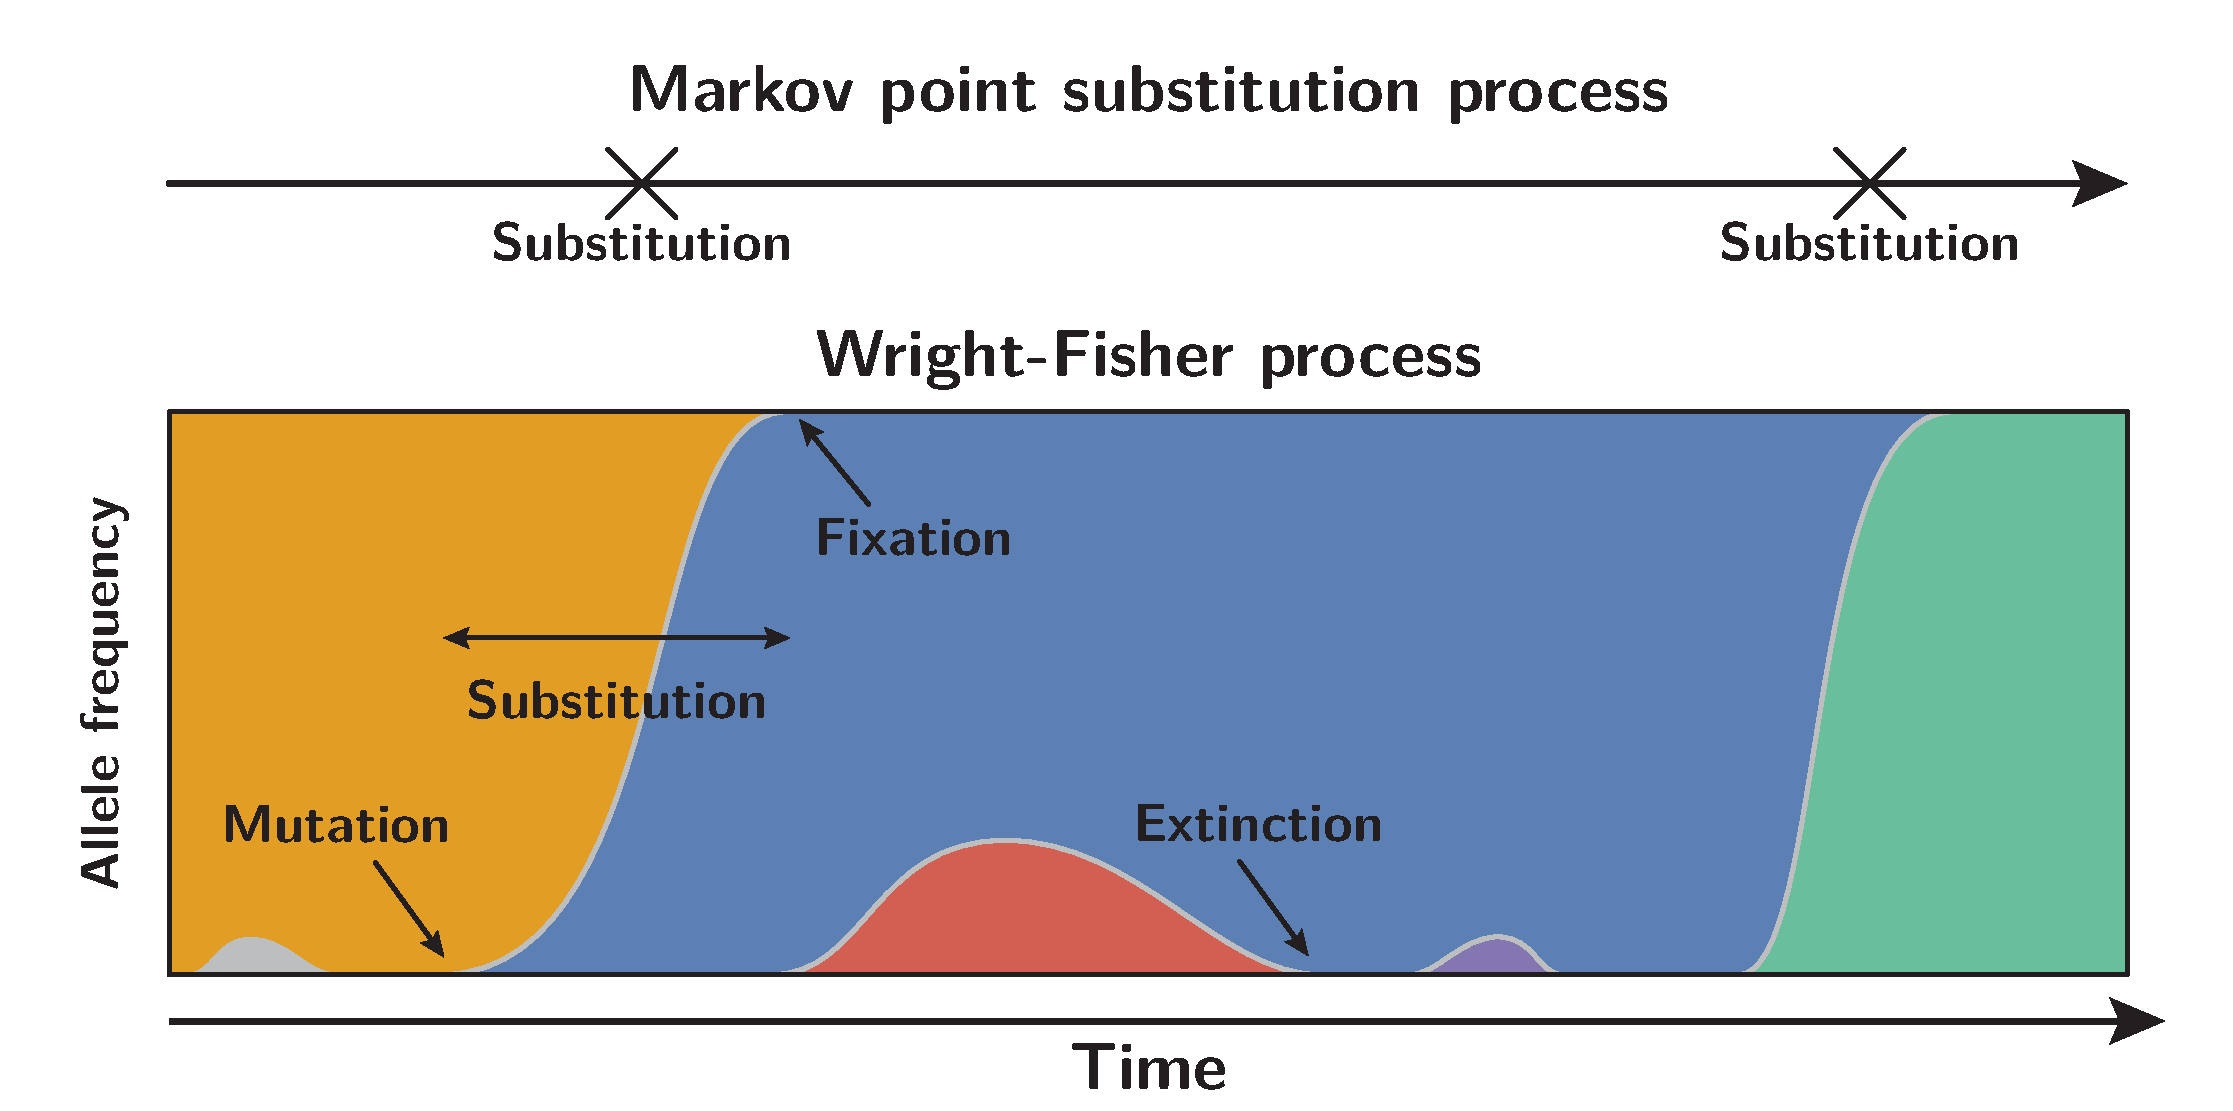
\includegraphics[width=0.75\textwidth]{figures/point-process.pdf}
    \caption[Mutation-selection substitutions models]{
    Mutation-selection \glspl{substitution} models.
    The trajectory of \glspl{allele} inside a population is collapsed into a single point \gls{substitution} process.
    This approximation is valid under low mutation rates such that a mutation originates uniquely whenever the gene is monomorphic (with a single allele).}
    \label{fig:point-process}
\end{figure}

\subsection{Mutation-limited process}
\label{subsec:mutation-limited-assumption}

Mutation-selection probabilistic models are usually Markovian with respect to time, such that the next \gls{substitution} event depends on the current representative sequence but not on earlier sequences visited in the history of a lineage.
This continuous-time Markovian process is valid if the mutation rate is sufficiently low, such that the event of a new mutation reaching fixation is completed before the next one occurs.
Since the rate of \gls{substitution} is equal to $u$ (per generation) and that each \gls{allele} ultimately reaching fixation is segregating for an average of $4 \Ne$ generations~\citep{Kimura1969}, this assumption is broadly applicable whenever the product of population size and mutation rate per generation for the sequence is lower than $1$ ($4 \Ne u \ll 1$).
More strictly, the model would require not only that new mutations reaching fixation do so before the next \gls{substitution} occurs, but before any mutation occurs, even the ones that ultimately become extinct.
Since at each generation during the process an average of $2\Ne$ mutations are produced, the point \gls{substitution} is valid under the condition that $8\Ne^2 u \ll 1$.
In practice, the assumptions that $4 \Ne u \ll 1$ is a sufficient condition for the process to be well approximated.
Throughout this development, it is important to note that $u$ is the mutation rate for the whole sequence under consideration.

For large sequences this approximation is usually not valid, and the sequence is then decomposed into each individual site, forming a collection of independently evolving continuous-time \glspl{Markov chain}.
For such a decomposition to be valid, these models have to assume free \gls{recombination} between sites.
The mutation rate $u$ in this condition then refers to the mutation rate for each independent site, rather than the total mutation rate over the collection as a whole.
For example, \citet{Halpern1998} constructed a model for the evolution of coding sequences where each \gls{codon} site is modelled as an independent \gls{Markov chain}.

\subsection{Substitution rate}
The continuous-time \gls{Markov chain} is defined by the instantaneous rate at which transitions occur between pairs of states.
Parameters of this process are summarized in table~\ref{table:params-mutsel} for readability.

\begin{table}[H]
    \centering
    \noindent\adjustbox{max width=\textwidth}{%
    \begin{tabu}{|l|c|c|c|}
        \hline
        \textbf{Parameter} & \textbf{Symbol} & \textbf{Range} \\
        \hline\hline
        Scaled fitness & $F=4 \Ne f$ & finite, positive or negative \\
        \hline Mutation rate per time & $\mu$ & $[10^{-11}, 10^{-8}]$ per site per year \\
        \hline \Gls{substitution} rate per time & $Q$ & $[10^{-11}, 10^{-8}]$ per site per year \\
        \hline Equilibrium frequency & $\pi$ & $[0, 1]$ \\
        \hline Equilibrium frequency under mutation & $\sigma$ & $[0, 1]$ \\
        \hline Mean scaled fixation probability & $\avgpfix$ & $[0, 1]$ for purifying selection \\
        \hline
    \end{tabu}}
    \caption[Parameters of mutation-selection processes]{Parameter of mutation-selection processes used in this section (\ref{subsec:mutation-limited-assumption})}
    \label{table:params-mutsel}
\end{table}

Given the current state of \gls{allele} $A$, the rate of transition to other states can be derived using the population-genetic equations introduced above.
At each generation, the expectation for the number of possible mutants is $2\Ne u$, and each of these mutants has a probability $\pfix(s, \Ne)$ to result in a \gls{substitution}.
Altogether, the instantaneous rate of \gls{substitution} from \gls{allele} $A$ to $B$, denoted $Q_{A \to B}$, is equal to the rate of mutation ($\mu_{A \to B}$) multiplied by the probability of fixation of the mutation $\pfix(s_{A \to B}, \Ne)$ and scaled by the number of possible mutants at each generation ($2\Ne$):
\begin{align}
    Q_{A \to B} & = 2 \Ne \mu_{A \to B}  \pfix(s_{A \to B}, \Ne) \label{eq:q-pfix}
\end{align}
It is important to note that the \gls{substitution} rate and the mutation rate are in the same units, such that this equation is valid whether the rate is measured either in units of chronological time or per generation (or in branch length, which will matter later on).
As a convention, in what follows, mutation rate is denoted $u$ when measured in units of generation, and denoted $\mu$ when measured in units of time.
As a consequence, $Q$ is measured in units of time in this section.

In the case of selected mutations, the probability of fixation depends on the difference in log-fitness ($\logfit_A$ and $\logfit_B$) between the two \glspl{allele}:
\begin{align}
    Q_{A \to B} & = 2 \Ne \mu_{A \to B} \pfix(s_{A \to B}, \Ne) \\
    & = 2 \Ne \mu_{A \to B}  \dfrac{2(\logfit_{B} - \logfit_{A})}{1 - \e^{4\Ne(\logfit_{A} - \logfit_{B})} } \\
    & = \mu_{A \to B} \dfrac{F_{B} - F_{A}}{1 - \e^{F_{A} - F_{B}} }\text{, where } F = 4\Ne f \label{eq:sub-transion-rates}
\end{align}

In the case of \gls{neutral} mutations, the probability of fixation is independent of the original and target sequence, and equals $1/2 \Ne$.
As a consequence, the \gls{substitution} rate denoted $Q_{A \to B}^{0}$ simplifies to:
\begin{align}
    Q_{A \to B}^{0} & = 2 \Ne \mu_{A \to B}  \pfix(0, \Ne) \\
    & = 2 \Ne \mu_{A \to B} \dfrac{1}{2\Ne} \\
    & = \mu_{A \to B} \label{eq:sub-equal-mut}
\end{align}


If the difference of log-fitness tends to $0$, the \gls{substitution} rate is equal to the mutation rate, retrieving equation~\ref{eq:sub-equal-mut}:
\begin{equation}
    \lim\limits_{|F_{B} - F_{A}| \to 0} Q_{A \to B} =  \mu_{A \to B}
\end{equation}

Taken together, the transition rates which generate the \gls{substitution} history and ultimately the interspecific diversity is parameterized solely by mutation, selection and drift.
Consequently, from a particular history of \glspl{substitution}, one can theoretically estimate the parameters of selection, mutation and drift, although it is important to keep in mind that selection and drift are confounded.


\subsection{Reversibility of the process}
The continuous-time \gls{Markov chain} has so far been defined for $2$ \glspl{allele} but can be generalized to any number of \glspl{allele}, when the number of \glspl{allele} is discrete ($\NbrSites$) and when transition from any \gls{allele} to any other \gls{allele} is possible in one or more \glspl{substitution}.
In this configuration, the transition rates between all possible pairs of \glspl{allele} is defined by equation~\ref{eq:sub-transion-rates}, and equals $0$ whenever single step transitions are not possible.
Because any state is ultimately connected to any other state, the continuous-time \gls{Markov chain} is irreducible.
Moreover, this \gls{substitution} process is positive recurrent and aperiodic since any strictly positive transition rate is matched by a strictly positive transition for the reverse \gls{substitution}.
More precisely, the \gls{substitution} rate between two \glspl{allele} is null only if the underlying mutation rate is null, in which case the transition rate for the reverse mutation is also null, hence the transition rate for the reverse \gls{substitution} is also null.

Theoretically, for an irreducible, positive recurrent and aperiodic continuous-time \gls{Markov chain}, a necessary and sufficient condition to be reversible is given by Kolmogorov's criterion.
Kolmogorov's criterion implies that the product of transition rates through any closed loop is the same whenever the traversing is done forward or in reverse.
As an example for a \gls{Markov chain} composed of $3$ \glspl{allele} ($\ci$, $\cj$ and $\ck$), as illustrated in figure~\ref{fig:reversible-circuit}, the transition rates must satisfy the equality:
\begin{equation}
    Q_{\ci \to \cj}Q_{\cj \to \ck}Q_{\ck \to \ci} = Q_{\ci \to \ck}Q_{\ck \to \cj}Q_{\cj \to \ci}
\end{equation}

\begin{figure}[htbp]
    \centering
    \begin{tikzpicture}[->,>=stealth',auto,node distance=1.2cm and 1.6cm,semithick]
        \tikzstyle{every state}=[]

        \node[] (0) {};
        \node[state] (A) [above=of 0] {$\ci$};
        \node[state] (B) [below left=of 0] {$\cj$};
        \node[state] (C) [below right=of 0] {$\ck$};

        \path[->]
        (A) edge [BLUE,bend right=45] node [left] {$Q_{\ci \to \cj}$} (B)
        (B) edge [BLUE,bend right=45] node [below] {$Q_{\cj \to \ck}$} (C)
        (C) edge [BLUE,bend right=45] node [right] {$Q_{\ck \to \ci}$} (A)
        (B) edge [RED,bend right=15] node [left] {$Q_{\cj \to \ci}$} (A)
        (C) edge [RED,bend right=15] node [below] {$Q_{\ck \to \cj}$} (B)
        (A) edge [RED,bend right=15] node [right] {$Q_{\ci \to \ck}$} (C);
    \end{tikzpicture}
    \caption[Kolmogorov's criterion]{
    The continuous-time \gls{Markov chain} is reversible if the process fulfils Kolmogorov's criterion.
    Namely, the product of the transition rates for a closed loop is equal whether traversed in one sense (blue arrows) or the other (red arrows).}
    \label{fig:reversible-circuit}%
\end{figure}

Kolmogorov's criterion is satisfied under specific conditions for the \gls{substitution} process (\ref{eq:sub-transion-rates}):
\begin{align}
    1 ={}& \dfrac{Q_{\ci \to \cj}Q_{\cj \to \ck}Q_{\ck \to \ci}}{Q_{\ci \to \ck}Q_{\ck \to \cj}Q_{\cj \to \ci}}\\
    ={}& \dfrac{\mu_{\ci \to \cj}\mu_{\cj \to \ck}\mu_{\ck \to \ci}}{\mu_{\ci \to \ck}\mu_{\ck \to \cj}\mu_{\cj \to \ci}} \times \dfrac{(F_{\cj} - F_{\ci})(F_{\ck} - F_{\cj})(F_{\ci} - F_{\ck})}{(F_{\ck} - F_{\ci})(F_{\cj} - F_{\ck})(F_{\ci} - F_{\cj})} \notag \\
    &\ \times \dfrac{( 1 - \e^{F_{\ci} - F_{\ck}} )( 1 - \e^{F_{\ck} - F_{\cj}} )( 1 - \e^{F_{\cj} - F_{\ci}} )}{( 1 - \e^{F_{\ci} - F_{\cj}} )( 1 - \e^{F_{\cj} - F_{\ck}} )( 1 - \e^{F_{\ck} - F_{\ci}} )}, \\
    ={}& \dfrac{\mu_{\ci \to \cj}\mu_{\cj \to \ck}\mu_{\ck \to \ci}}{\mu_{\ci \to \ck}\mu_{\ck \to \cj}\mu_{\cj \to \ci}} \times -\dfrac{\cancel{(F_{\ci} - F_{\cj})}\cancel{(F_{\cj} - F_{\ck})}\cancel{(F_{\ck} - F_{\ci})}}{\cancel{(F_{\ck} - F_{\ci})}\cancel{(F_{\cj} - F_{\ck})}\cancel{(F_{\ci} - F_{\cj})}} \notag \\
    &\ \times \dfrac{( \e^{F_{\ci} - F_{\ci}} - \e^{F_{\ci} - F_{\ck}} )( \e^{F_{\ck} - F_{\ck}} - \e^{F_{\ck} - F_{\cj}} )( \e^{F_{\cj} - F_{\cj}} - \e^{F_{\cj} - F_{\ci}} )}{( \e^{F_{\ci} - F_{\ci}} - \e^{F_{\ci} - F_{\cj}} )( \e^{F_{\cj} - F_{\cj}} - \e^{F_{\cj} - F_{\ck}} )( \e^{F_{\ck} - F_{\ck}} - \e^{F_{\ck} - F_{\ci}} )}, \\
    ={}& - \dfrac{\mu_{\ci \to \cj}\mu_{\cj \to \ck}\mu_{\ck \to \ci}}{\mu_{\ci \to \ck}\mu_{\ck \to \cj}\mu_{\cj \to \ci}} \notag \\
    &\ \times \dfrac{\cancel{\e^{F_{\ci}}}( \e^{-F_{\ci}} - \e^{ - F_{\ck}} )\cancel{\e^{F_{\ck}}}( \e^{-F_{\ck}} - \e^{ - F_{\cj}} )\cancel{\e^{F_{\cj}}}( \e^{-F_{\cj}} - \e^{ - F_{\ci}} )}{\cancel{\e^{F_{\ci}}}( \e^{-F_{\ci}} - \e^{ - F_{\cj}} )\cancel{\e^{F_{\cj}}}( \e^{-F_{\cj}} - \e^{ - F_{\ck}} )\cancel{\e^{F_{\ck}}}( \e^{-F_{\ck}} - \e^{ - F_{\ci}} )}, \\
    ={}& \dfrac{\mu_{\ci \to \cj}\mu_{\cj \to \ck}\mu_{\ck \to \ci}}{\mu_{\ci \to \ck}\mu_{\ck \to \cj}\mu_{\cj \to \ci}} \dfrac{\cancel{( \e^{-F_{\ck}} - \e^{ - F_{\ci}} )}\cancel{( \e^{-F_{\cj}} - \e^{ - F_{\ck}} )}\cancel{( \e^{-F_{\ci}} - \e^{ - F_{\cj}} )}}{\cancel{( \e^{-F_{\ci}} - \e^{ - F_{\cj}} )}\cancel{( \e^{-F_{\cj}} - \e^{ - F_{\ck}} )}\cancel{( \e^{-F_{\ck}} - \e^{ - F_{\ci}} )}}, \\
    ={}& \dfrac{\mu_{\ci \to \cj}\mu_{\cj \to \ck}\mu_{\ck \to \ci}}{\mu_{\ci \to \ck}\mu_{\ck \to \cj}\mu_{\cj \to \ci}}.
\end{align}
Namely, Kolmogorov's criterion for the \gls{substitution} process is satisfied only if the mutation process is also reversible, in which case Kolmogorov's criterion is also fulfilled:
\begin{equation}
    \mu_{\ci \to \cj}\mu_{\cj \to \ck}\mu_{\ck \to \ci}=\mu_{\ci \to \ck}\mu_{\ck \to \cj}\mu_{\cj \to \ci}.
\end{equation}
This example can be generalized for any closed loop, such that the reversibility of the \gls{substitution} process is conditioned on the reversibility of the underlying mutation process, which is often assumed.

\subsection{Stationary distribution}

A realization of the \gls{Markov chain} for a long period of time results in a given proportion of the time for which the process is fixed for a specific \gls{allele}, where this proportion depends of the \gls{allele} fitness, the mutational process and $\Ne$.
Because the continuous-time \gls{Markov chain} is irreducible, positive recurrent and aperiodic, it has a unique stationary distribution $\UniDimArray{\pi}$, where $\pi_{\ci}$ corresponds to the proportion of time spent in \gls{allele} $\ci$ ($1 \leq \leq \NbrSites$) after the \gls{Markov chain} has run for an infinite amount of time.

Moreover, under the condition that the \gls{Markov chain} is time-reversible, the detailed balance for the stationary distribution is satisfied for every pair $\ci$ and $\cj$:
\begin{align}
    \dfrac{\pi_{\ci}}{\pi_{\cj}} & = \dfrac{Q_{\cj \to \ci}}{Q_{\ci \to \cj}} \\
    & = \dfrac{\mu_{\cj \to \ci}}{\mu_{\ci \to \cj}}  \dfrac{F_{\ci}-F_{\cj}}{ 1 - \e^{F_{\cj}-F_{\cj}}}  \dfrac{1 - \e^{F_{\ci} - F_{\cj}} }{F_{\cj} - F_{\ci}}\\
    & = - \dfrac{\mu_{\cj \to \ci}}{\mu_{\ci \to \cj}}  \dfrac{ \e^{F_{\ci}}(\e^{-F_{\ci}} - \e^{- F_{\cj}}) }{ \e^{F_{\cj}}(\e^{-F_{\cj}} - \e^{- F_{\ci}})}  \\
    & = \dfrac{\mu_{\cj \to \ci}}{\mu_{\ci \to \cj}} \dfrac{\e^{F_{\ci}}}{\e^{F_{\cj}}} \\
\end{align}
Under the assumption that the mutational process is also reversible, the detailed balance for the stationary distribution of the mutation process ($\UniDimArray{\sigma}$) is satisfied for every pair $\ci$ and $\cj$:
\begin{align}
    \dfrac{\mu_{\cj \to \ci}}{\mu_{\ci \to \cj}} & = \dfrac{\sigma_{\ci}}{\sigma_{\cj}}
\end{align}
Altogether, the probability $\pi_{\ci}$ to find the population in \gls{allele} $\ci$ is proportional to a function (also called a Boltzmann factor) that depends only on the fitness of \gls{allele} $\ci$, the population size, and details of the mutation process~\citep{Sella2005,Mustonen2005}:
\begin{align}
    \dfrac{\pi_{\ci}}{\pi_{\cj}} & = \dfrac{\sigma_{\ci}\e^{F_{\ci}}}{\sigma_{\cj}\e^{F_{\cj}}} \text{ and } \sum\limits_{\ci=1}^{\NbrSites}\pi_{\ci} = 1, \\
    \iff \pi_{\ci} & = \dfrac{\sigma_{\ci}\e^{F_{\ci}}}{\sum\limits_{\cj=1}^{\NbrSites} \sigma_{\cj}\e^{F_{\cj}} }, \label{eq:equilibrium-mut-sel}
\end{align}
where the denominator is a normalizing constant such that the sum of probabilities is equal to $1$.
By analogy with thermodynamic systems, the evolutionary system thus reaches a Boltzmann-like distribution with $\Ne^{-1}$ playing the role of evolutionary temperature, and the log-fitness $f$ the role of energy\footnote{At high mutation rates, the quasi-species theory provides another analogy with statistical mechanics, in which the mutation rate plays the role of temperature instead of \gls{genetic drift}.}.

\subsection{Mean scaled fixation probability}
\label{subsec:mean-scaled-fixation-probability}

Occurrence probabilities given by the stationary distribution allows one to calculate all observable quantities of interest, such as the mean fitness, or the mean mutation and \gls{substitution} rates, using standard probability theory.
One quantity of interest is the ratio of the mean \gls{substitution} rate over the mean mutation rate, called $ \avgpfix $:
\begin{align}
    \avgpfix & = \dfrac{ \langle Q \rangle }{\langle \mu \rangle},
    \label{eq:relative-sub-rate} \\
    & = \dfrac{ \sum\limits_{1 \leq \ci, \cj \leq \NbrSites} \pi_{\ci} Q_{\ci \to \cj}}{\sum\limits_{1 \leq \ci, \cj \leq \NbrSites} \pi_{\ci} \mu_{\ci \to \cj}},
\end{align}
where the notation $\langle \cdot \rangle$ denotes the statistical average, and the sum is over all possible pairs of \glspl{codon} having a certain property.
In other words, $\avgpfix$ represents the flow of \glspl{substitution} at equilibrium, normalized by the mutational flow (or mutational opportunities).

This definition can in principle be applied to any subset of \gls{codon} pairs.
A particularly important case is to sum over all possible pairs of \gls{non-synonymous} \glspl{codon} (which will be considered in the next chapter).
In that case, $\avgpfix$ captures the fundamental quantity usually referred to as $\dnds$.
However, the definition is more general.

This ratio can also be interpreted as the mean scaled fixation probability of all mutations that are being proposed at mutation selection equilibrium.
Indeed, the scaled fixation probability of a given mutation is the probability of fixation of this mutation, normalized by the fixation probability of \gls{neutral} mutations:
\begin{align}
    \dfrac{\pfix (s_{\ci \to \cj}, \Ne)}{\pfix (0, \Ne)} = \Pfix (s_{\ci \to \cj}, \Ne)
\end{align}
In addition, the probability for a given type of mutation, from $\ci$ to $\cj$, to be proposed at equilibrium, is given by:
\begin{align}
    \proba (\ci \to \cj) = \dfrac{\pi_{\ci}  \mu_{\ci \to \cj}}{ \mathcal{Z}} \text{, where } \mathcal{Z} = \sum\limits_{1 \leq \ci, \cj \leq \NbrSites} \pi_{\ci} \mu_{\ci \to \cj} \label{eq:proba-a-b}
\end{align}
And thus, the statistical average at equilibrium is:
\begin{align}
    \left\langle \Pfix \right\rangle & = \sum\limits_{1 \leq \ci, \cj \leq \NbrSites}  \proba (\ci \to \cj) \Pfix (s_{\ci \to \cj}, \Ne), \\
    & = \dfrac{ \sum\limits_{1 \leq \ci, \cj \leq \NbrSites} \pi_{\ci} Q_{\ci \to \cj}}{\sum\limits_{1 \leq \ci, \cj \leq \NbrSites} \pi_{\ci} \mu_{\ci \to \cj}} \text{, from equation~\ref{eq:q-pfix} and~\ref{eq:proba-a-b}}, \\
    & = \avgpfix.
\end{align}
As a result of this definition, $\avgpfix=1$ for genes or sites under \gls{neutral} evolution.
Most importantly, departure from $1$ would be interpreted as a signature of selection on sequences.
First, $\avgpfix>1$ is interpreted as a signal of adaptive recurrent evolution, since this means that $\pfix > 1/2 \Ne$ on average.
On the other hand, $\avgpfix<1$ is a signal of underlying purifying selection such that the sequence is constrained on average.
Of note, $ \avgpfix > 1$ (or $ < 1$) does not necessarily mean that the selection coefficients are positive (or negative) on average.
Finally, a mutation-selection point \gls{substitution} process at equilibrium under a time-independent fitness landscape results in $\avgpfix \leq 1$, as demonstrated in \citet{Spielman2015}.


\section{Mutation-selection analogy in other scientific fields}

Presented in the context of phylogenetic evolution of genetic sequences, the mutation-selection process bears many similarities and analogies between other processes present in a variety of scientific fields outside of evolutionary biology, displaying the same underlying mechanism and emerging properties, though with different names and aspirations.
This section is an attempt to describe analogous processes and their emerging properties.
This effort is made in the aim of giving another view of the mutation-selection process, such as to better appreciate and conceptualize its assumptions, its limits, and the respective role of the different components.
Such attempts require to boil down the mutation-selection mechanism into its core components, while at the same time rephrasing the description using lexicography outside of population genetics such as to open new perceiving angles.

\subsection{Metropolis-Hastings sampling}
Obtaining a sequence of random samples from a probability distribution can be difficult, especially when the number of dimensions is high.
However, the Metropolis-Hastings procedure based on a \gls{Markov chain Monte Carlo} can sample from any probability distribution, provided that we know how to compute the probability density, or even less restrictively any function proportional to the density~\citep{Hastings1970}.
This stochastic procedure which is based on three steps bears many similarities with the mutation-selection process:
\begin{itemize}
    \item Generate a stochastic candidate from the current state, analogous to mutation.
    \item Calculate the acceptance ratio as the ratio of the two densities, analogous to the selection coefficient of the mutated state.
    \item Stochastic acceptance or rejection based on the acceptance ratio, a process analogous to drift.
\end{itemize}
Inherently, the Metropolis-Hastings procedure is based on creating and subsequently reducing diversity, which allows to obtain a random sequence of samples from any distribution with a straightforward recipe, and is a critical
tool in statistics and statistical physics.

\subsection{The exploration-exploitation dilemma}
Many mathematical, engineering and daily-life problems are not about sampling a state space, but rather about finding the optimal and best state given the criteria or a function to maximize.
Naturally, we would prefer deterministic (strictly reproducible) rather than stochastic optimizing strategies to search for an optimal state.
Unfortunately, whenever the state space is too large, often due to the curse of dimensionality, a greedy or heuristic search of an optimal state can perform atrociously~\citep{Bellman1966}.
In high-dimensional space, stochastic optimization tools have been deemed very valuable, such as stochastic gradient descent or so-called evolutionary algorithms~\citep{Russell2010,Vikhar2017}.
Inherently, they are based on two processes, one is stochastically creating diversity and exploring the state space, while the other is filtering the explored states and thus reducing the diversity.

In the constrained case of a finite amount of time or attempts to find the best outcome overall, the problem is best described by the multi-armed bandit problem.
The name comes from imagining a gambler at a row of slot machines (sometimes known as one-armed bandits), where each slot machine provides a random reward from a probability distribution specific to that machine. The player has to decide which machines to play, how many times to play each machine and in which order to play them, and whether to continue with the current machine or try a different machine, such as to maximize the sum of rewards earned through a sequence of trials.
The gambler faces a dilemma at each trial, either reducing his regret by exploiting the best arm, or gaining information through exploration of other arms.
The best strategy to solve this dilemma can be mathematically derived in numerous cases, and encompasses mixing strategies with a defined ratio of exploration and exploitation~\citep{Auer2002,Kocsis2006,Furnkranz2006}.
This problem is far from being only theoretical, and has been used to explain a multitude of phenomena, such as the movement of animals in novel landscapes, the most efficient resource allocation for a start-up company, the effects of age on knowledge acquisition in humans, and in the search of the most efficient treatment in clinical trials~\citep{Berger-Tal2014, March}.
Another application of the exploration-exploitation dilemma is AlphaGo, the first computational program mastering the board game Go at the professional 9-dan level in 2017, which outcompeted Ke Jie, the world first ranked player at the time~\citep{Silver2017, Silver2018}.
AlphaGo has often been publicized and hyped in various media outlets stating that this feat was possible due to machine learning, more specifically due to convolutional neural networks.
However, it is more scarcely mentioned that the AlphaGo neural network is combined with an exploration-exploitation algorithm, or more specifically a Monte Carlo tree search.
In practice, the convolutional neural network is used as a criterion to measure the advantage of a board configuration\footnote{Convolutional neural networks also use a stochastic gradient descent to reach convergence, inherently leveraging the stochastic exploration and exploitation procedure to optimize the parameters of the neural network.}, but the different moves and paths probed and trimmed are done via an exploration-exploitation procedure.

\subsection{Interaction between analogies}

At the bottom, mutation is a process creating diversity, changing and moving the current viable state to a novel and unknown position, fundamentally allowing exploration of the state space.
On the other hand, selection is the criteria on which a new state is deemed a disrupting innovation or a nonviable alteration, and allows to determine which changes to exploit and which to filter out and discard based on its fitness.
Fundamentally, mutation creates diversity and selection reduces this diversity by selecting the fittest mutants.
Finally, drift arbitrates between the creation and reduction of the two processes, it dictates how much exploration of novelty is permitted, and conversely how much exploitation of only the fittest states is granted.

Exploration and exploitation, creation and reduction, mutation and selection, are different names (see table~\ref{table:intro-mutsel-analogy}) that ultimately encompass the inherently same process: efficiently sampling and optimizing whenever the state space is too large to be traversed in a finite amount of time.

\begin{table}[H]
    \centering
    \noindent\adjustbox{max width=\textwidth}{%
    \begin{tabu}{|c|c|c|}
        \hline
        \textbf{Mutation} & \textbf{Selection} & \textbf{Drift} \\ \hline
        \hline Exploration & Exploitation & Trade-off \\
        \hline Creation & Reduction & Arbitration \\
        \hline Candidate generation & Acceptance & Hastings ratio \\
        \hline
    \end{tabu}}
    \caption[Mutation, selection and drift analogy]{
    Mutation, selection and drift lexicographic rephrasing in different fields.
    }
    \label{table:intro-mutsel-analogy}
\end{table}

I argue that evolutionary biologists, studying and leveraging the pervasive process of mutation and selection, can gain knowledge by recruiting insight and developments from other fields, much like there has been many crossovers between economics and evolution in the context of game theory.\footnote{Game theory was originally developed to model economic actors' behaviour and strategies~\citep{VonNeumann1947}. It was later adopted within the framework of evolutionary dynamics, helping to explain, for example, the emergence of altruistic behaviour in Darwinian evolution~\citep{Smith1973, Smith1982, Nowak2006}.}.

As an example of such insight from the exploration-exploitation dilemma is the understanding of the relationship between mutation rate and chromosome size.
It has been observed that organisms with a low mutation rate (per site per generation) also tend to have a long chromosome size, such that the product of genome size and mutation rate is constant~\citep{Drake1991}.
An explanation for this pervasive negative correlation between mutation rate and genome size invoke the drift barrier hypothesis, where the correlation is inherently due to underlying changes in genetic drift~\citep{Lynch2016a}.
The drift barrier hypothesis posits that selection operates to minimize the mutation rate, with the efficiency of such improvement eventually being overcome by random \gls{genetic drift}, such that populations with higher population size have smaller mutation rates.
On the other hand, a higher population size induces stronger purifying selection which reduces genome size by expelling transposable elements.
Altogether, both high mutation rate and a smaller genome are consequences of a higher population size.
An alternative explanation for the negative correlation between mutation rate and genome size is that for each new generation, the genetic diversity of offspring must balance the trade-off between exploration of new genotypes and the reliable transmission of the current one.
The genetic difference between parents and offspring is the product of mutation rate and genome size, such that individuals who are too variable undergo deleterious mutations and disappear, whereas individuals whose genotypes are not variable enough are outcompeted by those that were able to discover innovations~\citep{Knibbe2007, Beslon2010, Hindre2012, Batut2014, Biller2016}.

From a political standpoint, I also argue that scientific research endeavour is also an exploration-exploitation dilemma, which is arguably externally pressured to pursue exploitation, through funding of impactful research and a publish-or-perish systemic culture in the early career stage.

\chapter{Selection in protein coding {DNA} sequences}
{
	\hypersetup{linkcolor=GREYDARK}
	\minitoc
}
\label{sec:selection}
Evolutionary trajectory of sequences depends on the forces of mutation, selection and drift, which acts conjointly such that each one of them must be well studied and understood.
However, the previous chapter remained so far elusive on selection, and did not yet question what determines the strength of selection.
More precisely, molecular evolution requires either a given selection coefficient associated to mutation, or that the fitness of each particular sequence to be defined.
In other word, the relationship between sequence and fitness must be elucidated, which is the focus of the present chapter in the special case of protein coding \acrshort{DNA} sequence.
It will seek to clarify the relationship between protein sequence, protein thermodynamic, protein function, and organismal fitness, such as to derive the selective pressures shaping proteins coding \acrshort{DNA} sequences.
It is also important to emphasize whether they are general principles, or do this relationship between sequence and fitness depends on the specific protein, organism, and environment.
To this aims, this chapter will first present the genetic code and classical phylogenetic \glspl{codon} models, which can quantify the strength of selection acting on proteins trough an aggregate parameter (called $\omega$ or $\dnds$).
Application of these phylogenetic models to empirical \acrshort{DNA} alignment provides insight on the variation of selective strength between different orthologous genes, between sites of the same protein, or between branches of the phylogenetic tree.
Subsequently, physico-chemical constrains of proteins and thermodynamics models of protein selection are related to these empirical results.
Finally, given the results on empirical data, generalization of \gls{codon} models into the context of fitness landscapes are presented.

\section{Protein coding \acrshort{DNA} sequences}

Proteins have a variety of molecular and cellular roles, they are the enzymes that catalyses chemical bonds, they regulate cell processes and control their rates, they carry signals within the cell and across membranes, they bind and transport small molecules, they form cellular structures, and so on.
This variety of roles is accomplished by a variety of three-dimensional shapes.
A protein's three-dimensional shape is in turn determined by the linear one-dimensional sequence of amino-acids, with their size ranging from fewer than $20$ to more than $5000$ amino acids, with an average of about 350 amino-acids.
Just as \acrshort{DNA} is oriented because of the asymetry of nucleotides, proteins are oriented due to asymetry of amino-acids, one end is called \gls{N-ter} and the other end C-terminus, and each amino-acid will interact with the other amino-acids in its spatial vicinity. 

Although each of the 20 different amino acids has unique biochemical properties, they can be classified broadly into four categories determining their solubility and acidity (classification is given in table \ref{table:genetic_code}).
Charged amino-acids can be either basic (positively charged) or acidic (negatively charged).
On the other hand, non charged amino-acids can however be polar due to an uneven charge distribution, such that they can form hydrogen bonds with water.
Consequently, polar amino acids are called hydrophilic, and are often found on the outer surface of folded proteins.
Also, non charged amino-acids can have a uniform charge distribution, and do not form hydrogen bonds with water.
Reciprocally, these non polar amino-acids are called hydrophobic and tend to be found in the core of folded proteins.

\subsection{Genetic code}

Because the $20$ letter alphabet of proteins is different to the $4$ letter alphabet of nucleic acid (DNA and RNA), there is not a one-to-one correspondence between the two alphabets.
Instead, amino acids are encoded by \glspl{codon}, a consecutive sequences of 3 nucleotides, yielding $4^3=64$ possible permutations, more than sufficient to encode the 20 different amino acids.
Moreover, three stop \glspl{codon} signals termination of the protein, such that 61 of the 64 \glspl{codon} are used to encode amino acids.
Since there are 61 coding \glspl{codon} and only 20 amino acids, there is a necessary redundancy in the code.
Thus, amino-acids are encoded by synonymous \glspl{codon}, which are interchangeable in the sense of producing the same amino acid, with the notable exception of methionine and tryptophan.
Altogether, the \acrshort{DNA} genetic code translating \gls{codon} to amino-acids, which is used almost universally by all organisms is given in table \ref{table:genetic_code}.

\begin{table}[H]
	\centering
	\noindent\adjustbox{max width=\textwidth}{%
		\begin{tabular}{|c||l|c|l|c|l|c|l|c||c|}
			\hhline{|-||-|-|-|-|-|-|-|-||-|}
			& \multicolumn{2}{c|}{\textbf{T}} & \multicolumn{2}{c|}{\textbf{C}} & \multicolumn{2}{c|}{\textbf{A}} & \multicolumn{2}{c||}{\textbf{G}} & \\
			\hhline{=#========#=}
			\multirow{4}{*}{\textbf{T}} & TTT & \cellcolor{Nonpolar} & TCT & \cellcolor{Polar} & TAT & \cellcolor{Polar} & TGT & \cellcolor{Polar} & \textbf{T} \\
			\cline{2-2} \cline{4-4} \cline{6-6} \cline{8-8} \cline{10-10}
			& TTC & \cellcolor{Nonpolar} \multirow{-2}{*}{Phenylalanine (Phe/P)} & TCC & \cellcolor{Polar} & TAC & \cellcolor{Polar} \multirow{-2}{*}{Tyrosine (Tyr/Y)} & TGC & \cellcolor{Polar} \multirow{-2}{*}{Cysteine (Cys/C)} & \textbf{C} \\
			\hhline{|~||-|-|-|>{\arrayrulecolor{Polar}}->{\arrayrulecolor{black}}|-|-|-|-||-|}
			& TTA & \cellcolor{Nonpolar} & TCA & \cellcolor{Polar} & TAA & \cellcolor{Stop} Stop (Ochre) & TGA & \cellcolor{Stop} Stop (Opal) & \textbf{A} \\
			\hhline{|~||-|>{\arrayrulecolor{Nonpolar}}->{\arrayrulecolor{black}}|-|>{\arrayrulecolor{Polar}}->{\arrayrulecolor{black}}|-|-|-|-||-|}
			& TTG & \cellcolor{Nonpolar} & TCG & \cellcolor{Polar} \multirow{-4}{*}{Serine (Ser/S)} & TAG & \cellcolor{Stop} Stop (Amber) & TGG & \cellcolor{Nonpolar} Tryptophan (Trp/W) & \textbf{G} \\
			\hhline{|-||-|>{\arrayrulecolor{Nonpolar}}->{\arrayrulecolor{black}}|-|-|-|-|-|-||-|}
			\multirow{4}{*}{\textbf{C}} & CTT & \cellcolor{Nonpolar} & CCT & \cellcolor{Nonpolar} & CAT & \cellcolor{Basic} & CGT & \cellcolor{Basic} & \textbf{T} \\
			\cline{2-2} \cline{4-4} \cline{6-6} \cline{8-8} \cline{10-10}
			& CTC & \cellcolor{Nonpolar} & CCC & \cellcolor{Nonpolar} & CAC & \cellcolor{Basic} \multirow{-2}{*}{Histidine (His/H)} & CGC & \cellcolor{Basic} & \textbf{C} \\
			\hhline{|~||-|>{\arrayrulecolor{Nonpolar}}->{\arrayrulecolor{black}}|-|>{\arrayrulecolor{Nonpolar}}->{\arrayrulecolor{black}}|-|-|-|>{\arrayrulecolor{Basic}}->{\arrayrulecolor{black}}||-|}
			& CTA & \cellcolor{Nonpolar} & CCA & \cellcolor{Nonpolar} & CAA & \cellcolor{Polar} & CGA & \cellcolor{Basic} & \textbf{A} \\
			\cline{2-2} \cline{4-4} \cline{6-6} \cline{8-8} \cline{10-10}
			& CTG & \cellcolor{Nonpolar} \multirow{-6}{*}{Leucine (Leu/L)} & CCG & \cellcolor{Nonpolar} \multirow{-4}{*}{Proline (Pro/P)} & CAG & \cellcolor{Polar} \multirow{-2}{*}{Glutamine (Gln/Q)} & CGG & \cellcolor{Basic} \multirow{-4}{*}{Arginine (Arg/R)} & \textbf{G} \\
			\hhline{|-||-|-|-|-|-|-|-|-||-|}
			\multirow{4}{*}{\textbf{A}} & ATT & \cellcolor{Nonpolar} & ACT & \cellcolor{Polar} & AAT & \cellcolor{Polar} & AGT & \cellcolor{Polar} & \textbf{T} \\
			\cline{2-2} \cline{4-4}\cline{6-6} \cline{8-8} \cline{10-10}
			& ATC & \cellcolor{Nonpolar} & ACC & \cellcolor{Polar} & AAC & \cellcolor{Polar} \multirow{-2}{*}{Asparagine (Asn/N)} & AGC & \cellcolor{Polar} \multirow{-2}{*}{Serine (Ser/S)} & \textbf{C} \\
			\hhline{|~||-|>{\arrayrulecolor{Nonpolar}}->{\arrayrulecolor{black}}|-|>{\arrayrulecolor{Polar}}->{\arrayrulecolor{black}}|-|-|-|-||-|}
			& ATA & \cellcolor{Nonpolar} \multirow{-3}{*}{Isoleucine (Ile/I)} & ACA & \cellcolor{Polar} & AAA & \cellcolor{Basic} & AGA & \cellcolor{Basic} & \textbf{A} \\
			\hhline{|~||-|-|-|>{\arrayrulecolor{Polar}}->{\arrayrulecolor{black}}|-|>{\arrayrulecolor{Basic}}->{\arrayrulecolor{black}}|-|>{\arrayrulecolor{Basic}}->{\arrayrulecolor{black}}||-|}
			& ATG & \cellcolor{Nonpolar} Methionine (Met/M) & ACG & \cellcolor{Polar} \multirow{-4}{*}{Threonine (Thr/T)} & AAG & \cellcolor{Basic} \multirow{-2}{*}{Lysine (Lys/K)} & AGG & \cellcolor{Basic} \multirow{-2}{*}{Arginine (Arg/R)} & \textbf{G} \\
			\hhline{|-||-|-|-|-|-|-|-|-||-|}
			\multirow{4}{*}{\textbf{G}} & GTT & \cellcolor{Nonpolar} & GCT & \cellcolor{Nonpolar} & GAT & \cellcolor{Acidic} & GGT & \cellcolor{Nonpolar} & \textbf{T} \\
			\cline{2-2} \cline{4-4} \cline{6-6} \cline{8-8} \cline{10-10}
			& GTC & \cellcolor{Nonpolar} & GCC & \cellcolor{Nonpolar} & GAC & \cellcolor{Acidic} \multirow{-2}{*}{Aspartic acid (Asp/D)} & GGC & \cellcolor{Nonpolar} & \textbf{C} \\
			\hhline{|~||-|>{\arrayrulecolor{Nonpolar}}->{\arrayrulecolor{black}}|-|>{\arrayrulecolor{Nonpolar}}->{\arrayrulecolor{black}}|-|-|-|>{\arrayrulecolor{Nonpolar}}->{\arrayrulecolor{black}}||-|}
			& GTA & \cellcolor{Nonpolar} & GCA & \cellcolor{Nonpolar} & GAA & \cellcolor{Acidic} & GGA & \cellcolor{Nonpolar} & \textbf{A} \\
			\cline{2-2} \cline{4-4} \cline{6-6} \cline{8-8} \cline{10-10}
			& GTG & \cellcolor{Nonpolar} \multirow{-4}{*}{Valine (Val/V)} & GCG & \cellcolor{Nonpolar} \multirow{-4}{*}{Alanine (Ala/A)} & GAG & \cellcolor{Acidic} \multirow{-2}{*}{Glutamic acid (Glu/E)} & GGG & \cellcolor{Nonpolar} \multirow{-4}{*}{Glycine (Gly/G)} & \textbf{G} \\
			\hhline{|-||-|-|-|-|-|-|-|-||-|}
	\end{tabular}}
	\caption[The Genetic Code]{
		The genetic code \acrshort{DNA} table translating \glspl{codon} into amino-acids.
		Amino-acids are represent into $4$ categories based on the electrochemical properties.
		Non-polar in yellow (\textcolor{Nonpolar}{\ding{110}}), polar in green (\textcolor{Polar}{\ding{110}}), basic in blue (\textcolor{Basic}{\ding{110}}) and finally acidic in red (\textcolor{Acidic}{\ding{110}}).
		Stop \glspl{codon} are represented in black (\textcolor{Stop}{\ding{110}}).
		The synonymous \glspl{codon} encoding for the same amino-acid are usually different by their third \gls{codon} position, the wooble base.
	}
	\label{table:genetic_code}
\end{table}

Biochemical translation from \gls{codon} to amino-acid mechanistically emanates from transfer \acrshort{RNA} (\acrshort{tRNA}).
More precisely, \glspl{codon} binds to \acrshort{tRNA} via an anticodon, three consecutive bases that are complementary and antiparallel to the associated \gls{codon}.
On the other end, \acrshort{tRNA} structure complexes uniquely with one the $20$ amino acid, where the catalytic reaction is performed by aminoacyl-tRNA synthetase \citep{Rich1976}.
As a result, \acrshort{tRNA} genes along with aminoacyl-tRNA synthetase genes constitute the machinery necessary for translating \glspl{codon} into amino-acids .
However, there is not a one-to-one correspondence between the $61$ \glspl{codon} and \acrshort{tRNA} genes.
First, the set of unique sequence of anticodon found in tRNAs genes is actually lower than $61$, and depends on the species but varies from $41$ to $55$ \citep{Goodenbour2006}.
This subset of anticodon sequences necessary to binds all $61$ \glspl{codon} is due to non canonical base pairing\footnote{Canonical base pairing are A-U and G-C, where thymin (T) is replaced by uracil (U) in RNA}.
More precisely, the first two positions in the \gls{codon} bond strongly to the anticodon of the \acrshort{tRNA} (second and third positions), while the third base of the \gls{codon} can be subject to non standard pairing with the first base of the anticodon.
If the anticodon contains a guanine at first position, \glspl{codon} with either U or C at the third position can bounds to this anticodon, and this phenomenon explains why there is not any non-synonymous {transition} from only U to C at third position, and why synonymous \glspl{codon} usually end with T or C.
Also, if the anticodon contains an Inosine at first position, \glspl{codon} with either C, U or A at the third position can bounds to this anticodon, such that for example Leucine encoded by three \gls{codon} (AUU, AUC, AUA) can be bounded by the unique anticodon IAU.
Altogether, non-standard pairing explains why the number of unique anticodons is lower than the number of possible \glspl{codon}, and also explains some part of the structure of the genetic code.

Secondly, \acrshort{tRNA} genes with the same amino-acid binding site and anticodon, which are called isoacceptor \acrshort{tRNA}, may vary in other parts of the \acrshort{tRNA} sequence.
Effectively, many genes can codes for the same isoacceptor \acrshort{tRNA}, where each gene can display varying efficiency and errors in translation, adding a layer of regulation to the process of protein synthesis \citep{Lowe1997,Chan2008,Juhling2008,Lin2019}.
As a result, in some genes some \glspl{codon} are more frequently represented than other possible synonymous \glspl{codon}, an effect named \gls{codon} usage bias.
For genes that are expressed at high levels, the \gls{codon} use is biased in favor of the \glspl{codon} that have an high \acrshort{tRNA} concentration in the cell, ultimately increasing the expression rate and decreasing the rate of mistranslation by reducing the time of occupancy of an open site.
Thus, at a fine-grained molecular scope, a synonymous change can influence mRNA stability, splicing process and protein-folding during translation \citep{Plotkin2011, Rak2018}.
However in the scope of this manuscript, such selection between synonymous \glspl{codon} will not be considered, and selection for proteins will be framed at the amino-acid level in first approximation, and mutation at the nucleotide level.
\begin{table}[H]
	\centering
	\noindent\adjustbox{max width=\textwidth}{%
	\begin{tabu}{|c||c|c|c|c|c|c|c|c|c|c|c|c|c|c|c|c|c|c|c|c|}
		\hline & \textbf{K} & \textbf{N} & \textbf{T} & \textbf{R} & \textbf{S} & \textbf{I} & \textbf{M} & \textbf{Q} & \textbf{H} & \textbf{P} & \textbf{L} & \textbf{E} & \textbf{D} & \textbf{A} & \textbf{G} & \textbf{V} & \textbf{Y} & \textbf{C} & \textbf{W} & \textbf{F}\\
		\hline
		\hline \textbf{K} & - & 4 & 2 & 2 & 0 & 1 & 1 & 2 & 0 & 0 & 0 & 2 & 0 & 0 & 0 & 0 & 0 & 0 & 0 & 0\\
		\hline \textbf{N} & - & - & 2 & 0 & 2 & 2 & 0 & 0 & 2 & 0 & 0 & 0 & 2 & 0 & 0 & 0 & 2 & 0 & 0 & 0\\
		\hline \textbf{T} & - & - & - & 2 & 6 & 3 & 1 & 0 & 0 & 4 & 0 & 0 & 0 & 4 & 0 & 0 & 0 & 0 & 0 & 0\\
		\hline \textbf{R} & - & - & - & - & 6 & 1 & 1 & 2 & 2 & 4 & 4 & 0 & 0 & 0 & 6 & 0 & 0 & 2 & 2 & 0\\
		\hline \textbf{S} & - & - & - & - & - & 2 & 0 & 0 & 0 & 4 & 2 & 0 & 0 & 4 & 2 & 0 & 2 & 4 & 1 & 2\\
		\hline \textbf{I} & - & - & - & - & - & - & 3 & 0 & 0 & 0 & 4 & 0 & 0 & 0 & 0 & 3 & 0 & 0 & 0 & 2\\
		\hline \textbf{M} & - & - & - & - & - & - & - & 0 & 0 & 0 & 2 & 0 & 0 & 0 & 0 & 1 & 0 & 0 & 0 & 0\\
		\hline \textbf{Q} & - & - & - & - & - & - & - & - & 4 & 2 & 2 & 2 & 0 & 0 & 0 & 0 & 0 & 0 & 0 & 0\\
		\hline \textbf{H} & - & - & - & - & - & - & - & - & - & 2 & 2 & 0 & 2 & 0 & 0 & 0 & 2 & 0 & 0 & 0\\
		\hline \textbf{P} & - & - & - & - & - & - & - & - & - & - & 4 & 0 & 0 & 4 & 0 & 0 & 0 & 0 & 0 & 0\\
		\hline \textbf{L} & - & - & - & - & - & - & - & - & - & - & - & 0 & 0 & 0 & 0 & 6 & 0 & 0 & 1 & 6\\
		\hline \textbf{E} & - & - & - & - & - & - & - & - & - & - & - & - & 4 & 2 & 2 & 2 & 0 & 0 & 0 & 0\\
		\hline \textbf{D} & - & - & - & - & - & - & - & - & - & - & - & - & - & 2 & 2 & 2 & 2 & 0 & 0 & 0\\
		\hline \textbf{A} & - & - & - & - & - & - & - & - & - & - & - & - & - & - & 4 & 4 & 0 & 0 & 0 & 0\\
		\hline \textbf{G} & - & - & - & - & - & - & - & - & - & - & - & - & - & - & - & 4 & 0 & 2 & 1 & 0\\
		\hline \textbf{V} & - & - & - & - & - & - & - & - & - & - & - & - & - & - & - & - & 0 & 0 & 0 & 2\\
		\hline \textbf{Y} & - & - & - & - & - & - & - & - & - & - & - & - & - & - & - & - & - & 2 & 0 & 2\\
		\hline \textbf{C} & - & - & - & - & - & - & - & - & - & - & - & - & - & - & - & - & - & - & 2 & 2\\
		\hline \textbf{W} & - & - & - & - & - & - & - & - & - & - & - & - & - & - & - & - & - & - & - & 0\\
		\hline \textbf{F} & - & - & - & - & - & - & - & - & - & - & - & - & - & - & - & - & - & - & - & -\\
		\hline
	\end{tabu}}
\caption[Amino-acids adjacency matrix]{
Number of possible one nucleotide non-synonymous {transitions} between amino-acids, integrating over the underlying \glspl{codon}.
For all the possible $190$ pairs of amino-acids, only $75$ pairs contains at least one non-synonymous {transition}.
}
\label{table:adjacency}
\end{table}
Because mutations are at the nucleotide level and affect only one base, any \gls{codon} can have at most $9$ possible {transitions} to another \glspl{codon} as illustrated in the left panel of figure \ref{fig:graph-codons-aa}.
Moreover, it is possible that some pairs of amino-acids are not accessible through a single non-synonymous {transition} between the underlying \glspl{codon} as illustrated in the right panel of figure \ref{fig:graph-codons-aa}.
In fact, most pairs of amino-acids requires at least two non-synonymous {transitions} ($114$ pairs), in comparison to pairs of amino-acids that are accesible trough a single non-synonymous {transition} ($75$ pairs).

\begin{figure}[htbp!]
	\centering
		\begin{minipage}{0.49\linewidth}
			\includegraphics[width=\linewidth, page=1]{figures/gt-codon-tab20b.pdf}
		\end{minipage}%
		\hfill
		\begin{minipage}{0.49\linewidth}
			\includegraphics[width=\linewidth, page=1]{figures/gt-aa-tab20b.pdf}
		\end{minipage}

	\caption[Graphs of \gls{codon} and amino-acid transitions]{
		\label{fig:graph-codons-aa}
		Graphs of possible one nucleotide {transition} between \gls{codon} (left panel) and between amino-acid (right panel).
		Nodes corresponds to \glspl{codon} (left panel) and amino-acid (right panel), where their color pictures the encoded amino-acid.
		Additionanly, for amino-acids the size of nodes represent the number of underlying \glspl{codon}.
		An edge between two \glspl{codon} depicts a one nucleotide {transition}, such that a \gls{codon} can have at most $9$ possible {transitions}.
		Similarly, an edge between two amino-acids correspond to a one nucleotide non-synonymous {transition} between the underlying \glspl{codon}, and the weight of the edges represent the number such possible {transitions}.
		Non-synonymous {transition} are represented in colored gradient, while synonymous {transitions} are depicted in black.
		The graph of the $61$ \glspl{codon} contains $263$ {transitions}, $67$ of them are syonymous while $196$ are non-synonymous.
		The radius of the graph is three, such that the most distant amino-acids are at most three {transition} away.
		Codons encoding for the same amino-acid are all fully connected by synonymous changes, expect for Serine where a {transition} for (TCT, TCG, TCC,	TCA) to (AGT, AGC) requires passing trought another amino-acid, hence a least two non-synonymous {transitions}.
		From the perspective of amino-acids, the graph of the $20$ amino-acids contains $75$ non-synonymous {transitions}.
		The graph is not fully connected and do not form a clique. Moreover, the graph radius equal to three because a {transition} from Methione to Tyrosine requires at least three non-synonymous {transitions}.
		Altogether, for all the possible $190$ pairs of amino-acids, $114$ pairs requires at least two non-synonymous {transitions}, and one pair (M-Y) requires at least three non-synonymous {transitions}.
	}
\end{figure}

\subsection{Codon \gls{substitution} models}
Under the approximation that selection occurs for protein, designing \gls{substitution} models at the amino-acid level has the major shortcoming of not taking into account that the underlying mutation process occurs at the nucleotide level.
Conversely, studying evolution of protein coding \acrshort{DNA} sequences only at the nucleotide level, while disregarding the genetic code neglects the consequences that nucleotide variation can have onto protein sequences.
These shortcomings are both addressed by \gls{codon} models, where the complexity of the genetic code is seen as an asset rather than an encumbrance.
Indeed the redundancy in the genetic code can be leveraged to disentangle mutation and selection in protein coding \acrshort{DNA} sequences, under the approximation that selection occurs at the protein level in first approximation, while the mutation process occurs at the \acrshort{DNA} level.
The genetic code allows to split mutations into synonymous and non-synonymous mutations, where synonymous mutations are deemed \gls{neutral}, and non-synonymous mutations are considered under selection \citep{Muse1994,Goldman1994}.

Following the formalism of \gls{codon} models pioneered by \citet{Muse1994}, the $4 \times 4$ mutation matrix $\Mutmatrix$ at the nucleotide level is defined as:
\begin{equation}
\label{eq:mutrates}
\Mutmatrix = \begin{pmatrix}
- & {\mutmatrix_{AC}} & 		{\mutmatrix_{AG}} & 		{\mutmatrix_{AT}} \\
{\mutmatrix_{AC}} & - & {\mutmatrix_{CG}} &		{\mutmatrix_{CT}} \\
{\mutmatrix_{AG}} & 		{\mutmatrix_{CG}} & - & {\mutmatrix_{GT}} \\
{\mutmatrix_{AT}} & 		{\mutmatrix_{CT}} & 		{\mutmatrix_{GT}} & -
\end{pmatrix},
\end{equation}
Grouping nucleotides into \glspl{codon}, mutation rate from \gls{codon} $\ci$ to $\cj$ thus depends on the underlying nucleotide change between the \gls{codon}, if $\ci$ to $\cj$ are only a mutation away, $\nucitoj$ denotes the nucleotide change between the \glspl{codon} and the mutation rate from \gls{codon} $\ci$ to $\cj$ is:
\begin{equation}
\mu_{\itoj} = 
\begin{dcases}
 \mutmatrix_{\nucitoj} \text{ if $\ci$ and $\cj$ are one mutation away,} \\
 0 \text{ else.}
\end{dcases}
\end{equation}

At the \gls{codon} level, synonymous mutations are deemed \gls{neutral} and the rate of \glspl{synonymous} ${\submatrix_{\itoj}}$ is equal to the mutation rate: 
\begin{align}
\submatrix_{\itoj} & = \mu_{\itoj} \\
				  & = \mutmatrix_{\nucitoj}
\end{align}

Conversely, non-synonymous mutations are considered under selection, where their probability of fixation is stretched by a factor $\omega$, and their \gls{substitution} rate is:
\begin{align}
\submatrix_{\itoj} & = \omega \mu_{\itoj} \\
					& = \omega \mutmatrix_{\nucitoj}.
\end{align}
All non-synonymous mutations are considered equivalent, and $\omega$ encompass the average strength of selection exercised on them.
Most importantly, $\omega>1$ is absorbing the signals of an excess in the rate of \glspl{non-synonymous}, indicating that the protein is under adaptive evolution.
Conversely, a default of \glspl{non-synonymous}, leading to $\omega<1$, means the protein is under purifying selection.


Because of this definition, $\omega$ identifies with the rate of \glspl{non-synonymous} over the rate of \glspl{synonymous}, termed $\dnds$.

Throughout this manuscript, the term $\dnds$ will be used to identify the estimation of $\omega$ from protein coding \acrshort{DNA} sequence alignment under the original model of \citet{Muse1994}.
To note, $\omega$ can also be parameterized as function of the average scaled selection coefficient:
\begin{align}
\omega & = \dfrac{S}{1 - \e^{-S}} \text{, where }\\
& \Rightarrow	\begin{dcases}
	S > 0 \iff \omega > 1 \\
	S = 0 \iff \omega = 1 \\
	S < 0 \iff \omega < 1
	\end{dcases}
\end{align}

Altogether, the $61$-by-$61$ \gls{codon} \gls{substitution} matrix of \citet{Muse1994} is defined entirely by the mutation matrix ($\Mutmatrix$), $\omega$ and the genetic code:
\begin{equation}
\begin{dcases}
\submatrix_{\itoj} & = 0 \text{ if $\ci$ and $\cj$ are not one mutation away} \\
\submatrix_{\itoj} & = \mutmatrix_{\nucitoj} \text{ if $\ci$ and $\cj$ are syonymous} \\
\submatrix_{\itoj} & = \omega \mutmatrix_{\nucitoj} \text{ if $\ci$ and $\cj$ are non-syonymous} \\
\submatrix_{\ci, \ci} & = - \sum_{\cj \neq \ci} \submatrix_{\itoj}
\end{dcases}
\label{eq:codon-models}
\end{equation}

It is important to note that under this model, the equilibrium frequencies of all \glspl{codon} are equal, and depends only on the equilibrium frequencies of nucleotides ($\sigma_{A}, \sigma_{C}, \sigma_{G}, \sigma_{T}$):
\begin{align}
\pi_{\ci} & = \dfrac{\sigma_{\ci[1]}\sigma_{\ci[2]}\sigma_{\ci[3]}}{\sum_{\cj}\sigma_{\cj[1]}\sigma_{\cj[2]}\sigma_{\cj[3]} } \\
 & = \dfrac{\sigma_{\ci[1]}\sigma_{\ci[2]}\sigma_{\ci[3]}}{(1 - \sigma_{T}\sigma_{A}\sigma_{A} - \sigma_{T}\sigma_{A}\sigma_{G} - \sigma_{T}\sigma_{G}\sigma_{A} )},
\end{align}
where $\ci[1]$ denotes the nucleotide at position $1$ of \gls{codon} $i$.

Moreover, the relative \gls{substitution} rate at equilibrium $\langle \nu \rangle$ defined by equation \ref{eq:relative-sub-rate}, if restricted to the subset of \glspl{non-synonymous}, identifies to $\omega$:
\begin{align}
\langle \nu \rangle & = \dfrac{ \sum_{\ci} \pi_{\ci} \sum_{\cj \in \NonSyn_{\ci}} Q_{\itoj}}{\sum_{\ci} \pi_{\ci} \sum_{\cj \in \NonSyn_{\ci}} \mu_{\itoj}} \\
					& = \dfrac{ \sum_{\ci} \pi_{\ci} \sum_{\cj \in \NonSyn_{\ci}} \omega \mu_{\itoj}}{\sum_{\ci} \pi_{\ci} \sum_{\cj \in \NonSyn_{\ci}} \mu_{\itoj}} \\
					& = \omega \dfrac{ \sum_{\ci} \pi_{\ci} \sum_{\cj \in \NonSyn_{\ci}} \mu_{\itoj}}{\sum_{\ci} \pi_{\ci} \sum_{\cj \in \NonSyn_{\ci}} \mu_{\itoj}} \\
					& = \omega, 
\end{align}
where $\NonSyn_{\ci}$ is the set of non-synonymous \glspl{codon} neighbors to \gls{codon} $\ci$.
This identity seems so far trivial and unnecessary, but will bear importance later when comparing this phenomenological model to mechanistic models of \gls{codon} \glspl{substitution}.


\section{Empirical relative rate of non-synonymous substitutions}
Models of \gls{codon} \glspl{substitution} can be to applied to protein coding \acrshort{DNA} sequences alignment to estimates the ratio of non-synonymous over \gls{synonymous} rates ($\dnds=\hat{\omega}$).
More precisely, these models can provides estimates of $\dnds$ for the whole gene, for a specific site or for a specific branch of the tree, and whether the sequence evolves under positive or negative selection.
However, in practice, protein are typically under a mix of adaptation and purifying selection, thus typically leading to an $\dnds<1$ even in the presence of positive selection.
Most importantly to the scope of this manuscript, they \gls{codon} models proved to be very valuable to quantify and asses the selective constrains imposed on protein coding sequences.

Importantly, different implementations of phylogenetic \gls{codon} models have been proposed, which parameterize the mutation matrix and the \gls{codon} frequencies in different way \citep{Muse1994, Goldman1994}, ultimately leading to variable fits of the data and different estimation of $\dnds$ on the same dataset. 
However, and fortunately, estimation of $\dnds$ has been proved to be largely insensitive to the underlying \gls{codon} models \citep{Spielman2018}, such that empirical estimation of $\dnds$ using different methods leads to comparable results.

\subsection{Variation across genes}

The increased availability of genomic data together with advancement of computing resources and algorithm prompted an extensive search for the major determining factor of a gene $\dnds$.
Surprisingly, the functional importance of a protein, widely thought to approximate the level of functional constraint, has only a minor role, whereas protein expression level (mRNA concentraion) is found to be a major determinant \citep{Zhang2015}.
Most importantly, this relationship is negative such that genes with high expression level are under stronger purifying selection, or lower $\dnds$ at the level of the gene \citep{Duret2000, Drummond2005a, Zhang2015}.
In unicellular organisms, the mRNA concentration of a gene varies across cell cycle stages and environments, but most studies used data collected from the mid-log phase of growth under rich media, which presumably reflect average concentrations across cell cycle stages.
In multicellular organisms, mRNA concentration data used are typically from the whole organism or are averaged from several examined tissues.
Because of the strong correlation between mRNA and protein concentrations, the negative correlation between protein concentration and evolutionary rate is also strong.

However, even for those proteins of comparable expression levels, their $\dnds$ still span several orders of magnitude \citep{Drummond2008}.
Abundance likewise cannot account for the quasi log-normal distribution of $\dnds$ among genes in a genome, a fact observed from bacteria, yeast, worm, fly, mouse, and humans.
These observations suggest that protein abundance, although a major determinant of $\dnds$, is not its only causal variable.

\subsection{Variation across sites}

Appart from variation across genes, the strength of selection is not typically homogeneous along the protein sequence, and it has been rapidly recognized that the parameter $\dnds$ should not be estimated globally over the entire sequence.
In so-called site-specific phylogenetic \gls{codon} models, $\dnds$ is allowed to vary across sites, either via a finite mixture \citep{Yang2001}, an infinite mixture \citep{Huelsenbeck2006}, or as random effects from a parametric distribution \citep{Lartillot2013}.
Site-specific models had been developed to detect specific site of the sequence under positive recurrent selection \citep{kosiol_patterns_2008}, with a $\dnds>1$, but also proved to be very valuable models to correlate selective pressure and bio-chemical properties os specific sites.

Similarly to search for the determining factors of $\dnds$ at the gene level, extensive search had been conducted at the site level, within a protein.
The major determinant of site-specific $\dnds$ proved to be relative solvent accessibility, where site with higher solvent accessibility display a lower $\dnds$ \citep{Ramsey2011}.
It was later shown that the number of native inter-residue contacts formed by a protein site, which is negatively correlated with the solvent accessibility, is a stronger predictor of site-specific $\dnds$ \citep{Yeh2013}.
Altogether, $\dnds$ changes dramatically between exposed and buried sites in such a way that buried sites tend to evolve more slowly than exposed sites \citep{Echave2016}.
Moreover, this relationship obtained by means of phylogenetic \gls{codon} models can be matched with experiment correlating protein site properties with allelic diversity within population.
In this context, relative solvent accessibility was also found to be a major determinant of adaptive evolution, with most adaptive mutations occurring at the surface of proteins \citep{Moutinho2019}.

The observations that surface residues of globular proteins undergo \gls{substitution} more rapidly than those in the core is generally attributed to the fact that natural selection imposes stronger constraints on buried sites.
It is well known that amino acid residues located inside a protein structure (that is, core residues) have more central roles than surface residues in protein folding stability.

Finally, it is important to keep in mind that selection differs in a way that depends on the specific source and target amino-acid involved in the {transition}.
As a consequence, a single parameter of selection (here $\dnds$) can not disentangle the specific importance of amino-acid chemical properties (polarity, volume, charge, and so on) since all non-synonymous {transitions} are considered equivalent in classical phylogenetic \gls{codon} models \citep{Dutheil2008}.

\subsection{Variation across branches}

Beside variation across genes and site, the strength of selection is not typically homogeneous along the phylogenetic tree, and it has also been recognized that the parameter $\dnds$ should be varying along the tree \citep{Yang1998}.
The motivation was to allow for $\dnds$ to be estimated only on a subset of the phylogeny, based on biological assumption.
For example, such models can detect an adaptive process ongoing during the divergence of one lineage, which can allow for the detection of the proteins responsible for speciation \citep{Yang2001, Zhang2004}.
Moreover, without \gls{prior} knowledge on biological divergence, branches can get clustered together based on their \gls{substitution} rates \citep{Dutheil2012a}.
However, \gls{substitution} rate is a continuous traits, and should evolve smoothly along the phylogeny, such that abrupt shifts are penalized \citep{Huelsenbeck2003,Seo2004}.
I this modeling approach, \gls{substitution} rate of given branch is log-normally distributed around the value of its parent branch, where the standard deviation is proportional to the branch size (in unit of time) \citep{Lartillot2011, Brevet2019}.
In other words, \gls{substitution} rate is seen as a log-Brownian motion along the phylogeny, where the process splits at every node of the tree. 

Similarly to search for the determining factors of $\dnds$ at the gene and site level, environmental variables or life-history traits that can vary between species have been investigated as factor determining $\dnds$ along the phylogeny \citep{Felsenstein1985,Romiguier2014}.
Integrative inference methods combining molecular sequences and lineage specific quantitative traits have also found that $\dnds$ correlates positively with traits such as longevity and body mass \citep{Lartillot2011, Figuet2017}.
Since lineage with a large body size and extended longevity typically correspond to low $\Ne$ \citep{Romiguier2014}, these empirical correlations suggest a negative correlation between $\dnds$ and $\Ne$, thus confirming the theoretical prediction of the \gls{nearly-neutral} theory of evolution.
However, the universality and robustness of the correlation between $\dnds$ and life-history traits is still debated \citep{Nabholz2013, Lanfear2014, Figuet2016}.

Naturally, both these space (site-specific) and time (branch-specific) refinements mentioned above where combined in so called branch-site models \citep{Yang2002, Zhang2004, Pond2011}.
The fine-grained tunning of site-branch models increased statistical power by seeking short and strong episodes of adaptive selection on a background of purifying selection.
However, in the case of Red-Queen processes ongoing on the protein, the episodes detected by branch-site models would merely be a small fraction of the underlying adaptation.
Indeed the overall tree is under adaptive process and one cannot contrast a branch to the rest of the tree.

%The selection coefficient are drawn from a distribution, known as distribution of fitness effects \citep{Welch2008}
%In Wilson, the fitness effect of a mutation is drawn from a fitness distribution that is solely function of $\Ne$, meaning ${P_{\mathrm{fix}}}$ is independent from the current sequence state.
%On the other hand, in the mutation-selection model proposed, the distribution of fitness effects is a function of the current state.
%
%Because its a distribution of fitness effects and not a fitness landscape, features of evolutionary trajectory such as transient positive selection is not represented.
%They are a generic representation of fitness, easily parameterized and inherently taking into account phenomenon such as epistasis.


\section{Protein biophysics}

The ability of a protein to performs its function depends on the stability of its 3-dimensional folding structure, but also on its ability to bind ligands and interact or no with other protein, both in terms of kinetic and stability.
Altogether, thermodynamics and kinetic of protein are expected to be related to its function, hence to selective constrains \citep{Bastolla2017}.
This section review the main relationship between protein biophysics and selection.
\textcolor{GREEN}{[I should be working on a better {transition} between classical \gls{codon} models and protein biophysics]}.
\subsection{Stability constrains}

First, a large body of evidence indicates that the stability of globular proteins is a target of natural selection \citep{Sikosek2014}.
The stability of a protein is determined by the Gibbs free energy of its folded states, in comparison to the free energy of the unfolded states.
Similarly to the mutation-selection Markov process defined in the previous chapter, it is possible to derive the equilibrium distribution of states, where fitness is analogous to the opposite of free energy (less energetic state are more stable) and population size to inverse temperature.
As a result, probabilities of observing a specific state, given by Boltzmann equation, is proportional to the exponential of free energy:
\begin{align}
p(G_F)\propto \e^{- G_F / T}.
\end{align}
In this context, mutations of the proteins stabilizes the protein only if the decrease the free energy of the folded states, more than they decrease the free energy of unfolded states.
For example, a {transition} to an amino-acid that decrease by the same amount the free energy of both folded and unfolded states will have no impact on the stability of the protein.
Theoretically, the stability of a protein can be computed with biophysical of protein, by modeling the atomic structure and the potential energy of contact between residues, computed using Schrodinger's equation and atomic orbitals \textcolor{GREEN}{[References needed]}.
On the other extreme, some models more crudely approximates the structure and dynamic of protein by 2-dimensional lattice models with regular pavement \textcolor{GREEN}{[References needed]}. 
In between these two extremes, many models can approximate with various degrees of liberties and parametrization the relationship from sequence to stability.
Broadly, {transition} from hydrophobic to hydrophilic amino-acids at the surface of protein results in increase stability, and conversely for the protein core.

If the relationship from protein sequence to protein stability is within reach and can be obtained with various degrees of approximations, relationship from stability to fitness is more elusive and difficult to apprehend.
First, it is known the protein stability relates to fitness, as demonstrated by a study of nearly 1000 mutations in beta-lactamase TEM-1 \citep{Jacquier2013}, or illustrated by the use of functional assays to identify stabilizing mutations \citep{Araya2012}.
However, it is not clear whether protein stability increases fitness by being more efficient, or whether it is the deleterious cytotoxic effect of unfolded proteins that result in purifying selection for destabilizing mutations.
Stability-constrained models that take into account negative design for destabilizing misfolded conformations.
At partial answer can be obtained by realizing that \citep{Berezovsky2007, Noivirt-Brik2009, Minning2013} predict that both the \gls{substitution} rate and the entropy are maximal not at exposed sites with few contacts, as observed, but at sites where the number of contacts is intermediate, which can accomodate both hydrophobic and polar amino acids and are predicted to be extremely tolerant to mutations \citep{Jimenez2018}.
On the other hand, when stability with respect to misfolding is not considered, stability-constrained models predict that the variability is maximal at exposed sites with few contacts \citep{Scherrer2012,Echave2015}, but these kinds of models overestimate both the tolerance to mutations and the average hydrophobicity at almost all positions \citep{Jimenez2018} and they score much worse than models that consider misfolding in \gls{likelihood} calculations \citep{Arenas2015a, Arenas2017}, so that models that consider misfolding have to be preferred.
These results support the view that the structural effect of mutations cannot be neglected, in particular at sites with intermediate numbers of contacts that are extremely tolerant to mutations under the point of view of the stability.
Starting from an optimal sequence, mostly destabilizing mutations will occur, but they may reach fixation and accumulate until selection coefficients against new deleterious mutations is too strong, at which point the protein will reach a point of equilibrium called marginal stability \citep{Taverna2002, Bloom2007}.

Importantly, theoretical models also based on protein stability have been invoked to explain this negative correlation between $\dnds$ and expression level \citep{Wilke2006, Drummond2008}, such that selection against protein misfolding induces abundant proteins to evolve to greater stability, where the protein is more constrained and evolve slowly \citep{Serohijos2012}.

Finally, the ability to bind other proteins may interfere with stability against misfolding, and large functional movements may imply a stability cost.
Empirically, residues at functional sites are rarely optimal for stability, so that their mutation is often less destabilizing, while mutations that create new functions tend to be more destabilizing than average \citep{Chi2016}.

\subsection{Aggregation avoidance}

So far, proteins have been seen as independent machinery of the cells, however within the cramped intra-cellular space, proteins are not independent entities but are interactions with the proteome, where protein may either be in free form or engaged in non-specific interactions \citep{Yang2012, Zhang2013}.
In non-specific interactions at the protein surface, stabilizing amino-acids are hydrophilic and destabilizing amino-acids are hydrophobic, sticking to hydrophobic residues in other proteins \citep{Dixit2013,Manhart2015}.
The misinteraction avoidance hypothesis predicts that, compared with lowly expressed proteins, highly expressed proteins disfavour residues that promote misinteraction, exhibit a lower misinteraction probability per molecule and have higher conservation for misinteraction-avoiding residues.


\section{Mechanistic \gls{codon} models}
In the light of protein biophysics, modeling specific amino-acids physico-chemical properties is a crucial ingredient to represent evolution of protein coding \acrshort{DNA} sequences.
In contrast, classical \gls{codon} models aggregate into a single parameter $\omega$ all amino-acid selective constrains, which specifically be tangential or orthologous depending original and mutated amino-acid.
Classical \gls{codon} model parametrization with a single parameter $\omega$ is equivalent to saying the probability of reaching fixation is the same for any non-synonymous mutation, regardless of the original and mutated amino-acid encoded by the \gls{codon}.
Ultimately, this assumption results in a lack of sensitivity of models seeking deviation from neutrality, since both positive and negative selection are untangled into the same parameter \citep{Rodrigue2008a}.

In contrast, mechanistic models assume that the protein-coding sequence is at mutation-selection balance under a fixed fitness landscape, which is itself characterized by a fitness vector over the $20$ amino-acid at each site \citep{Yang2008, Halpern1998, Rodrigue2010}.
Crucially, the probability of fixation depends on the difference of fitness between the amino-acid encoded by the mutated \gls{codon} ($\fitj$) and the fitness of the amino-acid encoded by the original \gls{codon} ($\fiti$), where $\aai$ denotes the amino-acid encoded by \gls{codon} $i$.
The rate of \gls{substitution} from \gls{codon} $\ci$ to $\cj$ is derived from equation \ref{eq:sub-transion-rates}:
\begin{align}
\submatrix_{\itoj} & = \mu_{\itoj} \dfrac{4 \Ne \left({\fitj - \fiti}\right)}{{1 - \e^{4 \Ne \left({\fiti - \fitj}\right)} }}, \\
& = \mu_{\itoj} \dfrac{\Fitj - \Fiti}{1 - \e^{\Fiti - \Fitj} }.
\end{align}

Altogether, the $61$-by-$61$ \gls{codon} \gls{substitution} matrix of mechanistic \gls{codon} models is defined entirely by the mutation matrix ($\Mutmatrix$), the vector of $20$ amino-acid relative fitness ($\Fit$) and the genetic code:
\begin{equation}
\begin{dcases}
\submatrix_{\itoj} & = 0 \text{ if $\ci$ and $\cj$ are non neighbors} \\
\submatrix_{\itoj} & = \mu_{\itoj} \text{ if $\ci$ and $\cj$ are syonymous} \\
\submatrix_{\itoj} & = \mu_{\itoj} \dfrac{\Fitj - \Fiti}{1 - \e^{\Fiti - \Fitj} } \text{ if $\ci$ and $\cj$ are non-syonymous} \\
\submatrix_{\ci, \ci} & = - \sum_{\cj \neq \ci} \submatrix_{\itoj}
\end{dcases}
\label{eq:propensities-models}
\end{equation}
Moreover, because the process is time-reversible (see previous chapter), from equation \ref{eq:equilibrium-mut-sel}, the stationary distribution equals:
\begin{align}
\pi_{\ci} & = \dfrac{\sigma_{\ci[1]}\sigma_{\ci[2]}\sigma_{\ci[3]}\e^{\Fiti}}{\sum_{\cj}\sigma_{\cj[1]}\sigma_{\cj[2]}\sigma_{\cj[3]}\Fitj }
\end{align}

From a dynamical perspective, a non-synonymous mutation from a \gls{codon} with high fitness to another \gls{codon} will have a low probability of fixation, since the mutated \gls{codon} will have a lower fitness.
At equilibrium this low probability of fixation of the other \gls{codon} result into high frequency of the \gls{codon} with high fitness.
Essentially, at equilibrium the \gls{codon} frequencies only fluctuate at the mutation-selection balance, and all the mutations are \gls{neutral} on average, but slightly deleterious or advantageous, hence the name \gls{nearly-neutral} models \citep{Ohta1973, Ohta1992, Rodrigue2016}.

The specific case of a flat fitness landscape for all amino-acids, with neither a peak nor a valley results in \gls{neutral} evolution where \gls{substitution} rates equal to mutation rates (see equation \ref{eq:sub-equal-mut}).
In contrast, in \gls{nearly-neutral} models, the amino-acids have a fitness landscape fixed in time, but that is not flat with peak and valley.
The difficulty and complexity of \gls{nearly-neutral} models are to estimate the underlying amino-acid fitness landscape \citep{Halpern1998}.

Because of computational complexity, mechanistic models consider multiplicative fitness (additive log-fitness) across sites.
A first approximation of \gls{nearly-neutral} models is that all the positions of the sequence share the same amino-acid preferences.
But it has been rapidly recognized that each site in the \gls{codon} sequence should have its own independent \gls{codon} preferences.
Site-specific amino-acid preferences have been estimated either by maximum \gls{likelihood} \citep{Tamuri2012,Tamuri2014}, by experimental means \citep{Bloom2017}, or in a Bayesian context have been estimated using non-parametric
prior distribution with \gls{Dirichlet-process} \citep{Rodrigue2010, Rodrigue2014}.
Fitting the mutation-selection model on a sequence alignment leads, via equation (\ref{eq:propensities-models}), results to an estimation of the nucleotide mutation rate matrix as well as the fitness landscape of the protein at each site of the sequence.

\subsection{Relationship to classical models}
Mechanistic mutation-selection \gls{codon} models display the important feature of genuinely accounting for purifying selection.
Indeed \citet{Spielman2015} showed mathematically that if the underlying process is \gls{nearly-neutral} \gls{substitution}, the $\dnds$ estimated by the model seeking deviation from neutrality will always be lower than $1$, under the assumption of no \gls{codon} usage bias.
In other word, classical \gls{codon} \gls{substitution} model will interpret a \gls{nearly-neutral} model as purifying selection ($\dnds < 1$).

Indeed, the site-specific predicted rate of non-synonymous over \gls{synonymous} at the mutation-selection balance is obtained as: 
\begin{equation}
\omega_0 = \dfrac{ \sum_{i} \pi_{i} \sum_{j \in \NonSyn_{\ci}} \dfrac{\Fitj - \Fiti}{1 - \e^{\Fiti - \Fitj} }}{\sum_{i} \pi_{i} \sum_{j \in \NonSyn_{\ci} }, \mu_{\itoj}},
\end{equation}
where $\NonSyn_{\ci}$ is the set of non-synonymous \glspl{codon} neighbors to \gls{codon} $\ci$.

Even thought classical \gls{codon} models have less parameters than mechanistic \gls{codon} model, it is important to realize they are not nested, such that is impossible to find a given set of parameters for which the two models are equivalent.
They are inherently different, mechanistic models assume a fixed fitness landscape, while classical models assume a fixed selective effect.
The difference is better highlighted in the case of reverse mutations, where a negative selection coefficient of a mutation is always matched by a positive selection coefficient for the reverse mutation in mechanistic \gls{codon} models.
However in classical \gls{codon} models, a negative selection coefficient is matched by an also a negative selection coefficient for the reverse mutation.

Realizing this relationship between classical and mechanistic \gls{codon} models, under the assumption that the protein is under a \gls{nearly-neutral} regime, the predicted $\omega_0$ (mutation-selection model) and the estimated $\dnds$ (classical-model) should be the same \citep{Spielman2015, Spielman2016}.
But assumptions of the models can be broken, resulting in difference between $\omega_0$ and $\dnds$.
Firstly, if amino-acids are under a fluctuating fitness landscape, which is known as a Red-Queen process.
In this case, by definition, the protein sequence is tracking a constantly moving fitness optimum.
Since the protein sequence is always lagging behind the moving target defined by the amino acid preferences, and since \glspl{substitution} are accepted preferentially if they are in the direction of this target, \glspl{substitution} are on average adaptive.
In other word, at the moment of a \gls{substitution} the target amino-acid as a high relative fitness, which can only then decreases trough time.
Thus breaking the assumption of time independence of amino-acid preferences leads to $\dnds \geq \omega_0$.

Secondly, the \gls{nearly-neutral} assumption can also be broken if there is no independence between sites, a phenomenon known as epistasis between sites.
Unfortunately, one consequence of epistatic interactions is that even if a mutation is \gls{nearly-neutral} upon fixation, subsequently fixed mutations on other sites make the original \gls{substitution} more and more deleterious to revert over time \citep{Gong2014, Lunzer2010, Mccandlish2013}.
This effect leads to entrenchment such that instead of lagging behind a moving target, the current amino-acids reinforce its relative fitness.
In other word, at the moment of a \gls{substitution} the target amino-acid has a nearly equal relative fitness, which can only increases with time \citep{Goldstein2016, Goldstein2017}.
Thus, breaking the assumption of independence between sites leads to $\dnds \leq \omega_0$ \citep{Rodrigue2016}.
To summarize, a departure from near-neutrality with a $\dnds \geq \omega_0$ is a signature of an ongoing Red-Queen process and that the protein is under ever changing adaptation.
On the other hand, a $\dnds \leq \omega_0$ is a signature of epistatic interaction between amino-acids.
But one shortcoming of \gls{nearly-neutral} \gls{codon} \gls{substitution} models is that if one does not get a statistical departure from near-neutrality ($\dnds = \omega_0$), it could be due to a mixture of both Red-Queen and epistatic processes that cannot be untied.

\textcolor{GREEN}{[To integrate :
A new parameter-rich structure-aware mechanistic model for amino acid {substitution} during evolution \citep{Chi2018}.
Site-Specific Amino Acid Preferences Are Mostly Conserved in Two Closely Related Protein Homologs \citep{Doud2015}]}


\chapter{Phylogenetic {codon} models inference}
{
	\hypersetup{linkcolor=GREYDARK}
	\minitoc
}
\label{sec:phylo_codon_models}

Given a set of observed protein-coding \acrshort{DNA} sequences in different species or lineages, the goal is to estimates the underlying parameters of evolution.
The first step to this endeavour is to define how \gls{substitution} rates are parameterized in terms of mutation, selection and drift, which is the focus of section \ref{sec-intro:codon-models}.
However, once defined, such models are not sufficient infer and estimate parameters of evolution, but instead can be used to generate a random trajectory of protein-coding \acrshort{DNA} sequence evolution.
Indeed, given parameters of evolution, simulations using the \gls{substitution} rates between \glspl{codon}, when run along a phylogenetic tree, can give us a likely representative protein coding \acrshort{DNA} sequence for each extant species (at the tip of the tree), producing an alignment.
Moreover by running several random simulations, one can expect to obtain representative and likely set of alignments.
Unfortunately, even with huge amount of simulations, it is very unlikely to generate precisely our observed alignment, and even more difficult to precisely pin down the probability of our observed alignment to have been generate by a given set of parameters.
Deriving this probability of observing a specific alignment given the parameters is thus the first theoretical question to answer, which is the focus of section \ref{sec-intro:likelihood}.
With this analytical probability obtained, it is then possible the derive for different sets of parameters their respective probability of generating the observed alignment.
The next endeavor is thus to reverse the question, and instead of having the probability of the alignement given the parameters, the goal is to derive the probability of the parameters given the alignment.
This subsequent endeavor is thus the focus of section \ref{sec-intro:bayesian}, recalling theoretical and computational implementation of Bayesian inference, in the context of phylogenetic \gls{codon} models.

\section{Phylogenetic {codon} models}
\label{sec-intro:codon-models}

\subsection{Classical {codon} models}

Under the approximation that selection occurs for protein, designing \gls{substitution} models at the amino-acid level has the major shortcoming of not taking into account that the underlying mutation process occurs at the nucleotide level.
Conversely, studying evolution of protein coding \acrshort{DNA} sequences only at the nucleotide level, while disregarding the genetic code neglects the consequences that nucleotide variation can have onto protein sequences.
These shortcomings are both addressed by \gls{codon} models, where the complexity of the genetic code is seen as an asset rather than an encumbrance.
Indeed the redundancy in the genetic code can be leveraged to disentangle mutation and selection in protein coding \acrshort{DNA} sequences, under the approximation that selection occurs at the protein level in first approximation, while the mutation process occurs at the \acrshort{DNA} level.
The genetic code allows to split mutations into synonymous and non-synonymous mutations, where synonymous mutations are deemed \gls{neutral}, and non-synonymous mutations are considered under selection~\citep{Muse1994,Goldman1994}.

Following the formalism of \gls{codon} models pioneered by \citet{Muse1994}, the $4 \times 4$ mutation matrix $\Mutmatrix$ at the nucleotide level is defined as:
\begin{equation}
	\label{eq:mutrates}
	\Mutmatrix = \begin{pmatrix}
					 - & {\mutmatrix_{AC}} & 		{\mutmatrix_{AG}} & 		{\mutmatrix_{AT}} \\
					 {\mutmatrix_{AC}} & - & {\mutmatrix_{CG}} &		{\mutmatrix_{CT}} \\
					 {\mutmatrix_{AG}} & 		{\mutmatrix_{CG}} & - & {\mutmatrix_{GT}} \\
					 {\mutmatrix_{AT}} & 		{\mutmatrix_{CT}} & 		{\mutmatrix_{GT}} & -
	\end{pmatrix},
\end{equation}
Grouping nucleotides into \glspl{codon}, mutation rate from \gls{codon} $\ci$ to $\cj$ thus depends on the underlying nucleotide change between the \gls{codon}, if $\ci$ to $\cj$ are only a mutation away, $\nucitoj$ denotes the nucleotide change between the \glspl{codon} and the mutation rate from \gls{codon} $\ci$ to $\cj$ is:
\begin{equation}
	\mu_{\itoj} =
	\begin{dcases}
		\mutmatrix_{\nucitoj} \text{ if $\ci$ and $\cj$ are one mutation away,} \\
		0 \text{ else.}
	\end{dcases}
\end{equation}

At the \gls{codon} level, synonymous mutations are deemed \gls{neutral} and the rate of \glspl{synonymous} ${\submatrix_{\itoj}}$ is equal to the mutation rate:
\begin{align}
	\submatrix_{\itoj} & = \mu_{\itoj} \\
	& = \mutmatrix_{\nucitoj}
\end{align}

Conversely, non-synonymous mutations are considered under selection, where their probability of fixation is stretched by a factor $\omega$, and their \gls{substitution} rate is:
\begin{align}
	\submatrix_{\itoj} & = \omega \mu_{\itoj} \\
	& = \omega \mutmatrix_{\nucitoj}.
\end{align}
All non-synonymous mutations are considered equivalent, and $\omega$ encompass the average strength of selection exercised on them.
Most importantly, $\omega>1$ is absorbing the signals of an excess in the rate of \glspl{non-synonymous}, indicating that the protein is under adaptive evolution.
Conversely, a default of \glspl{non-synonymous}, leading to $\omega<1$, means the protein is under purifying selection.


Because of this definition, $\omega$ identifies with the rate of \glspl{non-synonymous} over the rate of \glspl{synonymous}, termed $\dnds$.

Throughout this manuscript, the term $\dnds$ will be used to identify the estimation of $\omega$ from protein coding \acrshort{DNA} sequence alignment under the original model of \citet{Muse1994}.
To note, $\omega$ can also be parameterized as function of the average scaled selection coefficient:
\begin{align}
	\omega & = \dfrac{S}{1 - \e^{-S}} \text{, where }\\
	& \Rightarrow	\begin{dcases}
						 S > 0 \iff \omega > 1 \\
						 S = 0 \iff \omega = 1 \\
						 S < 0 \iff \omega < 1
	\end{dcases}
\end{align}

Altogether, the $61$-by-$61$ \gls{codon} \gls{substitution} matrix of \citet{Muse1994} is defined entirely by the mutation matrix ($\Mutmatrix$), $\omega$ and the genetic code:
\begin{equation}
	\begin{dcases}
		\submatrix_{\itoj} & = 0 \text{ if $\ci$ and $\cj$ are not one mutation away} \\
		\submatrix_{\itoj} & = \mutmatrix_{\nucitoj} \text{ if $\ci$ and $\cj$ are syonymous} \\
		\submatrix_{\itoj} & = \omega \mutmatrix_{\nucitoj} \text{ if $\ci$ and $\cj$ are non-syonymous} \\
		\submatrix_{\ci, \ci} & = - \sum\limits_{\cj \neq \ci} \submatrix_{\itoj}
	\end{dcases}
	\label{eq:codon-models}
\end{equation}

It is important to note that under this model, the equilibrium frequencies of all \glspl{codon} are equal, and depends only on the equilibrium frequencies of nucleotides ($\sigma_{A}, \sigma_{C}, \sigma_{G}, \sigma_{T}$):
\begin{align}
	\pi_{\ci} & = \dfrac{\sigma_{\ci[1]}\sigma_{\ci[2]}\sigma_{\ci[3]}}{\sum\limits_{\cj}\sigma_{\cj[1]}\sigma_{\cj[2]}\sigma_{\cj[3]} } \\
	& = \dfrac{\sigma_{\ci[1]}\sigma_{\ci[2]}\sigma_{\ci[3]}}{(1 - \sigma_{T}\sigma_{A}\sigma_{A} - \sigma_{T}\sigma_{A}\sigma_{G} - \sigma_{T}\sigma_{G}\sigma_{A} )},
\end{align}
where $\ci[1]$ denotes the nucleotide at position $1$ of \gls{codon} $i$.

$\bullet$ This model predicts that the nucleotide composition is the same for all $3$ positions of the \glspl{codon}, however it as empirically been observed that the nucleotide composition are not indentical;

$\bullet$ Another approach is 3x4 model which is not mechanistically justified.

Moreover, the relative \gls{substitution} rate at equilibrium $\langle \nu \rangle$ defined by equation \ref{eq:relative-sub-rate}, if restricted to the subset of \glspl{non-synonymous}, identifies to $\omega$:
\begin{align}
	\langle \nu \rangle & = \dfrac{ \sum\limits_{\ci} \pi_{\ci} \sum\limits_{\cj \in \NonSyn_{\ci}} Q_{\itoj}}{\sum\limits_{\ci} \pi_{\ci} \sum\limits_{\cj \in \NonSyn_{\ci}} \mu_{\itoj}} \\
	& = \dfrac{ \sum\limits_{\ci} \pi_{\ci} \sum\limits_{\cj \in \NonSyn_{\ci}} \omega \mu_{\itoj}}{\sum\limits_{\ci} \pi_{\ci} \sum\limits_{\cj \in \NonSyn_{\ci}} \mu_{\itoj}} \\
	& = \omega \dfrac{ \sum\limits_{\ci} \pi_{\ci} \sum\limits_{\cj \in \NonSyn_{\ci}} \mu_{\itoj}}{\sum\limits_{\ci} \pi_{\ci} \sum\limits_{\cj \in \NonSyn_{\ci}} \mu_{\itoj}} \\
	& = \omega,
\end{align}
where $\NonSyn_{\ci}$ is the set of non-synonymous \glspl{codon} neighbors to \gls{codon} $\ci$.
This identity seems so far trivial and unnecessary, but will bear importance later when comparing this phenomenological model to mechanistic models of \gls{codon} \glspl{substitution}.

\subsection{Mechanistic {codon} models}

In the light of protein biophysics, modeling specific amino-acids physico-chemical properties is a crucial ingredient to represent evolution of protein coding \acrshort{DNA} sequences.
In contrast, classical \gls{codon} models aggregate into a single parameter $\omega$ all amino-acid selective constrains, where such constrains are intuitively not equivalent for all mutations.
Classical \gls{codon} model parametrization with a single parameter $\omega$ is equivalent to saying the probability of reaching fixation is the same for any non-synonymous mutation, regardless of the original and mutated amino-acid encoded by the \gls{codon}.
Ultimately, this assumption results in a lack of sensitivity of models seeking deviation from neutrality, since both positive and negative selection are untangled into the same parameter~\citep{Rodrigue2008a}.

In contrast, mechanistic models assume that the protein-coding sequence is at mutation-selection balance under a fixed fitness landscape, which is itself characterized by a fitness vector over the $20$ amino-acid at each site~\citep{Yang2008, Halpern1998, Rodrigue2010}.
Crucially, the probability of fixation depends on the difference of fitness between the amino-acid encoded by the mutated \gls{codon} ($\fitj$) and the fitness of the amino-acid encoded by the original \gls{codon} ($\fiti$), where $\aai$ denotes the amino-acid encoded by \gls{codon} $i$.
The rate of \gls{substitution} from \gls{codon} $\ci$ to $\cj$ is derived from equation \ref{eq:sub-transion-rates}:
\begin{align}
	\submatrix_{\itoj} & = \mu_{\itoj} \dfrac{4 \Ne \left({\fitj - \fiti}\right)}{{1 - \e^{4 \Ne \left({\fiti - \fitj}\right)} }}, \\
	& = \mu_{\itoj} \dfrac{\Fitj - \Fiti}{1 - \e^{\Fiti - \Fitj} }.
\end{align}

Altogether, the $61$-by-$61$ \gls{codon} \gls{substitution} matrix of mechanistic \gls{codon} models is defined entirely by the mutation matrix ($\Mutmatrix$), the vector of $20$ amino-acid relative fitness ($\Fit$) and the genetic code:
\begin{equation}
	\begin{dcases}
		\submatrix_{\itoj} & = 0 \text{ if $\ci$ and $\cj$ are non neighbors} \\
		\submatrix_{\itoj} & = \mu_{\itoj} \text{ if $\ci$ and $\cj$ are syonymous} \\
		\submatrix_{\itoj} & = \mu_{\itoj} \dfrac{\Fitj - \Fiti}{1 - \e^{\Fiti - \Fitj} } \text{ if $\ci$ and $\cj$ are non-syonymous} \\
		\submatrix_{\ci, \ci} & = - \sum\limits_{\cj \neq \ci} \submatrix_{\itoj}
	\end{dcases}
	\label{eq:propensities-models}
\end{equation}
Moreover, because the process is time-reversible (see previous chapter), from equation \ref{eq:equilibrium-mut-sel}, the stationary distribution equals:
\begin{align}
	\pi_{\ci} & = \dfrac{\sigma_{\ci[1]}\sigma_{\ci[2]}\sigma_{\ci[3]}\e^{\Fiti}}{\sum\limits_{\cj}\sigma_{\cj[1]}\sigma_{\cj[2]}\sigma_{\cj[3]}\Fitj }
\end{align}

From a dynamical perspective, a non-synonymous mutation from a \gls{codon} with high fitness to another \gls{codon} will have a low probability of fixation, since the mutated \gls{codon} will have a lower fitness.
At equilibrium this low probability of fixation of the other \gls{codon} result into high frequency of the \gls{codon} with high fitness.
Essentially, at equilibrium the \gls{codon} frequencies only fluctuate at the mutation-selection balance, and all the mutations are \gls{neutral} on average, but slightly deleterious or advantageous, hence the name \gls{nearly-neutral} models~\citep{Ohta1973, Ohta1992, Rodrigue2016}.

The specific case of a flat fitness landscape for all amino-acids, with neither a peak nor a valley results in \gls{neutral} evolution where \gls{substitution} rates equal to mutation rates (see equation \ref{eq:sub-equal-mut}).
In contrast, in \gls{nearly-neutral} models, the amino-acids have a fitness landscape fixed in time, but that is not flat with peak and valley.
The difficulty and complexity of \gls{nearly-neutral} models are to estimate the underlying amino-acid fitness landscape~\citep{Halpern1998}.

Because of computational complexity, mechanistic models consider multiplicative fitness (additive log-fitness) across sites.
A first approximation of \gls{nearly-neutral} models is that all the positions of the sequence share the same amino-acid preferences.
But it has been rapidly recognized that each site in the \gls{codon} sequence should have its own independent \gls{codon} preferences.
Site-specific amino-acid preferences have been estimated either by maximum \gls{likelihood}~\citep{Tamuri2012,Tamuri2014}, by experimental means~\citep{Bloom2017}, or in a Bayesian context have been estimated using non-parametric
prior distribution with \gls{Dirichlet-process}~\citep{Rodrigue2010, Rodrigue2014}.
Fitting the mutation-selection model on a sequence alignment, via equation (\ref{eq:propensities-models}), results to an estimation of the nucleotide mutation rate matrix as well as the fitness landscape of the protein at each site of the sequence.

\subsection{Relationship to classical models}

Mechanistic mutation-selection \gls{codon} models display the important feature of genuinely accounting for purifying selection.
Indeed \citet{Spielman2015} showed mathematically that if the underlying process is \gls{nearly-neutral} \gls{substitution}, the $\dnds$ estimated by the model seeking deviation from neutrality will always be lower than $1$, under the assumption of no \gls{codon} usage bias.
In other word, classical \gls{codon} \gls{substitution} model will interpret a \gls{nearly-neutral} model as purifying selection ($\dnds < 1$).

Indeed, the site-specific predicted rate of non-synonymous over \gls{synonymous} at the mutation-selection balance is obtained as:
\begin{equation}
	\omega_0 = \dfrac{ \sum\limits_{i} \pi_{i} \sum\limits_{j \in \NonSyn_{\ci}} \dfrac{\Fitj - \Fiti}{1 - \e^{\Fiti - \Fitj} }}{\sum\limits_{i} \pi_{i} \sum\limits_{j \in \NonSyn_{\ci} } \mu_{\itoj}},
\end{equation}
where $\NonSyn_{\ci}$ is the set of non-synonymous \glspl{codon} neighbors to \gls{codon} $\ci$.

Even thought classical \gls{codon} models have less parameters than mechanistic \gls{codon} model, it is important to realize they are not nested, such that is impossible to find a given set of parameters for which the two models are equivalent.
They are inherently different, mechanistic models assume a fixed fitness landscape, while classical models assume a fixed selective effect.
The difference is better highlighted in the case of reverse mutations, where a negative selection coefficient of a mutation is always matched by a positive selection coefficient for the reverse mutation in mechanistic \gls{codon} models.
However in classical \gls{codon} models, a negative selection coefficient is matched by an also a negative selection coefficient for the reverse mutation.

Realizing this relationship between classical and mechanistic \gls{codon} models, under the assumption that the protein is under a \gls{nearly-neutral} regime, the predicted $\omega_0$ (mutation-selection model) and the estimated $\dnds$ (classical-model) should be the same~\citep{Spielman2015, Spielman2016}.
But assumptions of the models can be broken, resulting in difference between $\omega_0$ and $\dnds$.
Firstly, if amino-acids are under a fluctuating fitness landscape, which is known as a Red-Queen process.
In this case, by definition, the protein sequence is tracking a constantly moving fitness optimum.
Since the protein sequence is always lagging behind the moving target defined by the amino acid preferences, and since \glspl{substitution} are accepted preferentially if they are in the direction of this target, \glspl{substitution} are on average adaptive.
In other word, at the moment of a \gls{substitution} the target amino-acid as a high relative fitness, which can only then decreases trough time.
Thus breaking the assumption of time independence of amino-acid preferences leads to $\dnds \geq \omega_0$.

Secondly, the \gls{nearly-neutral} assumption can also be broken if there is no independence between sites, a phenomenon known as epistasis between sites.
Unfortunately, one consequence of epistatic interactions is that even if a mutation is \gls{nearly-neutral} upon fixation, subsequently fixed mutations on other sites make the original \gls{substitution} more and more deleterious to revert over time~\citep{Gong2014, Lunzer2010, Mccandlish2013}.
This effect leads to entrenchment such that instead of lagging behind a moving target, the current amino-acids reinforce its relative fitness.
In other word, at the moment of a \gls{substitution} the target amino-acid has a nearly equal relative fitness, which can only increases with time~\citep{Goldstein2016, Goldstein2017}.
Thus, breaking the assumption of independence between sites leads to $\dnds \leq \omega_0$~\citep{Rodrigue2016}.
To summarize, a departure from near-neutrality with a $\dnds \geq \omega_0$ is a signature of an ongoing Red-Queen process and that the protein is under ever changing adaptation.
On the other hand, a $\dnds \leq \omega_0$ is a signature of epistatic interaction between amino-acids.
But one shortcoming of \gls{nearly-neutral} \gls{codon} \gls{substitution} models is that if one does not get a statistical departure from near-neutrality ($\dnds = \omega_0$), it could be due to a mixture of both Red-Queen and epistatic processes that cannot be untied.

\textcolor{GREEN}{[To integrate :
A new parameter-rich structure-aware mechanistic model for amino acid {substitution} during evolution~\citep{Chi2018}.
Site-Specific Amino Acid Preferences Are Mostly Conserved in Two Closely Related Protein Homologs~\citep{Doud2015}]}


\section{Likelihood of the data}
\label{sec-intro:likelihood}

For a dataset of protein-coding \acrshort{DNA} sequences, the goal is to determine the probability of the observed sequence data at the tips of the tree conditional upon the evolutionary model, the tree, and values of parameters in the model.
The challenge is that only the data for the extant species are observed whereas the sequence at the root of the tree and the subsequent evolutionary events are not directly observed.
In other words, all possible trajectories leading to the observed alignment must be integrated, weighted by their respective probabilities.

Throughout this development, the tree topology ($\tau$) is considered know and fixed.
This restriction emanates that the scope of this is work is not to infer the topology, but the parameters of evolution.
Moreover, the development does not delves into the details of how alignment are obtained, and thus assume that they are correct.
However it has been shown that outputs of different sequence alignment methods tend to produce different results that are not consistent.
The main determining factor of alignment accuracy is evolutionary divergence, such that if alignment are restricted to orthologs from closely related taxa, or to slow-evolving genes, alignment errors become scarce and may not cause significant encumbrance.
Finally, and not the least, models of sequence change will assume that changes at one sequence position have no impact on whether other positions will change.
This assumption of independence between sites allows the probability of an observed set of aligned sequences at the tips of an evolutionary tree to be expressed as the product over alignment columns of the observed nucleotides or amino acids in those columns. 
This independence assumption is simplistic, throwing away biological information, and can be shown statistically to be problematic, but permits computationally convenient likelihood-based inference.

The section is divided into first integrating over all trajectory over a single branch of tree, and subsequently over the total tree. And finally efficiently computing the probability of observed data given the parameters.

\subsection{Probability of {transitions} for a branch at a given site}
Point \gls{substitution} process define the instantaneous rates of change between the different \glspl{codon} through the \gls{substitution} matrix $\Submatrix$.
However, given a starting state of the process (ancestral) and a given amount of time for which the \gls{substitution} process runs, it is possible to derive the probability of the descendant sequence having each of the $61$ \gls{codon} states.
In practice, time is measured in unit of branch length, expressing the expected number of changes to have occurred since the ancestor if {transition} are \gls{neutral}.
For example of branch length of $2$ imply that $2$ changes are expected to be seen on average along the branch under the condition that \glspl{substitution} are \gls{neutral}.
Consequently, the \gls{substitution} rate matrix must be normalized to be measured in unit of branch length, where in practice instead of normalizing the \gls{codon} subtitution matrix, the nucleotide mutation matrix is normalized since mutation are considered \gls{neutral}.
The mathematical details of this transformation from rate-matrix to probability matrix are described from first order derivation of the Markov process.
At a give site ($\site$) of the sequence, and along a given branch ($\branch$) with branch length $\branchlength\branchexp$, the \gls{codon} probability matrix $\Probmatrix\siteexp(\branchlength\branchexp)$ is related to the {transition} matrix ($\Submatrix\siteexp$ at site $\site$) trough the first-order differential equation:
\begin{align}
	\dfrac{\der \Probmatrix\siteexp(\branchlength\branchexp)}{\der \branchlength\branchexp}	& = \Probmatrix\siteexp(\branchlength\branchexp) \Submatrix\siteexp, \\
	\iff \Probmatrix\siteexp(\branchlength\branchexp) & = \e^{\branchlength\branchexp \Submatrix\siteexp}.
\end{align}
The integration of the \gls{substitution} rate matrix over the branch length entails to take into all possible trajectories histories of evolutionary events, leading to a compact probability matrix computed as an exponential of the rate matrix.
In practive, exponential of the rate matrix is usually performed using eigenvalues and eigenvectors decomposition.

\subsection{Total probability of transition}
The challenge to generalize from branch to tree is that only the data at the tips of the tree are observed whereas the states of the internal nodes are not directly observed.
As a result, \gls{likelihood} of the observed data can be readily calculated if the ancestral state of all internal node is know, from the probabilities of {transitions} along each branch of the tree.
As an example for better readability, a simple illustrative tree given in figure \ref{fig:tree} will be used \gls{prior} to giving to general formulas.
\begin{figure}[H]
	\centering
	\begin{tikzpicture}[->,>=stealth',shorten >=1pt,auto,node distance=0.6cm and 1.2cm,semithick]
	\tikzstyle{every state}=[]

	\node[state] (1) [BLUE] {$\state_1$};
	\node[state] (0) [YELLOW, below right=of 1] {$\state_0$};
	\node[state] (2) [BLUE,below left=of 0] {$\state_2$};
	\node[state] (5) [YELLOW,right=of 0] {$\state_5$};
	\node[state] (3) [BLUE,above right=of 5] {$\state_3$};
	\node[state] (4) [BLUE,below right=of 5] {$\state_4$};

	\path[-]
	(1) edge [black] node [above right] {$\branchlength^{(1)}$} (0)
	(2) edge [black] node [below right] {$\branchlength^{(2)}$} (0)
	(5) edge [black] node [above] {$\branchlength^{(5)}$} (0)
	(5) edge [black] node [above left] {$\branchlength^{(3)}$} (3)
	(5) edge [black] node [below left] {$\branchlength^{(4)}$} (4);
	\end{tikzpicture}
	\caption[Illustrative phylogenetic tree]{
	Illustrative phylogenetic tree. Internal nodes ($\state_0$ and $\state_5$) are represented in yellow, while extant nodes ($\state_1$ to $\state_4$) for which the state is know from the observed data is represented in blue. The node $0$ is considered the root of the tree, although defining is not strictly required since the process is reversible.}
	\label{fig:tree}%
\end{figure}

In the example of the illustrated tree, from the observed data for the extant nodes $\Data\siteexp = \{ \state_1,\state_2, \state_3, \state_4 \}$, at site $\site$, the \gls{likelihood} given that the states of the internal nodes are known is computed as:
\begin{align}
	p\left(\Data\siteexp| \state_0, \state_5, \Submatrix\siteexp, \branchlength\branchexp, \forall \branch \right) & = \Probmatrix\siteexp_{\state_0, \state_1}(\branchlength^{(1)})
	\Probmatrix\siteexp_{\state_0, \state_2}(\branchlength^{(2)}) \\
	& \quad \quad \quad
	\times \Probmatrix\siteexp_{\state_5, \state_3}(\branchlength^{(3)})
	\Probmatrix\siteexp_{\state_5, \state_4}(\branchlength^{(4)})
	\Probmatrix\siteexp_{\state_0, \state_5}(\branchlength^{(5)}) \notag
\end{align}
In the general topology, $\Data\siteexp = \{ \state_P \hdots \state_{2P-1} \}$, where $\state_{\nodeUp}$ and $\state_{\nodeDown}$ are used to denoted the respectively the parent and descendant nodes of a branch, the \gls{likelihood} of the observed data is given as:
\begin{align}
p\left(\Data\siteexp| \state_{I}, \Submatrix\siteexp, \branchlength\branchexp, \forall (I, \branch) \right) & = \prod_{b} \Probmatrix\siteexp_{\state_{\nodeDown}, \state_{\nodeUp}}(\branchlength^{(\branch)}),
\end{align}
where $I$ runs over all the internal nodes.

Because the states of the internal nodes are not actually unknown, the \gls{likelihood} must be summed over the all the possible states, weighted by their equilibrium stationary frequencies ($\pi\siteexp$).

In the case of the illustrative example, the total probability is given as
\begin{align}
	p\left(\Data\siteexp| \Submatrix\siteexp, \branchlength\branchexp , \forall \branch \right) & = \sum\limits_{\state_0=1}^{61} \subequi_{\state_0} \sum\limits_{\state_5=1}^{61} \subequi_{\state_5} p\left(\Data\siteexp| \state_0, \state_5, \Submatrix\siteexp, \branchlength\branchexp \right) \\
	& = \sum\limits_{\state_0=1}^{61} \subequi_{\state_0} \sum\limits_{\state_5}^{61} \subequi_{\state_5} \Probmatrix\siteexp_{\state_0, \state_1}(\branchlength^{(1)})
	\Probmatrix\siteexp_{\state_0, \state_2}(\branchlength^{(2)}) \\
	& \qquad \qquad \qquad
	\times \Probmatrix\siteexp_{\state_5, \state_3}(\branchlength^{(3)})
	\Probmatrix\siteexp_{\state_5, \state_4}(\branchlength^{(4)})
	\Probmatrix\siteexp_{\state_0, \state_5}(\branchlength^{(5)})\notag
\end{align}

And because the process is reversible, the equilibrium frequencies of \glspl{codon} satisfies the equations:
\begin{align}
\bm{0} & = \bm{\pi}\branchsiteexp \Submatrix\branchsiteexp \\
\iff \bm{\pi}\branchsiteexp & = \bm{\pi}\branchsiteexp \Probmatrix\branchsiteexp \\
\iff \dfrac{\subequi_{\ci}\siteexp}{\subequi_{\cj}\siteexp} & = \dfrac{\submatrix_{\cj, \ci}\siteexp}{\submatrix_{\ci, \cj}\siteexp}
\end{align}

In the general topology, the \gls{likelihood} of the observed data is thus given as:
\begin{align}
p\left(\Data\siteexp| \Submatrix\siteexp, \branchlength\branchexp, \forall \branch \right) & = p\left(\Data\siteexp| \state_{I}, \Submatrix\siteexp, \branchlength\branchexp, \forall (I, \branch) \right), \\
& = \sum\limits_{\state_{0}=1}^{61} \subequi_{\state_{0}} \hdots \sum\limits_{\state_{k}=1}^{61} \subequi_{\state_{k}} \prod_{b} \Probmatrix\siteexp_{\state_{\branch^{+}}, \state_{\branch^{-}}}(\branchlength^{(\branch)}), \label{eq:likelihood-site}
\end{align}

And finally, the assumption of independence between sites allows the probability of an observed set of aligned sequences at the tips of an evolutionary tree to be expressed as the product over alignment columns of the observed nucleotides or amino acids in those columns:
\begin{align}
p\left(\Data| \Submatrix\siteexp, \branchlength\branchexp, \forall (\site, \branch) \right) & = \prod_{\site} p\left(\Data\siteexp| \Submatrix\siteexp, \branchlength\branchexp, \forall \branch \right) \label{eq:likelihood}
\end{align} 
\subsection{Pruning algorithm}
The \gls{likelihood} of observed data at a specific column of a multiple sequence alignment, given by equation \ref{eq:likelihood} requires extensive computation, but can however can be determined with the pruning algorithm of \citet{Felsenstein1985}. 
The \gls{likelihood} of the data $\Data$ can be computed using the pruning algorithm:
\begin{align}
p\left(\Data\siteexp| \Submatrix\siteexp, \branchlength\branchexp, \forall \branch \right) & = \sum\limits_{\ci=1}^{61} \subequi\siteexp_{\ci} \pruning\siteexp_{0} \left( \ci \right)
\end{align}
where $\pruning_{\node} \left( \ci \right)$ is computed recursively from the $2$ descendant children $\node_{1}$ and $\node_{2}$ of an internal node $\node$:
\begin{align}
\pruning\siteexp_{\node} \left( \ci \right) = 
\left[ \sum\limits_{\cj=1}^{61}\Probmatrix\siteexp_{\itoj}(\branchlength^{(\node \to \node_{1})}) \pruning\siteexp_{\node_{1}} \left( \cj \right) \right]
\cdot 
\left[ \sum\limits_{\cj=1}^{61}\Probmatrix\siteexp_{\itoj}(\branchlength^{(\node \to \node_{2})}) \pruning\siteexp_{\node_{2}} \left( \cj \right) \right]
\end{align}
And if the node $\node$ is a node with no descendant, meaning an extant taxa:
\begin{align}
\pruning\siteexp_{\node} \left( \ci \right) =
\begin{dcases}
1, & \text{if } \state_{\node} = \ci \\
0, & \text{otherwise.}
\end{dcases}
\end{align}

\section{Bayesian estimation}
\label{sec-intro:bayesian}

The Bayesian Paradigm can be seen as a way to model uncertainty in a probabilistic way.
In other words, parameter of the models denoted $\theta$ are considered as random variables whose distribution describes that uncertainty.
This unconditional distribution of parameters, $p(\theta)$, is called the \gls{prior}.
The probability of those parameters are going to be modified after acquisition of information supplied by observed data.

$\bullet$ Why has Bayesian statistics been used in phylogenetic inference \citep{Lartillot2020}.

Knowingly that maximum \gls{likelihood} and Bayesian statistics are often opposed to each others and sometimes fiercely defended by their tenant, using one of them implicitly put someone in the position to argument their choice.
Firstly, Bayesian statistics technically is not required to devise procedure necessary to evades local optimums.
Second and most importantly, Bayesian statistics output not a single statistic but a confidence interval, meaning how much certainty is available given the data.
Posterior and \gls{prior} can be thus presented next to each others and differences between the two is due to signal extracted from the data.
A corollary is that over parametrization is not such a drastic issue as in maximum \gls{likelihood} inference, since in a case where there is only limited extractable signal from the data this will reflect in the confidence interval.
In the worst possible case of over-parametrization, namely that of confounded parameters, such that the model is exactly the same for different set of parameters, the confidence interval will expand but confounded parameters can be identified afterward through parameters correlation in their joint \gls{posterior} distribution.
The subjective arbitrary introduced by lasso and penalized-likelihood is replaced by statistical \gls{prior} distribution.
However, over-parameterized models is still a misappropriate use of computing resource, which results in a greater environmental cost.

Formally, Bayes theorem is essential in updating of the distribution :
\begin{equation}
	p(\theta|\data)=\frac{p(\data|\theta)p(\theta)}{p(\data)}
\end{equation}
The probability of the parameters matrix $\theta$ given the data is called the \gls{posterior} probability, it is \gls{posterior} to the data, and $p(\data|\Probmatrix)$ is the 

Because the actual probability of the data is not going to change, in inference Bayes theorem is often presented as:
\begin{equation}
p(\data|\data) \propto p(\data|\data)p(\data)
\end{equation}
Simply stating that the \gls{posterior} is proportional to the \gls{likelihood} time the \gls{prior}.

From the \gls{likelihood} of the data derived in the previous section, the difficulties now is shifted to the definition of the \gls{prior} distribution, where these difficulties come in two flavors.
Firstly, the parameters of evolution for which \gls{prior} distribution can be apprehended might be the parameters of interest such as the selection coefficient, or on the mutation rate, but not the \gls{prior} distribution of the \gls{substitution} rate matrix as a whole.
This difficulties is eased by Bayesian network, which are a probabilistic graphical representation of a set of variables and their conditional dependencies via a directed acyclic graph (DAG).
In the example of the \gls{prior} distribution for the rate \gls{substitution} matrix, it is determined as the joint distribution of the \gls{prior} over the selection coefficient and the mutation rate matrix, which itself is given by the joint distribution over the equilibrium frequencies of nucleotides and exchangeabilities rates for the general-time-reversible (GTR) mutation matrix (see figure \ref{fig:DAG}).
Seeing the DAG the other way around (following the arrows), simple \gls{prior} distribution are combined together to form more complex joint \gls{prior} distribution which ultimately define the \gls{prior} distribution of the model ($\theta$).

\begin{figure}[H]
	\centering
	\begin{tikzpicture}[->,>=stealth',shorten >=1pt,auto,node distance=0.6cm and 1.2cm,semithick]
	\tikzstyle{every state}=[]
	
	\node[state] (P) {$\Probmatrix\siteexp(\branchlength\branchexp)$};
	\node[state] (Q) [below right=of P] {$\Submatrix\siteexp$};
	\node[state] (BL) [BLUE, above right=of P] {$\branchlength\branchexp$};
	\node[state] (Exp) [RED, right=of BL] {$1$};
	\node[state] (F) [below right=of Q] {$\bm{F}\siteexp$};
	\node[state] (sb) [BLUE, right=of F] {$W$};
	\node[state] (sbH) [RED, right=of sb] {$\stickbreakinghyper$};
	\node[state] (R) [above right=of Q] {$\Mutmatrix$};
	\node[state] (Ex) [BLUE, above right=of R] {$\Exchan$};
	\node[state] (ExH) [RED, right=of Ex] {$\dfrac{1}{6}, 6$};
	\node[state] (Equi) [BLUE, below right=of R] {$\Mutequi$};
	\node[state] (EquiH) [RED, right=of Equi] {$\dfrac{1}{4}, 4$};
	
	\path 
	(Q) edge [black] node [above right] {} (P)
	(BL) edge [black] node [] {} (P)
	(Exp) edge [dashed, BLUE] node [above] {\textit{Exp}} (BL)
	(R) edge [black] node {} (Q)
	(Ex) edge [black] node [] {} (R)
	(Equi) edge [black] node [below] {} (R)
	(ExH) edge [dashed, BLUE] node [above] {\textit{Dir}} (Ex)
	(EquiH) edge [dashed, BLUE] node [above] {\textit{Dir}} (Equi)
	(F) edge [black] node {} (Q)
	(sb) edge [black] node [above] {} (F)
	(sbH) edge [dashed, BLUE] node [above] {\textit{DP}} (sb);
	\end{tikzpicture}
	\caption[Directed acyclic graph of Bayesian network]{
	Directed acyclic graph of dependencies between variables.
	Nodes of the directed acyclic graph are the variables, and edges are the functions. Hyper-parameters are depicted in {\color{RED}{red}} circle, random variables in {\color{BLUE}{blue}} circles, and transformed variables in black.
	{\color{BLUE}{blue}} solid line denotes a drawing from a random distribution, and black solid lines denote a function.
	\textit{Exp} denotes an exponential distribution, \textit{Dir} denotes a Dirichlet distribution, and finally \textit{DP} denotes a \gls{Dirichlet-process}.}
	\label{fig:DAG}
\end{figure}

Secondly, once realizing that the \gls{prior} distribution can be boiled to a set of simpler \gls{prior} distributions, the difficulty arise from the high dimensionality of the parameter space, known as the curse of dimensionality.
More precisely, the number of states increases exponentially with the number of dimension of the space, such that the space is too large to be explored and computation of both the \gls{prior} and the \gls{likelihood} for each set of parameters is unrealistic.
Reduction in the exploration of the state space is obtained by employing Monte-Carlo Markov-Chain, which effectively approximate the target \gls{posterior} distribution.

\subsection{Monte-Carlo Markov-Chain}

The first \acrshort{MC} algorithm is associated with the army laboratory in Los Alamos under the direction of Metropolis in early 1952.
Both a physicist and a mathematician, Nicolas Metropolis was one of the first scientists to work on the Manhattan Project that led to the production of the atomic bomb.
Almost as early, he became obsessed with the hydrogen bomb, which he eventually succeed in building.

Published in June 1953 in the \textit{Journal of Chemical Physics}, the primary focus of \acrshort{MC} algorithm is computing the energy of random configurations for a system of many particles.
This energy is not not available analytically and requires integration across for all realizations of the random configurations of the particle system.
Because the number of dimensions is high (twice the number of particles), numerical integration is impossible using a deterministic algorithm.
Moreover, because the probability of a given configuration can be very small, even Monte Carlo integration, by sampling randomly across the target distribution of configurations fails to correctly approximate this integral.

This problem can however be transposed in the \gls{mc} realm, where each state of the process is a particular configuration of particles.
The {transition} probabilities between states must generate a stationary distribution equal to the target distribution of particle configurations.
Given this requirement, and given we can also sample from the {transition} probabilities, the Monte Carlo \gls{mc} starts from a given state and can be updated by random sampling from the {transition} probabilities.
The chain is composed of a period of burn-in, where the current state is of low probability relative to more likely states.
Once reaching the dynamic equilibrium, the energy of each configuration can be computed and the average of this energy is an approximate solution for the integral of energy over the distribution of configurations.

\subsection{Metropolis-Hastings sampling}

The Metropolis algorithm is an acceptance/rejection rule for the probabilities of {transition} allowing to match the stationary distribution to the specified target distribution, present in the original paper.
From a state $X_t$, the algorithm proceeds as follows at each step of the \gls{mc}:
\begin{itemize}
	\item Generate a random candidate state $X'$ according to $g(X'\mid X_t)$.
	\item Calculate the acceptance ratio $\displaystyle r=\min \left(1,{\frac {P(X')}{P(X_{t})}}{\frac {g(X_{t}\mid X')}{g(X'\mid X_{t})}}\right)$.
	\item Generate a uniform random number $u\in [0,1]$.
	If $u\leq A(X',X_{t})$, then accept the new state and set $X_{t+1}=X'$.
	Else reject the new state and set $X_{t+1}=X$
\end{itemize}

The algorithm requires the ability to calculate the acceptance ratio $r$ for all possible jump, and to draw a jump from any state. 
In addition, last step above requires the generation of a uniform random number.
The Metropolis procedure has been developped in the context of a symmetric distribution $g(X'\mid X) = g(X \mid X')$, and was later generalized to incorporate any distribution, such that the factor $g(X'\mid X) / g(X \mid X')$ took the name Hasting ratio.

\subsection{Gibbs sampling}

Gibbs sampling is applicable when a joint distribution of variables is not known explicitly or is difficult to sample from directly, but the conditional distribution of each variable are easier to sample from.
The original implementation of the Gibbs sampler was applied to a discrete image processing problem, a problem somewhat removed from statistical inference in the classical sense.
This paper is also responsible for the name {\it Gibbs sampling}, because it implemented this method for the Bayesian study of {\it Gibbs random fields} which, in turn, derive their name from the physicist Josiah Willard Gibbs (1839-1903).

The individual variables are sampled one at a time, with each variable conditioned on the most recent values of all the others.
It can be shown that the sequence of samples constitutes a \gls{mc}, and the stationary distribution of that \gls{mc} is just the joint distribution.
Gibbs sampling is particularly well-adapted to sampling the \gls{posterior} distribution of a Bayesian network, since they are composed of a set of individual random variables in which each variable is conditioned on only a small number of other variables.

Gibbs sampling can be considered a general framework for sampling from a large set of variables by sampling each variable (or in some cases, each group of variables) in turn.
Various algorithms can be used to sample these individual variables, depending on the exact form of the multivariate distribution, it can incorporate the Metropolis–Hastings algorithm, or more sophisticated methods such as slice sampling, adaptive rejection sampling and adaptive rejection Metropolis.

\subsection{Sufficient statistics \& data augmentation}

The basic idea is to augment the observed sequence data with a possible \gls{substitution} history and to then use \gls{mc} Monte Carlo techniques to perform a random walk over histories that are consistent with the observed data.

A realization of the random process results in a detailed \gls{substitution} history over the tree.
Most phylogenetic Monte-Carlo-Markov-Chain (\acrshort{MC}) samplers target the distribution over the model parameters, which means that they have to repeatedly invoke the pruning algorithm to recalculate
the pruning-based \gls{likelihood} which is most often the limiting step of the \acrshort{MC}.

An alternative, which is used here, is to do the \acrshort{MC} conditionally on the detailed \gls{substitution} history $\subhistory$, thus doing the \acrshort{MC} over the augmented configuration~($\subhistory$, $\data$), under the target distribution obtained by combining the mapping-based \gls{likelihood} with the \gls{prior} over model parameters

The key idea that makes this strategy efficient is that the mapping-based \gls{likelihood} depends on
compact summary statistics of $\subhistory$ (which in turn depend on the specific parameter component
being resampled), leading to very fast evaluation of the \gls{likelihood}.
On the other hand, this requires to implement more complex \acrshort{MC} procedures, that have to alternate between:

1) sampling $\subhistory$ conditionally on the data and the current parameter configuration.

2) re-sampling the parameters conditionally on $\subhistory$.

To implement the mapping-based \acrshort{MC} sampling strategy, we first sample the detailed \gls{substitution} history $\subhistory$ for all sites along the tree.
Several methods exist for doing this~\citep{Nielsen2002,Rodrigue2008}.
Then, we write down the probability of $\subhistory$ given the parameters, and finally, we collect all factors that depend on some parameter of interest and make some simplifications.
This ultimately leads to relatively compact sufficient statistics (Supplementary Materials for the different sufficient statistics used by our model) that are fast to evaluate~\citep{Irvahn2014,Davydov2016}.

\subsection{Implementation}

$\bullet$ The work developped in this manuscript

$\bullet$ Modularity of the code, JAGS, MrBayes, RevBayes and now BayesCode,
\url{https://github.com/bayesiancook/bayescode}
\chapter{Thesis objectives}
{\hypersetup{linkcolor=GREYDARK}\minitoc}
\label{chap:goals}

The neutral theory, and its nearly-neutral extension, such as historically reviewed in chapter~\ref{chap:intro-historical}, have deeply influenced our understanding of population genetics and molecular evolution.
Beyond the disputes and the controversies between neutralism and selectionism, the current consensus is to view the evolution of genetic sequences as a stochastic process.
One component of this process is creating diversity through mutation, another antagonistic component is filtering out this diversity through selection, and finally the balance between these components is tuned by effective population size, which determines the amount of random drift, formally presented in chapter~\ref{chap:intro-formalism}.
The long-term outcome of this evolutionary process is an accumulation of point substitutions (both synonymous and non-synonymous) between species.
Relying on this primary source of information contained in multiple sequence alignments of protein-coding genes obtained from contemporaneous species, the aim of phylogenetic codon models, as discussed in chapter~\ref{chap:intro-codon-models}, is to better characterize and quantify the interplay between mutation, selection and random drift.
Codon models are still an active area of research, and proceed from two different philosophies.
On one side, phenomenological models, aiming to capture the net effect of selection through $\omega = \dnds$.
On the other side, mechanistic approaches, with the more ambitious aim of modelling the fine-grained fitness landscape.
As it stands, however, many questions are still open, and current models, whether phenomenological or mechanistic, present many weaknesses.
Phenomenological approaches could still be improved, while staying in the idea of not explicitly modelling the detailed fitness landscape.
As for mechanistic approaches, in their current versions, they are making very strong assumptions, such as site independence, a time-independent fitness landscape, but also constant effective population size across the whole phylogeny.
More fundamentally, there is a certain gap to be filled between these two alternative approaches, and better connections could be made between them.

In this context, my thesis work represents an attempt at revisiting the question of how to correctly disentangle the complex interactions between mutation, selection and random drift using phylogenetic codon models, under both approaches, either phenomenological or mechanistic.
During this work, I have confronted theoretical insights with empirical data, using a combination of analytical developments, simulation experiments and Bayesian inference.
The results are divided in three chapters, each written in the form of an independent manuscript that shall be submitted to peer-reviewed journals.
The first article (chapter~\ref{chap:NucleotideBias}) revisits the question of the balance between mutation bias and selection, and how this balance should be properly formalized in the context of classical (phenomenological) codon models.
The second manuscript (chapter~\ref{chap:MutSelDrift}, with supplementary materials in chapter~\ref{chap:MutSelDrift-SuppMat}) explores the question of accounting for the variation in long-term effective population size ($\Ne$) between species, in the context of a mechanistic mutation-selection model.
The work presented in this manuscript represents the most intensive part of the PhD work, in terms of modelling, Monte-Carlo algorithmic (see chapter~\ref{chap:intro-inference}) and software development.
Finally, some of the observations made during this second part of my work, in particular the relatively narrow dynamic range of variation in $\Ne$ uncovered using this fully mechanistic approach, have prompted me to revisit the question of how protein biophysics (see chapter~\ref{chap:intro-physic-proteins}), and more generally epistasis, can quantitatively modulate the response of the molecular evolutionary process to changes in effective population size.
This last work is presented as a third manuscript (chapter~\ref{chap:GenoPhenoFit}, with supplementary materials in chapter~\ref{chap:GenoPhenoFit-SuppMat}).

\section{Robustness of codon models to mutational bias}
\label{sec-goals:NucleotideBias}

Nucleotide composition in protein-coding sequences is the result of the equilibrium between mutation and selection.
Because of selection, the nucleotide composition of protein-coding sequences is different from what would be expected under a pure mutational process.
In particular, it differs between the three coding positions, with the third position showing more extreme composition than the first and the second positions.
This empirical observation is well known.
Yet, classical codon models (see chapter~\ref{chap:intro-codon-models}) do not correctly capture this phenomenon.
Instead, in their classical parameterization, in terms of a 4x4 nucleotide rate matrix and a single $\omega$ parameter, phenomenological codon models predict that the nucleotide composition should be the same for all $3$ positions of the codons, and should be equal to the equilibrium frequencies of the underlying 4x4 nucleotide process.
Alternatively, to accommodate this variation across coding positions, some models allow for different nucleotide rate matrices at the three positions.
However, this approach is problematic since the mutation process should in principle be blind to the coding structure, and should be homogeneous across coding positions.
Although this misconception has probably minor impact on the detection of positive selection, it is a clear symptom of a more fundamental issue with teasing apart mutation rates and fixation biases in the context of phenomenological codon models.
Practically, this could have important consequences, in particular, given the current interest in modelling the impact of GC-biased gene conversion (\acrshort{gBGC}) on the evolution of protein-coding sequences, a factor which requires mutation and fixation biases to be carefully disentangled.
Conceptually, the problem comes from the fact that, at the mutation-selection equilibrium, there is net selection differential, or net fixation bias, acting against the mutational pressure.
In other words, at equilibrium, $\omega$ is not the same in different mutational directions.
Because they capture selection through a single parameter $\omega$, classical codon models cannot correctly capture this net fixation bias.
To address this problem, chapter~\ref{chap:GenoPhenoFit} presents an alternative modelling approach, where $\omega$ is not anymore seen as a scalar, but as an array of $\omega$ values unfolding along multiple directions.
This model is tested against empirical and simulated protein coding \acrshort{DNA} alignment.

\section{Inferring long-term population size}
\label{sec-goals:MutSelDrift}

Presented in section~\ref{sec:intro-classical-codon-models}, mechanistic phylogenetic codon models are grounded on population genetics first principles.
Being explicitly parameterized in terms of mutation rates and population-scaled fitness coefficients, these models represent a principled approach for investigating the intricate interplay between mutation, selection and drift.
In their current form, mutation-selection models assume a fixed and site-specific fitness landscape, without epistasis.
As a result, they are entirely characterized by the collection of site-specific amino-acid fitness profiles.
However, thus far, they have relied on the assumption of a constant effective population size across the phylogeny, clearly an unreasonable hypothesis.
Selection and drift are confounded parameters, but they can nevertheless be disentangled by assuming that fitness is fixed along the phylogeny but changing along the sequence, and orthogonally, by assuming that effective population size is constant across sites, but variable across the phylogeny.
In addition to effective population size ($\Ne$), the mutation rate ($\mu$) is also susceptible to vary between lineages.
Furthermore, both $\Ne$ and $\mu$ are expected to co-vary with life-history traits (\acrshort{LHT}).
This suggests that the model should more globally account for the joint evolutionary process followed by all of these lineage-specific variables (Ne, $\mu$, and LHT).
In this direction, chapter~\ref{chap:MutSelDrift} introduces an extended mutation-selection model jointly reconstructing the fitness landscape across sites and long-term trends in effective population size, mutation rate and life-history traits along the phylogeny, from an alignment of \acrshort{DNA} coding sequences and a matrix of observed life-history traits in extant species.
The model was implemented in a Bayesian Monte Carlo framework (see chapter~\ref{sec:intro-bayesian}).
Together, the model estimates correlation between reconstructed life-history traits, mutation rate and effective population size, intrinsically including phylogenetic inertia.
It was tested against simulated data, and finally applied to empirical data in mammals, isopods, primates and drosophila.
The reconstructed history of $\Ne$ in these groups appears to correlate with life-history traits or ecological variables in a way that suggests that the reconstruction is reasonable, at least in its global trends.
On the other hand, the range of variation in $\Ne$ inferred across species is surprisingly narrow.
This last point suggests that some of the assumptions of the model, in particular concerning the structure of the assumed fitness landscape, are potentially problematic.

\section{Substitution rate response to changes in effective population size and expression level}
\label{sec-goals:GenoPhenoFit}

The surprisingly narrow range of variation in $\Ne$ inferred across large phylogenies by the mechanistic mutation-selection model such as mentioned above (section~\ref{sec-goals:MutSelDrift}), prompted me to conduct a more detailed theoretical investigation of the quantitative impact of changes in $\Ne$ on the molecular evolutionary process followed by protein-coding sequences.
A particularly important variable to investigate in this direction is the substitution rate of selected mutations relative to the neutral substitution rate $\omega = \dnds$.
Under the nearly-neutral theory of evolution, lineages with large effective population size ($\Ne$) are expected to undergo stronger purifying selection, and consequently a decrease in $\omega$.
Empirical correlation patterns between $\omega$ and either life-history traits or synonymous diversity (which is a proxy of $\Ne$), have tended to confirm this prediction.
However, simulations using computational models based on the biophysics of protein conformational stability (presented in section~\ref{sec:intro-protein-biophysics}) have suggested that $\omega$ can in fact be virtually independent of $\Ne$.
The discrepancy between these conclusions suggests that a more detailed quantitative investigation of what determines the quantitative response of $\omega$ to changes in $\Ne$, depending on the exact model of the mapping from sequences to fitness, would be useful.
Another related question is how $\omega$ varies between proteins, depending on their expression level.
Empirically, there is a robust negative correlation between $\omega$ and expression level across genes.
Theoretically, many biophysically inspired models suggest that the response of $\omega$ to changes in expression levels should be the same as, or similar to, its response to changes in $\Ne$.
This suggests that the two questions, the impact of changes in $\Ne$ and in expression levels, would benefit from a simultaneous theoretical investigation.
To address these questions, chapter~\ref{chap:GenoPhenoFit} derives a theoretical approximation for the quantitative response of $\omega$ to changes in $\Ne$ and in expression level, under an explicit genotype-phenotype-fitness map.
The method presented is generally valid for an additive trait and log-concave fitness functions, but more specifically applied to protein undergoing selection for their conformational stability.
The analytical results, obtained under simplified models, are corroborated by simulations under more complex models.
Finally, analytical predictions of $\omega$ response to changes in $\Ne$ and expression level are confronted to empirical data, while other aspects of protein biophysics such as protein-protein interactions are also discussed.

\begin{figure}[htbp]
	\centering
	\begin{tikzpicture}[->,>=stealth',shorten >=1pt,auto,node distance=0.6cm and 1.2cm,semithick]
		\tikzstyle{every state}=[]

		\node[state] (0) {Substitution};
		\node[state] (mut) [above=of 0] {Mutation};
		\node[state] (sel) [left=of 0] {Selection};
		\node[state] (drift) [below=of 0] {Drift};
		\node[state] (sub) [right=of 0] {Divergence data};

		\path[]
		(mut) edge [black] node [above right] {} (0)
		(sub) edge [<->, BLUE, bend left=15, dashed] node [above] {Chapter~\ref{chap:NucleotideBias}} (mut)
		(sel) edge [black] node [below right] {} (0)
		(sub) edge [->, BLUE, bend right=15, dashed] node [below] {Chapter~\ref{chap:MutSelDrift}} (drift)
		(0) edge [black] node [above left] {} (sub)
		(0) edge [<-, BLUE, bend right=15, dashed] node [left] {Chapter~\ref{chap:GenoPhenoFit}} (drift)
		(drift) edge [black] node [above] {} (0);
	\end{tikzpicture}
	\caption[Goal of the thesis]{
	In this thesis, several aspects of the mutation, selection and drift equilibrium are studied and related to empirical data, in the context of protein-coding \acrshort{DNA} sequences.
	Firstly, because the composition of protein-coding \acrshort{DNA} sequences does not reflect the underlying mutational process, but its filtering by selection at the level of amino acids, a careful phenomenological modelling is necessary to uncover mutational process and nucleotide fixation bias, a study presented in chapter~\ref{chap:NucleotideBias}.
	Secondly, the balance between mutation and selection is arbitrated by drift, which is mediated by effective population size and its changes along a phylogeny can be estimated by mechanistic codon models, a study presented in chapter~\ref{chap:MutSelDrift}.
	Finally, selection for protein stability implies an analytical relationship between the rate of evolution and effective population size and protein expression level, a study presented in chapter~\ref{chap:GenoPhenoFit}.
	}
	\label{fig:goals}
\end{figure}


\part{Studies}
\label{part:studies}

\thispagestyle{empty}
\chapter[Robustness of codon models to mutational bias]{Robustness of codon models to mutational bias.}
{\hypersetup{linkcolor=GREYDARK}\minitoc}
\label{chap:NucleotideBias}
\section{Introduction}

%%Introducing codon models and their usefulness
Phylogenetic codon models are now routinely used in many domains of bioinformatics and molecular evolutionary studies.
Most often used to characterize the genes, sites~\citep{Nielsen1998}, or lineages~\citep{Zhang2004} having experienced positive selection.
More generally, these models highlight the respective contributions of mutation, selection, genetic drift and biased gene conversion~\citep{Kosiol2019}, and the causes of their variation between genes~\citep{Zhang2015} or across species~\citep{Lartillot2011}.

%introducing the idea of a single $\omega$
Conceptually, codon models take advantage of the fact that synonymous and non-synonymous substitutions are differentially impacted by selection.
Assuming synonymous mutations are neutral, the synonymous substitution rate equal to the underlying mutation rate~\citep{kimura1983neutral}.
Non-synonymous substitutions, on the other hand, reflect the combined effect of mutation and selection~\citep{Ohta1995}.
Classical codon models formalize this idea by invoking a single parameter $\omega$, acting multiplicatively on non-synonymous substitutions rates~\citep{Muse1994, Goldman1994}.
Using a parametric model automatically corrects for the multiplicity issues created by the complex structure of the genetic code and by uneven mutation rates between nucleotides.
As a result, this parameter $\omega$ capture the net, or aggregate, effect of selection on non-synonymous mutations.

%elaborating on the phenomenological versus mechanistic, classical versus mutsel, distinction
Classical codon models, so defined, are phenomenological, they capture a complex mixture of selective effects through a single parameter~\citep{Rodrigue2010a}.
In reality, the selective effects associated with non-synonymous mutations depend on the context (site-specificity) and the amino acids involved in the transition~\citep{Kosiol2007}.
Attempts at an explicitly modelling of these complex selective landscapes have been formulated, named mechanistic codon models, based on the mutation-selection formalism~\citep{Halpern1998}.
However, these models are computationally complex~\citep{Rodrigue2010, Tamuri2012}, and classical codon models therefore remain an attractive, potentially more robust, although still perfectible, approach.

%bringing in the key issue here: correctly teasing apart mutation and selection
The parametric design of current classical models, relying on a single aggregate parameter $\omega$, raises the question whether they estimate reliably the underlying mutational process.
In their simplest form~\citep{Muse1994}, classical codon models predict that the nucleotide composition should be the same for all three positions of the codons, and should be equal to the nucleotide equilibrium frequencies implied by the underlying nucleotide substitution rate matrix.
In reality, composition differ, the third position shows more extreme composition, reflecting the underlying mutation bias, compared to first and second positions, which are typically closer to 50\% GC~\citep{Singer2000}.

These modulations across the three coding positions have been accommodated using the so-called 3x4 formalism~\citep{Goldman1994, Pond2005a}, allowing for different nucleotide rate matrices at the three positions.
However, this is also problematic, since this modelling approach has the consequence that synonymous substitutions, say, from A to C, occur at different rates at the first and third positions.
Yet, in reality, the mutation process is blind to the coding structure, and should be homogeneous across coding positions, and if neutral, all mutations from A to C should have the same rate.

%Potential impact of these problems: both practical and conceptual
In any case, these observations suggest that the mutation matrix (1x4) or matrices (3x4) estimated by codon models are not correctly reflecting the mutation rates between nucleotides~\citep{Rodrigue2008a}.
Instead, what these matrices are capturing is the result of the compromise between mutation and selection at the level of the realized nucleotide frequencies.
For detecting selection, this problem is probably minor, although still bears consequences on the estimation of $\omega$~\citep{Spielman2015}.
Conceptually, however, this is a clear symptom of a more fundamental problem: mutation rates and fixation probabilities are not correctly teased apart.

Practically, this misconception could have important consequences in other contexts than tests of positive selection.
In particular, there is a current interest in investigating the variation between species in GC content, and its effect on the evolution of protein-coding sequences~\citep{Bolivar2019}.
An important factor here is biased gene conversion toward GC (called gBGC), which can confound the tests for detecting positive selection~\citep{Galtier2009,Ratnakumar2010, Figuet2014}.
Even in the absence of \acrshort{gBGC}, however, uneven mutation rates varying across species can have an important impact on the estimation of the strength of selection.
All this suggests that, even before introducing \acrshort{gBGC} in codon models, correctly formalizing the interplay between mutation and selection in current codon models would be an important thing to do.

%The mut-sel balance revisited: an equilibrium between two net forces
In this direction, the key point that needs to be correctly formalized is that the nucleotide's realized frequencies are the result of a compromise between mutation and selection, then this implies that the strength of selection is not the same between all nucleotide or amino-acid pairs.
For instance, if the mutation process is AT-biased, because of selection, the realized nucleotide frequencies at equilibrium will be less AT-biased than expected under the mutation process.
However, this implies that, at equilibrium, there will be a net mutation pressure toward AT, which has to be compensated for by a net selection differential toward GC, or, in other words, that mutations toward AT will be more deleterious on average than those toward GC.

%introducing $\omega$ as a tensor
All this suggests that, in order for a codon model to correctly formalize this subtle interplay between mutation and selection, the component of the parameter vector responsible for absorbing the net effect of selection (i.e. $\omega$) should not be a scalar, as is currently the case.
Instead, it should be a tensor, an array of $\omega$ values unfolding along multiple directions.
In the present work, we address the question of whether we can derive a parametric structure being able correctly tease apart mutation rates and selection, and this, without having to explicitly model the underlying fitness landscape?

In order to derive a codon model along those lines, our strategy is to first assume a true site-specific evolutionary process, following the mutation-selection formalism.
Then, we derive the mean substitution process implied across all sites by this mechanistic model.
Inferring parameters on simulated alignments, we show that the model correctly estimates the mutation rates.

% Improved inference of site-specific positive selection under a generalized parametric codon model when there are multinucleotide mutations and multiple nonsynonymous rates~\citep{Dunn2019}.
% Influence of mutation bias and hydrophobicity on the substitution rates and sequence entropies of protein evolution~\citep{Santos2018}.


\section{Results}
\label{sec:results}

We first conduct simulation experiments with a mutation-selection substitution model of site-specific amino-acid fitness landscape, based on two parameters tuning the mutation bias and the stringency of selection.
In section~\ref{subsec:simulations-experiments}, we explore through summary statistics the intricate interplay between mutation and selection in simulated experiments.
Then, in section~\ref{subsec:parameter-inference-on-simulated-data}, we explore how codon models with different parameterizations are able to infer the mutation and selection of the evolutionary process, tested on simulated alignments.
This model is subsequently applied to empirical alignments in section~\ref{subsec:estimation-of-empirical-sequence-data}.

\subsection{Simulations experiments}
\label{subsec:simulations-experiments}

Simulations of protein-coding \acrshort{DNA} sequences were conducted under an origin-fixation substitution process~\citep{McCandlish2014} at the level of codons.
In this context, mutations are defined at the level of nucleotides with a single parameter controlling mutational bias toward AT, denoted $\lambda = (\mutequi_A+\mutequi_T)/(\mutequi_C+\mutequi_G)$, which is shared by all sites of the sequence (see section~\ref{sec:mut-bias-mut-matrix}).
With regards to selection, synonymous mutations are considered neutral, such that the synonymous substitution rate equal to the underlying mutation rate.
Alternatively, selection is modelled for non-synonymous mutations, with site-specific amino-acid fitness profiles (i.e. a vector of 20 fitnesses for each codon site), drawn from a Dirichlet distribution of concentration parameter $\alpha$ (see section~\ref{sec:mut-bias-aa-selection}).
A low parameter $\alpha$ implies that each site-specific profile randomly drawn is likely uneven, with some amino acids with high fitness while other are with low fitness (for each site of the sequence).
Ultimately, the stringency of selection increase with decreasing $\alpha$.
Altogether, two parameters are necessary to tune the mutation bias ($\lambda$) and the stringency of selection ($\alpha$), as depicted in figure~\ref{fig:mut-bias-parameters}.
All simulations are obtained using the same underlying topology of 180 species and 400 codon sites.

\begin{figure}[htbp]
    \centering
    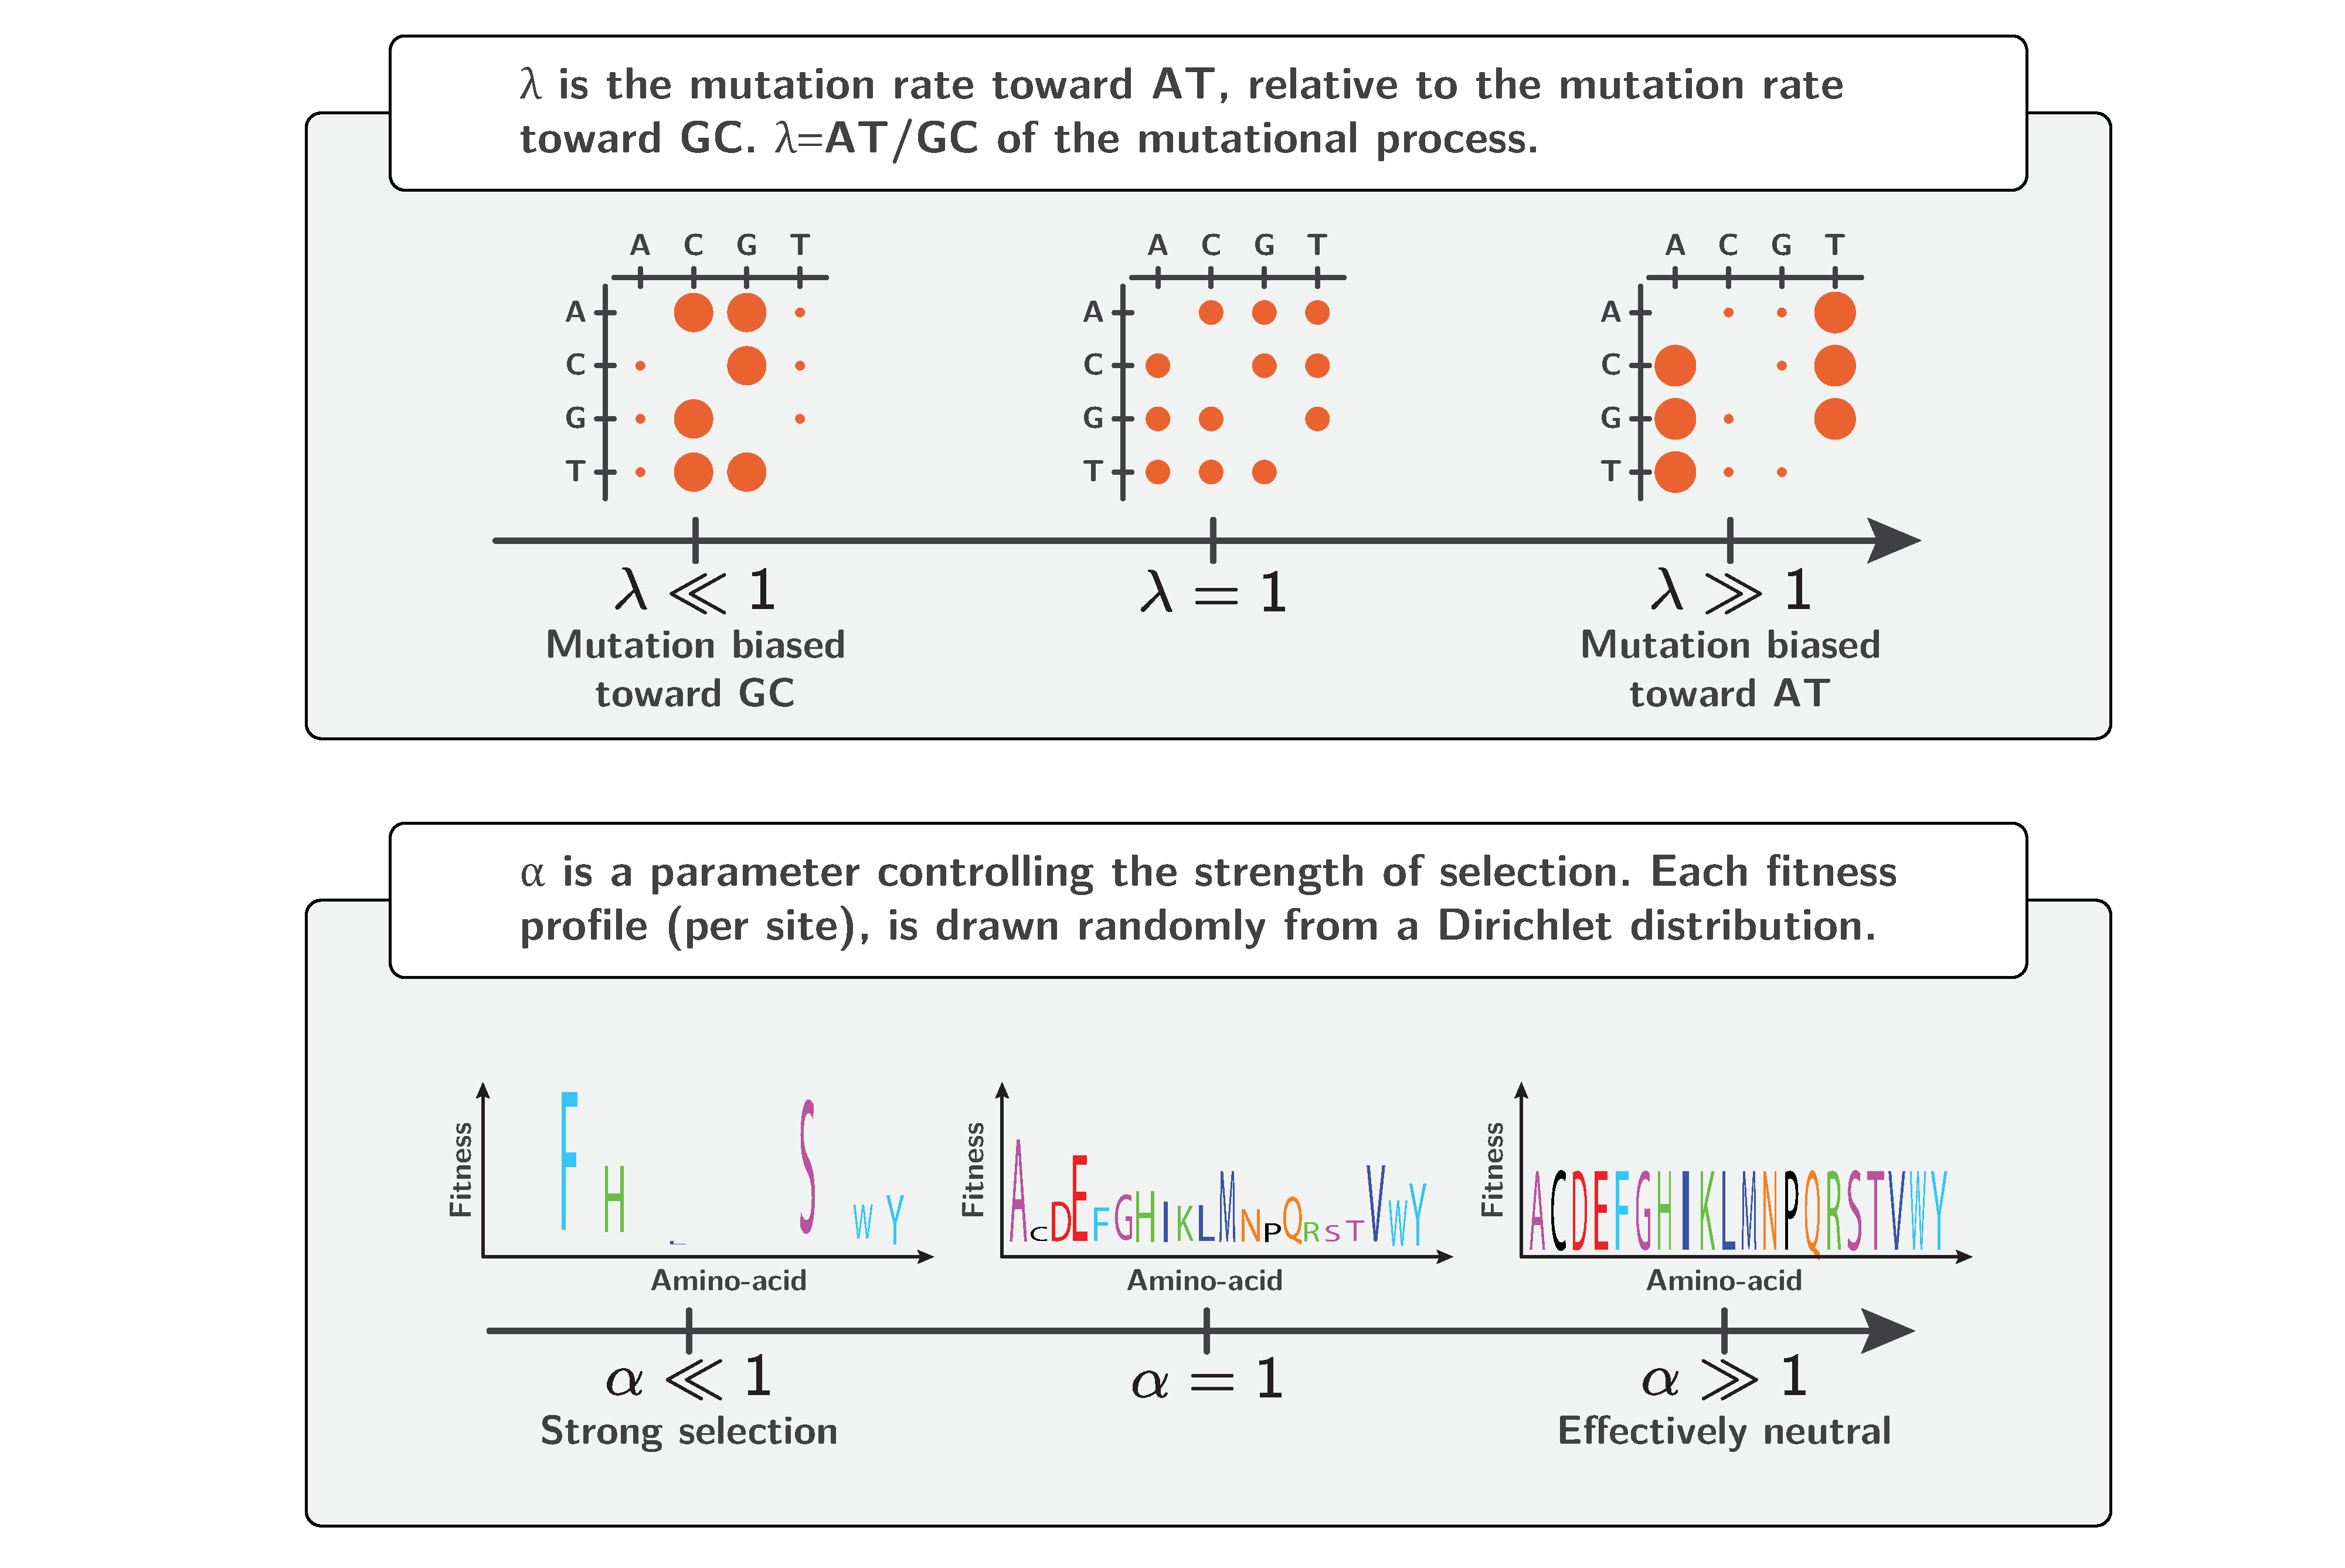
\includegraphics[width=\textwidth] {parameters}
    \caption[Parameters of the mutation-selection model]{
    Parameters of the mutation-selection model.
    Mutational bias (toward A and T) is shared by all sites of the sequence, and tuned by the parameter $\lambda$.
    Conversely, each codon site of the sequence is defined by a unique fitness profile, drawn from a Dirichlet distribution with concentration parameter $\alpha$.
    Stringency of selection increase with decreasing $\alpha$.}
    \label{fig:mut-bias-parameters}
\end{figure}

Simulation of this origin-fixation process along a species tree result in a multiple sequence alignment of \acrshort{DNA} for the extant species (see section~\ref{sec:mut-bias-simu}), from which summary statistics can be computed.
One such straightforward summary statistic is the frequency of the different nucleotides, and the resulting observed mutational bias $\atgc$ of the alignment.
Such observed mutational bias is compared to underlying mutational bias $\lambda$ at different positions of the codon (first, second and third), shown in figure~\ref{fig:mut-bias-AT-GC-obs}.
The third position of codons reflects the underlying mutational bias, while the first and second positions are impacted by the strength of selection and display less extreme bias than the underlying mutational bias.
This effect is explained by nucleotide mutations at the third codon position being more often synonymous, while mutations at first and second positions are more often changing the amino-acid and are more prone to selection.

\begin{figure}[htbp]
    \centering
    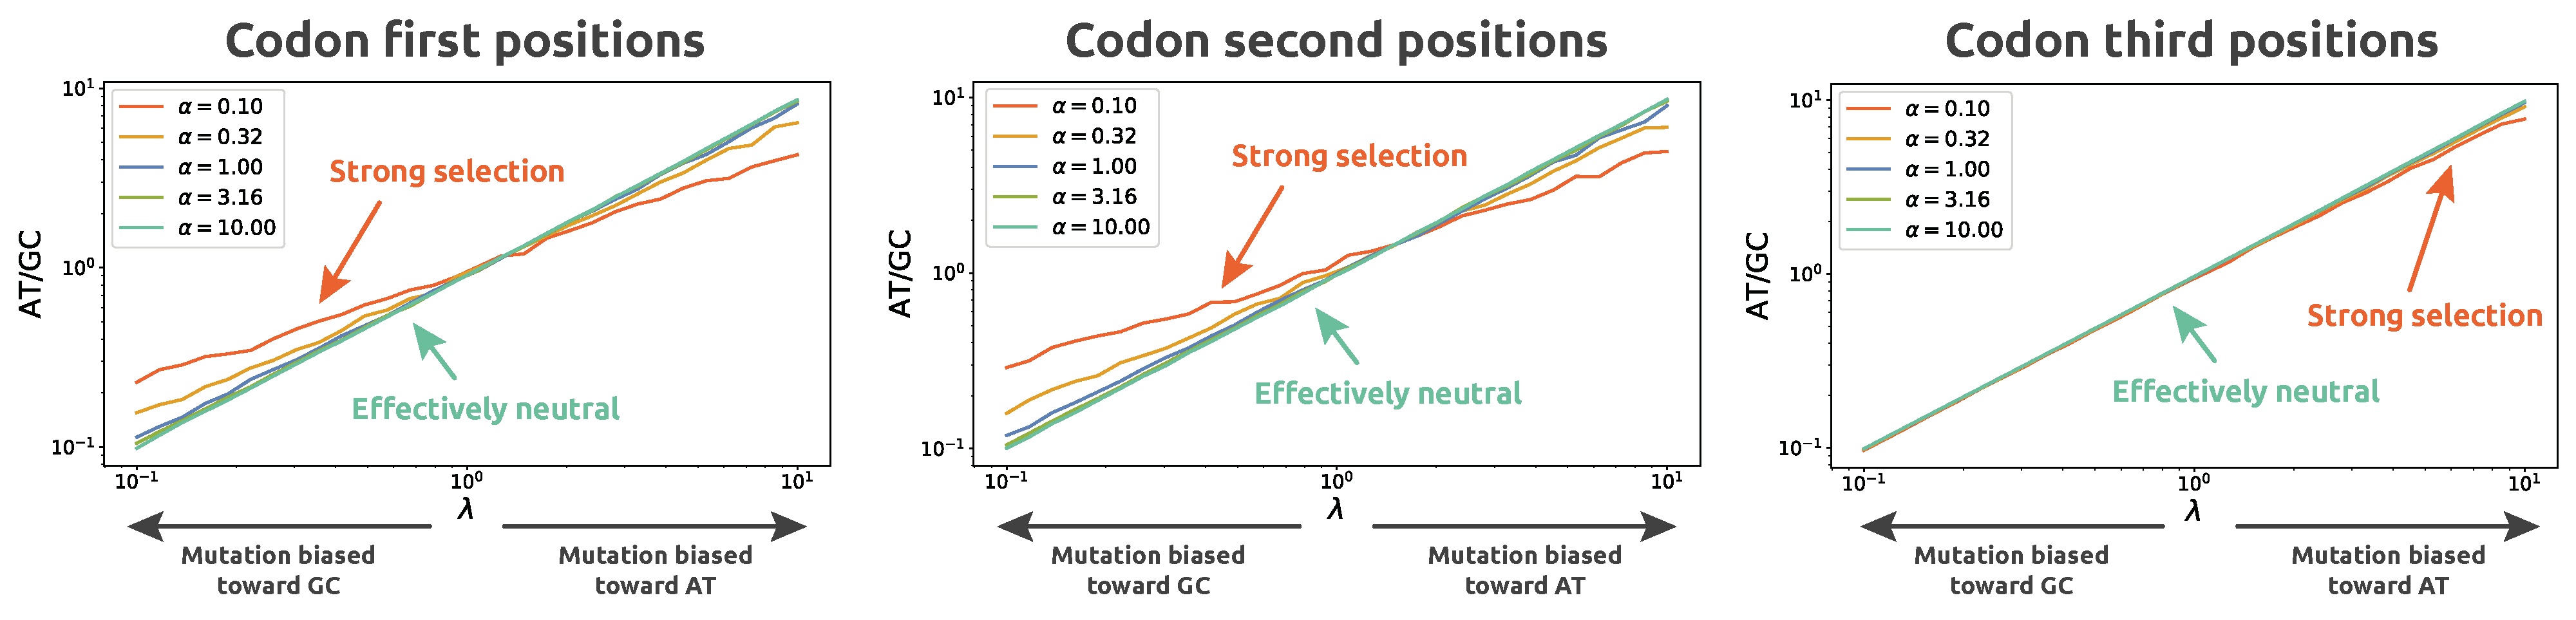
\includegraphics[width=\textwidth] {AT-GC-obs}
    \caption[$\atgc$ composition of the alignment]{
    Observed $\atgc$ composition of the alignment, represented at the different positions of codons (first, second and third), summed over all sites.
    The horizontal axis represents the underlying mutational bias ($\lambda$) of the nucleotide matrix, and the vertical axis represent the observed $\atgc$ of the codon position across the alignment.
    Stringency of selection is represented by 5 coloured solid lines with decreasing $\alpha$.
    $\atgc$ at the third codon position matches the mutational bias, whereas in contrast first and second positions are less extreme than the underlying bias.
    With increase stringency of selection (i.e. with decreasing $\alpha$), the observed bias is less reflecting the underlying mutational bias such that selection is opposing the mutational bias.}
    \label{fig:mut-bias-AT-GC-obs}
\end{figure}

Beside the observed mutational bias of the alignment, the diversity of amino acids is an important indicator of the selective constraints that the sequence experiences.
This diversity is quantified by the frequencies of amino acids observed across all taxa in the alignment, summarized through a single statistic, namely the Shannon's entropy of amino-acid frequencies~\citep{Goldstein2017}, as described in section~\ref{subsec:entropy}.
Diversity can be quantified for a given site of the sequence, and this site-specific diversity can subsequently be averaged over all sites of the sequence.
Alternatively, the diversity can be quantified directly on the whole sequence by the observed amino-acid frequencies in the alignment.
These two variants of diversity are computed for alignment under different values of $\alpha$ and $\lambda$, presented in figure~\ref{fig:mut-bias-diversity-aa}.
Under stringent selection, only a small number of amino acids are actually permissible any given site resulting in low site-specific diversity.
Yet all amino acids occur at comparable frequencies in the alignment resulting in high sequence diversity.
These observations highlight the distinction between averaged site-specific diversity and sequence diversity.
Moreover, the mutational bias (either toward AT or toward GC) greatly reduces both site-specific and sequence diversity, such that the composition of amino acids is highly dependent on the underlying mutational bias.
This effect is less visible whenever selection is more stringent (i.e. with decreasing $\alpha$), but can still be observed even for stringent selection.

\begin{figure}[htbp]
    \centering
    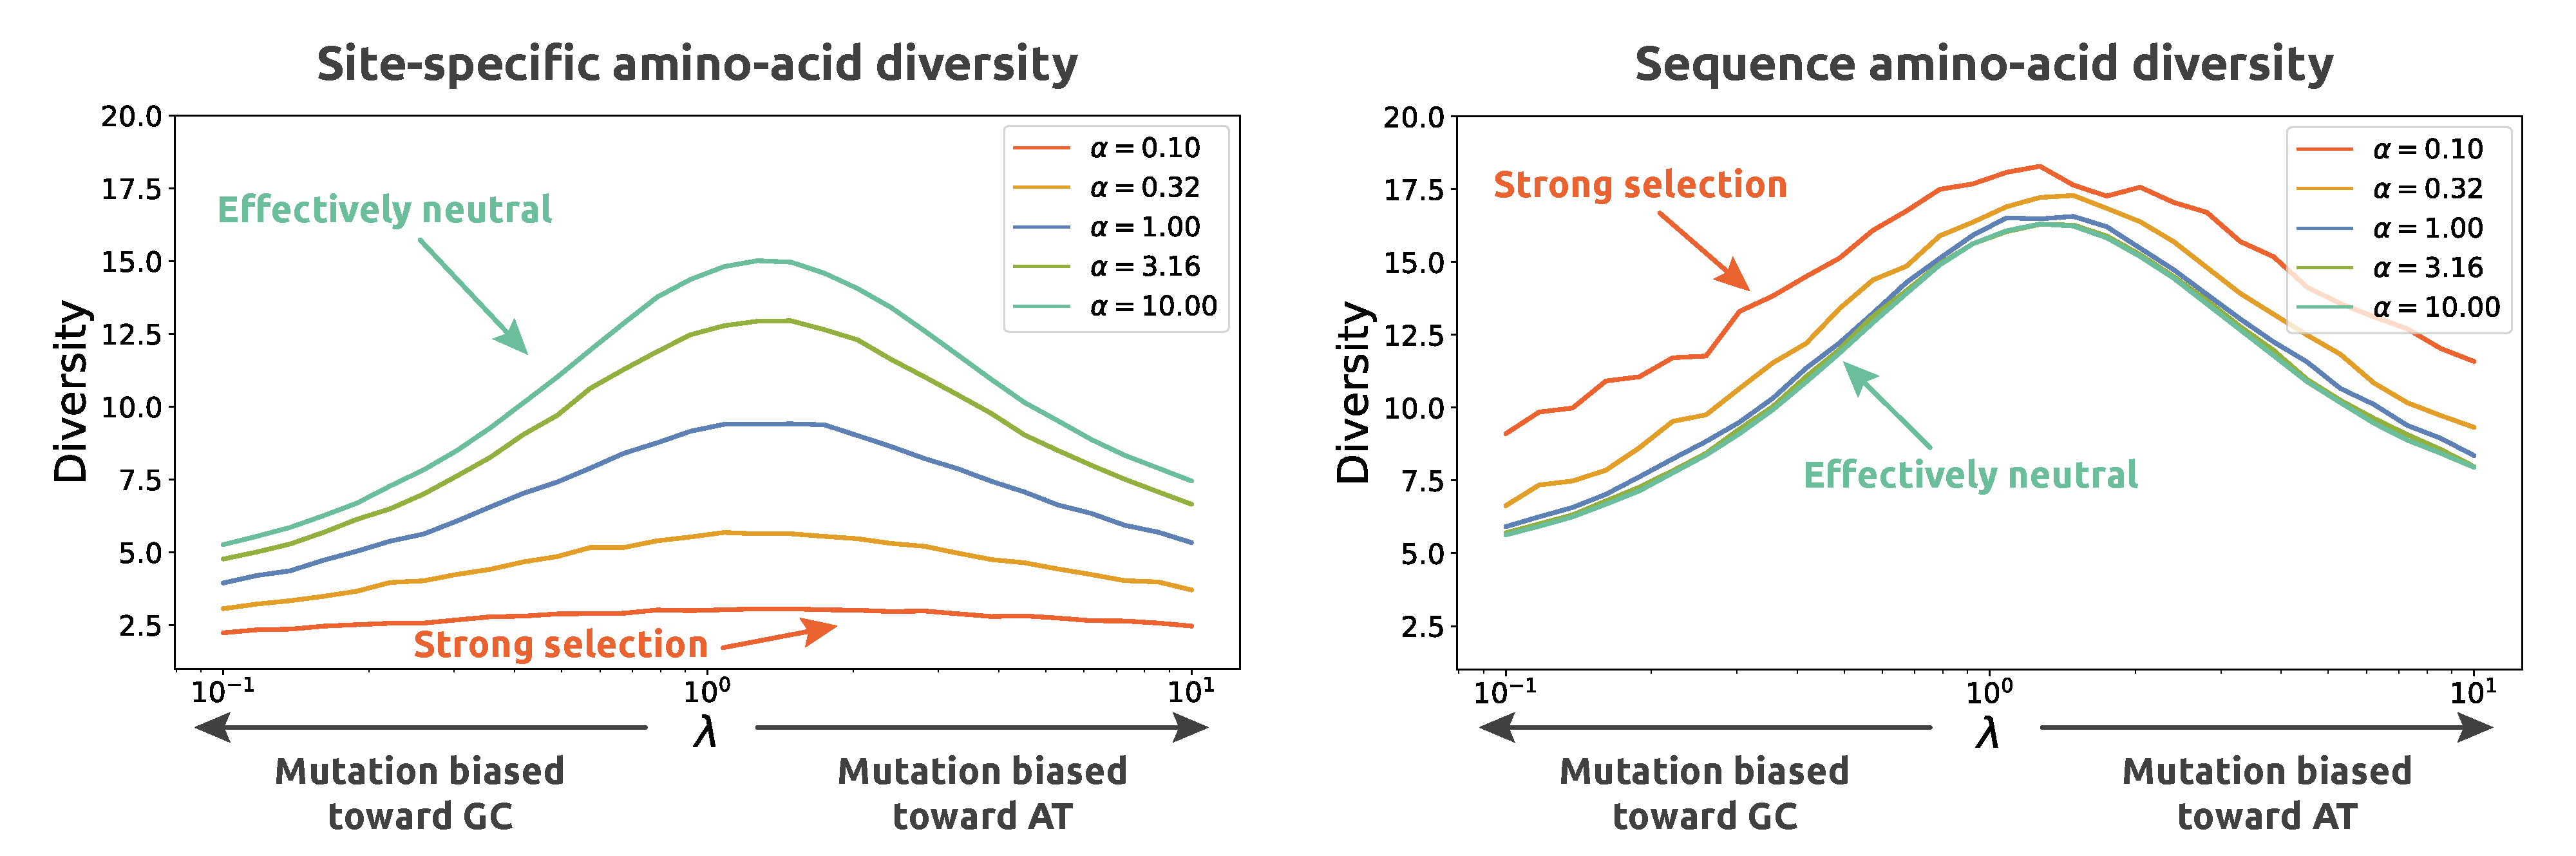
\includegraphics[width=\textwidth] {diversity-aa}
    \caption[Diversity of amino acids]{
    Diversity of the amino-acid frequencies is quantified as the exponential of Shannon's entropy in the vertical axis, either as site-specific diversity in the left panel or as sequence diversity in the right panel.
    Sequence diversity is higher than site-specific diversity, because at any given site only a small number of amino acids are actually permissible.
    From a selective perspective, site-specific diversity decreases with stringency of selection (decreasing $\alpha$ represented by 5 different solid lines) because at given site only a few amino acids are permitted.
    Conversely, because site-specific fitness profiles are randomly drawn, each site has different permitted amino acid, increasing the sequence diversity as the stringency of selection increases.
    From a mutational perspective, diversity decreases with increased mutational bias toward either toward AT or GC ($\lambda$ in horizontal axis).
    This effect is explained by the high frequency of amino acids containing nucleotides favoured by the underlying mutational bias.
    Finally, under stringent selection, diversity is less sensitive to the underlying mutational bias.}
    \label{fig:mut-bias-diversity-aa}
\end{figure}

%Evolutionary rate, which measures the rate at which mutations at individual sites arise and go to fixation, is governed by the amino acid distribution of individual sites, not the average distribution over a broad class of sites.
%The substitution rate (e.g., Grishin, Wolf \& Koonin, 2000).
%These two measures of evolutionary variability are considered to be essentially equivalent~\citep{Halpern1998}, though they are differently influenced by the mutational process~\citep{Santos2018}.

However, the diversity obtained from the observed alignment is biased by phylogenetic inertia, since the sequences are not independent of each other but related by a specie tree.
In addition, the observed diversity does not relate directly to the fixation probability of proposed mutations.
Instead, the mean scaled fixation probability of non-synonymous mutations ($\avgpfix$), which measures the rate at which mutations arise and go to fixation relatively to neutral mutation, is an aggregate parameter measuring the overall strength of selection throughout the process.
Moreover, $\avgpfix$ can be quantified from the substitutions recorded along the simulation (see section~\ref{subsec:fixation-bias}).
This parameter identifies with the ratio of non-synonymous over synonymous substitution rates, often called $\omega$ or $\dnds$~\citep{Spielman2015, DosReis2015, Jones2016}.
As expected, $\avgpfix$ is always lower than $1$ for simulation under a time-independent fitness landscape~\citep{Spielman2015}, and depends strongly on the stringency of selection ($\alpha$) as depicted in left panel of figure~\ref{fig:mut-bias-omega-WS}.
However, $\avgpfix$ depends weakly on the mutational bias ($\lambda$), contrarily the diversity highly dependent on $\lambda$.

This proxy of selection concerns all non-synonymous mutations, but we can consider the mean scaled fixation probability only for the subset of non-synonymous mutations from weak nucleotides (A or T) to strong nucleotides (G or C), called $\avgpfix_{\ATtoGC}$.
In this context, $\avgpfix_{\ATtoGC}$) increases in response to stronger mutational bias toward AT (i.e. with increasing $\lambda$), which had pushed codon containing favoured nucleotides toward less fit amino acid, as seen in the right panel of figure~\ref{fig:mut-bias-omega-WS}.
This distortion of selective effects toward GC is stronger with increased stringency of selection (i.e. with decreasing $\alpha$) .
Altogether, fixation probabilities are opposed to mutational bias, where the sequence is at an equilibrium point between these two forces.

\begin{figure}[htbp]
    \centering
    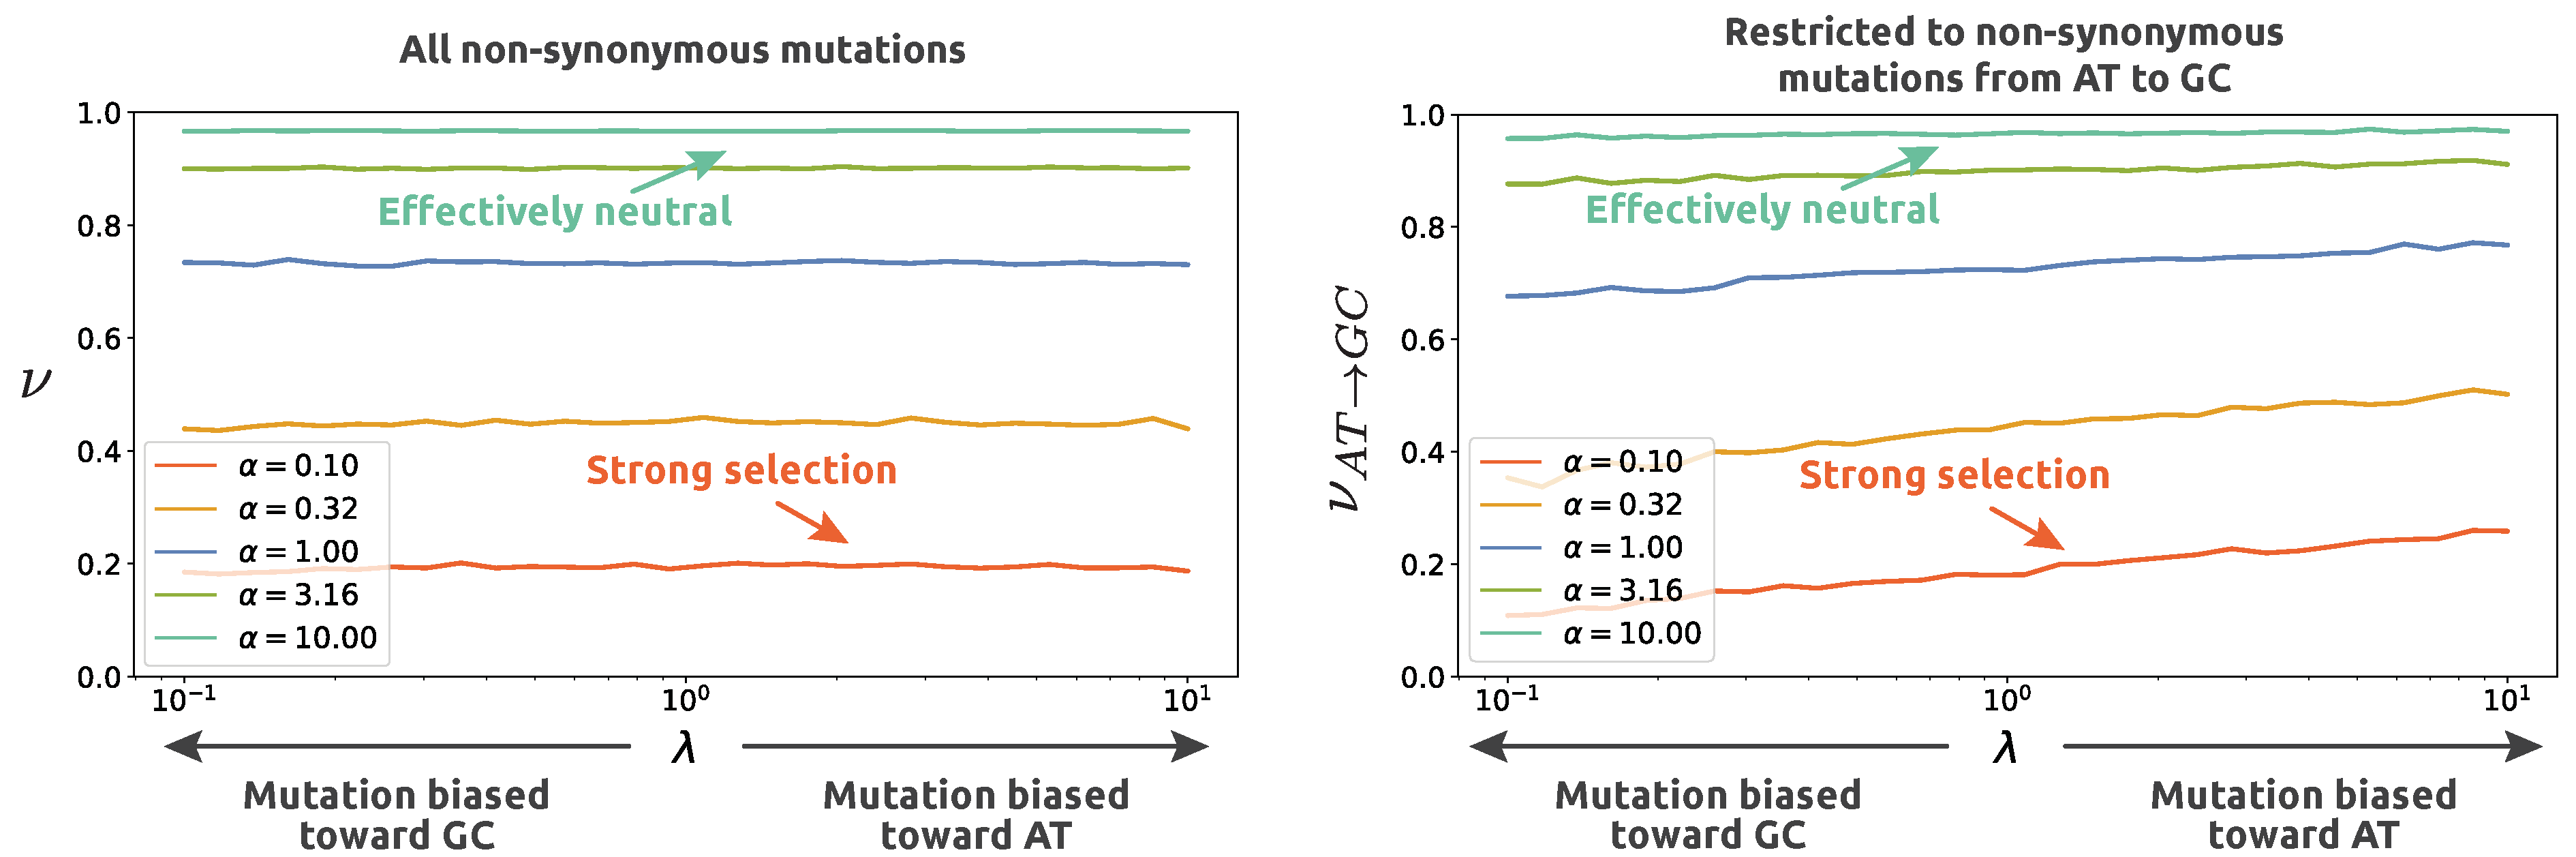
\includegraphics[width=\textwidth] {omega-AT-to-GC}
    \caption[Mean scaled fixation probability as a function of the parameters]{
    Mean scaled fixation probability ($\avgpfix$) in vertical axis as a function of mutational bias ($\lambda$) in the horizontal axis, for different stringency of selection ($\alpha$) in coloured solid lines.
    In the left panel, expectedly, $\avgpfix$ decrease with increased strength of selection (i.e. with decreasing $\alpha$).
    However, $\avgpfix$ is relatively unaffected by the mutational bias ($\lambda$).
    In the right panel, the mean scaled fixation probability of non-synonymous mutations is restricted to mutations from weak nucleotides (AT) to strong nucleotides (GC), called $\avgpfix_{\ATtoGC}$, represented in the vertical axis.
    A mutational process biased towards AT leads to an increased fixation probability toward GG, in the opposite direction.
    More generally, mutation bias is balanced by selection, where this effect increases with the stringency of selection.
    }
    \label{fig:mut-bias-omega-WS}
\end{figure}

\subsection{Parameter inference on simulated data}
\label{subsec:parameter-inference-on-simulated-data}

From an alignment of protein-coding \acrshort{DNA} sequences, without knowing the specific history of substitutions, estimates obtained with models of inference can approximate the mutational bias ($\lambda$) and the mean scaled fixation probability ($\avgpfix$).
Once the model is fitted to the data, the estimated parameters ($\widehat{\lambda}$, $\widehat{\avgpfix}$) can be compared to the known value of the simulation, as shown in figure~\ref{fig:mut-bias-pipeline}.

Practically, the likelihood of the data is computed from the tree topology and the instantaneous rates between codons, known as the 61x61 codon substitution matrix ($\Submatrix$).
Here we developed two models of inference, differing only by their parametrization of the codon matrix $\Submatrix$, considered homogeneous along the sequence (not site-specific).
Two models of inference are proposed, the first is based on \citet{Muse1994} formalism, and the second is based on a tensor of mean scaled fixation probabilities introduced in this study.

\begin{figure}[htbp]
    \centering
    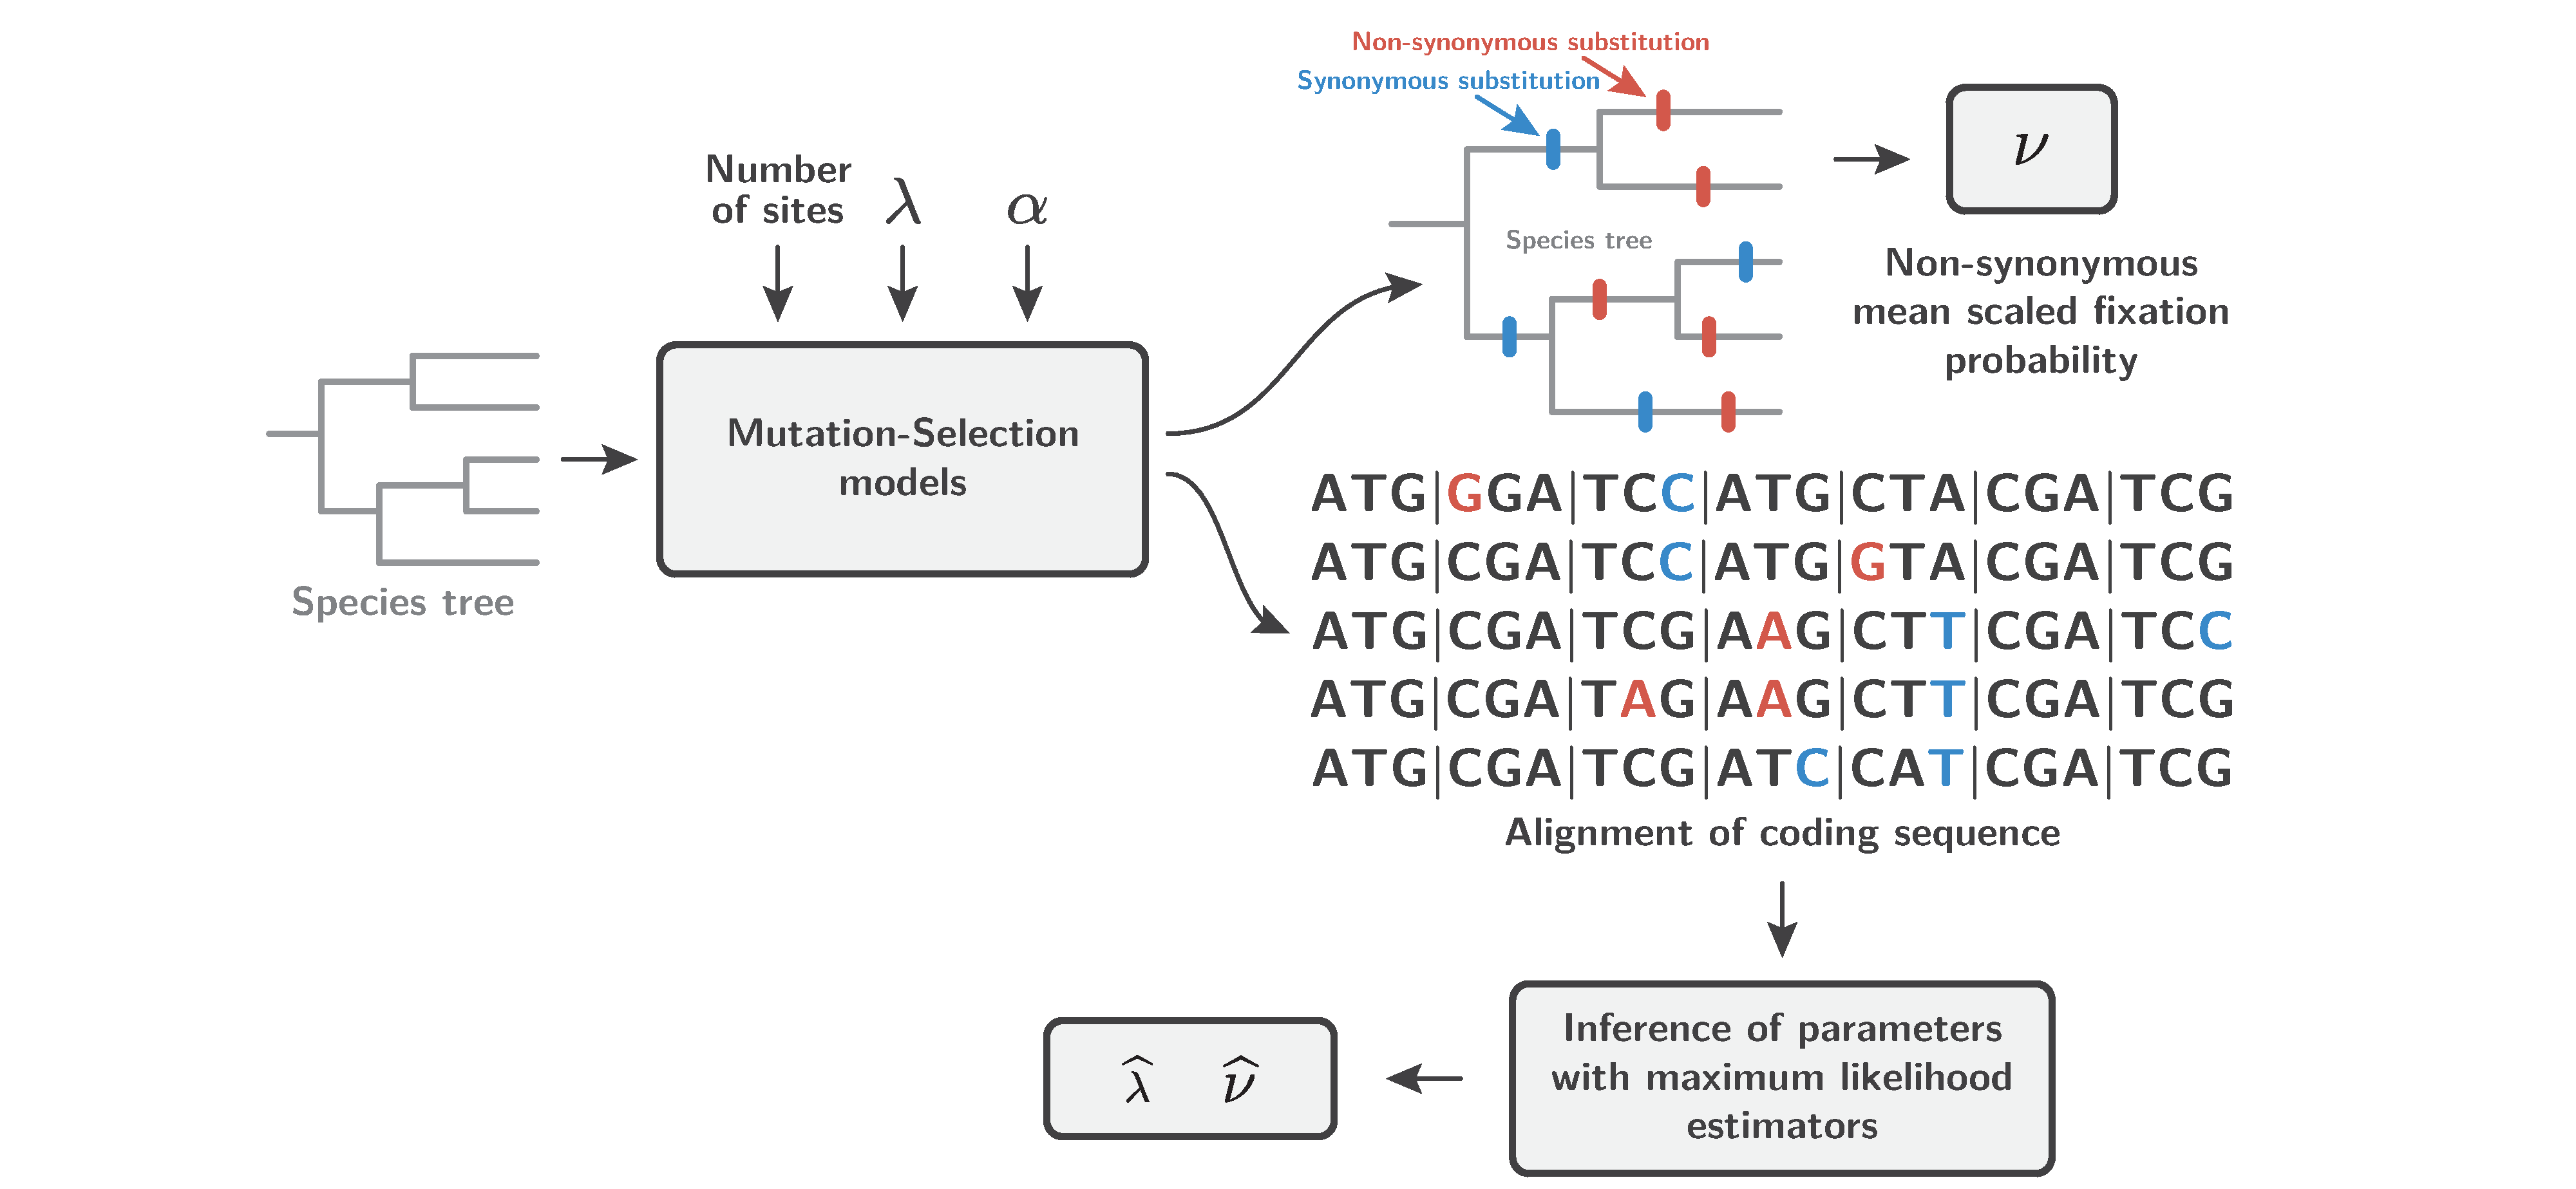
\includegraphics[width=\textwidth, page=1] {pipeline}
    \caption[Inferred value compared to known value]{
    Inferred value ($\widehat{\lambda}$, $\widehat{\avgpfix}$) compared to underlying value ($\lambda$, $\avgpfix$) of the simulation.
    The different parameterization of the inference model can result in different estimates of mutational bias ($\widehat{\lambda}$) and mean scaled fixation probability ($\widehat{\avgpfix}$).
    The main goal is to derive model of inference that can reliably estimate these parameters.
    Two models of inference are proposed, the first is based on Muse \& Gaut formalism, and the second based on a tensor of mean scaled fixation probabilities.}
    \label{fig:mut-bias-pipeline}
\end{figure}

\subsubsection{\texorpdfstring{$\omega$}{ω} as a scalar with Muse \& Gaut formalism}
At the level of nucleotides, the mutation rate is defined entirely by a generalized time-reversible nucleotide mutation rate matrix $\Mutmatrix$, which is a function of the nucleotide frequencies $\Mutequi$ and the symmetric exchangeability rates $\Exchan$~\citep{Tavare1986}:
\begin{equation}
    \mutmatrix_{a, b} = \exchan_{a,b}\mutequi_b
\end{equation}
At the level of codons, the substitution rate between the source ($\ci$) and target codon ($\cj$) depends on the underlying nucleotide change between ($\nucitoj$) and whether or not the change is non-synonymous.
Altogether, the substitution rates between codons $\submatrix_{\itoj}$, formalized by \citet{Muse1994} are a function of the mutation matrix $\Mutmatrix(\Mutequi, \Exchan)$, a single parameter of selective strength $\omega$, and the genetic code as:
\begin{equation}
    \begin{dcases}
        \submatrix_{\itoj} & = 0 \text{ if codons $\ci$ and $\cj$ are more than one mutation away,} \\
        \submatrix_{\itoj} & = \mutmatrix_{\nucitoj} \text{ if codons $\ci$ and $\cj$ are synonymous,} \\
        \submatrix_{\itoj} & = \omega \mutmatrix_{\nucitoj} \text{ if codons $\ci$ and $\cj$ are non-synonymous}.
    \end{dcases}
    \label{eq:codon-muse-gaut}
\end{equation}

Phenomenological codon models are not designed to tease out mutational bias, but firstly to estimate the global strength of selection ($\omega$).
From the maximum likelihood estimates of the \acrshort{GTR} mutation matrix ($\widehat{\Mutmatrix}$), we can estimate of the mutational bias toward $\text{AT}$ as $\widehat{\lambda}_{\text{MG}} = (\widehat{\mutequi_A} +\widehat{\mutequi_T}) /(\widehat{\mutequi_G} +\widehat{\mutequi_C}) $.
As shown in the left panel of figure~\ref{fig:mut-bias-inference}, estimate of the mutational bias is halfway between observed bias of the alignment and the true value used during the simulation.
As a result, this model cannot reliably infer the mutational bias, and is doing a compromise between estimating the selection coefficients and mutational bias.
We can also estimate the parameter ${\widehat{\omega}_{\text{MG}}}$, which is close to the underlying mean scaled fixation probability $\avgpfix$ computed during the simulation, with a precision of 98.2\%.

\subsubsection{\texorpdfstring{$\omega$}{ω} as a tensor with mean-field derivation}

Alternatively, gene-wide parameters of fixation should attempt to capture and aggregate site-specific parameterization of evolution.
As a result, projecting site-specific processes into a gene-wise process can be seen as a mean-field approximation, accounting for mean scaled fixation probability between amino acids, even though done at the level of the gene.

Because selection between codons reduces to selection between pairs of amino-acids, the mean-field approximation is parameterized by the mean scaled fixation probability between all pairs of amino acids, denoted $\omega_{\aaSource, \aaTarget}$.
For $20$ amino acids, the total number of pairs of amino acids is $190$, hence $380$ parameters by counting in both directions.
However, because of the structure of the genetic code, they are $75$ pairs that are one nucleotide away, since some amino acids are not directly accessible through a single non-synonymous mutation.
As a result, the number of parameters necessary to determine all mean scaled fixation probability ($\omega_{\aaSource, \aaTarget}$) in both directions is $150$.
However, under the assumption of a reversible process, the number of parameters can be reduced to the exchangeabilities $75$  ($\AAexchan_{\aaSource, \aaTarget}$) and $20$ the stationary distribution ($\AAequi_{\aaSource}$).
\begin{align}
    \omega_{\aaSource, \aaTarget} = \AAequi_{\aaTarget} \AAexchan_{\aaSource, \aaTarget}\text{, where } \AAexchan_{\aaSource, \aaTarget} = \AAexchan_{\aaTarget, \aaSource}.
\end{align}

Under projected mutation-selection model, the substitution rates between codons $\submatrix_{\itoj}$ are defined from a GTR mutation matrix $\Mutmatrix(\Mutequi, \Exchan)$, the selection coefficients $\UniDimArray{\omega}(\AAExchan, \AAEqui)$ and the genetic code:
\begin{equation}
    \begin{dcases}
        \submatrix_{\itoj} & = 0 \text{ if codons $\ci$ and $\cj$ are non neighbors}, \\
        \submatrix_{\itoj} & = \mutmatrix_{\nucitoj} \text{ if codons $\ci$ and $\cj$ are synonymous,}, \\
        \submatrix_{\itoj} & = \mutmatrix_{\nucitoj} \omega_{\aai, \aaj} \text{ if codons $\ci$ and $\cj$ are non-synonymous},
    \end{dcases}
    \label{eq:codon-mean-field}
\end{equation}
where $\aai$ is the amino acid encoded by codons $\ci$.

From the maximum likelihood estimates of the \acrshort{GTR} mutation matrix ($\widehat{\Mutmatrix}$), we can estimate the mutational bias $\left({\widehat{\lambda}_{\text{MF}}} \right)$ as previously.
As shown in the right panel of figure~\ref{fig:mut-bias-inference}, this model can tease out observed $\atgc$ of the alignment and the underlying mutational bias.
We can also estimate the mean scaled fixation probability of non-synonymous mutations $\widehat{\avgpfix}_{\text{MF}}$ (see section~\ref{sec:mut-bias-mean-field-omega}) which is a compound parameter of $\Mutmatrix(\Mutequi, \Exchan)$ and $\UniDimArray{\omega}$.
Under this model, $\widehat{\avgpfix}_{\text{MF}}$ is close to the $\avgpfix$ computed during the simulation, with a precision of 97.0\%.

\begin{figure}[htbp]
    \centering
    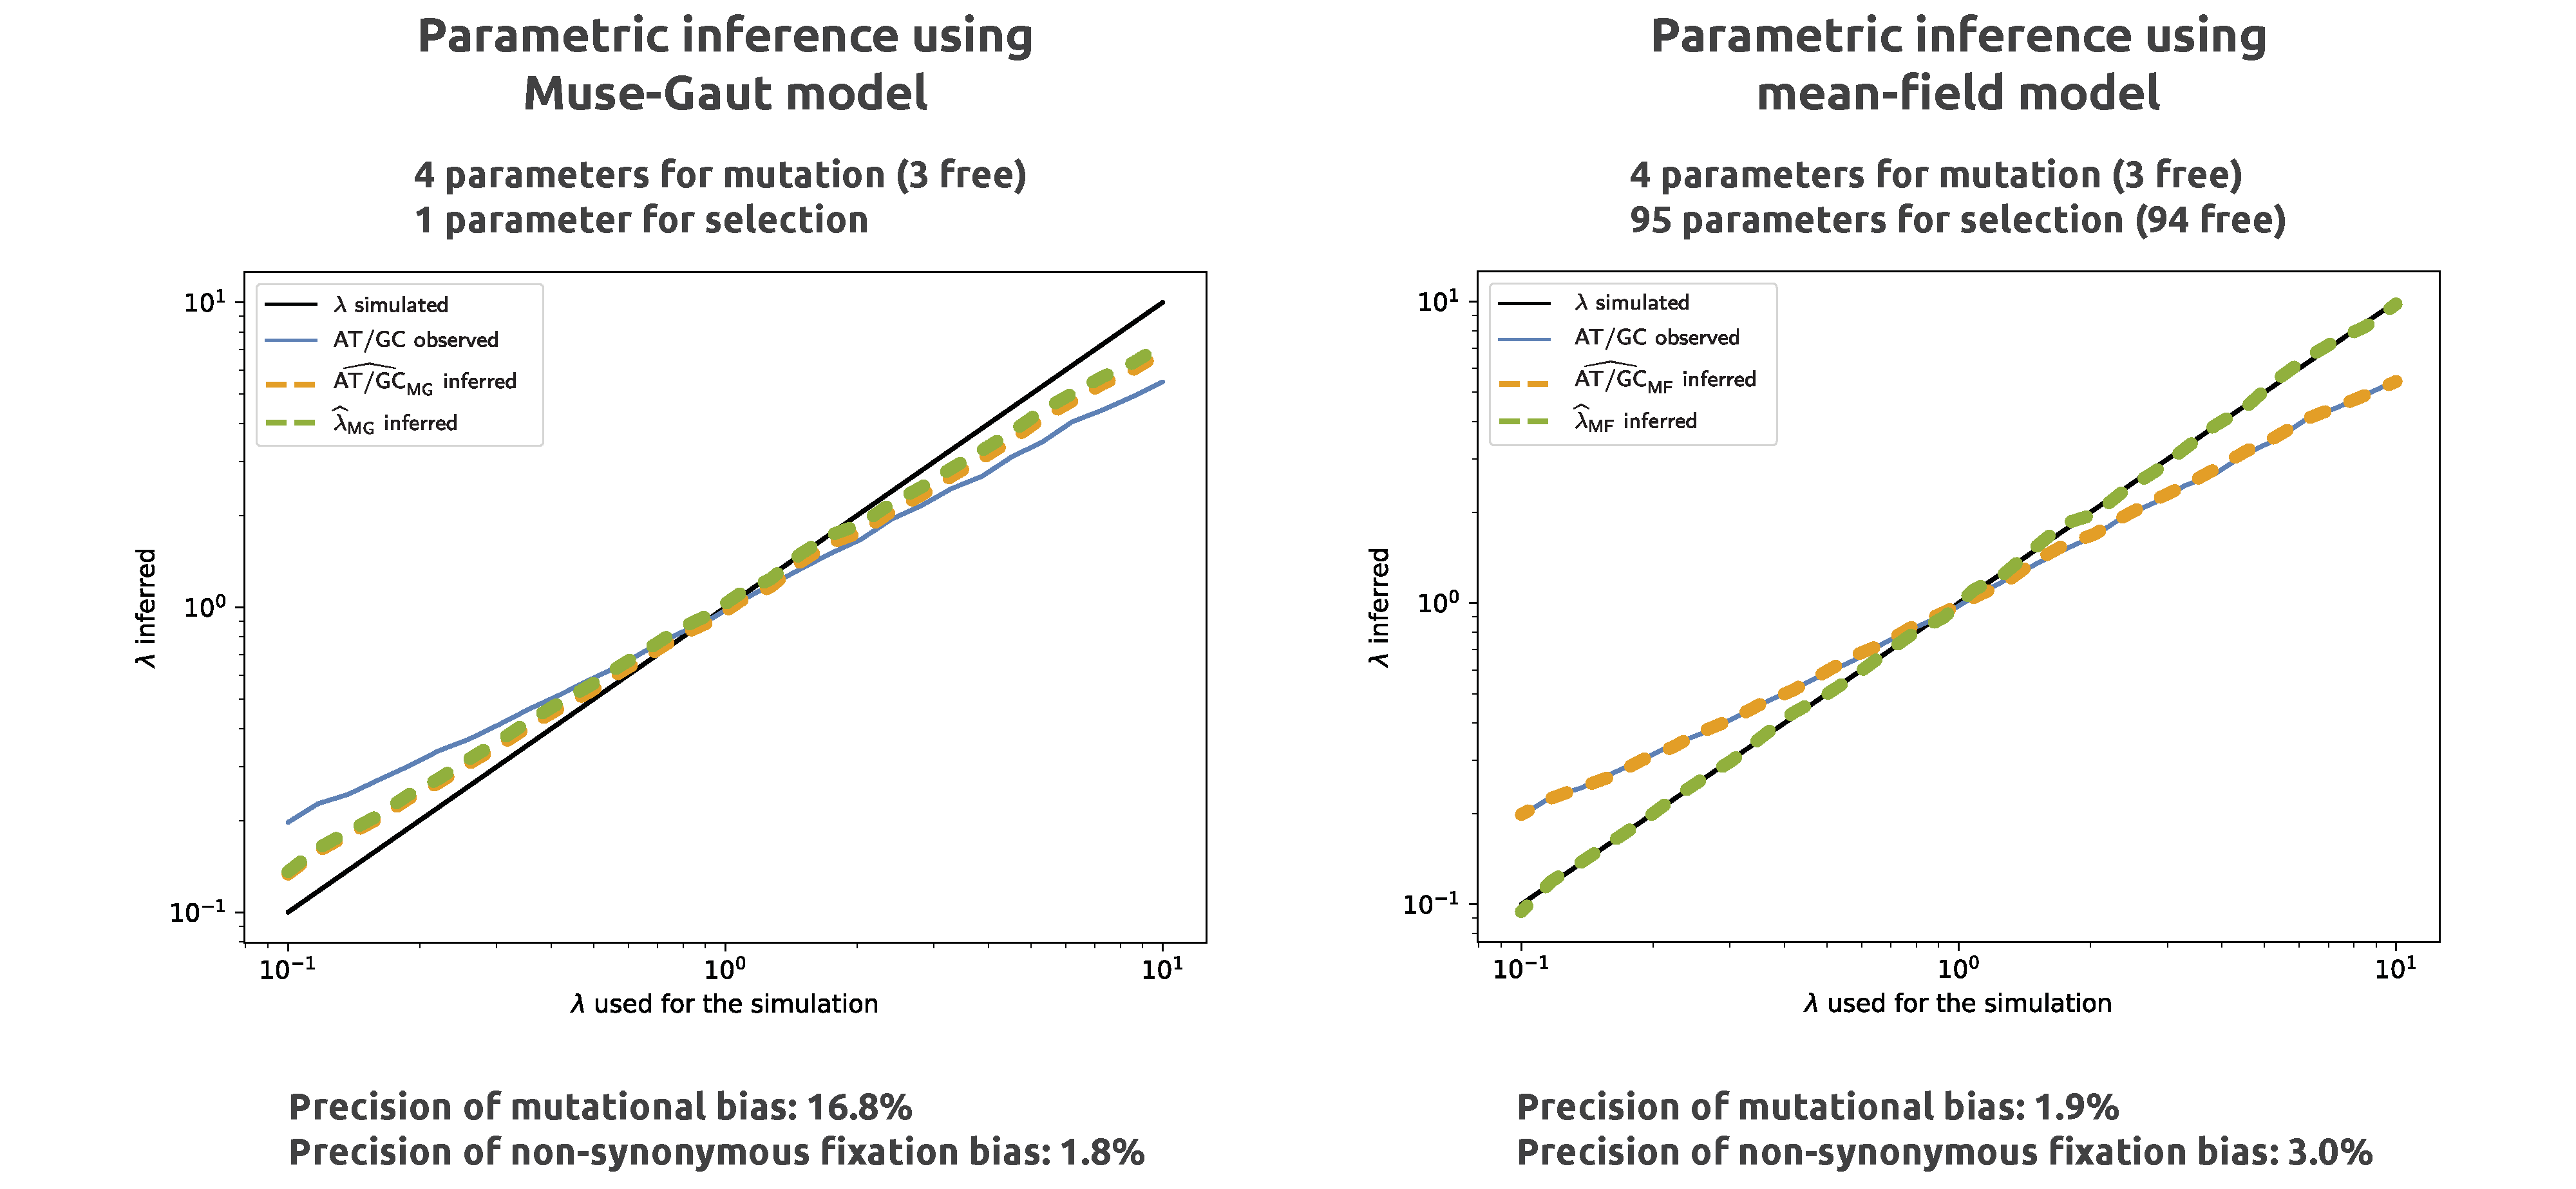
\includegraphics[width=\textwidth] {Simulation-vs-Inference}
    \caption[Estimation of mutational bias]{
    Different proxies of estimated mutational bias in the vertical axis are represented as a function of the underlying mutational bias ($\lambda$) of the simulation in the horizontal axis.
    Mutational bias can be estimated directly from the observed nucleotide frequencies in the alignment ($\atgc$ in blue solid line), similarly to figure~\ref{fig:mut-bias-AT-GC-obs}, which is skewed by selection and always less extreme than the underlying mutational bias.
    The robustness of mutational bias estimation of two different inference models are shown.
    Selection is modelled as a single $\omega$ parameter in the Muse \& Gaut formalism (MG) in the left panel, while selection is modelled as a tensor of $\omega$ parameters in different directions using a mean-field (MF) approximation in the right panel.
    In both panels, the true value of the mutational bias is represented in black solid line.
    The estimated mutational bias $\widehat{\omega}_{\text{MG}}$ (in yellow dotted line) in the MG formalism is between the true value and the observed $\atgc$.
    Conversely, estimated mutational bias $\widehat{\omega}_{\text{MG}}$ (in yellow dotted line) in the MF approximation equal to the underlying value.
    Moreover, the expected $\widehat{\atgc}$ from the parameter of the model fits the observed value in the MF approximation, while being skewed in the MG formalism.
    Altogether, the MF approximation can tease apart mutation and selection, while the MG formalism has to reach a compromise between observed $\atgc$ and underlying mutational bias.
    }
    \label{fig:mut-bias-inference}
\end{figure}

\subsection{Estimation of empirical sequence data}
\label{subsec:estimation-of-empirical-sequence-data}

The two implemented models of inference, namely classical Muse \& Gaut (MG) and mean-field (MF) are also applied to empirical protein-coding DNA alignment of nucleoprotein \& lactamase found in \citet{Bloom2017}, as shown in table~\ref{tab:mut-bias-estimation}.

The nucleoprotein alignment of 498 amino acids is available for 180 species, and is globally biased toward AT.
Similarly to our simulation, underlying mutational bias estimated with codon models is greater than this observation (i.e $1 < \atgc < \widehat{\lambda}$).
This effect is as previously due to selection at the level of amino acids concealing mutational bias in the alignment.
Moreover, the mutational bias estimated by the MF model is more extreme than the MG estimate (i.e. $1 < \widehat{\lambda}_{\text{MG}} < \widehat{\lambda}_{\text{MF}}$), also showing that MG is underestimating the underlying bias.
This example behaves identically to observation made with simulated alignments, where the MF model estimates a stronger mutational bias, which is supposedly closer to the real value.

Additionally, the estimated mean scaled fixation probability of non-synonymous mutations, denoted $\widehat{\avgpfix}_{\text{MF}}$, can be restricted to mutations from weak nucleotides (AT) to strong (GC), or vice versa (see section~\ref{sec:mut-bias-mean-field-omega}).
We observe that under a mutational bias favouring AT (i.e. $\lambda > 1$), the fixation probability non-synonymous mutations is higher toward GC than toward AT (i.e. $\widehat{\avgpfix}_{MF,\ATtoGC} > \widehat{\avgpfix}_{MF,\GCtoAT}$).

Reciprocally, for the gene lactamase, the alignment of 263 amino acids available for 85 species is globally biased toward GC.
Expectedly, the mean-field estimate is even more strongly biased toward GC (i.e $\widehat{\lambda}_{\text{MF}} < \atgc < 1$).
Curiously, the MG model estimates a weaker underlying mutational bias than the observed bias (i.e $ \atgc < \widehat{\lambda}_{\text{MG}} < 1$).
Likewise, we observe that under a mutational bias favouring GC (i.e. $\lambda < 1$), the fixation probability of non-synonymous mutations is higher toward AT than toward GC (i.e. $\widehat{\avgpfix}_{MF,\GCtoAT} > \widehat{\avgpfix}_{MF,\ATtoGC}$).

Altogether, empirical results are in agreement with observation on simulated results, namely that mutational bias results in skewed fixation probability of non-synonymous mutations opposing the mutational bias.
Our MF model estimates mutational bias more extreme than the MG model, and articulates mutation and selection such as to estimate reliably both mutation and selection.

\begin{table}[htbp]
    \centering
    \noindent\adjustbox{max width=\textwidth}{%
    \begin{tabu}{|c||c|c|}
        \hline
        \textbf{Estimated parameter} & Nucleoprotein & Lactamase \\
        \hline \textbf{$\atgc$ of the alignment} & 1.15 & 0.79 \\
        \hline \textbf{Muse \& Gaut mutational bias ($\widehat{\lambda}_{\text{MG}}$)} & 1.39 & 0.85 \\
        \hline \textbf{Mean-field mutational bias ($\widehat{\lambda}_{\text{MF}}$)} & 1.64 & 0.68 \\
        \hline \textbf{Mean-field scaled fixation probability from AT to GC ($\widehat{\avgpfix}_{MF,\ATtoGC}$)} & 0.14 & 0.31 \\
        \hline \textbf{Mean-field scaled fixation probability from GC to AT ($\widehat{\avgpfix}_{MF,\GCtoAT}$)} & 0.10 & 0.44 \\
        \hline
    \end{tabu}}
    \caption[Estimated parameters]{
    Estimated parameters of mutational bias ($\widehat{\lambda}$) from two models of inference, namely classical Muse \& Gaut (MG) and mean-field (MF).
    These models are applied to two distinct datasets of protein-coding DNA alignment, nucleoprotein in the left column and lactamase in the right column.
    By taking into account selection in multiple direction, MG models estimates stronger mutational bias than the MG model.
    For the MG model the mean scaled fixation probability of non-synonymous mutations ($\widehat{\avgpfix}_{MF}$) can be obtained either from weak (AT) to strong nucleotides (GC), or vice versa.
    The fixation probability of non-synonymous mutations is opposed to the underlying mutational bias, such that a skewed mutational process results in a skewed selection, justifying that they must be articulated together.
    }
    \label{tab:mut-bias-estimation}
\end{table}


\section{Discussion}\label{sec:discussion}

The observed composition of \acrshort{DNA} sequences is the result of the interplay between mutation and selection, such that the observed mutational bias in the alignment is different to the underlying mutational bias.
In protein-coding \acrshort{DNA} sequences, the nucleic composition result in the subtle interplay between mutation at the nucleic level and selection at the protein level.
Unfortunately, parametric codon models are inherently misspecified to untangle mutation and selection, and they don't estimate the mutational process reliably.

In this work we seek to find the simplest parametric codon model able to correctly tease apart mutation rates on one hand, and net mean fixation probabilities without having to explicitly model the underlying fitness landscape.
In order to derive a codon model along those lines, our strategy is to first assume an underlying site-specific, time-independent fitness landscape.
Then, we derive the gene-wise mean fixation probabilities between all pairs of codons, implied across all sites by the underlying process.
Finally, we observe that this mean-field process should in fact invoke as many distinct $\omega$ parameters as there are pairs of amino acids that are nearest neighbours in the genetic code.
There are reversibility conditions, reducing the dimensionality and allowing for a GTR-like parameterization of this tensor ($95$ parameters for selection).

Inferring parameters on simulated alignments, we show that the model correctly estimates the underlying mutational bias and selective pressure.
Applied to empirical alignments, we also observed that there is a selective pressure for certain amino acids opposed to the underlying mutational bias, justifying that selection and mutation must be articulated together.

This work first points to a fundamental behaviour of molecular sequences, namely that they are not optimized but are the result of an equilibrium between forces.
In the specific case highlighted in this work, mutational bias at the nucleotide-level results in suboptimal amino-acid being overrepresented in the sequence, leading to selection favouring amino acids that were underrepresented.
As an example of this pervasive effect, observed selective effect toward GC is mimicking biased gene conversion toward GC (\acrshort{gBGC}).
As a result, experiments observing fixation bias toward GC must also rule out that this fixation bias is not an artefact or byproduct of an underlying mutational bias toward AT.
Altogether, our observations and modelling principles offers tools to better understand how mutation-mutation will work together with biased gene conversion (\acrshort{gBGC}), and therefore also yields better understanding of how \acrshort{gBGC} will impact both nucleotide composition and $\dnds$.
It worth mentioning that in our result focused on the fixation probability from AT to GC ($\widehat{\avgpfix}_{\ATtoGC}$) because of the relationship to gBGC, while in practice, the same analysis and methods can be applied to any subset of nucleotides or codons.

Our mean-field parametric model use gene-wise parameters of mean scaled fixation probabilities, and even though the underlying selective landscape is site-specific, such approximation can nonetheless be used to disentangle mutation and selection.
As a result, this study demonstrates that phenomenological models derived out of mechanistic models are more compact (i.e. not site-specific), and in certain cases are sufficient to extract relevant parameters.
This methodology for deriving inference models is done in two steps, first assuming an underlying mechanistic model of sequence evolution, parameterized by variables that are derived from first principles (fitness landscape, mutations rates, $\hdots$).
Subsequently, the phenomenological inference model is obtained by matching aggregate parameters derived out of the mechanistic model.
Altogether, inference model can be phenomenological in practice, but should nonetheless be derived for mechanistic models such as to articulate the interplay between, mutation, selection, drift and other evolutionary forces.

Finally, this work is preliminary result, and this model should be tested against a more diverse range of empirical data, in terms of phylogenetic depth, strength of selection, codon usage bias to assert for the validity of our empirical results.
Also, the empirical fit to the data between the models (e.g. using AIC) should be more carefully examined.
Indeed, by setting $\AAEqui = \vecOne$ and $\AAExchan = \omega \vecOne$ in our mean-field models, we retrieve the nested Muse \& Gaut model, hence both models are directly comparable.
In addition, several other codon models~\citep{Rodrigue2008a,KosakovskyPond2020} should be included in a broader comparison of estimation of underlying mutational bias and strength of selection on protein-coding DNA sequence.


\section{Materials \& Methods}

\subsection{Simulation model}
\label{sec:mut-bias-simu}
We seek to simulate the evolution of protein-coding sequences along a specie tree.
Starting with one sequence at the root of the tree, the sequences evolves independently along the different branches of the tree by point substitutions, until they reach the leaves.
At the end of the simulation, we get one sequence for each leaf of the tree, meaning one sequence per specie.
Such evolutionary process is an idealized version of the reality, in the sense that the whole heterogeneity of sequences in the population is discarded, with only one sequence representing the whole population.
For a protein-coding \acrshort{DNA} sequence, a substitution is modelled as the product of mutation at the nucleotide level, and selection at the amino-acid level.

On one hand, the mutation rate between nucleotides as assumed to be shared by all sites of the sequences.
On the other hand, the selection for amino acids is assumed to be varying along the sequences.
During the simulation, from a given sequence, the substitution rate toward all possible mutant (one nucleotide change) is computed and the next substitution at the waiting time until such event is obtained by Gillespie's algorithm~\citep{Gillespie1977}.

\subsection{Mutational bias at the nucleotide level}
\label{sec:mut-bias-mut-matrix}
The mutation rate between nucleotides is always proportional to $\mu$.
Moreover, mutations from any nucleotide to another weak nucleotide is increased by the factor $\lambda$ compared with mutations to another strong nucleotide.
The rate at which a nucleotide doesn't change is given such as the sum of all rates is zero.
The mutation rate matrix is:
\begin{equation}
    \label{nucMatrix}
    \Mutmatrix =
    \begin{blockarray}{ccccc}
        & A & C & G & T \\
        \begin{block}{c(cccc)}
            A & {-\mu(2 + \lambda)} & {\mu} & {\mu} & {\mu \lambda} \\
            C & {\mu \lambda} & {-\mu(1 + 2\lambda)} & {\mu} & {\mu \lambda} \\
            G & {\mu \lambda} & {\mu} & {-\mu(1 + 2\lambda)} & {\mu \lambda} \\
            T & {\mu \lambda} & {\mu} & {\mu} & {-\mu(2 + \lambda)} \\
        \end{block}
    \end{blockarray}
\end{equation}
The stationary distribution $ \Subequi$ must be annihilated by the mutation matrix $\Mutmatrix$, which gives the stationary distribution:
\begin{align}
    \Mutequi \Mutmatrix & = \vecOne, \\
    \iff \Mutequi & = \left( \dfrac{\lambda}{2+2\lambda}, \dfrac{1}{2+2\lambda}, \dfrac{1}{2+2\lambda}, \dfrac{\lambda}{2+2\lambda} \right).
    \label{nucStationarity}
\end{align}
The process is reversible and fulfils detailed balance conditions for any pair of different nucleotides:
\begin{align}
    \mutequi_a \mutmatrix_{a, b} =\mutequi_b \mutmatrix_{b, a}.
    \label{nucMutBalance}
\end{align}
It is important to note that ratio of weak over strong nucleotides frequency at stationarity is equal to $\lambda$:
\begin{align}
    \label{lambda}
    \dfrac{ \mutequi_A + \mutequi_T }{ \mutequi_C + \mutequi_G }
    & = \dfrac{ \lambda ( 2 + 2 \lambda)^{-1} + \lambda ( 2 + 2 \lambda)^{-1}}{ ( 2 + 2 \lambda)^{-1} + ( 2 + 2 \lambda)^{-1}}, \ \text{from eq.~\ref{nucStationarity},}\\
    & = \lambda.
\end{align}

\subsection{Selection at the amino-acid level}
\label{sec:mut-bias-aa-selection}
The substitution rate is considered null if the pair of codons differs by more than one nucleotide.
Otherwise, the mutation rate between a pair of codons is given by the mutation rate of the underlying nucleotides.
We subsequently take into account the selection at the amino-acid level, where each amino acid $\aai$ encoded by codons $\ci$ are given a fitness ($\Fiti$).
By modelling fitness at the amino-acid level, we assume that all codons encoding for one particular amino acid are selectively neutral.
In this modelling framework, the genetic code is of particular importance since the number of codons encoding for a particular amino acid varies greatly.
As an example, tryptophan is encoded by one codon, while leucine is encoded by 6 codons.
Intuitively, this variation makes the mutation bias more pronounced in codons encoding for the same amino acids, since there are more mutations possible that are selectively neutral (i.e synonymous).
On the other hand, the mutation bias is more constrained if the amino acid is encoded by a few codons since there are only a few (or not any) synonymous mutations.

To take into account the heterogeneity of selection between different sites of the protein, we assume that each site $\site$ of the sequence is evolving under a different fitness landscape ($\Fiti\siteexp$).
At one particular site, under a time-independent fitness landscape, the substitution rate between codons is given by the product of the mutation rate and the probability of fixation:
\begin{equation}
    \begin{dcases}
        \submatrix_{\itoj}\siteexp & = 0 \text{ if codons $\ci$ and $\cj$ are more than one mutation away,}\\
        \submatrix_{\itoj}\siteexp & = \mutmatrix_{\nucitoj} \text{ if codons $\ci$ and $\cj$ are synonymous,} \\
        \submatrix_{\itoj}\siteexp & = \mutmatrix_{\nucitoj} \dfrac{\Fitj\siteexp - \Fiti\siteexp}{1 - \e^{\Fiti\siteexp - \Fitj\siteexp} } \text{ if codons $\ci$ and $\cj$ are non-synonymous}.
    \end{dcases}
    \label{eq:codonsubrates}
\end{equation}
At the root the tree, the sequence is obtained by sampling from the equilibrium stationary distribution.
The stationary distribution $\Subequi$ at site $\site$ can be obtained as:
\begin{align}
    \subequi_{\ci}\siteexp & = \mathcal{Z}\siteexp \left[\prod\limits_{k \in \{ 1, 2, 3 \}} \mutequi_{\ci[k]}\right] \e^{\Fiti\siteexp},
    \label{codonStationarity}
\end{align}
where $\ci[k]$ denotes the nucleotide at position $k \in \{ 1, 2, 3 \}$ of codon $i$, and $\mathcal{Z}\siteexp $ is the normalizing constant:
\begin{align}
    \mathcal{Z}\siteexp = \left( \sum\limits_{\cj=1}^{61} \left[\prod\limits_{k \in \{ 1, 2, 3 \}} \mutequi_{\cj[k]}\right] \e^{\Fitj\siteexp} \right)^{-1}
\end{align}
Moreover, the substitution process is reversible and fulfils detailed balance conditions at each site $\site$:
\begin{align}
    \subequi_{\ci}\siteexp \submatrix_{\itoj}\siteexp = \subequi_{\cj}\siteexp \submatrix_{\cj, \ci}\siteexp
    \label{codonSubBalance}
\end{align}

The next substitution event, and the time to reach such event is chosen using Gillespie's algorithm~\citep{Gillespie1977}, according to the rates of substitution ($\submatrix_{\itoj}$) between sequences.

\subsection{Diversity of amino-frequencies}
\label{subsec:entropy}

For a site $\site$, the diversity $D\siteexp$ is computed as the exponential of Shannon's entropy from the frequencies of the different amino-acids ($\profile\siteexp$):
\begin{equation}
    D(\profile\siteexp) = \exp \left[ - \sum\limits_{\SetAa} \profile\siteexp_{\aminoacid} \ln \left( \profile\siteexp_{\aminoacid} \right) \right]
    \label{eq:diversity-site-specific}
\end{equation}
The diversity is a measure of the flatness of the fitness profile, with a value of $1$ corresponding to a single peak fitness landscape (i.e. with only one amino acid permissible), and a value of $20$ corresponding to a neutral landscape, where each amino acid has the same fitness.
The diversity can be averaged over all sites as:
\begin{equation}
    \left\langle D(\profile) \right\rangle = \dfrac{1}{\Nsite}\sum\limits_{\Setsite} D(\profile\siteexp)
    \label{eq:diversity-site-specific-avg}
\end{equation}
Otherwise, frequencies of the different amino-acids can first be averaged over all sites:
\begin{equation}
    \left\langle \profile \right\rangle = \dfrac{1}{\Nsite}\sum\limits_{\Setsite} \profile\siteexp
    \label{eq:profile-gene-wise}
\end{equation}
Then the gene-wise diversity is simply:
\begin{equation}
    D \left(  \left\langle \profile \right\rangle \right) = \exp \left[ - \sum\limits_{\SetAa} \left\langle \profile \right\rangle_{\aminoacid} \ln \left( \left\langle \profile \right\rangle_{\aminoacid} \right) \right]
    \label{eq:diversity-gene-wise}
\end{equation}

\subsection{Mean scaled fixation probability}
\label{subsec:fixation-bias}
The sequence at time $t$ is denoted $\Seqi(t)$ and the codon present at site $\site$ is denoted $\Seqi_{\site}(t)$.
For a given sequence, the mean scaled fixation probability of mutations is the ratio :
\begin{align}
    \avgpfix (t) & = \dfrac{ \sum\limits_{\site} \sum\limits_{\cj \in \NonSynNeighbors \left ( \Seqi_{\site}(t) \right)} Q_{\Seqi_{\site}(t) \to \cj}}{ \sum\limits_{\site} \sum\limits_{\left ( \cj \in \Seqi_{\site}(t) \right)} \mu_{\Seqi_{\site}(t) \to \cj}},
\end{align}
where $\setNonSynNeighbors$ is the set of non-synonymous codons neighbours of codon $\ci$ and $\submatrix_{\itoj}\siteexp$ are defined as in equation~\ref{eq:codonsubrates}.
Averaged over all branches of the tree, the mean scaled fixation probability is :
\begin{align}
    \avgpfix & = \left\langle \avgpfix (t) \right\rangle, \\
    & = \int_{t} \avgpfix (t) \der t,
\end{align}
where the integral is taken over all branches of the tree, while the integrand ($\avgpfix (t)$) is a piece-wise function changing after every point substitution event.

Moreover, mean scaled fixation probability from weak (AT) to strong (GC) nucleotides denoted $\avgpfix_{\ATtoGC}$ is obtained similarly by restricting the sums (in the numerator and the denominator) to one nucleotide mutations only from weak to strong.

\subsection{Derivation of mean-field model}
\label{subsec:mean-field-derivation}
The average fixation probability between codon $\ci$ and codon $\cj$ is given as:
\begin{align}
    \left\langle \avgpfix_{\itoj} \right\rangle & = \dfrac{ \left\langle \subequi_{\ci} 2\Ne \pfix(\itoj) \right\rangle }{ \left\langle \subequi_{\ci} \right\rangle }, \\
    & = \dfrac{ \sum\limits_{\site} \subequi_{\ci}\siteexp \dfrac{\Fitj\siteexp - \Fiti\siteexp}{1 - \e^{\Fiti\siteexp - \Fitj\siteexp}} }{ \sum\limits_{\site} \subequi_{\ci}\siteexp }, \\
    & = \dfrac{ \sum\limits_{\site} \mathcal{Z}\siteexp \left[\prod\limits_{k \in \{ 1, 2, 3 \}} \mutequi_{\ci[k]}\right] \e^{\Fiti\siteexp} \dfrac{\Fitj\siteexp - \Fiti\siteexp}{1 - \e^{\Fiti\siteexp - \Fitj\siteexp}} }{ \sum\limits_{\site} \mathcal{Z}\siteexp \left[\prod\limits_{k \in \{ 1, 2, 3 \}} \mutequi_{\ci[k]}\right] \e^{\Fiti\siteexp} }, \\
    & = \dfrac{ \left[\prod\limits_{k \in \{ 1, 2, 3 \}} \mutequi_{\ci[k]}\right] \sum\limits_{\site} \mathcal{Z}\siteexp  \dfrac{\Fitj\siteexp - \Fiti\siteexp}{ \e^{-\Fiti\siteexp} - \e^{ - \Fitj\siteexp}} }{ \left[\prod\limits_{k \in \{ 1, 2, 3 \}} \mutequi_{\ci[k]}\right] \sum\limits_{\site} \mathcal{Z}\siteexp \e^{\Fiti\siteexp} }, \\
    & = \dfrac{ \sum\limits_{\site} \mathcal{Z}\siteexp  \dfrac{\Fitj\siteexp - \Fiti\siteexp}{ \e^{-\Fiti\siteexp} - \e^{ - \Fitj\siteexp}} }{  \sum\limits_{\site} \mathcal{Z}\siteexp \e^{\Fiti\siteexp} },  \\
\end{align}
As a result, $\left\langle \avgpfix_{\itoj} \right\rangle$ is dependent on the source and target codon solely through the source amino acid ($\aai$) and target amino acid ($\aaj$), hence the parameter $\omega_{\aai, \aaj}$ identifies with the average fixation probability:
\begin{align}
    \omega_{\aai, \aaj} = \dfrac{ \sum\limits_{\site} \mathcal{Z}\siteexp  \dfrac{\Fitj\siteexp - \Fiti\siteexp}{ \e^{-\Fiti\siteexp} - \e^{ - \Fitj\siteexp}} }{  \sum\limits_{\site} \mathcal{Z}\siteexp  }. \\
\end{align}

\subsection{Mean scaled fixation probability under the mean-field model}
\label{sec:mut-bias-mean-field-omega}

The mean-field model is parameterized by a GTR mutation matrix $\Mutmatrix(\Mutequi, \Exchan)$ and the selection coefficient $\UniDimArray{\omega}(\AAExchan, \AAEqui)$.
As a result, the mean scaled fixation probability of non-synonymous mutations is:
\begin{align}
    \avgpfix_{\text{MF}} & = \dfrac{ \sum\limits_{\ci} \subequi_{\ci} \sum\limits_{\cj \in \setNonSynNeighbors} Q_{\itoj}}{ \sum\limits_{\ci} \subequi_{\ci} \sum\limits_{\cj \in \setNonSynNeighbors} \mu_{\itoj}}, \\
    & = \dfrac{ \sum\limits_{\ci} \left[\prod\limits_{k \in \{ 1, 2, 3 \}} \mutequi_{\ci[k]}\right] \AAequi_{\aai} \sum\limits_{\cj \in \setNonSynNeighbors} \mutmatrix_{\nucitoj} \AAequi_{\aaj} \AAexchan_{\aai, \aaj} }{\sum\limits_{\ci} \left[\prod\limits_{k \in \{ 1, 2, 3 \}} \mutequi_{\ci[k]}\right] \AAequi_{\aai} \sum\limits_{\cj \in \setNonSynNeighbors} \mutmatrix_{\nucitoj}},
\end{align}
where $\ci[k]$ denotes the nucleotide at position $k \in \{ 1, 2, 3 \}$ of codon $i$.

Moreover, mean scaled fixation probability from weak (AT) to strong (GC) nucleotides denoted $\avgpfix_{MF, \ATtoGC}$ is obtained similarly by restricting the sums (in the numerator and the denominator) to one nucleotide mutations only from weak to strong.
Conversely, by restricting the sum from strong (GC) to weak (AT), we obtain $\avgpfix_{MF, \GCtoAT}$.

\subsection{Inference method with \texttt{Hyphy}}
\label{subsec:inference-method-with-hyphy}

Maximum likelihood estimation has been performed with the software \texttt{Hyphy}~\citep{Pond2005}.
The \texttt{Python} scripts generating the \texttt{Hyphy} batch files (for both Muse \& Gaut and mean-field), as well as scripts to analyse experiments are available at \url{https://github.com/ThibaultLatrille/NucleotideBias} under MIT license.


\thispagestyle{empty}
\chapter[Inferring long-term population size] {Inferring long-term demographic history with Mutation-Selection models.}
{\hypersetup{linkcolor=GREYDARK}\minitoc}
\label{chap:MutSelDrift}
\section{Introduction}
\label{sec:Introduction}

In phylogenetic reconstruction, evolution is generally seen as a stochastic process, whereby point mutations at the level of individuals are then subject to selection and genetic drift, leading to substitutions at the level of the population.
Under this framework, the past history of substitutions can be inferred from present-day populations, since each population have been shaped by a particular past-history evolutionary scenario.
As a result, present-day molecular \acrshort{DNA} sequences inform us theoretically on long-term trends in mutation, selection and genetic drift.
Independently, ecological properties such as phenotypic characters or life-history traits can be observed on extinct or present-day species, and reconstructed for the unobserved ancestral species.
Together, evolutionary and ecological mechanisms can be unravelled by comparing past history of ecological traits and their changes with regards to mutation, selection and genetic drift.

Practically, in order to disentangle mutation, selection and genetic drift shaping molecular sequences along the phylogenetic tree, we need to decompose our substitutions into different categories, where each category is subject to contrasted strength of mutation, selection and genetic drift.
In protein-coding \acrshort{DNA} sequences, the mutational process occurs at the \acrshort{DNA} level, whereas selection can be assumed to occur only at the protein level in first approximation.
Assuming synonymous substitutions are selectively neutral allows us to infer the pattern of mutation, without interference of selection.
Non-synonymous substitutions change the amino-acid sequence, and by comparing the substitution rates relative to the synonymous substitution rate (the ratio $\dnds$), we can estimate the global strength of selection exercised on a protein.
Such method has been leveraged in original codon models~\citep{Muse1994,Goldman1994} to detect proteins under adaptive selection.
However, the detection of adaptive evolution has been proved difficult since both pervasive purifying selection and adaptation are entangled into $\dnds$~\citep{Yang2000}.

In this context of pervasive purifying selection, the nearly-neutral theory predicts that changes in the global strength of selection (measured as $\dnds$) should be related to changes in genetic drift, mediated by effective population size ($\Ne$)~\citep{Ohta1992}.
Mechanistically, population with high $\Ne$ would more strongly purify deleterious mutations, resulting in lower $\dnds$~\citep{Kimura1979, Welch2008}.
As to observe these changes of purifying selection along the phylogeny, codon models estimate different $\dnds$ for different parts of the tree~\citep{Dutheil2012}, or with independent $\dnds$ for every branch of the tree~\citep{Popadin2007}.
Alternatively, $\dnds$ can be modelled as a continuous trait, varying along the phylogeny as a stochastic process, splitting at each node of the tree into independent processes~\citep{Seo2004,Lartillot2011}.
Once empirical changes $\dnds$ are estimated, they can be compared to changes in $\Ne$ across lineages such as to test the validity of the nearly-neutral theory prediction.

Independent estimation of $\Ne$ is usually done vie proxies, such as lineage with a low $\Ne$ typically correspond to population with large body size and extended longevity~\citep{Romiguier2014}, and polymorphic diversity at neutral markers is also a proxy of $\Ne$~\citep{Galtier2016}.
Using these proxies suggest a negative correlation between estimated $\dnds$ and $\Ne$~\citep{Popadin2007, Lanfear2010, Romiguier2014}, thus confirming the theoretical prediction.
Thereafter, integrative inference has been developed, jointly modelling the variation of life-history traits and $\dnds$ altogether, via a single multivariate Brownian process~\citep{Lartillot2011}.
Applications of this integrative approach also found that $\dnds$ correlates positively with traits such as longevity and body mass~\citep{Lartillot2011, Figuet2017}.
However, the universality and robustness of the correlation between $\dnds$ and life-history traits is still debated, and further investigations are required~\citep{Nabholz2013,Lanfear2014,Figuet2016, Bolivar2019}.
Moreover, the relationship between $\Ne$ and $\dnds$ is far for from being linear nor $1$-to-$1$, due to contrasted effect of selection merged into a single phenomenological parameter and due to non-equilibrium properties~\citep{Jones2016}.
Specifically, $\dnds$ is a function of $\Ne$ depending on the specific underlying modelling of selection, and the relationship can be approximated only if the selection coefficients are known to come from determined and fixed distribution~\citep{Nielsen2003, Welch2008}.
Hence, the predicted relationship between $\dnds$ and $\Ne$ is only obtained under specific a priori assumptions about the selective process.

Instead, mechanistic codon models explicitly introduced population-genetics equations into phylogenetic codon models~\citep{Halpern1998}.
These so-called mutation-selection codon models assign a different fitness for each amino-acid, where the vector of 20 fitnesses is known as fitness profile, providing a model of purifying selection where the least fit amino acids are purified away.
Apart from selective effects between amino acids, the strength of selection is not typically homogeneous along the protein sequence, and depends on the local physicochemical requirements~\citep{Echave2016, Goldstein2016,Goldstein2017}.
In this context, local change in selective strength is usually taken into account by allowing site-specific amino-acid fitness profiles.
The sparsity of signal per codon site, however, requires to aggregate sites in categories, such as to gather enough signal for each amino-acid fitness profile.
Conversely, the category assigned to each site is chosen such that the sites aggregated into the same category share patterns of selection and hopefully the same physicochemical properties.
These methods developed to estimate site-heterogeneous amino-acid fitness profiles relied on penalized-likelihood~\citep{Tamuri2012,Tamuri2014}, or a Bayesian nonparametric random-effect approach~\citep{Rodrigue2010,Rodrigue2014,Rodrigue2016}.
Moreover, modelling explicitly purifying selection proved to be a valuable null (nearly-neutral) model~\citep{Spielman2015, DosReis2015}, against which to test for the presence of adaptation~\citep{Rodrigue2016,Bloom2017}.
However, these mutation-selection methods allowing site-specific patterns, have so far assumed the strength of genetic drift, or equivalently $\Ne$, to be constant across the phylogeny.

Relaxing the assumption of constant $\Ne$ in mutation-selection codon models is thus necessary to account for empirically grounded assumptions.
Moreover, the mutation-selection formalism incorporates explicitly $\Ne$ as a parameter of the model.
This formalism gives us leverage to revisit the correlations between ecological life-history traits (longevity, maturity, weight, size, \ldots) to effective population size~($\Ne$) and mutation rate per unit of time~($\mu$).
Altogether, can we mathematically model long-term fluctuation of $\Ne$ in mutation-selection codon model?
Empirically, do we have enough signal in alignment data, and computational tools, to estimate fluctuations of $\Ne$?


\section{New approaches}
\label{sec:NewApproaches}

Here we introduce a model of site-heterogeneous selection, and branch-heterogeneous traits~($\mu$, $\Ne$ and life-history traits), as depicted in figure~\ref{fig:modelSummary}.
Our model can be seen as the integration between the mutation-selection framework estimating site-heterogeneous selection coefficients~\citep{Rodrigue2014,Tamuri2014}, and the molecular comparative framework modelling the joint evolution of life-history and molecular traits~\citep{Lartillot2011}.
We test our model and inference framework against simulated data made under more realistic assumptions, and with empirical data while correlating life-history traits and population-genetics parameters of evolution.
Broadly, this framework aims to shade light on the long-term ecological and evolutionary process shaping the history of molecular sequences.

\begin{figure}[htpb]
    \centering
    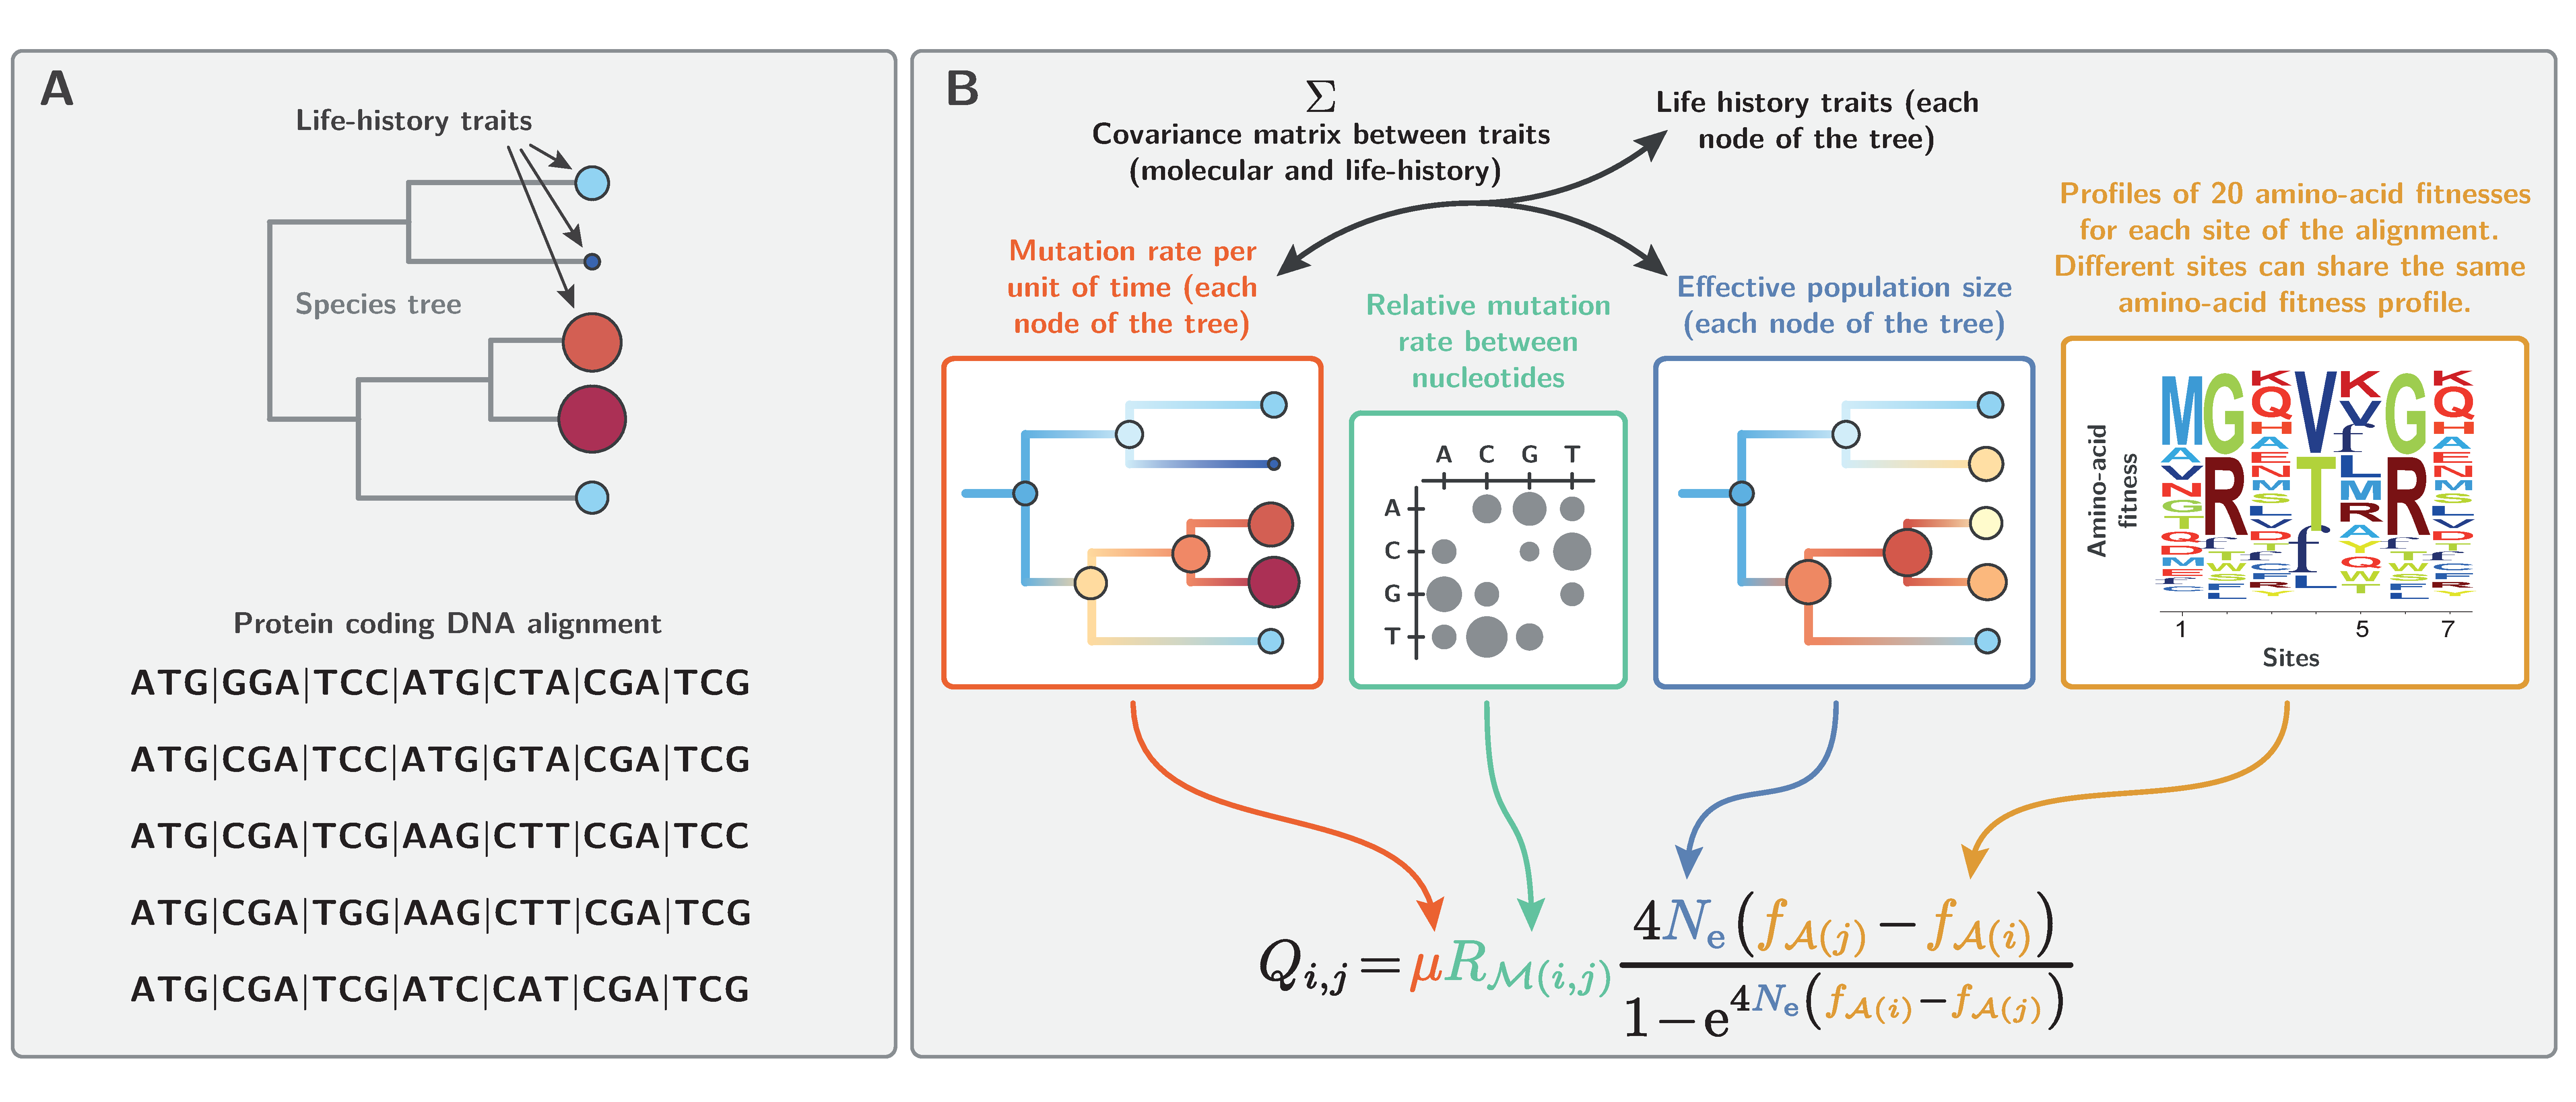
\includegraphics[width=\textwidth] {model_summary.pdf}
    \caption[Model summary]{
    Model summary.
    Panel A.
    Our method requires a given rooted topology, and an alignment of protein-coding \acrshort{DNA} for the extant species.
    Optionally, the method can use quantitative life-history traits at the leaves of the tree, and dated estimation for the internal nodes of the tree.
    Panel B.
    Our Bayesian inference model estimates selection coefficients, mutation rate, intensity of genetic drift and the age of the internal nodes.
    Effective population since~($\Ne$) and mutation rate per unit of time~($\mu$) are considered fluctuating branch-wise, but assumed constant across all sites of the \acrshort{DNA} sequence.
    Conversely, the selection coefficient of amino acids are considered changing for sites along the \acrshort{DNA} sequence, but are considered constant across the tree.
    Branch heterogeneity is modelled as an auto-correlated log-Brownian process, meaning our model estimates correlation coefficients between quantitative traits (as input), $\Ne$, and $\mu$, where phylogenetic inertia is accounted for.
    Synonymous substitutions are leveraged to estimates branch-wise mutation rate~($\mu$).
    Site-specific rates of non-synonymous substitutions across the tree is leveraged to estimate site-wise selection coefficient~($\Fit$).
    Branch-specific rates of non-synonymous substitutions across the sequence is leveraged to estimate branch-wise genetic drift~($\Ne$).
    }
    \label{fig:modelSummary}
\end{figure}

Formally, DNA coding sequences are modelled at the level of the codon, where for each codon site (triplet of nucleotides), a change of codon means a change in \acrshort{DNA} but not necessarily in amino-acid.
The substitution rate (per unit of time) from codon $\ci$ to $\cj$, denoted $\submatrix_{\itoj}$, is equal to the total rate of mutation (per unit of time) at the level of the population~($2\Ne\mu_{\itoj}$) multiplied by the probability of fixation of the mutation:
\begin{equation}
{\submatrix_{\itoj}}
    = 2 \Ne \mu_{\itoj} p_{\mathrm{fix}}(\itoj)
\end{equation}
In the case of synonymous mutations, which we assumed are neutral, the probability of fixation is independent of the original and target codon, and equal $1/2 \Ne$.
Finally, ${\submatrix_{\itoj}}$ simplifies to:
\begin{equation}
    \submatrix_{\itoj} = \mu_{\itoj}
\end{equation}
The mutation rate $\mu_{\itoj}$ depends on the underlying nucleotide change between the codons $\ci$ and $\cj$.
First, if codon $\ci$ to $\cj$ are not neighbours, $\mu_{\itoj}$ is equal to $0$.
Second, if codon $\ci$ and $\cj$ are only one mutation away, $\mu_{\itoj}$ is given by the nucleotide relative rate~(${\mutmatrix_{\nucitoj}}$) scaled by the mutation rate per time~($\mu$).
Technically, the $4$-dimensional nucleotide relative rate matrix~($\Mutmatrix$) is normalized such that we expect $1$ substitution per unit of time, hence the scaling by $\mu$.

In the case of non-synonymous mutations, the probability of fixation depends on the difference in fitness~\citep{Ohta1992} between the amino-acid encoded by the initial and final codons:
\begin{equation}
    \label{eq:mutationSelection}
    {\submatrix_{\itoj}} = \mu_{\itoj} \dfrac{4 \Ne \left({\fitj - \fiti}\right)}{{1 - \e^{4 \Ne \left({\fiti - \fitj}\right)} }}
\end{equation}
where $\Fit$ is a $20$-dimensional vector specifying the log-fitness for each amino-acid, and $\aai$ is the amino-acid encoded by codon $i$.
We see from this equation that, $\fit$ and $\Ne$ are confounded, such that increasing the effective population size while decreasing the fitnesses by the same factor leads to the same substitution rate.

In the model presented in this manuscript, $\Ne$ and $\mu$ are allowed to vary between species (across branches) as a multivariate log-Brownian process, but assumed constant along the \acrshort{DNA} sequence.
In a multivariate log-Brownian process, traits are modelled together as a vector-valued time-dependent random process, parameterized by a covariance matrix between traits~($\Covariancematrix$).
Altogether, values of the multivariate process at each node of the tree, a covariance matrix and divergence times are jointly estimated.
Once the traits are sampled at all nodes, traits along each branch is taken as the average between extremities of this branch.
Technically, the precision matrix (invert of covariance matrix) is distributed as an invert Wishart, meaning the prior matrix is diagonal, pushing the correlation coefficients between traits toward $0$.
The work presented here implemented the branch heterogeneity in a Bayesian context, as in \textit{CoEvol}~\citep{Lartillot2011}.
Conversely, amino-acid fitness profiles $\Fit$ are assumed to vary across sites, but are considered constant along the tree.
The work presented here relies on the Bayesian nonparametric random-effect approach, developed to estimate site-heterogeneous amino-acid fitnesses as in \textit{PhyloBayes}~\citep{Rodrigue2010}.
Our Bayesian implementation, written in C++ in the software \textit{BayesCode}, is publicly available at \url{https://github.com/ThibaultLatrille/bayescode}.

The phylogenetic codon model presented here makes several additional assumptions on the evolutionary processes generating the observed alignment.
First, the species tree topology is supposed to be known, and each gene should match the species tree, meaning genes are strict orthologs (no paralogs and no horizontal transfers).
Second, there is no epistasis (interaction between sites), such that any position of the sequence has its own independent evolutionary process and a substitution at one position does not affect the substitution process at other positions.
Third, from a population genetic perspective, we assumed sites of the protein to be unlinked, or equivalently the mutation rate is low enough such that there is no Hill-Robertson interference nor genetic hitchhiking.
Fourth, we assume \acrshort{DNA} sequences to be representative of the species, not taking into account the sampling effect tending to over-represent weakly deleterious mutations present at low frequencies.


\section{Results}
\label{sec:Results}

\begin{figure}[htbp]
    \centering
    \begin{minipage}{0.32\linewidth}
        \includegraphics[width=\linewidth, page=1]{simulations/BranchWise_SimuDiv_SiteMutSelBranchNe_BranchCorrelation_Log10BranchLength}
    \end{minipage}
    \llap{\raisebox{-1.1cm}{\scriptsize A\hspace{0.35cm}}}\hfill
    \begin{minipage}{0.32\linewidth}
        \includegraphics[width=\linewidth, page=1]{simulations/SimuPoly_SiteMutSelBranchNe_BranchCorrelation_Log10BranchLength}
    \end{minipage}
    \llap{\raisebox{-1.1cm}{\scriptsize B\hspace{0.35cm}}}\hfill
    \begin{minipage}{0.32\linewidth}
        \includegraphics[width=\linewidth, page=1]{simulations/SimuFold_SiteMutSelBranchNe_BranchCorrelation_Log10BranchLength}
    \end{minipage}
    \llap{\raisebox{-1.1cm}{\scriptsize C\hspace{0.35cm}}}\hfill
    \begin{minipage}{0.32\linewidth}
        \includegraphics[width=\linewidth, page=1]{simulations/BranchWise_SimuDiv_SiteMutSelBranchNe_BranchCorrelation_LogPopulationSize}
    \end{minipage}
    \llap{\raisebox{-1.1cm}{\scriptsize D\hspace{0.35cm}}}\hfill
    \begin{minipage}{0.32\linewidth}
        \includegraphics[width=\linewidth, page=1]{simulations/SimuPoly_SiteMutSelBranchNe_BranchCorrelation_LogPopulationSize}
    \end{minipage}
    \llap{\raisebox{-1.1cm}{\scriptsize E\hspace{0.35cm}}}\hfill
    \begin{minipage}{0.32\linewidth}
        \includegraphics[width=\linewidth, page=1]{simulations/SimuFold_SiteMutSelBranchNe_BranchCorrelation_LogPopulationSize}
    \end{minipage}
    \llap{\raisebox{-1.1cm}{\scriptsize F\hspace{0.35cm}}}\hfill
    \caption[Inferred and simulated branch length and $\Ne$]{
    Inferred values in vertical axis against simulated value in horizontal axis.
    In the top row (panels A, B and C), branch length in expected number of substitutions for each branch of the tree.
    In the bottom row (panels D, E and F), $\Ne$ for each node (including leaves) of the tree, relative to $\Ne$ at the root of the tree.
    In the left panels (A and D), simulation under the mutation-selection approximation, as to test the soundness of the inference framework.
    In middle panels (B and E), simulation accounting for small population size effects~($5000$ individuals at the root), site linkage and short term fluctuation of $\Ne$.
    In the right panels (C and F), simulation accounting for site epistasis in context of selection for protein stability, with fluctuation of the selection coefficient along the phylogeny.
    The tree root is $150$ million years old, where the initial population start with a mutation rate of $\smash{1e^{-8}}$ per site per generation, and generation time of $10$ years.
    These experiments confirm that signal in the placental mammalian tree can allow to reliably infer the direction of change in $\Ne$, even if linkage disequilibrium, short term fluctuation of $\Ne$ and finite population size effects are not accounted for in the inference framework.
    However, the presence of epistasis between sites is a serious threat to the inference of $\Ne$.
    }
    \label{fig:simulations}
\end{figure}

\subsection{Simulated experiments}
\label{sec:ResultsSimulated}
The inference framework was first tested using independently simulated alignments (see Methods).
With the aim of applying the inference method to empirical dataset in placental mammals, the simulation parameters were chosen to match the empirical regime of total branch length (expected number of substitutions) from root to leaves.

A first series of simulations was meant to test the soundness of our inference framework, by simulating essentially under the model used for inference, although with an independently developed software.
The mutation-selection approximation was assumed to be valid, and sites were simulated under different fitness profiles.
In addition, $\Ne$ varies at the tree nodes but otherwise remains constant along each branch.
In this context, simulated branch length and $\Ne$ could be recovered appropriately by our inference method, as depicted in figure~\ref{fig:simulations}, panel A \& D.
Unfortunately, assumptions made for this simulations are almost certainly violated in practice.
First, $\Ne$ should change continuously along a branch, between each generation of the population.
Second, having a separate process for each site is equivalent to have no linkage between sites (free recombination), an assumption that should be relaxed.
Third, the probability of fixation (equation~\ref{eq:mutationSelection}) does not hold in small finite population.

For these reasons, we performed a second more challenging series of simulations.
The finite population was modelled explicitly in a Wright-Fisher simulator, tracking the frequency of each allele at each generation along the phylogeny.
Such simulator accounts for small population size effects, hitchhiking of weakly deleterious mutations during selective sweep and background selection due to linkage disequilibrium.
Fluctuations of $\Ne$ and mutation rate were also fluctuating continuously along the branch of the tree.
Moreover, noise was added by accounting for short-term fluctuations of $\Ne$ on the order of $20\%$ per generation.
The simulated branch length and $\Ne$ could be robustly recovered by the inference framework in this context, as depicted in figure~\ref{fig:simulations}, panel B \& E.

However, if the results are encouraging to apply the method on empirical data, we rely on the assumption of site-independent fitness landscape, which is almost certainly broken in practice.
Finally, we implemented a more complex, site-dependent fitness landscape accounting for the $3$-dimensional structure of protein and interaction between sites.
In such a model, the conformational stability of the protein determines the probability of being in the folded state, a proxy for fitness~\citep{Williams2006, Goldstein2011, Pollock2012}.
During a simulation, at a particular codon site, the fitness landscape is dependent on the actual amino acids present in the vicinity of this particular site (see section~\ref{subsec:protein-folding-probability} in supplementary materials).
Our inference framework could recover the simulated branch length (figure~\ref{fig:simulations}, panel C), but hardly retrieves the simulated $\Ne$ in the context of site-dependent epistasis (figure~\ref{fig:simulations}, panel F).
This effect can, however, be explained by the predicted independence of $\dnds$ to changes in $\Ne$ in this specific model of protein stability~\citep{Goldstein2013}.
Such independence between $\dnds$ and $\Ne$ is due to the structure of the fitness landscape, where a decrease in $\Ne$ leads to a sequence further to the optimal protein where the curvature of the fitness landscape is steeper, resulting in a higher selection coefficient exactly compensating the decrease in $\Ne$, and the scaled selection coefficient is (almost) constant.
Additionally, under a Fisher geometric landscape developed in supplementary materials (section~\ref{subsec:fisher-geometric-landscape}) and also incorporating epistasis, branch length is reliably estimated while $\Ne$ is also more difficult to estimate.

\subsection{Empirical experiments}
\label{sec:ResultsEmpirical}
\begin{figure}[htbp]
    \centering
    \begin{minipage}{0.411\linewidth}
        \includegraphics[valign=t, width=\linewidth, page=1, clip, trim=0cm 0cm 15.35cm 0.15cm]{mammals/18CDS_SiteMutSelBranchNe_R1_LogPopulationSize}
    \end{minipage}
    \begin{minipage}{0.158\linewidth}
        \includegraphics[valign=t, width=\linewidth, page=1, clip, trim=0cm -2.2cm 0cm 0cm]{mammals_species}
    \end{minipage}
    \begin{minipage}{0.411\linewidth}
        \reflectbox{\includegraphics[valign=t, width=\linewidth, page=1, clip, trim=0cm 4.48cm 15.35cm 0cm]{mammals/18CDS_SiteMutSelBranchNe_R1_LogMutationRatePerTime}}
        \includegraphics[valign=b,width=\linewidth, page=1, clip, trim=0cm 0cm 15.35cm 32.3cm]{mammals/18CDS_SiteMutSelBranchNe_R1_LogMutationRatePerTime}
    \end{minipage}
    \caption[Example of inferred $\Ne$ and $\mu$ on placental mammals dataset]{
    Example of inferred $\Ne$ and $\mu$ on placental mammals dataset.
    Inferences were performed on a randomly chosen set of $18$ coding sequences (CDS) out of $226$ highly conserved CDS~($<1\%$ of gaps).
    Only highly conserved CDS were retained such that the assumption of constant fitness landscape is not incautiously broken by protein with changing function and/or adaptive selection.
    Brownian processes along the tree are represented for effective population size~($\Ne$, left panel) and mutation rate per site per unit of time~($\mu$, right panel).
    Mean values of \acrshort{MCMC} (after burn-in) are obtained at each node of the tree, hence a gradient can be extrapolated along each branch.
    At each node, the inner circle represents the lower bound of the \acrshort{MCMC} $90\%$ confidence interval, and the outer circle represent the upper bound, as to give visual input into the range of estimation.
    $\mu$ spanned almost $2$ order of magnitude, and if we assume the root to be $105$My old~\citep{Kumar2017}, the rescaled mutation rate per site per year in extant species is between $\smash{1.1e^{-10}}$ and $\smash{7.8e^{-9}}$.
    $\Ne$ at the root of the tree is arbitrarily set to $1$, and all values are relative to the root.
    }
    \label{fig:mammals_popsize_and_mutrate}
\end{figure}

We reconstructed long-term changes of effective population size~($\Ne$) and mutation rate per site per unit of time~($\mu$) in placental mammals, with alignments extracted from OrthoMam database~\citep{Ranwez2007,Scornavacca2019}.
Life-history traits (LHT) for longevity, age at maturity and weight were obtained from AnAge database~\citep{DEMAGALHAES2009,Tacutu2012}.
We focused our analysis on 77 taxa for which information is available for at least one LHT.

In the result of this analysis, depicted in figure~\ref{fig:mammals_popsize_and_mutrate}), we visually observe a global trend of increased $\Ne$ throughout the tree around $90$ and $60$ My.
We also observe $\Ne$ to be lower in \textit{Cetacea} and \textit{Camelidae}, while being higher in \textit{Rodentia} and \textit{Pecora}.
In some clades we can see a decrease along a single branch of the tree, for example \textit{Heterocephalus glaber} or \textit{Acinonyx jubatus}.

The analysis of the covariance matrix presented in table~\ref{fig:mammals_correlation}, discarding phylogenetic inertia, shows that $\Ne$ is positively correlated~($r^2 = 0.44$) with the mutation rate per unit of time, which is compatible with the assumption that large population are small-sized and with a shorter generation time.
Moreover the effective population size is negatively correlated with longevity, age at maturity and weight (Table~\ref{fig:mammals_correlation}), consistent with the observation that larger population have small-sized and short-lived individuals~\citep{Galtier2016,Romiguier2014}.
The partial-correlation coefficients (see definition section~\ref{subsec:partial-correlation-coefficient} and table~\ref{tab:table-partcor-mammals} in supplementary materials) are not significantly different from $0$.

However, if the trend of $\Ne$ would be in the right direction, the magnitude of inferred $\Ne$ is vastly underestimated by our method, with a ratio of $2.5$ between the maximum and minimum $\Ne$ in extant species (see figure~\ref{fig:mammals_popsize_and_mutrate}).
To assess the reproducibility of our inference, we analysed a concatenated random sample of $18$ highly conserved coding sequences~($\leq 1\%$ of gaps in the alignment), and repeated the procedure on different random samples of $18$ CDS.
Overall the estimation of $\Ne$ is reproducible for a random subset of CDS, as depicted in figure~\ref{fig:mammals_repeatability}.

We performed other empirical experiments using a group of isopod species that have made multiple independent transitions to subterranean environments.
Protein coding DNA sequences alignment and qualitative life-history traits such as habitat (surface or underground), pigmentation (depigmented, partially depigmented or pigmented) and ocular structure (anophthalmia, microphthalmia, or ocular) are available for these species~\citep{Saclier2018}.
Estimation of $\Ne$ reveals a correlation between qualitative life-history traits and $\Ne$, presented section~\ref{sec:empirical-data-in-isopods} in supplementary materials.
However, these correlations are sensitive to phylogenetic inertia since multivariate log-Brownian does not accommodate qualitative traits, although this particular dataset is composed of surface and subterranean species reducing biases.
Finally, our empirical framework was also applied in drosophila and related to genome size  (see~\ref{sec:empirical-data-in-primates} and~\ref{sec:empirical-data-in-drosophila} in supplementary materials).

\begin{table}[htbp]
    \centering
\noindent\adjustbox{max width=\textwidth}{%
\begin{tabu}{|c||c|c|c|c|c|}
\hline
\textbf{Correlation ($\bm{\rho}$)} & $\bm{N_{\mathrm{e}}}$ & $\bm{\mu}$ & \textbf{Maximum longevity } & \textbf{Adult weight } & \textbf{Female maturity }\\
\hhline{|=#=|=|=|=|=|}
$\bm{N_{\mathrm{e}}}$ & - & $0.439^{**}$ & $-0.523^{**}$ & $-0.544^{**}$ & $-0.47^{**}$\\\hline
$\bm{\mu}$ & - & - & $-0.832^{**}$ & $-0.835^{**}$ & $-0.833^{**}$\\\hline
\textbf{Maximum longevity } & - & - & - & $0.827^{**}$ & $0.845^{**}$\\\hline
\textbf{Adult weight } & - & - & - & - & $0.809^{**}$\\\hline
\textbf{Female maturity } & - & - & - & - & -\\\hline
\end{tabu}}

    \caption[Traits correlation]{
    Correlation coefficient between effective population size~($\Ne$), mutation rate per site per unit of time~($\mu$), and life-history traits (Maximum longevity, adult weight and female maturity), taking account phylogenetic inertia.
    Correlation coefficients are between $-1$ and $1$.
    Asterisks indicate strength of support of the posterior probability to be different than $0$ (pp) as $\smash{^{*}} pp > 0.95$ and $\smash{^{**}} pp > 0.975$.
    Observed correlations are compatible with the interpretation that large populations are composed of small, short-lived individuals.
    Moreover if the mutation rate per generation is considered constant in first approximation, the mutation rate per unit of time is positively correlated to generation rate, hence to population size.
    }
    \label{fig:mammals_correlation}
\end{table}


\section{Discussion}
\label{sec:Discussion}
% Summary 
Mechanistic phylogenetic codon models explicitly define the substitution rates as function of the mutation rate, selection and genetic drift.
Applied on an alignment of \acrshort{DNA} coding sequence, the mechanistic model can estimate amino-acid fitness landscapes along the \acrshort{DNA} sequence.
On the other hand, molecular comparative framework reconstruct the joint evolution of life history, molecular and population-genetics traits along the phylogeny, intrinsically including phylogenetic inertia.
Combined together, the resulting framework can reconstruct site-heterogeneous amino-acid fitness landscapes, estimates the age of internal nodes, and finally reconstitute branch-heterogeneous life-history traits, mutation rate ($\mu$) and effective population size ($\Ne$), with their correlation.
Testing the method against simulated alignments suggests the signal is strong enough in protein-coding \acrshort{DNA} alignment to infer selection at the site level, and long-term changes in $\Ne$ and $\mu$ using a phylogenetic approach.
In placental mammals, $\Ne$ correlates negatively with longevity, weight and maturity, and positively with $\mu$.
Our observations suggest that the empirical signal is strong enough such that we can infer the directional trends in changes.

% Longvariance in Ne 
If the trend of variations in $\Ne$ is in right direction, the magnitude of change across the phylogeny with a ratio of $2.5$ is greatly inferior to the expected variation observed in mammals~\citep{Galtier2016}.
Different mechanisms not accounted for by the model could explain such a low variation of reconstructed $\Ne$.

First, genetic hitchhiking, Hill-Robertson interference, and short-term fluctuations of $\Ne$ could generate this effect.
However, inference made on alignments simulated by Wright-Fisher model accounting for linkage tends to show that this effect is not strong enough in the regimes explored.

Second, $\mu$ and $\Ne$ could also be fluctuating along the genome.
This assumption needs to be tested, though we expect that relaxing this assumption would not change drastically the magnitude of inferred $\Ne$ since some of this fluctuation is absorbed by site-specific fitness profiles.

Third, the \acrshort{DNA} sequences could also be misaligned in some sites.
However we observe the same magnitude of inferred $\Ne$ for different set of genes indicating this might not be the primary reason.

Fourth, the genes selected in our alignments could be under adaptive evolution, or their function could have changed.
More precisely, the fitness profile at each site could change with time, either due to Red-Queen dynamics or due to epistasis because amino-acid substitutions occurred at other sites.
Simulation of \acrshort{DNA} coding sequences under an epistatic landscape seemingly points to epistasis being the principal factor to be investigated, since $\Ne$ could not be appropriately estimated in such a case.
Independently, the magnitude of inferred $\Ne$ is quite similar for the placental mammals dataset and the primates dataset, while we would expect a greater discrepancy at longer phylogenetic scale.
An explanation could be that epistasis is more prevalent at longer time-scale, because the total number of substitutions from root to leaves is greater, hence the fitness landscape is less stable.
Thought modelling epistasis in an inference framework is a complex biological, mathematical and computational problem, this work points to a potential signal of epistasis that could be retrieved in phylogenetic context.
% None equilibrium properties

% Perspective : codon bias
Our model also assumes no bias in codon usage, though the strength of selection for a particular codon (or set of codons) among all synonymous possible codons has been proved to be substantial~\citep{Yang2008,Plotkin2011}.
This assumption can be relaxed by implementing codon preferences that are shared across all sites such that $41$ more parameters would be required in total.
Such implementation would provide the advantage of estimating codon usage biases, and of accounting for its confounding effect while estimating selection and $\Ne$.

% Perspective: 
Bayesian computations shown in this study are based on relatively small alignments ($20,000$ sites at most), and with a limited parametrization in the number of fitness profile categories~($50$).
Analysing execution duration of the program (not shown) leads to conclude that the number of fitness profile categories is the limiting step to expand the computation.
To estimate a more statistically stable genome-wide $\Ne$, we could develop an extended version leveraging parallel computing, where each coding sequence has its own computing process and own profile categories, but the $\Ne$ would be shared by all computing processes.
By increasing the number of categories per gene, the magnitude of inferred $\Ne$ would also increase, since fitness profiles would be sharper.

% Perspective: increase power
Mutation-selection models originated with the aim of increasing the power to detect adaptive evolution, by modelling explicitly the confounding effect of purifying selection.
However, by assuming constant $\Ne$ along a phylogeny, the statistical power to detect sites under adaptive evolution is not optimal.
Fitness profiles estimated are averaged along the phylogeny and are more seemingly neutral than our estimated profiles under our present framework (see section~\ref{subsec:fitness-profile-entropy} and table~\ref{tab:table-entropy-aa-mutselne} in supplementary materials).
Even though our method requires more computing resources to estimate fitness profiles, it provides a better null model of purifying selection to test against the presence of adaptive evolution.

% Comparison with other methods
Other methods have recently been developed to reconstruct phylogenetic changes in $\Ne$.
For example, a method recently developed by \citet{Brevet2019} uses \acrshort{DNA} coding sequences, a distribution of fitness effects, polymorphism and generation time for some present-day species to reconstruct $\Ne$ along the phylogeny~\citep{Brevet2019}.
This method also based on the quasi-neutral theory of evolution allows to estimate the absolute value of $\Ne$, even for species where the polymorphism is unavailable.
Here our method requires neither generation time nor polymorphism, and the fitness effects are not constrained to a specific distribution.
However, the inferred values are solely relative and the computation requires more computing resources.

% Perspective: Short and long-term Ne
Estimating $\Ne$ in a mutation-selection phylogenetic model relies on the relation between $\Ne$ and relative strength of drift, where ultimately the signal of drift comes from the relative rate of substitutions.
However, they do not leverage a second aspect of $\Ne$ at the population level, which determines the neutral genetic diversity that can be maintained~($\pi=4\Ne \mu \tau$, where $\tau$ is the generation time).
Hence, polymorphic data give us independent empirical estimates of $\Ne$, based on the assumption that mutations are neutral.
In principle, our mechanistic model could be extended to leverage polymorphism within species in the case of differential selection, a method which has been previously pioneered in the case of $3$ species and using a distribution of fitness effect~\citep{Wilson2011}.
More generally, the nearly-neutral theory of evolution defines a long-term $\Ne$, which might be different from the short-term definition of $\Ne$~\citep{Platt2018}.
Thus we could ask if empirical independent estimations of $\Ne$ from within species (polymorphic diversity) and between species (substitutions) are congruent, and if not what are the mechanisms responsible for this discrepancy.

% Relation to ecology
Notwithstanding theoretical considerations on the quasi-neutral theory of evolution, empirical clues about the long-term trends in the direction of genetic drift, and changes between species allows to open a large diversity of ecological and evolutionary questions.
Spatial and temporal changes of genetic drift along ecological niches and events can be investigated to disentangle the underlying evolutionary and ecological pressures.

\begin{figure}[htbp]
    \centering
    \begin{minipage}{0.32\linewidth}
        \includegraphics[width=\linewidth, page=1]{mammals/18CDS_SiteMutSelBranchNe_Rep_Log10BranchLength-1-2}
    \end{minipage}
    \llap{\raisebox{-1.1cm}{\scriptsize A\hspace{0.35cm}}}\hfill
    \begin{minipage}{0.32\linewidth}
        \includegraphics[width=\linewidth, page=1]{mammals/18CDS_SiteMutSelBranchNe_Rep_Log10BranchLength-1-3}
    \end{minipage}
    \llap{\raisebox{-1.1cm}{\scriptsize B\hspace{0.35cm}}}\hfill
    \begin{minipage}{0.32\linewidth}
        \includegraphics[width=\linewidth, page=1]{mammals/18CDS_SiteMutSelBranchNe_Rep_Log10BranchLength-1-4}
    \end{minipage}
    \llap{\raisebox{-1.1cm}{\scriptsize C\hspace{0.35cm}}}\hfill
    \begin{minipage}{0.32\linewidth}
        \includegraphics[width=\linewidth, page=1]{mammals/18CDS_SiteMutSelBranchNe_Rep_LogPopulationSize-1-2}
    \end{minipage}
    \llap{\raisebox{-1.1cm}{\scriptsize D\hspace{0.35cm}}}\hfill
    \begin{minipage}{0.32\linewidth}
        \includegraphics[width=\linewidth, page=1]{mammals/18CDS_SiteMutSelBranchNe_Rep_LogPopulationSize-1-3}
    \end{minipage}
    \llap{\raisebox{-1.1cm}{\scriptsize E\hspace{0.35cm}}}\hfill
    \begin{minipage}{0.32\linewidth}
        \includegraphics[width=\linewidth, page=1]{mammals/18CDS_SiteMutSelBranchNe_Rep_LogPopulationSize-1-4}
    \end{minipage}
    \llap{\raisebox{-1.1cm}{\scriptsize F\hspace{0.35cm}}}\hfill
    \caption[Repeatability of experiments]{
    Repeatability of experiments.
    $3$ independent inferences were performed on a randomly chosen set of $18$ coding sequences (CDS) out of $226$.
    Each plot is a correlation between a pair of experiments for a given parameter.
    Mutation rate per unit of time~($\mu$), is represented in the top row (panels A, B and C), while effective population size~($\Ne$) is represented in the bottom row (panels D, E and F).
    For each node of the tree, the mean posterior of the parameter~($\Ne$ or $\mu$) over the \acrshort{MCMC} (after burn-in) is represented in blue dots, green solid lines are the $90\%$ confidence interval of the \acrshort{MCMC}.
    Solid red line is the regression line between experiments.
    Inference of $\mu$ is more reproducible than $\Ne$, but overall the experiment is reproducible for a random subset of CDS.
    }
    \label{fig:mammals_repeatability}
\end{figure}


\section{Materials and Methods}
\label{sec:MatMet}
The parameterization of the models is described as a Bayesian hierarchical model, containing the prior distributions and parameters of the model.
This hierarchical model is formally represented as directed acyclic graph, depicted in figure~\ref{fig:DAG-MutSelNe}.

\subsection{Nucleotide mutation rates}
The generalized time-reversible nucleotide mutation rate matrix $\Mutmatrix$ is a function of the nucleotide frequencies $\Mutequi$ and the relative rate $\Exchan$.
$\Mutequi = (\mutequi_A , \mutequi_C , \mutequi_G , \mutequi_T)$ is the equilibrium base frequency vector, giving the frequency at which each base occurs at each site.
$\Exchan = \left( \exchan_{AC}, \exchan_{AG}, \exchan_{AT}, \exchan_{CG}, \exchan_{CT}, \exchan_{GT}\right)$ is the vector of exchangeabilities between nucleotides.
Altogether, the rate matrix is:
\begin{equation}
    \label{eq:gtr-mutrates}
    \Mutmatrix =
    \begin{pmatrix}
        - & {\exchan_{AC}\mutequi_C} & {\exchan_{AG}\mutequi_G} & {\exchan_{AT}\mutequi_T} \\
        {\exchan_{AC}\mutequi_A} &                        - & {\exchan_{CG}\mutequi_G} & {\exchan_{CT}\mutequi_T} \\
        {\exchan_{AG}\mutequi_A} & {\exchan_{CG}\mutequi_C} &                        - & {\exchan_{GT}\mutequi_T} \\
        {\exchan_{AT}\mutequi_A} & {\exchan_{CT}\mutequi_C} & {\exchan_{GT}\mutequi_G} & -
    \end{pmatrix}
\end{equation}
By definition, the sum of the entries in each row of the nucleotide rate matrix $\Mutmatrix$ is equal to $0$, giving the diagonal entries:
\begin{equation}
    \mutmatrix_{a,a} = - \sum\limits_{ b \neq a} \mutmatrix_{a,b}
\end{equation}
The prior on the exchangeabilities $\Exchan$ is a uniform Dirichlet distribution of dimension $6$:
\begin{equation}
    \label{eq:DistribExchan}
    \Exchan \sim \mathrm{Dir}\left( \dfrac{1}{6} , 6\right).
\end{equation}
The prior on the equilibrium base frequencies $\Mutequi$ is a uniform Dirichlet distribution of dimension $4$:
\begin{equation}
    \label{eq:DistribMutequi}
    \Mutequi \sim \mathrm{Dir}\left( \dfrac{1}{4} , 4\right)
\end{equation}
The general time-reversible nucleotide matrix is normalized such that the total flow equals to $1$:
\begin{equation}
    \sum\limits_{a \in \{A, C, G, T\}} - \mutequi_a \mutmatrix_{a,a} = 1.
\end{equation}

\subsection{Site-dependent selection}
\label{sec:profiles}
For each category $\Setcat$, a $20$-dimensional fitness profile $\Base\catexp$ (summing to $1$) is distributed as a Dirichlet of center $\Basecenter$ and concentration $\baseconc$:
\begin{equation}
    \label{eq:DistribBase}
    \Base\catexp \sim \mathrm{Dir}\left( \Basecenter,\ \baseconc \right),\ \Setcat.
\end{equation}
For an alignment of size $\Nsite$, each site $\Setsite$ is assigned a fitness profile category of amino acids $\catsite \in \catInterval $.
The total number of sites falling in each fitness profile category $\cat$ is denoted $\catmultivar_{\cat}$.
The $\Ncat$-dimensional vector $\catMultiVar$ is distributed as a multinomial of event probabilities $\StickBreaking$:
\begin{align}
    \label{eq:DistribMultinomial}
    \catMultiVar \sim \mathrm{Multinomial}\left( \StickBreaking \right).
\end{align}
The event probabilities $\Ncat$-dimensional vector~($\StickBreaking$) of falling into each category is distributed as a stick-breaking Dirichlet process:
\begin{align}
    \label{eq:DistribStickBreaking}
    \begin{split}
        & \StickBreaking \sim \mathrm{StickBreaking}\left( \Ncat, \stickbreakinghyper \right)\\
        \iff & \stickbreaking_{\cat} = \stick_{\cat}\cdot \prod _{{\indice=1}}^{{\cat-1}}\left(1-\stick_{\indice}\right),\ \Setcat,
    \end{split}
\end{align}
where $\stick_{\cat}$ are i.i.d.
from a beta distribution
\begin{equation}
    \label{eq:Beta}
    \stick_{\cat} \sim \mathrm{Beta}\left( 1, \stickbreakinghyper \right),\ \Setcat.
\end{equation}
The Malthusian fitness selection coefficients $\Fit\siteexp$ at site $\site$, are obtained by taking the logarithm of the fitness profile assigned to this site:
\begin{equation}
    \label{eq:sitefitness}
    \Fit\siteexp = \log \left( \Base^{\left( \catsite \right)} \right),\ \Setsite.
\end{equation}

\subsection{Dated tree}
The topology of the rooted phylogenetic tree is supposed to be known and is not estimated by the model.
The model estimates the dates at which branches split, thus the dated tree requires $\Ntaxa - 2$ internal node ages that are free parameters, where $\Ntaxa$ is the number of extant taxa (leaves of the tree).
The node ages $\age\nodeexp,\ \Setinternal$ are drawn uniformly such that a node cannot be younger than the oldest of its $2$ descendant children, and must also be younger than its parent:
\begin{equation}
    \label{eq:Distribage}
    \age\nodeexp \ \sim \mathcal{U}\left( \mathrm{max}\left(\age^{(\mathrm{children})} \right), \age^{(\mathrm{parent})} \right)
\end{equation}
By definition, leaf ages are all set to $0$. The root age is set arbitrarily to $1$, but if fossils data are also available the dated tree can be rescaled into absolute time using cross-multiplication.\\
The duration of the branch~($\branchtime\branchexp$), for each branch $\Setbranch$ is defined as the difference in ages between the oldest node at the tip of the branch $\age^{(\nodeUp)}$, and the youngest node $\age^{(\nodeDown)}$:
\begin{equation}
    \label{eq:ageTobranchtime}
    \branchtime\branchexp = \age^{(\nodeUp)} - \age^{(\nodeDown)}.
\end{equation}

\subsection{Branch dependent traits}
The effective population size $\Ne$ and mutation rate per unit of time $\mu$ are assumed to evolve along the phylogeny, and to be correlated.
If quantitative life-history-traits (LHT) are also available for some nodes of the tree (leaves and/or internal nodes), they are also assumed to evolve along the phylogeny and to be correlated between them, and with $\Ne$ and $\mu$.
The total number of traits (counting $\Ne$, $\mu$ and all user-defined LHT) is denoted $\Ntrait$.
Their fluctuations are modelled by a $\Ntrait$-dimensional log-Brownian process $\Brownian\nodeexp$ at each node $\Setnode$ of the tree, including the root and leaves.
The first dimension (indexed by $0$) of the log-Brownian contain $\Ne$, and the second dimension (indexed by $1$) contains $\mu$.
The log-Brownian process and variables of interest~($\mu$ and $\Ne$) are linked by an exponential transformation:
\begin{equation}
    \begin{dcases}
        \Ne\nodeexp = \e^{ \brownian_{0}\nodeexp } \\
        \mu\nodeexp = \e^{ \brownian_{1}\nodeexp },
    \end{dcases}
\end{equation}
where the effective population size at the root is set to $1$ for identifiability of the fitness profiles.
It is important to note that inferred correlation between $\Ne$, $\mu$ and other LHT is thus in the log space, and that quantitative LHT must be inputted in log scale.

Along a branch $\Setbranch$ of the tree, a log-Brownian process starts at the oldest node at the tip of the branch~($\nodeUp$), and ends at the youngest node~($\nodeDown$).
However we are interested in the average over the branch to define the codon substitution matrices along the branch.
In the case of log-Brownian process, the most likely path (or geodesic) from $\Brownian^{(\nodeUp)}$ to $\Brownian^{(\nodeDown)}$ is the straight line, and therefore, it would make sense to take the mean value of $\e^{\Brownian\nodeexp}$ along this geodesic.
We then have $\Ne\branchexp$ and $\mu\branchexp$ for each branch $\Setbranch$ of the tree:
\begin{equation}
    \label{eq:branchNemu}
    \begin{dcases}
        \Ne\branchexp = \dfrac{\e^{\brownian_{0}^{(\nodeDown)}} - \e^{\brownian_{0}^{(\nodeUp)}}}{\brownian_{0}^{(\nodeDown)} - \brownian_{0}^{(\nodeUp)}} \\
        \mu\branchexp = \dfrac{\e^{\brownian_{1}^{(\nodeDown)}} - \e^{\brownian_{1}^{(\nodeUp)}}}{\brownian_{1}^{(\nodeDown)} - \brownian_{1}^{(\nodeUp)}}.
    \end{dcases}
\end{equation}

Moreover, the rate of change of the log-Brownian process per unit of time is constant and determined by the positive semi-definite and symmetric covariance matrix $\CovarianceMatrix$, and thus the distribution of $\Brownian^{(\nodeDown)}$ is multivariate Gaussian, with mean $\Brownian^{(\nodeUp)}$ and variance $\branchtime\branchexp \CovarianceMatrix$:
\begin{equation}
    \label{eq:DistribBrownian}
    \Brownian^{(\nodeDown)} \sim \mathcal{N}\left(\Brownian^{(\nodeUp)}, \branchtime\branchexp \CovarianceMatrix \right),\ \Setbranch
\end{equation}

\begin{figure}[H]
    \centering
    \begin{tikzpicture}[->,>=stealth',shorten >=1pt,auto,node distance=0.6cm and 1.2cm,semithick]
        \tikzstyle{every state}=[]

        \node[state] (P) {$\Probmatrix\branchsiteexp$};
        \node[state] (Q) [below right=of P] {$\Submatrix\branchsiteexp$};
        \node[state] (R) [below right=of Q] {$\Mutmatrix$};
        \node[state] (BL) [above right=of P] {$\branchlength\branchexp$};
        \node[state] (Ne) [above right=of Q] {$\Ne\branchexp$};
        \node[state] (Bb) [above right=of Ne] {$\Brownian\nodeexp $};
        \node[state] (Mu) [left=of Bb] {$\mu\branchexp$};
        \node[state] (f) [right=of Q] {$\Fit\siteexp $};
        \node[state] (Ex) [BLUE, below right=of R] {$\Exchan$};
        \node[state] (Equi) [BLUE, right=of R] {$\Mutequi$};
        \node[state] (dT) [above left=of Bb] {$\branchtime\branchexp $};
        \node[state] (T) [BLUE, right=of dT] {$\age\nodeexp$};
        \node[state] (Base) [BLUE, above right=of f] {$\Base\catexp$};
        \node[state] (cat) [BLUE, right=of f] {$\catsite$};
        \node[state] (ExH) [RED, right=of Ex] {$\dfrac{1}{6}, 6$};
        \node[state] (EquiH) [RED, right=of Equi] {$\dfrac{1}{4}, 4$};
        \node[state] (Unif) [RED, right=of T] {$\uniform$};
        \node[state] (C) [BLUE, right=of Bb] {$\contrast\branchexp$};
        \node[state] (Cov) [BLUE, right=of C] {$\Covariancematrix$};
        \node[state] (baseH) [RED, right=of Base] {$\baseconc, \Basecenter $};
        \node[state] (sb) [BLUE, right=of cat] {$\StickBreaking$};
        \node[state] (CovH) [RED, right=of Cov] {$\covariancekappa, \covariancedf$};
        \node[state] (sbH) [RED, right=of sb] {$\stickbreakinghyper$};

        \path
        (Q) edge [black] node [above right] {\ref{eq:Probmatrix}} (P)
        (dT) edge [black] node [above left] {\ref{eq:branchlength}} (BL)
        (Mu) edge [black] node [] {} (BL)
        (BL) edge [black] node [] {} (P)
        (Ne) edge [black] node {} (Q)
        (R) edge [black] node {} (Q)
        (Bb) edge [black] node {} (Ne)
        (Bb) edge [black] node [below] {\ref{eq:branchNemu}} (Mu)
        (f) edge [black] node [above] {\ref{eq:subrates}} (Q)
        (Ex) edge [black] node [] {} (R)
        (Equi) edge [black] node [below] {\ref{eq:gtr-mutrates}} (R)
        (T) edge [black] node [above] {\ref{eq:ageTobranchtime}} (dT)
        (dT) edge [black] node {} (Bb)
        (Base) edge [black] node {} (f)
        (cat) edge [black] node [above] {\ref{eq:sitefitness}} (f)
        (ExH) edge [dashed, BLUE] node [above] {\ref{eq:DistribExchan}} (Ex)
        (EquiH) edge [dashed, BLUE] node [above] {\ref{eq:DistribMutequi}} (Equi)
        (Unif) edge [dashed, BLUE] node [above] {\ref{eq:Distribage}} (T)
        (C) edge [black] node [above] {\ref{eq:independent_contrast}} (Bb)
        (Cov) edge [dashed, BLUE] node [above] {\ref{eq:Distribcontrast}} (C)
        (baseH) edge [dashed, BLUE] node [above] {\ref{eq:DistribBase}} (Base)
        (sb) edge [dashed, BLUE] node [above] {\ref{eq:DistribMultinomial}} (cat)
        (CovH) edge [dashed, BLUE] node [above] {\ref{eq:Distribcovariance}} (Cov)
        (sbH) edge [dashed, BLUE] node [above] {\ref{eq:DistribStickBreaking},\ref{eq:Beta}} (sb);
    \end{tikzpicture}

    \caption[Directed acyclic graph of dependencies between variables]{
    Directed acyclic graph (DAG) of dependencies between variables.
    Nodes of the directed acyclic graph are the variables, and edges are the functions.
    Hyper-parameters are depicted in {\color{RED}{red}} circles, random variables in {\color{BLUE}{blue}} circles, and transformed variables in black.
    {\color{BLUE}{Blue}} dashed line denotes a drawing from a random distribution, and black solid lines denote a function.
    For a given node, all the nodes pointing toward him (upstream) are its dependencies which determines its distribution.
    The other way around, following the arrows in the DAG (downstream), simple prior distributions are combined together to form more complex joint prior distribution which ultimately defines the prior distribution of the model.
    }\label{fig:DAG-MutSelNe}
\end{figure}

We make a change of variable as to define the branch-wise independent contrast $\contrast\branchexp$:
\begin{align}
    \contrast\branchexp &= \dfrac{\brownian^{(\nodeDown)} - \brownian^{(\nodeUp)}}{\sqrt{\branchtime\branchexp}} \\
    \label{eq:independent_contrast}
    \iff \brownian^{(\nodeDown)} &= \brownian^{(\nodeUp)} + \sqrt{\branchtime\branchexp}\contrast\branchexp
\end{align}
And these contrasts are i.i.d.
from a multivariate normal distribution:
\begin{equation}
    \label{eq:Distribcontrast}
    \contrast\branchexp \sim \mathcal{N}\left(\bm{0}, \Covariancematrix \right), \Setbranch
\end{equation}
The prior on the covariance matrix is an invert Wishart distribution, parameterized by $\covariancekappa=1$ and with $\covariancedf=\Ntrait + 1$ degrees of freedom:
\begin{equation}
    \label{eq:Distribcovariance}
    \CovarianceMatrix \sim \mathrm{Wishart}^{-1} (\covariancekappa \Identitymatrix, \covariancedf)
\end{equation}

\subsection{Codon {substitution} rates}
For a given branch $\branch$ and a given site $\site$, the codon substitution rate (per unit of time) matrix $\Submatrix\branchsiteexp$ is given by:
\begin{equation}
    \label{eq:subrates}
    \begin{dcases}
        \submatrix\branchsiteexp_{\itoj} = 0\text{ if $\ci$ and $\cj$ are not neighbors,} \\
        \submatrix\branchsiteexp_{\itoj} = \mutmatrix_{\nucitoj}\text{ if $\ci$ and $\cj$ are synonymous,} \\
        \submatrix\branchsiteexp_{\itoj} = \mutmatrix_{\nucitoj} \dfrac{4\Ne\branchexp \left({\fitj\siteexp - \fiti\siteexp}\right)}{{1 - \e^{4\Ne\branchexp\left({\fiti\siteexp - \fitj\siteexp}\right)} }} \text{ if non-syn.,}\\
        \submatrix\branchsiteexp_{\ci, \ci} = - \sum\limits_{ \cj \neq \ci, \jSetCodon} \submatrix\branchsiteexp_{\itoj},
    \end{dcases}
\end{equation}
The branch lengths $\branchlength\branchexp$ are defined as the expected number of neutral substitutions per \acrshort{DNA} site along a branch:
\begin{equation}
    \label{eq:branchlength}
    \branchlength\branchexp = \mu\branchexp \branchtime\branchexp
\end{equation}
Together, the probability of {transition} between codons for a given branch $\branch$ and site $\site$ is:
\begin{equation}
    \label{eq:Probmatrix}
    \Probmatrix\branchsiteexp = \e^{\branchlength\branchexp \Submatrix\branchsiteexp},
\end{equation}
which are the matrices necessary to compute the likelihood of the data ($\data$) given the parameters of the model using the pruning algorithm.

\subsection{Bayesian implementation}
\label{sec:Bayesian}
Monte Carlo Markov chains (\acrshort{MCMC}) are run for 4000 points and the first 1000 points are discarded as burn-in, the convergence is then assessed (see section~\ref{subsec:chain-convergence} in supplementary materials), as both site-specific fitness and branch $\Ne$ have the same posterior mean.
Most phylogenetic MCMC samplers target the distribution over the model parameters, which means that they have to repeatedly invoke the pruning algorithm to recalculate the pruning-based likelihood which is most often the limiting step of the \acrshort{MCMC}.
An alternative, which is used here, is to do the \acrshort{MCMC} conditionally on the detailed substitution history $\subhistory$, thus doing the \acrshort{MCMC} over the augmented configuration~($\subhistory$, $\data$), under the target distribution obtained by combining the mapping-based likelihood with the prior over model parameters.

The key idea that makes this strategy efficient is that the mapping-based likelihood depends on compact summary statistics of $\subhistory$, leading to very fast evaluation of the likelihood.
On the other hand, this requires to implement more complex \acrshort{MCMC} procedures that have to alternate between:
\begin{enumerate}
    \item sampling $\subhistory$ conditionally on the data and the current parameter configuration.
    \item re-sampling the parameters conditionally on $\subhistory$.
\end{enumerate}

To implement the mapping-based \acrshort{MCMC} sampling strategy, we first sample the detailed substitution history $\subhistory$ for all sites along the tree.
Several methods exist for doing this~\citep{Nielsen2002,Rodrigue2008}.
Then, we write down the probability of $\subhistory$ given the parameters, and finally, we collect all factors that depend on some parameter of interest and make some simplifications.
This ultimately leads to relatively compact sufficient statistics (see section~\ref{sec:sufficient-statistics-mutselne} in supplementary materials) that are fast to evaluate~\citep{Irvahn2014,Davydov2016}.

As an example, making an \acrshort{MCMC} move on the $\Ne$ at a given node of the tree is drastically faster since only the mapping-based likelihood (using path sufficient statistics) at the neighbouring branches of the node is necessary, and not computing the likelihood for the all trees.

\subsection{Correlation between traits}
\label{sec:Correlation}
The correlation between trait $\traiti$ and trait $\traitj \in \traitInterval$ can be obtained from the covariance matrix $\Covariancematrix$:
\begin{equation}
    \rho_{\traiti, \traitj} = \dfrac{\Covariancematrix_{\traiti, \traitj}}{\sqrt{\Covariancematrix_{\traiti, \traiti} \Covariancematrix_{\traitj, \traitj}}}
\end{equation}

\subsection{Simulations}
\label{sec:Simulation}
To test the robustness of the model, $4$ parameterized simulators were developed: \textit{SimuDiv}, \textit{SimuPoly}, \textit{SimuFold} \& \textit{SimuGeo}.
All $4$ simulators use a log-Brownian multivariate process to model conjointly the changes in the mutation rate per generation, the generation time and $\Ne$, in logarithm space.
\textit{SimuDiv}, \textit{SimuFold} \& \textit{SimuGeo} all simulate point substitutions along the phylogenetic tree.
The simulator starts from an initial sequence at equilibrium.
The change in fitness is computed for all possible mutant, hence computing all strictly positive substitution rates.
At each point, the next substitution is chosen proportional to the rate as in Gillespie algorithm.
At each node, the process is split, and finally the process is stopped at the leaves of the tree.
\textit{SimuPoly} simulates explicitly each generation along the phylogeny under a Wright-Fisher population, consisting of three steps: mutation, selection and genetic drift of alleles.
Mutations are drawn randomly based on the probability of mutation.
Drift is modelled as a multinomial distribution on the allele counts.
We assumed that the \acrshort{DNA} sequence is composed of exons, with no linkage between exons, and total linkage of sites within an exon.
Moreover, in \textit{SimuPoly} $\Ne$ can also be modelled as a sum of a log-Brownian process and an Ornstein-Uhlenbeck process.
The log-Brownian motion takes into account long-term fluctuations, while the Ornstein-Uhlenbeck can take into account short fluctuations of $\Ne$.
In \textit{SimuDiv} and \textit{SimuPoly} each codon site contribute independently to the fitness depending on the encoded amino acids, through site-specific amino-acid fitness profiles experimentally determined~\citep{Bloom2017}.
However, in \textit{SimuFold} the fitness of a sequence is computed as the probability of the protein to be in the folded state.
\textit{SimuFold} is in practice a C++ adaptation of a Java code previously published~\citep{Goldstein2016, Goldstein2017}, where we allow for changes in $\Ne$ and $\mu$ along a phylogenetic tree.
Section~\ref{sec:supp-mat-simulations} in supplementary materials describes the models in more details, as well as performance of the inference model against them.
The simulators written in C++ are publicly available under MIT license at \url{https://github.com/ThibaultLatrille/SimuEvol}


\thispagestyle{empty}
\chapter[Substitution rate susceptibility]{Substitution rate response to changes in effective population size and protein expression level.}
{\hypersetup{linkcolor=GREYDARK}\minitoc}
\label{chap:GenoPhenoFit}
\section{Introduction}

Molecular sequences differ across species due to the particular history of nucleotide substitutions along their respective lineages.
These substitutions in turn are the result of the interplay between evolutionary forces such as mutation and selection, whose relative forces are determined by the amount of random genetic drift.
These forces have effects at different levels: mutations are carried by molecular sequences, selection is mediated at the level of individuals, while random genetic drift is a population sampling effect.
Yet, they jointly contribute to the long-term molecular evolutionary process.
Thus, the challenge of molecular evolution is to tease out their respective contributions, based on comparative analyses.

One main aspect of this challenge is to correctly evaluate the role of random drift in the long term evolutionary process.
Population genetics theory implies that the strength of drift, due to the stochastic sampling of mutations, is less pronounced in lineage with large effective population size ($\Ne$), and as a consequence, the purification by selection of weakly deleterious mutations is more effective.
This fundamental idea is at the core of the nearly-neutral theory of evolution.
This theory posits that a substantial fraction of mutations are deleterious or weakly deleterious, and as result predicts that the substitution rate (relative to the neutral expectation), called $\omega$, decreases along lineages with higher $\Ne$~\citep{Ohta1972, Ohta1992}.

This prediction has been more quantitatively examined under the assumption that the selective effects of mutations are drawn from a fixed distribution of fitness effects (\acrshort{DFE})~\citep{Kimura1979, Welch2008}.
Assuming a gamma \acrshort{DFE}, a key result obtained in this context is an approximate allometric scaling of $\omega$ as a function of $\Ne$ (i.e. $\omega \sim \Ne^{-k}$), where $k$ is the shape parameter of the \acrshort{DFE}.
In practice, DFEs are strongly leptokurtic, which thus predicts a weak negative relation between $\omega$ and $\Ne$.

The quantity $\omega$ is an observable of the molecular evolutionary process, at least if we can separately estimate the rate of neutral and selected substitutions in a phylogenetic or comparative context.
Practically, in the case of protein-coding \acrshort{DNA} sequences, and assuming that synonymous mutations are neutral, while non-synonymous changes affecting the amino-acid sequence are under selection, $\omega$ can be identified with the ratio of non-synonymous over synonymous substitution rates , called $\dnds$.
Thus the nearly-neutral argument translates into a predicted decrease in $\dnds$ as a function of long-term changes in $\Ne$.

The context of protein-coding sequences fostered another modelling approach, based on genotype-fitness maps instead of distribution of fitness effects.
In this alternative approach, the selective effect of a mutation depends on the fitness of both the source and the target amino acids involved in the mutation event~\citep{Halpern1998, Rodrigue2010, Tamuri2012}.
More fundamentally, the fitness depends solely on the current genotype, not on the trajectory of mutations leading to this sequence.
For example, if the target amino acid has a higher fitness than the current amino acid, the selective effect of the mutation is positive, and reciprocally negative for a lower fitness.
Such a modelling approach predicts higher substitution rates between amino acid with similar biochemical properties.
Even though this modelling approach differs substantially from the one assuming a fixed \acrshort{DFE}, it also predicts a negative correlation between $\omega$ and $\Ne$, at least when the process is at equilibrium~\citep{Spielman2015, DosReis2015}.

Conversely, one striking theoretical result was the proof that $\omega$ is in fact predicted to be independent of $\Ne$ under relatively very general circumstances, namely, whenever (i) the fitness is a log-concave function of a phenotype and (ii) the phenotype itself is equimutable.
Equimutability states that the distribution of phenotypic changes due to mutations is independent the current phenotype of individuals~\citep{Cherry1998}.
This general theoretical argument has been invoked in the context of \textit{in silico} experiments of protein sequence evolution, assuming that proteins are under selection for their thermodynamic stability, with fitness being proportional to folding probability of the protein~\citep{Goldstein2013}.
Thermodynamic stability is itself computed using a 3D structural model of the protein.
These computational experiments have led to the observation that $\omega$ is essentially independent of $\Ne$.
An explanation proposed for this result is that the distribution of changes in free energy of folding ($\EmpiricalDeltaDeltaG$) due to mutations is approximately independent of the current free energy ($\DeltaG$), thus making the free energy of folding essentially equimutable.

However, the equimutability assumption is a relatively strong one, which also conflicts with combinatorial considerations about the relation between sequence and phenotype~\citep{Serohijos2012}.
For example, if a protein sequence is already maximally stable, only destabilizing (or neutral) mutations can occur.
More generally, assuming that the stability of a protein sequence reflects an underlying fraction of positions having already accepted destabilizing amino acids, then the probability of destabilizing mutational events is in turn expected to directly depend on the current stability of the protein.

Altogether, depending on the theoretical model mapping sequence to fitness, $\omega$ can be either independent or negatively correlated to $\Ne$, or even positively if considering adaptive evolution and environmental changes~\citep{Lanfear2014}.

Empirically, variation in $\omega$ between lineages has been inferred using phylogenetic codon models applied to empirical sequences~\citep{Yang1998,Zhang2004}.
Confronting branch-specific $\omega$ estimates to life-history traits such as body mass or generation time uncovered a positive correlation~\citep{Popadin2007, Nikolaev2007}.
Subsequently, integrative inference methods combining molecular sequences and life-history traits have also found that $\omega$ correlates positively with traits such as longevity and body mass~\citep{Lartillot2011, Figuet2017}.
Since lineage with a large body size and extended longevity typically correspond to species with low $\Ne$~\citep{Romiguier2014}, these empirical correlations suggest a negative correlation between $\omega$ and $\Ne$, thus confirming the theoretical prediction of the nearly-neutral theory of evolution.
However, the universality and robustness of the correlation between $\omega$ and life-history traits is still debated.
Results have not been entirely consistent across independent studies, the correlation was found to be either not statistically significant~\citep{Lartillot2012}, or even in the opposite direction depending on the specific clade under study or the potential biases taken into account~\citep{Lanfear2010, Nabholz2013, Lanfear2014, Figuet2016}.

If empirical evidence for a negative correlation of $\omega$ with $\Ne$ is still not totally convincing, another empirical correlation is known to be much more robust.
Indeed, expression level or protein abundance is one of the best predictors of $\omega$, with highly expressed proteins typically having lower $\omega$ values, a correlation clearly significant although relatively weak~\citep{Duret2000, Rocha2004, Drummond2005a, Zhang2015, Song2017}.
Theoretical models, also based on protein stability, have been invoked to explain this negative correlation between $\omega$ and expression level~\citep{Wilke2006, Drummond2008}.
According to this argument, selection against protein misfolding due to toxicity, which is stronger for more abundant proteins, induces abundant proteins to evolve toward greater stability, resulting in a more constrained and more slowly evolving protein coding sequence~\citep{Serohijos2012}.

The possibility that expression level and $\Ne$ might play similar roles in the evolution of proteins has already been noticed.
More precisely, under models of selection against protein misfolding, the free energy of folding $\DeltaG$ is predicted to vary similarly along a gradient of either $\Ne$ or expression level~\citep{Serohijos2013}.
As a corollary, under strict equimutability of $\DeltaG$, these computational models imply that $\omega$ should also be independent of expression level~\citep{Serohijos2012}, thus like what is predicted with regards to changes in $\Ne$.

Altogether, both theoretical results and empirical analyses are not yet conclusive about the question of how $\omega$ depends on $\Ne$ and expression level.
In particular, the theoretical response of $\omega$ to changes in both $\Ne$ and expression level has not been quantified and, most importantly, has not been related to the specific map between genotype, phenotype and fitness.
Such an analytical development would be useful to more decisively confront the theoretical predictions relating $\omega$ to both $\Ne$ and expression level to empirical data.
Ultimately, relating proteins structural parameters to the response of $\omega$ would help to bridge the gap between protein thermodynamics on one side and comparative genomics on the other side.

Lastly, the theoretical results discussed so far are valid only at the mutation-selection-drift balance.
In a non-equilibrium regime, however, and at least under a model assuming a site-independent genotype-fitness map, an increase in $\Ne$ first leads to an increase in $\omega$ caused by adaptive substitutions, and subsequently a decrease in $\omega$ due to stronger purifying selection in the long term~\citep{Jones2016}.
Studying only equilibrium properties can thus be misleading.
For that reason, the dynamic response of $\omega$ to changes in $\Ne$ must also be addressed, quantified, and its connection with the underlying selective landscape better characterized.
Dynamic properties of $\omega$ to changes in $\Ne$ are of theoretical interest but are also empirically relevant, such that, if overlooked they could thwart the relation between theoretical expectations and empirical estimates.

In this context, the aim of the present study is to characterize the dynamic and equilibrium response of $\omega$ to changes in $\Ne$ and expression level, and to relate this response to structural parameters of the model.
To this effect, we develop a general mathematical approach to derive a quantitative approximation of the response of $\omega$ to changes in $\Ne$ and expression level, in the context of a given genotype-phenotype-fitness map, as depicted in figure~\ref{fig:Summary}.
In the light of previously published empirical estimates from protein thermodynamic and comparative genomics, we discuss the articulation between empirical data and our mechanistic model.
We also discuss some of the alternative biophysical mechanisms that could determine the selective landscape on protein-coding sequences, and how they would modulate the response of $\omega$ to changes in $\Ne$ and expression level.


\section{Results}

\subsection{Models of evolution}

The results that are presented below are valid for a general category of models of sequence evolution, based on an additive trait $x$, such that the coding positions of the sequence contribute additively to the trait.
The trait is under directional selection specified by a decreasing and log-concave fitness function $ \wrightfit (x)$.
As a specific example, we more specifically consider a model of protein evolution under the constraint of thermodynamic stability, as depicted in the left panel of figure~\ref{fig:Summary}.
This model is inspired from previous work~\citep{Williams2006, Goldstein2011, Pollock2012}, except that we make several simplifying assumptions, allowing us to derive analytical equations.

\begin{figure}[htbp]
    \centering
    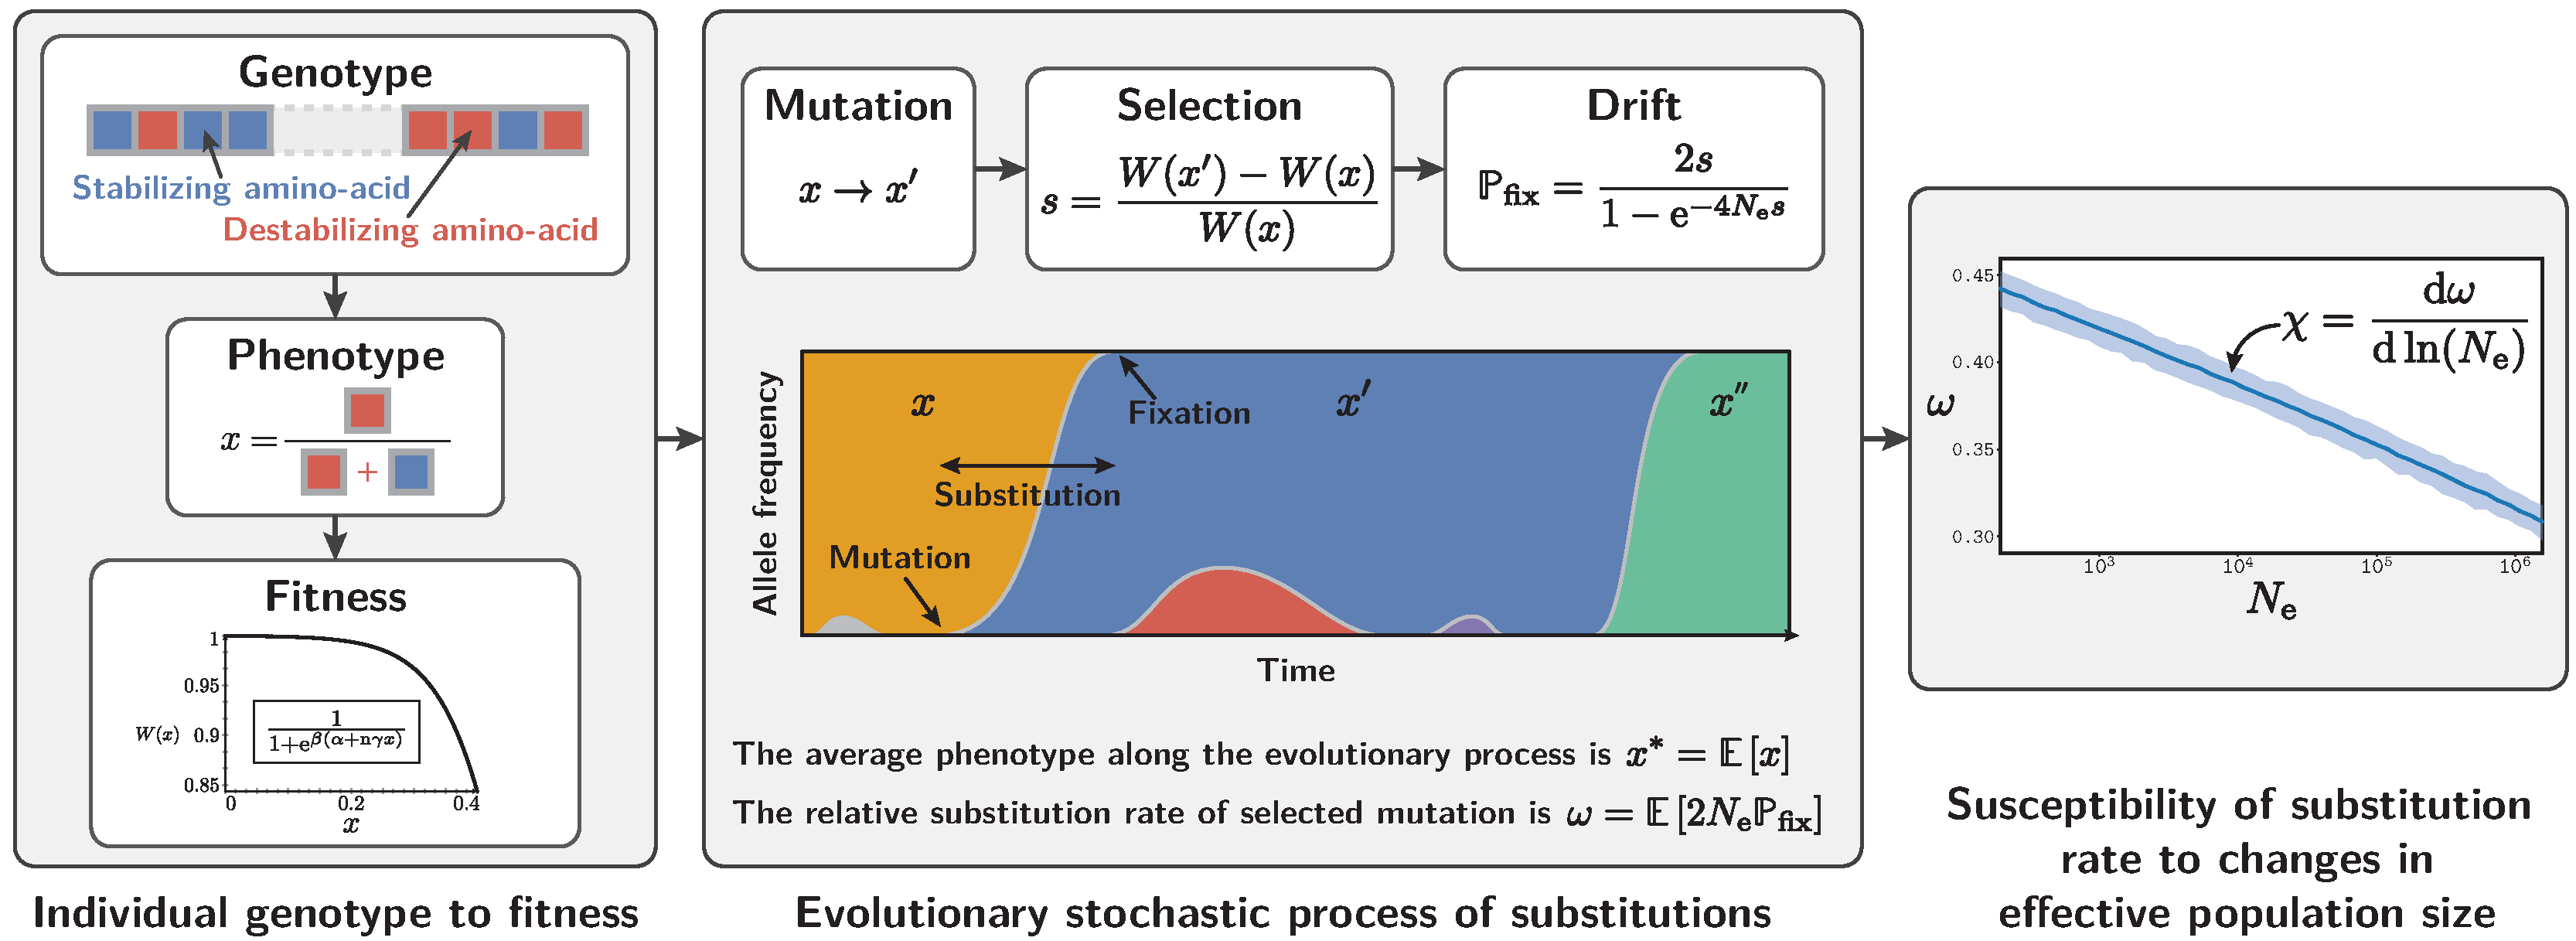
\includegraphics[width=\textwidth, page=1] {summary.pdf}
    \caption[Outline of the theoretical results]{
    Outline of the theoretical results.
    The genotype to fitness relationship is depicted in the left panel.
    The genotype is defined as the complete state of the amino-acid sequence.
    Subsequently, the phenotype ($x$) is a real-valued summary of the genotype, and is defined in our model as the fraction of destabilizing sites in the sequence.
    Finally, fitness is a decreasing log-concave function of the phenotype, depending on structural parameters of the model.
    Once defined the relation from genotype to fitness at the individual level, the evolutionary process is presented in the middle panel.
    The process consists of point substitutions of the amino-acid representative sequence of the population.
    Substitutions are mutation reaching fixation, thus the rate of substitution depends mechanistically on the interplay between mutation, selection and genetic drift.
    For a given effective population size $\Ne$, the evolutionary process result in an average value of the phenotype $\smash{x\eq}$ and also an average substitution rate (relative to the neutral rate) $\omega$.
    Averaging over time is equivalent to determining the statistical equilibrium, by ergodicity of the stochastic process, given we can derive the probabilities of transitions between phenotypes.
    The scaling of this equilibrium $\omega$ under a range of $\Ne$, presented in the right panel, gives us the slope of this relationship, called the susceptibility $\chi$, as a function of the structural parameters defined in the phenotype-fitness map.
    }
    \label{fig:Summary}
\end{figure}
In the original biophysical model, protein stability is determined by the difference in free energy between the folded and unfolded conformations, called $\DeltaG$ and measured in kcal/mol.
Technically, free energy is computed based on the 3D conformation of the protein and using statistical potentials.
As a result, the stabilizing or destabilizing effect of an amino acid at a particular site depends on amino acids present in the vicinity in 3D conformation, thus implementing what has been called specific epistasis~\citep{Dasmeh2018}.

Here, we approximate this model such that the (de-)stabilizing effect at a particular site, such as measured by the $\EmpiricalDeltaDeltaG$ of the mutation, does not depend on other neighbouring residues, thus disregarding specific epistasis~\citep{Dasmeh2014}.
Instead, each site contributes independently and additively to $\DeltaG$.
In addition, we assume that, for each site of the sequence, only one amino acid is stabilizing the protein.
All $19$ other amino acids are equally destabilizing.
Each site bearing a destabilizing amino acid contributes an excess of $\DeltaDeltaG > 0$ (in kcal/mol) to the total $\DeltaG$.
To note, $\DeltaDeltaG$ and $\EmpiricalDeltaDeltaG$ are equivalent, however $\DeltaDeltaG$ is preferred for mathematical readability, and $\EmpiricalDeltaDeltaG$ will refer to the empirical estimate.
The smallest achievable value of $\DeltaG$, obtained when all amino acids of the sequence are stabilizing, is noted $ \DeltaGmin < 0$.
Similarly, $\EmpiricalDeltaGmin$ will refer to the empirical estimate of $\DeltaGmin$.
In this model, the most succinct phenotype of a given genotype (i.e. sequence) is just the proportion of destabilizing amino acids in the sequence, defined as $0 \leq x \leq 1$.
Thus $\DeltaG$ is a linear function of $x$:
\begin{align}
    \DeltaG (x) = \DeltaGmin + \NbrSites \DeltaDeltaG x,
\end{align}
where $\NbrSites$ is the number of sites in the sequence.

For a given $\DeltaG$, thermodynamic equations allows one to derive the proportion of protein molecules that are in the native (folded) conformation in the cytoplasm.
This fraction is assumed to be a proxy for fitness, motivated in part by the fact that a protein must be folded to perform its function.
A slightly different model will be considered below, in order to take into account protein expression level (see section~\ref{sec:expression}).

Analytically, the fitness function is given by the Fermi Dirac distribution and is typically close to $1$, leading to a first-order approximation~\citep{Goldstein2011}:
\begin{gather}
    \wrightfit (x) = \dfrac{1}{1 + e^{\beta (\DeltaGmin + \NbrSites \DeltaDeltaG x)}},\\
    \Rightarrow \wrightfit (x) \simeq 1 - e^{\beta (\DeltaGmin + \NbrSites \DeltaDeltaG x)},\\
    \Rightarrow \logfit (x) = \ln ( \wrightfit (x) ) \simeq e^{\beta (\DeltaGmin + \NbrSites \DeltaDeltaG x)},
\end{gather}
where $\wrightfit$ is the Wrightian fitness for a given phenotype and $\logfit $ is the Malthusian fitness (or log-fitness).
Here, $\DeltaGmin$ and $\DeltaDeltaG$ are defined as above, and the parameter $\beta$ is $1.686$ mol/kcal at $25 \degree C$ (or $298.2 \degree K$).

Of note, even though the phenotypic effect of a mutation at a given site does not depend on the amino-acids that are present at other sites (i.e. the trait is additive), the fitness effect of a mutation still depends on other sites (i.e. the log-fitness is not additive).
As a result, the molecular evolutionary process is site-interdependent, a property referred to as non-specific epistasis~\citep{Dasmeh2018}.

\subsection{Response of \texorpdfstring{$\omega$}{ω} to changes in \texorpdfstring{$\Ne$}{Nₑ}. Analytical approximation}

For a given effective population size $\Ne$, the evolutionary process reaches an equilibrium (figure~\ref{fig:Summary}, middle panel).
This substitution rate at this equilibrium, normalized by the substitution rate of neutral of mutations to discard the influence of the underlying mutation rate, is denoted $\omega$.
This relative rate can also be interpreted as the mean fixation probability of mutations scaled by the fixation probability of neutral alleles $p = 1 / {2 \Ne}$, the mean being weighted by the probability of occurrence of mutations in the population.
As a result, an $\omega < 1$ indicates that mutations are negatively selected on average, and $\omega$ decreases with increasing strength of purifying selection.

In this section we present an analytical approximate solution for the response of $\omega$ after a change in $\Ne$ (in log space), as depicted in the right panel of figure~\ref{fig:Summary}.
We call this response the susceptibility of $\omega$ to changes in $\Ne$, and denote it as $\chi$:
\begin{align}
    \chi = \frac{ \der \omega}{\der \ln (\Ne)} \label{eq:chi}
\end{align}
Deriving $\chi$ is done in two steps.
First, we determine the mean phenotype at equilibrium, when evolutionary forces of mutation, selection and genetic drift compensate each other.
Subsequently, differential calculus is used to compute the response of the equilibrium phenotype to a change in $\Ne$, which allows us to ultimately derive an equation for $\chi$.
The main results of our derivation are given both in the general case of any (log-concave) phenotype-fitness map, and in the specific case of the biophysical model introduced above.
A more detailed derivation is available in the supplementary materials (section~\ref{sec:susceptibility-after-a-change-in-Ne}).

For a given genotype, mutations can have various effects: they can increase or decrease the proportion of destabilizing amino acids, or do nothing if the mutation is between two destabilizing amino acids.
To derive the probabilities of such events to occur, we also make the simplifying assumption that all transitions between amino acids are equiprobable.
Altogether, any mutation in the sequence can then have a phenotypic effect of $0$ or $\dx=1 /\NbrSites$, with probabilities of transitions equal to:
\begin{gather}
    \begin{cases}
        \dx &\text{ with probability } 1-x, \\
        0 &\text{ with probability } \frac{18 x }{19}, \\
        -\dx &\text{ with probability } \frac{x}{19}.\\
    \end{cases} \label{eq:proba}
\end{gather}
In the extreme case of an optimal phenotype ($x = 0$), only destabilizing mutations are proposed.
Moreover, the probability to propose a stabilizing mutation (effect $-\dx$), or a neutral mutation (effect $0$), is proportional to $x$.
Conversely, the probability to propose a destabilizing mutation is equal to $(1-x)$.
As a result, the mutation bias is proportional to $(1-x)/x$.
This mutation bias fundamentally reflects a combinatorial effect, due to the number of mutational opportunities available in either direction.

Second, we need to determine the strength of selection acting on mutations.
Destabilizing mutations are selected against with a negative selection coefficient which can be approximated by:
\begin{align}
    s & \simeq \frac{1}{\NbrSites}\frac{ \partial \logfit (x) }{\partial x} \label{eq:s} \\
    \Rightarrow s & \simeq - \beta \DeltaDeltaG e^{\beta (\DeltaGmin + \NbrSites \DeltaDeltaG x)}, \label{eq:s-unfolded}
\end{align}
where $ \logfit = \ln (\wrightfit)$ is the log-fitness (or malthusian fitness).
Conversely, stabilizing mutations will be under positive selection with opposite sign but same absolute value.
It is important to realize that the selective effect is dependent on $x$.
Furthermore, because the fitness function is log-concave, the absolute value of $s$ increases with $x$.

Based on these expressions for the mutational and selective pressures, one can then study the trajectory followed by the evolutionary process.
Starting from an optimal sequence, mostly destabilizing mutations will occur, some of which may reach fixation and accumulate until selection coefficients against new deleterious mutations is too strong, at which point the protein will reach a point of equilibrium called marginal stability~\citep{Taverna2002, Bloom2007}.
Most importantly, the probability of fixation of mutations is affected by genetic drift, and thus depends on the effective population size ($\Ne$).
At the equilibrium between mutation, selection and drift, the process fluctuates through the occurrence of advantageous and deleterious substitutions compensating each other.
This equilibrium can be determined by expressing the constraint that the selection coefficient of substitutions is expected to be null on average~\citep{Goldstein2013}.
Formally, and after simplification, the equilibrium phenotype denoted $x\eq$ is given in the general case by:
\begin{align}
    \ln \left( \frac{1 - x\eq}{x\eq} \right) + \ln (19) & \simeq - \frac{4\Ne}{\NbrSites} \frac{ \partial \logfit (x\eq) }{\partial {x\eq}} \\
    \Rightarrow \ln \left( \frac{1 - x\eq}{x\eq} \right) + \ln (19) & \simeq 4\Ne \beta \DeltaDeltaG e^{\beta (\DeltaGmin + \NbrSites \DeltaDeltaG x\eq)} \text{,} \label{eq:equilibrium}
\end{align}
in the more specific case of the biophysical model.
This equation essentially expresses the mutation-selection equilibrium: the left-hand side of the equation is the log of the mutation bias at $x$, while the right-hand side is simply $4 \Ne s$, the scaled selection coefficient.

This equation cannot be solved explicitly for $x\eq$, but a qualitative intuition on the consequences of change in $\Ne$ to the equilibrium phenotype $x\eq$ is given in figure~\ref{fig:NeChangeInfluence}.
Intuitively, an increase in $\Ne$ results in a more optimal phenotype, closer to $0$.
The mutation bias (left-hand side of equation~\ref{eq:equilibrium}) decreases with $x$ while the strength of selection (right-hand side of equation~\ref{eq:equilibrium}) increases with $x$, and the equilibrium phenotype is obtained at their intersection.
An increase in $\Ne$ leads to shifting the selective response upward, which then results in a leftward shift of the equilibrium phenotype (i.e. closer to $0$).
The leftward shift is smaller for selective strengths characterized by a steeper curve, resulting in qualitatively weaker susceptibility of the equilibrium phenotype to changes in $\Ne$

\begin{figure}[htbp]
    \centering
    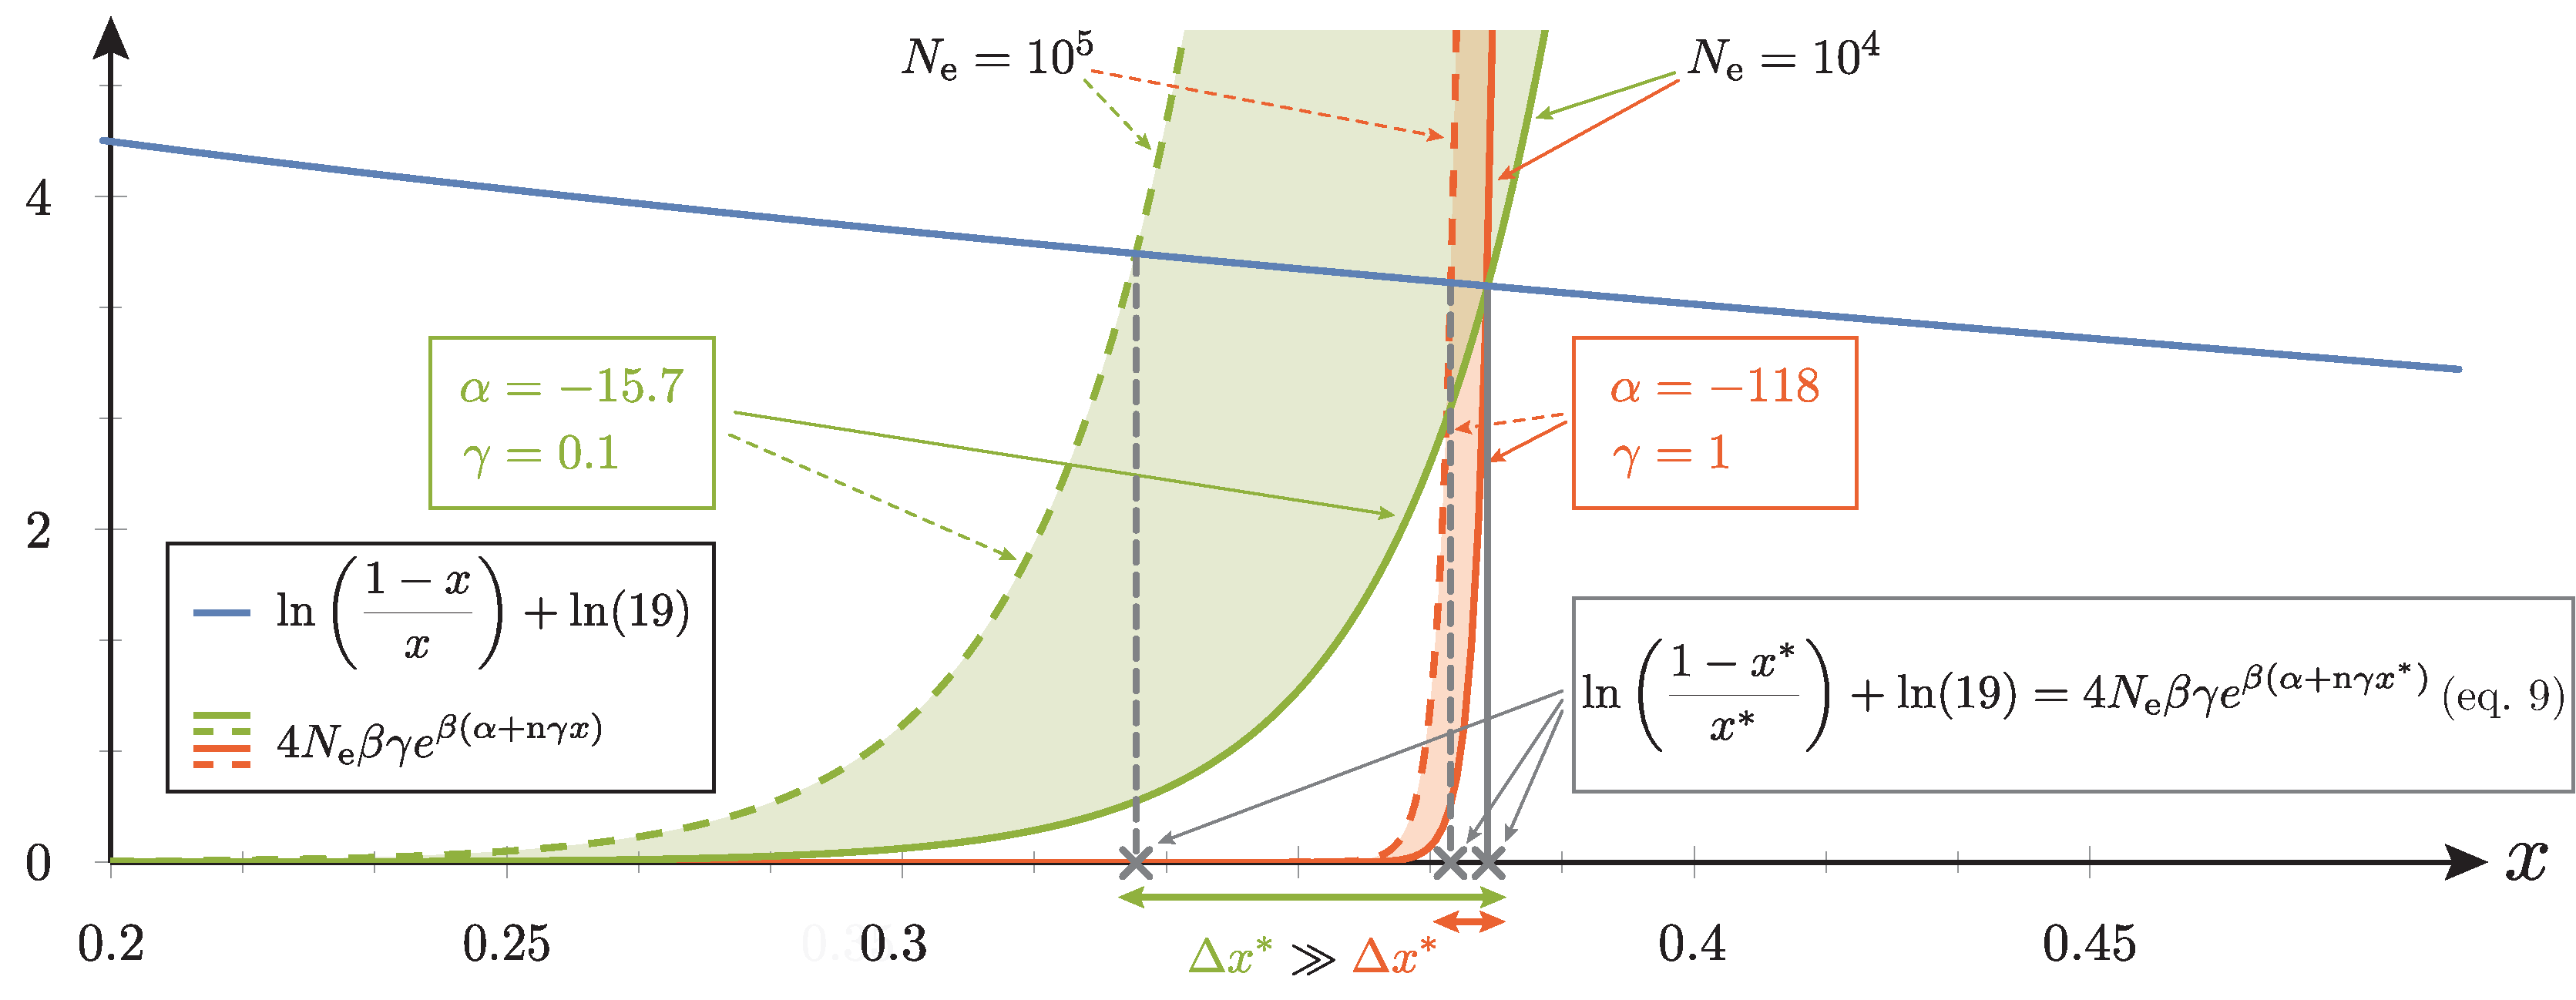
\includegraphics[width=\textwidth, page=1] {theoretical.pdf}

    \caption[Phenotype susceptibility after a change in $\Ne$]{
    Phenotype susceptibility after a change in $\Ne$.
    The equilibrium phenotype $x\eq$ is determined by the equation $\smash{\ln(\frac{1 - x\eq}{x\eq}) + \ln(19)=4\Ne \beta \DeltaDeltaG e^{\beta (\DeltaGmin + \NbrSites \DeltaDeltaG x\eq)}}$.
    The right-hand side of the equation increases exponentially with $x$ where $\NbrSites \DeltaDeltaG$ is the exponential growth rate ({\color{RED}red} and {\color{GREEN}green} curves).
    The parameter $\DeltaDeltaG$ is chosen such that $\DeltaDeltaG$ is increased by an order of magnitude in the red compared to the green curve, moreover, the value of $\DeltaGmin$ is chosen such that the equilibrium value $\smash{x\eq}$ is kept constant by solving numerically equation~\ref{eq:equilibrium}.
    Whenever $\NbrSites \DeltaDeltaG$ is large ({\color{RED}red solid} curve), the exponential growth is steep and increasing $\Ne$ (dotted curve) only changes subtly the equilibrium phenotype by a factor $\smash{\color{RED}\Delta x\eq}$.
    On the other hand, whenever $\NbrSites \DeltaDeltaG$ is low ({\color{GREEN}green} solid curve), the exponential growth is steadier and increasing $\Ne$ (dotted curve) involve a stronger susceptibility of the equilibrium phenotype by a factor $\smash{\color{GREEN}\Delta x\eq}$.
    Moreover, changes in $\smash{x\eq}$ reflects the changes in $\omega$ since both are approximately equal (equation~\ref{eq:dnds}).
    }
    \label{fig:NeChangeInfluence}
\end{figure}

The results obtained thus far only relate the equilibrium phenotype ($x\eq$) to $\Ne$.
To capture how $\omega$ varies with $\Ne$, we also need to obtain an expression for $\omega$ as a function of $x\eq$.
At equilibrium we can derive (section~\ref{subsec:mean-scaled-fixation-probability-omega-at-equilibrium} in supplementary materials) the expected substitution rate of mutations, and thus $\omega$, which simply approximates to:
\begin{gather}
    \omega \simeq x\eq \label{eq:dnds}
\end{gather}
This simple approximation is due to the fact that the substitutions between two destabilizing amino acids (which are neutral) compose the largest proportion of proposed mutations having a substantial probability of fixation (equation~\ref{eq:proba}).
In contrast, stabilizing mutations are rare, while destabilizing mutations have a low probability of fixation.
Since there is a fraction $x\eq$ of sites already occupied by a destabilizing amino-acid, these neutral substitutions occur at rate $x\eq$.

Combined together, these analytical approximations yield the susceptibility (equation~\ref{eq:chi}) of $\omega$ to a change in $\Ne$:
\begin{gather}
    \chi = \frac{ \der \omega}{\der \ln (\Ne)} \simeq - \frac{\frac{ \partial \logfit (x\eq) }{\partial {x\eq}}}{\frac{\NbrSites}{4 \Ne} \frac{\partial \ln [ (1 - x\eq) / x\eq ]}{\partial x\eq } + \frac{ \partial^2 \logfit (x\eq) }{\partial {x\eq}^2}}.
\end{gather}
The two terms of the denominator correspond to the derivative of respectively the mutational bias and the scaled selection coefficient, respectively.
However, the mutational bias decreases weakly with $x$ (blue curve on figure~\ref{fig:NeChangeInfluence}) while the strength of selection increases sharply with $x$ (red and green curves).
As a consequence, the derivative of the mutational bias is much lower than the derivative of the selection coefficient around the equilibrium point (i.e. the phenotype is \textit{nearly} equimutable).
The second term can therefore be ignored, which leads to a very compact equation for susceptibility $\chi$ in the general case:
\begin{gather}
    \chi \simeq - \frac{\frac{ \partial \logfit (x\eq) }{\partial {x\eq}}}{\frac{ \partial^2 \logfit (x\eq) }{\partial {x\eq}^2}}
\end{gather}
The susceptibility is thus equal to the inverse of the relative curvature, i.e. the ratio of the second to the first derivatives, of the log-fitness function, taken at the equilibrium phenotype.
Of note, this susceptibility is strictly negative for decreasing log-concave fitness functions, asserting that $\omega$ is a decreasing function of $\Ne$.
In addition, the susceptibility itself is low in absolute value (i.e. $\omega$ responds more weakly) for strongly concave log-fitness functions.
This equation quantitatively captures the intuition developed in figure~\ref{fig:NeChangeInfluence}, namely that the response of $\omega$ is very weak if the selection curve is very steep around the equilibrium set point (red curve compared to green curve).

In the specific case of the biophysical model, the susceptibility ($\chi$) further simplifies to:
\begin{gather}
    \chi \simeq -\dfrac{1}{\beta \NbrSites \DeltaDeltaG}, \label{eq:chi_application}
\end{gather}
meaning that $\omega$ is linearly decreasing with $\Ne$ (in log scale) since $\chi$ is independent of $x\eq$, or, in other words, that the exact value of the equilibrium phenotype has no impact on the slope.
Moreover, only the compound parameter $\beta \DeltaDeltaG \NbrSites$ has an impact on the slope of the linear relationship.
Thus, in particular, the slope of the linear relationship between $\omega$ and $\Ne$ is affected by $\DeltaDeltaG$ but not by $\DeltaGmin$.
Of note, empirically, only relative values of $\Ne$ (up to a multiplicative constant) are required to obtain an estimate of $\chi$.
% Although the general equation seems to suggest in appearance that elasticity only depends on the fitness function, in fact, what the biophysical model shows is that the elasticity can actually be modulated in two ways: by playing on the genotype / phenotype relationship (here, $\DeltaDeltaG$), or by playing on the fitness phenotype relationship (here, beta). All the more reason to consider beta as a potentially free parameter too.

\subsection{Response of \texorpdfstring{$\omega$}{ω} to changes in protein expression level}
\label{sec:expression}

Effective population size is not the sole predictor of $\omega$, and expression level (or protein abundance) is also negatively correlated to $\omega$.
However, our previous model, which assumes that fitness is proportional to the folded fraction, and is thus independent of protein abundance, does not express the fact that selection is typically stronger for proteins characterized by higher levels of expression.
An alternative biophysical model is to assume that each misfolded protein molecule has the same relative effect on fitness, caused by its toxicity for the cell~\citep{Drummond2005a, Wilke2006, Drummond2008, Serohijos2012}.

Ou general derivation can be directly applied to this case.
For a given protein with expression level $y$ and a cost $c$ representing the selective cost per misfolded molecule (positive constant), the fitness and selection coefficient can be defined as follows:
\begin{gather}
    \logfit (x) \simeq - c y e^{\beta (\DeltaGmin + \NbrSites \DeltaDeltaG x)} \\
    \Rightarrow s \simeq - \beta \DeltaDeltaG c y e^{\beta(\DeltaGmin + \DeltaDeltaG \NbrSites x)}.
\end{gather}
Under this model, the total selective cost of a destabilizing mutation is now directly proportional to the total amount of misfolded proteins.
This fitness function leads to the following expression for the mutation-selection-drift equilibrium:
\begin{equation}
    \ln \left( \frac{1 - x\eq}{x\eq} \right) + \ln (19) = 4\Ne y A \beta \DeltaDeltaG \NbrSites e^{\beta(\DeltaGmin + \DeltaDeltaG \NbrSites x\eq)}.
\end{equation}
Importantly, in this equation, $\Ne$ and $y$ are confounded factors appearing only as a product.
This means that increasing either $\Ne$ or $y$ leads to same change in equilibrium phenotype, and hence the same change in $\omega$.
In other words, the susceptibility of the response to changes in either $\Ne$ or expression level is the same:
\begin{align}
    \chi = \frac{ \der \omega\eq}{\der \ln (\Ne)} = \frac{ \der \omega\eq}{\der \ln (y)} \simeq - \frac{1}{\beta \NbrSites \DeltaDeltaG}. \label{eq:chi_application_y}
\end{align}

A similar result can be obtained under other models relating phenotype to fitness, for example if the selective cost is due to translational errors (section~\ref{subsec:translational-errors} in supplementary materials).
Alternatively if the protein is assumed to be regulated such as to reach a specific level of functional protein abundance under a general cost-benefit argument~\citep{Cherry2010,Gout2010}, a multiplicative factor depending solely on the expression level is prefixed (section~\ref{subsec:selective-cost-proportional-to-amount-of-misfolded-protein} in supplementary materials).
Altogether, we theoretically obtain the same linear decrease of $\omega$ with regards to either effective population size or expression level (in log space) under a broad variety of hypotheses.

\subsection{Simulation experiments}

Our theoretical derivation of the susceptibility of $\omega$ to changes in $\Ne$ (and expression level) is based on several simplifying assumptions about the evolutionary model and makes multiple approximations.
In order to test the robustness of our main result, we therefore conducted systematic simulation experiments, relaxing several of these assumptions.
In each case, simulations were conducted under a broad range of values of $\Ne$, monitoring the average $\omega$ observed at equilibrium and plotting the scaling of these measured equilibrium $\omega$ as a function of $\Ne$.

Specifically, with respect to mutations, our derivation assumes that all amino-acid transitions are equiprobable, or in other words, the complexity of the genetic code is not taken into account.
Simulating evolution of \acrshort{DNA} sequence and invoking a matrix of mutation rates between nucleotide allows us to test the robustness of our results to this assumption.
Furthermore, with regard to the phenotypic effects of amino-acid changes, in our derivation, we assumed that all destabilizing amino acids have an identical impact on protein stability.
In reality, one would expect conservative amino-acid replacements to be less destabilizing than radical changes.
This assumption is relaxed in our simulation, such that destabilizing mutations in each position are now proportional to the Grantham distance~\citep{Grantham1974} between the optimal amino acid in this position and the amino acid proposed by the non-synonymous mutation.
Finally, our derivation assumes that the number of sites in the sequence ($\NbrSites$) is large, such that the selection coefficient is well approximated by the fitness derivative (equation~\ref{eq:s}).
The robustness of this approximation was tested by conducting simulations with finite sequences of realistic length ($\NbrSites=300$ coding positions).
% Finally, the substitution rate is known to vary among sites within a protein, and each site does not contribute equally to the stability of the protein~\citep{Echave2016}.
% To mimic this effect, the destabilizing effect of mutations is scaled by a factor specific to each site, drawn from gamma distribution (see supplementary materials).

These simulation experiments demonstrate, first, that the relation between $\omega$ and log-$\Ne$ is indeed linear, at least in the range explored here, and that the slope of the linear regression matches the expected theoretical value (figure~\ref{fig:GoldsteinVsToy}A).
Secondly, we observe that the parameter $\DeltaGmin$ has virtually no effect on the slope of the linear regression, as also expected theoretically (figure~\ref{fig:GoldsteinVsToy}B).
Instead, decreasing $\DeltaGmin$ (to more negative values) merely results in an overall increase in $\omega$ over the whole range of $\Ne$ (i.e. has an impact on the intercept, not on the slope of the relation).
This is due to the fact that decreasing $\DeltaGmin$ shifts the equilibrium to higher $x\eq$, since more destabilizing sites can then reach fixation before reaching the point of marginal stability.

Finally, we relaxed our assumption that each site of the sequence contributes independently to $\DeltaG$, by taking into account the 3D structure of protein and using a statistical potential to estimate $\DeltaG$ (section~\ref{sec:simulation-using-the-3d-structure-of-protein} in supplementary materials).
We implemented the original model considered in \citet{Williams2006}, \citet{Goldstein2011} and \citet{Pollock2012}, in which the free energy is computed based on the 3D conformation using pairwise contact potential energies between neighbouring amino-acid residues~\citep{Miyazawa1985}.
The original works showed that under this model, $\omega$ is approximately independent of $\Ne$~\citep{Goldstein2013}.
Using extensive simulations in order to obtain sufficient resolution, we observe that $\omega$ is in fact weakly dependent on $\Ne$, being again approximately linear with log-$\Ne$ (figure~\ref{fig:GoldsteinVsToy}C).
Moreover, the observed slope ($\widehat{\chi}=-0.00117$) matches the slope obtained under the model of additive $\DeltaG$ ($\widehat{\chi}=-0.00125$, figure~\ref{fig:GoldsteinVsToy}D), considering $\EmpiricalDeltaDeltaG = 1.0$ kcal/mol for destabilizing mutations and $\NbrSites=300$.
In this experiment (figure~\ref{fig:GoldsteinVsToy}D), $\DeltaGmin$ was set to $-118$ kcal/mol, which is the $\DeltaG$ of the optimal (maximally stable) sequence of $300$ sites~\citep{Goldstein2011}.
\begin{figure}[htbp]
    \centering
    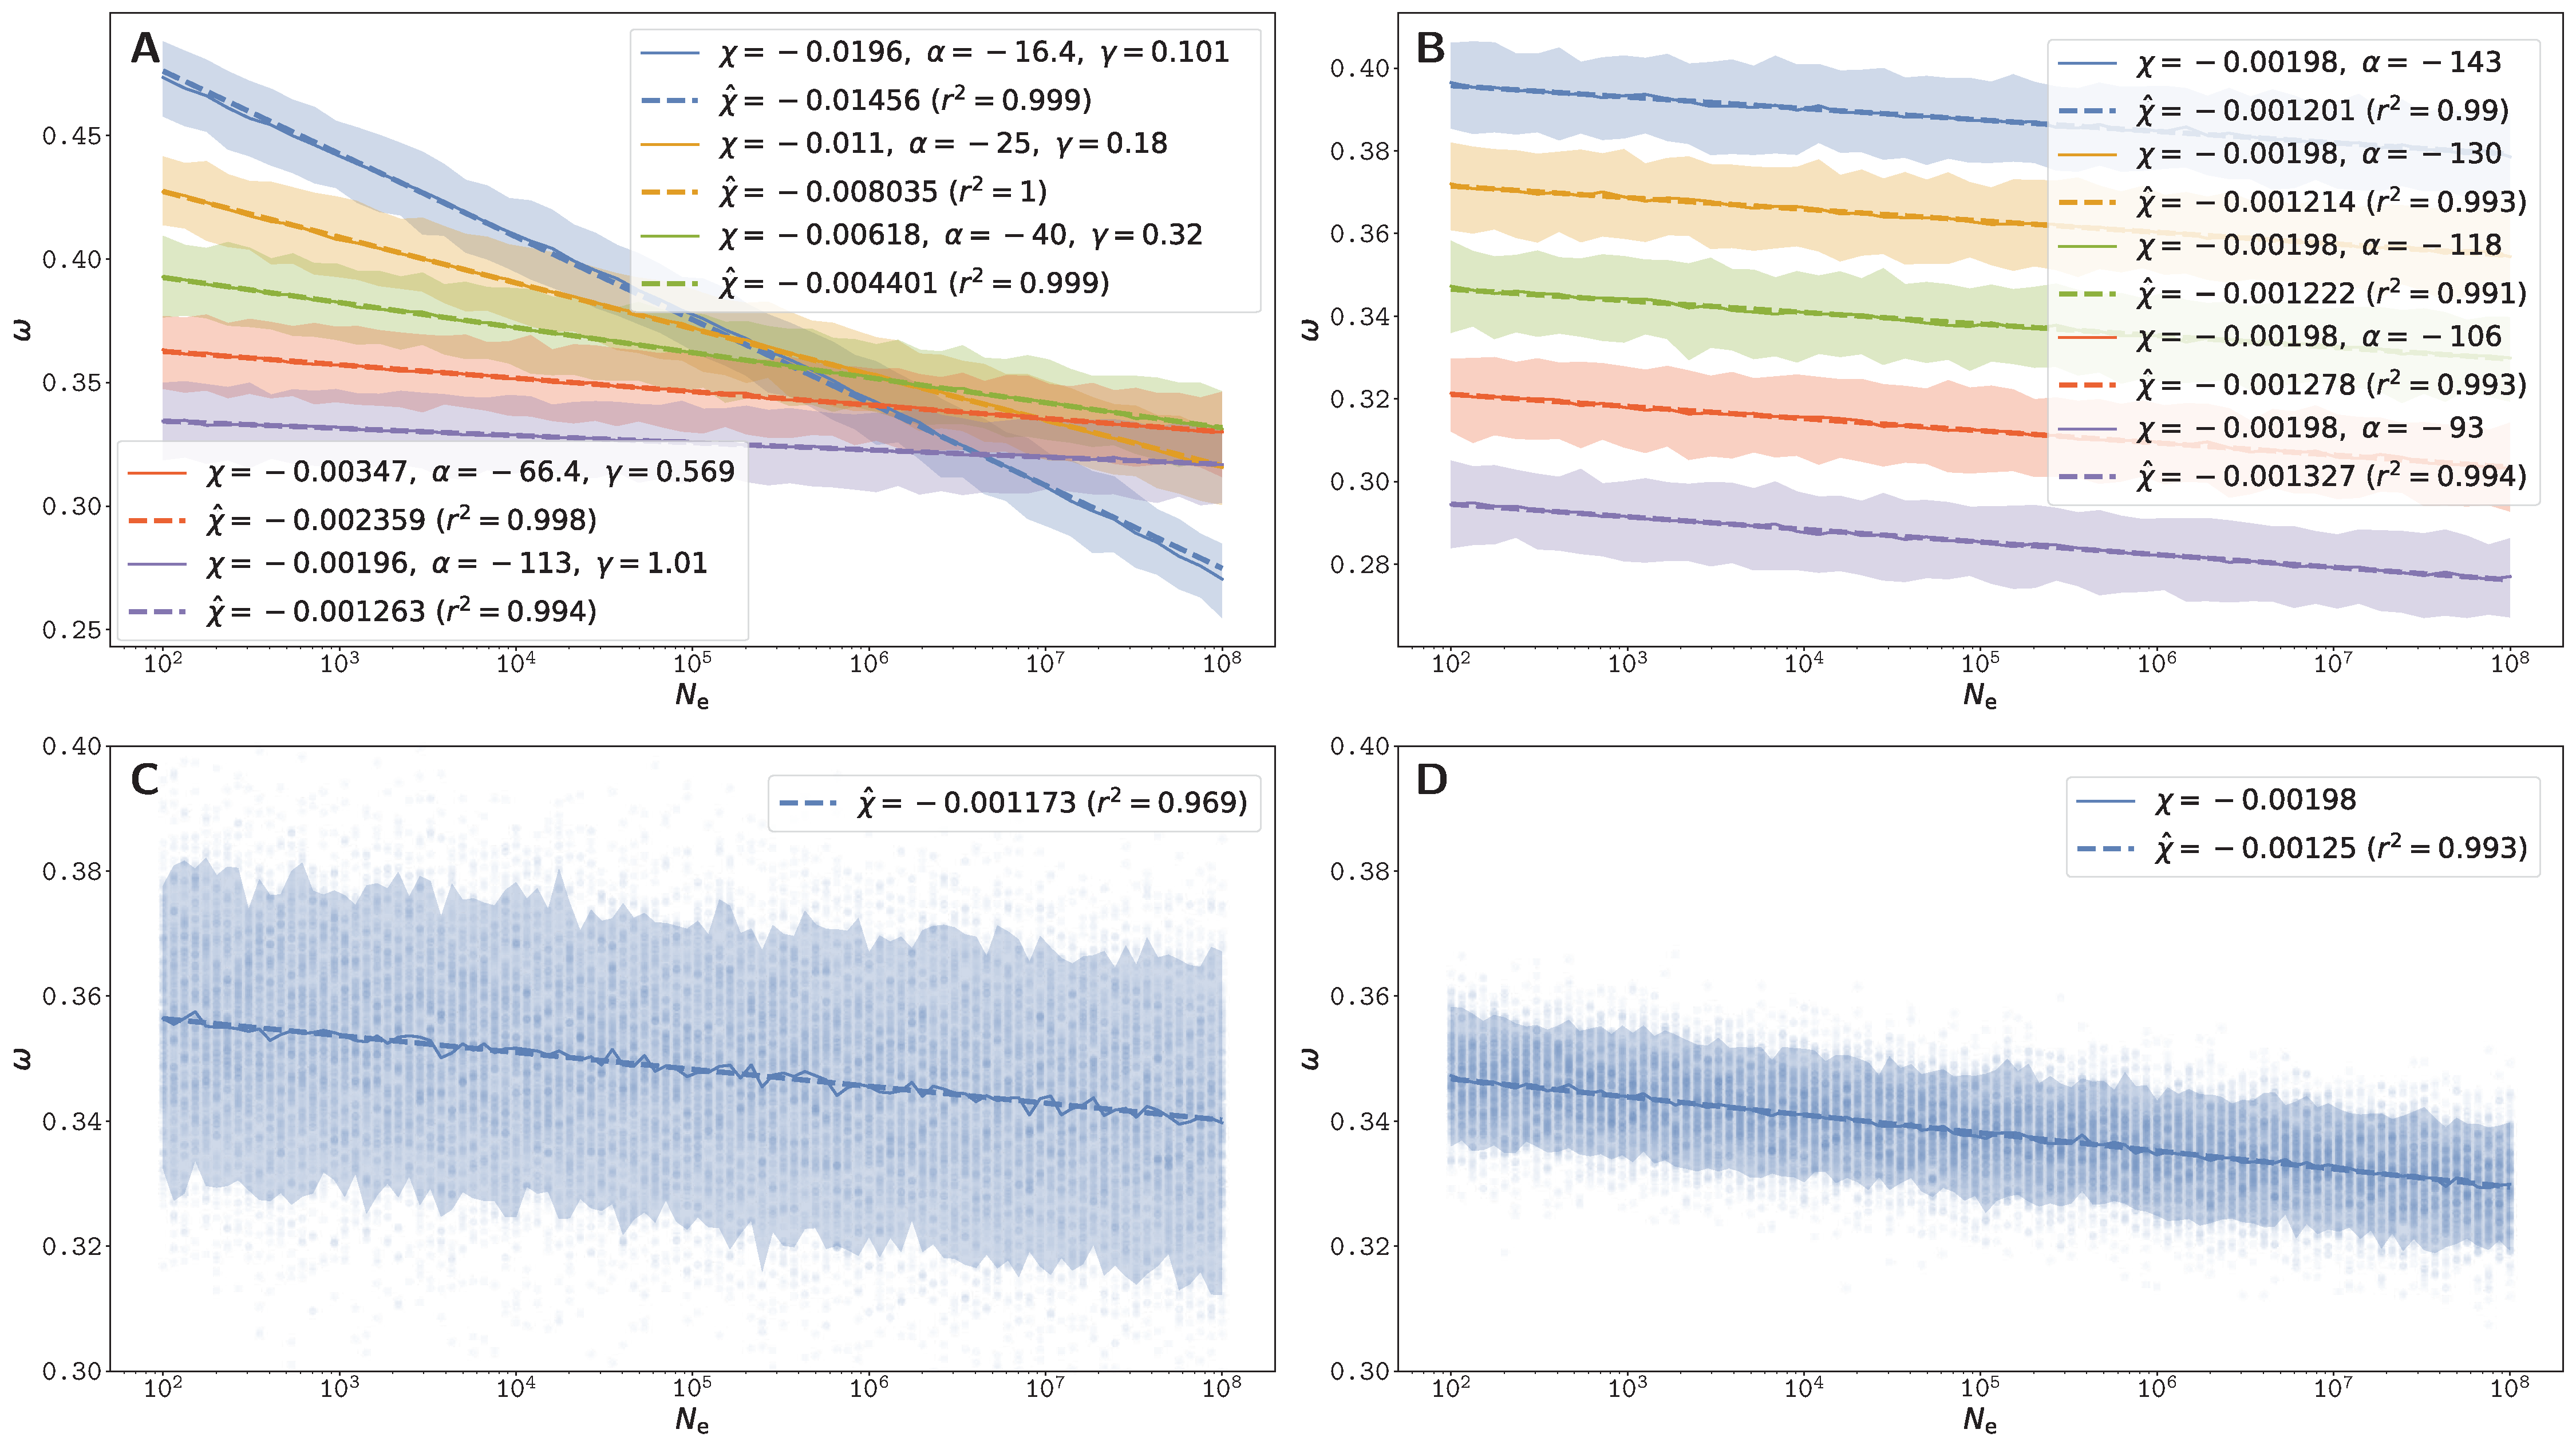
\includegraphics[width=\textwidth] {elasticity-low.pdf}

    \caption[$\omega$ susceptibility to change in $\Ne$]
    {$\omega$ susceptibility to change in $\Ne$.
    Scaling experiment simulating sequence evolution and recording the average $\omega$ in the vertical axis observed at equilibrium as a function of $\Ne$ in the horizontal axis.
    Along the x-axis, $200$ replicate simulations are performed for each different $\Ne$, the average (solid lines) and $90\%$ confidence interval (shaded area) of $\omega$ are shown.
    Linear regression (dashed lines) allows to estimate the susceptibility ($\hat{\chi}$), which is compared to theoretical expectation.
    The fixed parameters are $\NbrSites=300$, $\beta=1.686$.
    Simulations are conducted under our additive phenotype model (expect panel C), and for each non-optimal amino acid, $\DeltaDeltaG$ is scaled by the Grantham distance to the optimal amino acid.
    Panel A; $\DeltaGmin$ and $\DeltaDeltaG$ are given in the legend.
    $\DeltaDeltaG$ is increased and $\DeltaGmin$ is changed accordingly such that the equilibrium value $\smash{x\eq}$ is kept constant, by solving numerically equation~\ref{eq:equilibrium}.
    The estimated susceptibility ($\hat{\chi}$) decreases proportionally to the inverse of $\DeltaDeltaG$, as predicted by our theoretical model.
    Panel B; $\DeltaDeltaG=1$ and $\DeltaGmin$ are given in the legend.
    Decreasing $\DeltaGmin$ (to more negative values) increases $\omega$ but changes hardly the slope of the linear regression, as expected theoretically.
    Panel C; Folding free energy that determines the stability of the folded native state is computed using 3D structural conformations and pairwise contact potential energies between neighbouring amino-acid residues.
    The estimated susceptibility $\hat{\chi}$ is $-0.00124$, and as a result $\omega$ at equilibrium is weakly dependent on log-$\Ne$.
    Panel D; Simulation under the approximation of an additive free energy model, with empirical estimate of $\DeltaGmin = -118$ kcal/mol and $\DeltaDeltaG = 1$ kcal/mol.
    Our theoretical prediction of the susceptibility is $\chi = 0.00198$, close to the observation using 3D structural conformations.
    Under such parametrization, the scaling behaviour is similar to panel C, although with less variance.
    \label{fig:GoldsteinVsToy}
    }
\end{figure}

\subsection{Time to relaxation}

Although the equilibrium value of $\omega$ after changes in $\Ne$ is an important feature of the $\omega$-$\Ne$ relationship, another characteristic that is scarcely studied is the dynamic aspect~\citep{Jones2016}, particularly the relaxation time to reach the new equilibrium $\omega$.
We observed in our simulations that the determining factor of the relaxation time is the number of sites $\NbrSites$ (figure~\ref{fig:relaxStability}A), such that the return to equilibrium is faster for longer sequences.
This observation matches the theoretical prediction that more mutational opportunities are available for longer sequences, driving the trait close to equilibrium at a faster rate.

It may be useful to compare the relaxation pattern observed here with the predictions under two alternative models of sequence evolution, representing two extreme scenarios.
On one hand, having fitness modelled at the level of sites, such as contemplated by many phylogenetic mutation-selection models~\citep{Halpern1998, Rodrigue2010, Tamuri2012}, leads to a situation where every site has to adapt on its own to the new change in $\Ne$.
The relaxation time is then very long, on the order of the inverse of the per-site substitution rate.
On the other hand, assuming a fixed distribution of fitness effect (\acrshort{DFE}) as in \citet{Welch2008}, the response of $\omega$ is instantaneous (figure~\ref{fig:relaxStability}B).
Our model is effectively in between these two extreme scenarios.

Another characteristic observed in these non-equilibrium experiments is the discontinuity of $\omega$ after a change in $\Ne$.
Most importantly, both an increase and decrease in $\Ne$ lead to a discontinuity (figure~\ref{fig:relaxStability}A \&~\ref{fig:relaxStability}B).
These non-equilibrium behaviors can both be explained mechanistically.
Under low $\Ne$, the phenotype is far away from the optimal phenotype because the efficacy of selection is weaker.
A sudden increase in $\Ne$ results first in a short traction toward a more optimal phenotype, which results in a suddenly higher $\omega$, caused by a transient adaptation of the protein toward a higher stability.
Conversely, under high $\Ne$ the phenotype is closer to optimal and the purification of deleterious mutations is stronger.
The reaction to a decrease in $\Ne$ is a relaxation of the purification and thus an $\omega$ closer to the neutral case, which results into higher $\omega$ until reaching the point of marginal stability.
To note, an increase in $\Ne$ can theoretically and possibly lead to an $\omega$ that is temporarily greater than 1 due to adaptive evolution~\citep{Jones2016}, while a decrease in $\Ne$ always imply an $\omega < 1$, as it gives at most a neutral regime of relaxed selection.
\begin{figure}[htbp]
    \centering
    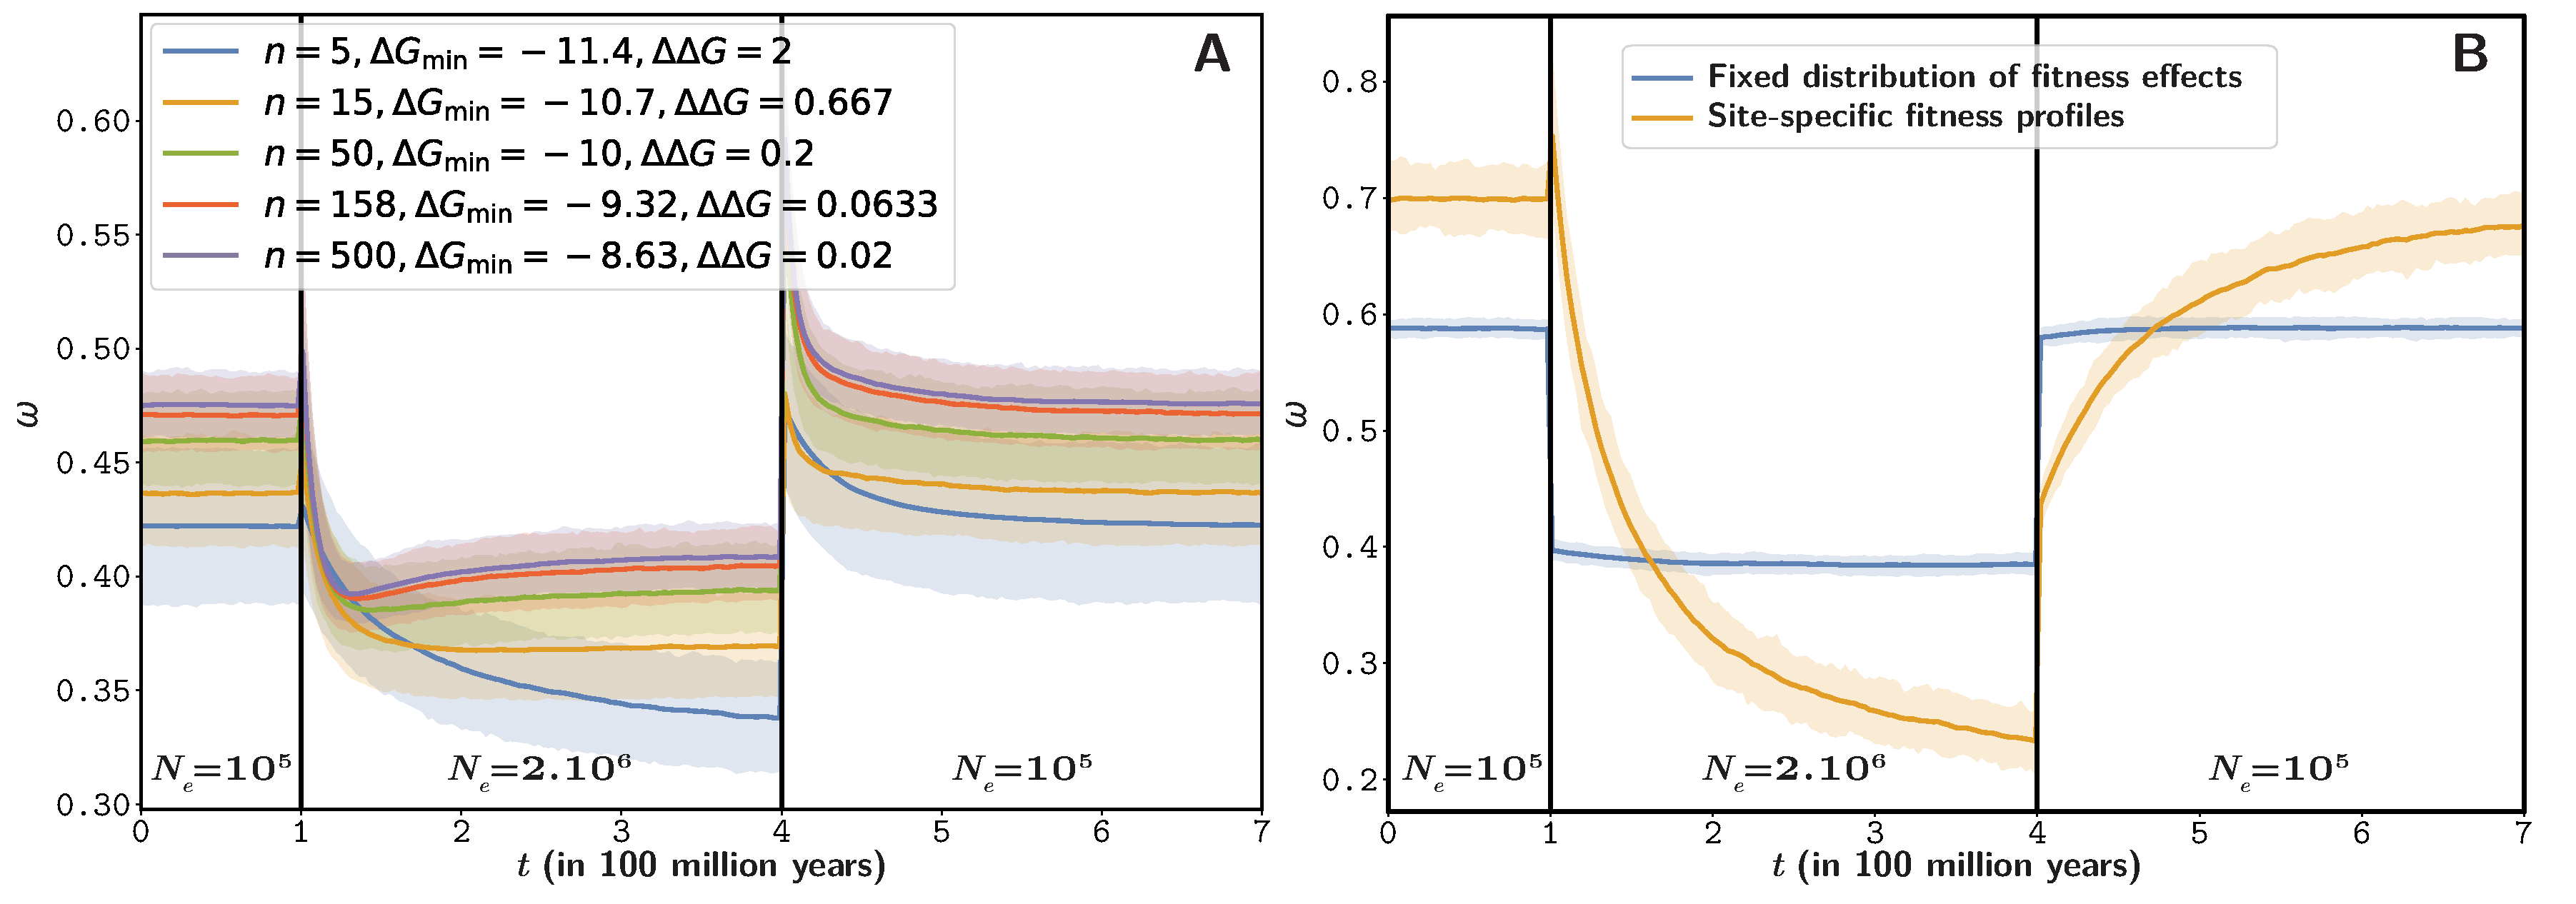
\includegraphics[width=\textwidth] {Relaxation.pdf}
    \caption[ $\omega$ relaxation after a change in $\Ne$]{
    $\omega$ relaxation after a change in $\Ne$.
    Solid line corresponds to the average over $1000$ replicates and the shaded area corresponds to the $90\%$ interval among replicates.
    The mutation rate ($\mu$) is $1e{-8}$ per year per site, and the total time of the computation is $700$ million years.
    Panel A.
    $\beta=1.686$ for all simulations.
    The \acrshort{DNA} sequence of $500$ sites is divided into exons of equal size.
    However the number of sites per exon changes between simulations from $\NbrSites=5$ to $\NbrSites=500$.
    Moreover, $\DeltaDeltaG$ is changed according to the exon size such that the product is kept constant, and as a consequence the susceptibility of $\omega$ to changes in $\Ne$ is kept constant.
    Finally, $\DeltaGmin$ is changed accordingly such that the equilibrium value $\smash{x\eq}$ is kept constant, by solving numerically equation~\ref{eq:equilibrium}.
    As such, whatever the exon size, $\smash{x\eq}$ and $\chi$ are kept constant and thus the observed effect is due to the number of sites in the exon.
    We observe that increasing the number of sites implies a reduced time to reach the new equilibrium.
    Panel B.
    In context of a time-independent fitness landscape, where each amino acid has different fitness (site-specific profile), the time taken to reach the new equilibrium value of $\omega$ after a change in $\Ne$ is long, such that relaxation rate is on the order of the mutation rate.
    In the context of a fixed distribution of fitness effects (\acrshort{DFE}), the relaxation time is non-existent and the new equilibrium value of $\omega$ is reached instantaneously.
    }
    \label{fig:relaxStability}
\end{figure}


\section{Discussion}
% Goal and theoretical results

We provide a compact analytical result for the equilibrium response (which, by analogy with thermodynamics, we call the susceptibility) of $\omega$ to changes in $\Ne$, and we relate this response to the parameterization of the genotype-phenotype-fitness map.
An application to a model of selection against protein misfolding shows that the susceptibility of $\omega$ to variation in $\Ne$ (in log space) is linear with a negative slope.
Furthermore, this application demonstrates that effective population size and protein expression level are interchangeable in respect to their impact on the response of $\omega$.
Our compact theoretical results, which were obtained by making several simplifying assumptions, are supported by more complex simulations of protein evolution relaxing these assumptions.
In particular, our theoretical predictions are verified under a numerical model of protein evolution in which the free energy is computed based on the 3D structure.

Overall, the susceptibility ($\chi$) is a function of structural parameters of the protein and takes a very simple analytical form, being is inversely proportional to the product of three terms;
namely the sequence size, the inverse temperature ($\beta$), and the average change in conformational energy of destabilizing mutations ($\EmpiricalDeltaDeltaG$).
Quantitatively, this product can be several orders of magnitude greater than $1$ in practice, such that the susceptibility of $\omega$, which is its inverse, is typically small.
Previous studies using this model presented an apparent lack of response of $\omega$ to changes in $\Ne$~\citep{Goldstein2013}.
We refine this result, by observing that there is in fact a very subtle and weak relation, which requires extensive computation to be detected, but which is well predicted by our theoretical derivation.
Based on empirical estimates of the structural parameters $\beta = 1.686$, $\NbrSites=300$ sites and $\EmpiricalDeltaDeltaG = 1.0$ kcal/mol~\citep{Zeldovich2007}, the estimated susceptibility is $\hat{\chi} \simeq -0.002$.
In other words, for a relative increase in $\Ne$ or expression level of $6$ orders of magnitude, a factor approximately equal $0.01$ is subtracted to $\omega$, a subtle relationship that requires laborious effort to be detected in simulated data.

\subsection{Adequacy to empirical data}
Empirically, variation in $\omega$ along the branches of phylogenetic trees has been inferred and correlated to proxies of $\Ne$, such as body size or other life-history traits.
These analyses showed mitigated support for a negative relation between $\omega$ and $\Ne$~\citep{Lanfear2014}.
More recently, phylogenetic integrative methods refined the estimate of covariation between $\omega$ and $\Ne$ along lineages by leveraging polymorphism data~\citep{Brevet2019}.
This approach gives an estimate of $\hat{\chi} \simeq 0.02$ in primates (section~\ref{sec:empirical-estimation-of-susceptibility} in supplementary materials) at least one order of magnitude greater than the quantitative estimate obtained above from the biophysical model.
More empirical data across different clades would be required to robustly consolidate such empirical estimates, but as of yet, these are challenging the idea of a very weak response.

% Stress the importance that susceptibility is valid for Ne and protein abondance
The relation between $\omega$ and expression level provides an independent, and potentially more robust, source of empirical observation.
Our theoretical results suggest that, under relatively general conditions, the response of $\omega$ to expression level should be of the same magnitude than the response to $\Ne$.
Empirically, protein expression level is one of the best predictors of $\omega$ and the empirical estimation of $\chi$ in fungi, archaea and bacteria varies in the range $[-0.046;-0.021]$ (table~\ref{tab:table-susceptibility} in supplementary materials) extracted from \citet{Zhang2015}.
Estimation in animals and plants gives somewhat lower estimates, in the range of $[-0.026;-0.004]$, although still higher (in absolute value) than $-0.002$.

Additionally, another empirical observation is the negative relation between the mean destabilizing effect of mutations (mean $\EmpiricalDeltaDeltaG$) and the $\DeltaG$ of the protein.
Such a relation is empirically observed in \citet{Serohijos2012}, with the slope of the linear regression ($\widehat{\rho}_{\EmpiricalDeltaDeltaG, \DeltaG}$) equal to $ = -0.13$.
The slope of the linear correlation observed in our simulations is weaker, with a slope of $\widehat{\rho}_{\EmpiricalDeltaDeltaG, \DeltaG} = -0.01$ under the 3D biophysical model, and $\widehat{\rho}_{\EmpiricalDeltaDeltaG, \DeltaG} = -0.003$ under the model of additive phenotype parameterized by $\DeltaDeltaG = 1$ and $\NbrSites=300$ (figure \label{fig:DG-vs-DDG} in supplementary materials).
This observation also sheds light on the correlation between $\omega$ and $\Ne$ in empirical data and in our model.
Indeed, equimutability, or namely that the distribution of $\EmpiricalDeltaDeltaG$ is independent of $\DeltaG$ is a necessary condition to observe independence between $\omega$ and $\Ne$~\citep{Cherry1998}.
In our model, $\EmpiricalDeltaDeltaG$ depends on $\DeltaG$ due to combinatorial considerations, but this dependence is weaker than empirically observed, which also translates into a weaker susceptibility of $\omega$ to changes in $\Ne$ or expression level than empirically observed.

Thus, overall, the response of $\omega$ to either $\Ne$ or expression level predicted by the biophysical model considered above seems lower than what is empirically observed.
There are several possible explanations for this discrepancy.
First, the biophysical model might be valid, but the numerical estimates used for $\NbrSites$ or $\EmpiricalDeltaDeltaG$ could be inadequate.
A $\EmpiricalDeltaDeltaG$ of $1.0$ kcal/mol seems to correspond to empirical estimates~\citep{Zeldovich2007}.
On the other hand, the effective number of positions implicated in the trait might be smaller than the total number of residues in the protein.
In our model, all positions in the protein can in principle compensate for the destabilizing effect of a mutation at a particular position.
In practice, the number of sites susceptible to compensate each other is probably smaller, resulting in a stronger departure from equimutability.

Alternatively, the biophysical model considered here might be too restrictive.
Recent empirical studies have provided evidence against the hypothesis that the rate of sequence evolution is driven solely by the toxicity effect of unfolded proteins~\citep{Plata2017,Razban2019,Biesiadecka2020}.
Notably, the response of $\omega$ to changes in expression level has also theoretically been found to arise as a consequence of protein-protein interactions, where protein may either be in free form or engaged in non-specific interactions~\citep{Yang2012, Zhang2013}.
In non-specific interactions at the protein surface, stabilizing amino acids are hydrophilic and destabilizing amino acids are hydrophobic, sticking to hydrophobic residues at the surface of other proteins~\citep{Dixit2013,Manhart2015}.

Our theoretical results can be applied more broadly to protein-protein interactions using a mean-field argument (section~\ref{sec:model-of-protein-protein-interactions} in supplementary materials).
Fitting this model with empirical structural estimates~\citep{Janin1995a, Zhang2008}, we obtain a susceptibility of $\chi \simeq -0.2$ thus a much stronger response than under the model based on conformational stability.
This much stronger response is due to fewer sites in the protein being involved in protein-protein interaction than for conformational stability, in addition to a lower free energy engaged in contact between residues.

Altogether, fitness based on protein stability is a compelling model of molecular evolution, but may not be a sufficiently comprehensive model to explain the amplitude of variation of $\omega$ empirically observed along a gradient of either effective population size or protein expression level.
The net response of $\omega$ to changes in $\Ne$ or expression level could have several biophysical causes, which in the end would imply a weak but still empirically measurable response.

\subsection{Physically grounded modelling}
% Analogy to physics
This study describes the signature imprinted on \acrshort{DNA} sequences by an evolutionary process by merging equations from population genetics and from structural physicochemical first principles.
Hence, physicochemical vocabulary and theory are recruited to describe the molecular details.
More widely, our modelling is imprinted with vocabulary and analogy to physical systems, with wording in the likes of forces, susceptibility and dynamic.
We argue that the analogy between evolutionary and physical systems is not restricted to wording, but allows one to visualize and intuit the causality chain and which approximation can be made in order to derive analytically tractable results~\citep{Sella2005, Mustonen2009, Bastolla2012, Bastolla2017}.
The robustness of results can be assessed by computational implementations and simulations.
Computational models offer a means to test the validity and robustness, while mathematical models offer an intuitive mechanistic mental analogy.

% Thermodynamic analogy
% Analogy to Clapeyron formula ? TdP/dT = d²H/d²V, where T is analogous to Ne
A first analogy between evolutionary biology and physics comes from statistical mechanics, describing how observable macroscopic properties are emerging from microscopic states.
As an example, in the Ising model, the magnetization is a macroscopic outcome of all microscopic atomic spins that can be in one of two states~\citep{Brush1967}.
At equilibrium when the system reaches minimum potential energy, the observable magnetization is controlled by variables such as temperature, and by external forces such as the magnetic field forcing the system.
By analogy, our atoms are sites of the sequence which can be in stabilizing or destabilizing state, and the macroscopic emerging observable is the relative substitution rate of selected mutation ($\omega$), which is controlled by effective population size ($\Ne$) analogous to temperature~\citep{Sella2005}.
Ultimately, the susceptibility of macroscopic observable ($\omega$) to a control variable ($\Ne$) can be tied to the microscopic parameters.
Another example of observable macroscopic properties, though not considered in this manuscript, could be for example site entropy, i.e. the effective number of observed amino acids per site at equilibrium~\citep{Goldstein2016, Jimenez2018, Jiang2018}.

% Mechanical analogy
% Elasticity with springs ? Surface tension with molecule and radius of the
% Elasticity ? Susceptibility (dimensionless) ? Compliance (units of metres per newton) ? Flexibility (units of metres per newton) ?
A second analogy between evolutionary biology physics comes from mechanics.
The phenotypic space is analogous to a spatial coordinate of the system, which is determined by external evolutionary forces; namely mutation, selection and drift.
These evolutionary forces are analogous to springs attached and stretching the phenotype in various directions and with various stiffness, resulting in an equilibrium point.
Once the equilibrium point is determined, an elastic (or reversible) deformation of the phenotype can be studied whenever applying a differential stress to the system.
In this analogy, changing the free energy of the reference phenotype ($\EmpiricalDeltaGmin$) leads in first approximation to changes of reference and equilibrium points but not a change in the stiffness of the springs, meaning the elastic coefficient (analog to susceptibility) is approximately conserved.
Conversely, stiffness ot the springs increases with regards to $\EmpiricalDeltaDeltaG$, meaning a that change in the stress applied to the system ($\Ne$) result in a weak deformation at the new equilibrium.

% Fundation to integrate other forces
Altogether, these analogies could be further formalized and used as a framework in which to integrate other external evolutionary forces.
Additional molecular processes could be included, for instance mutational bias, or GC-biased gene conversion inducing a bias in nucleic composition of genomes.
The change in equilibrium composition due to GC bias, and the magnitude of the response, could be investigated, such as to describe their signatures observable on molecular sequence, factoring the effects of mutation, selection and drift.
Finally, we hope that the results presented in this work, and more broadly the framework outlined here, could foster a better understanding of observable signatures of the long-term evolutionary process emerging from ecological parameters and molecular physicochemical first principles.

\subsection{Building block of inference models}

% Categories of models
At the crossroad between empirical data and theoretical models, inference models can compute the likelihood of an observation given a model, and also extract interpretable signature from molecular dataset.
Models of inference are classified broadly into phenomenological and mechanistic~\citep{Rodrigue2010a}.
Mechanistic models dissect the causation chains and construct a model from first principles, while phenomenological models aims to capture statistical aggregates (such as mean substitution rates) from the data.

% Phenomenological models
Example of such phenomenological models are the models parameterized directly in $\omega = \dnds$.
They will for example tell us which branch of the tree, or which site of the sequence has a decrease or increase in $\omega$ but not the underlying reason for such changes, which can be either mutation, selection, drift or another evolutionary force.
For example, in such models, a mutation and its reverse mutation do not have the opposite selection coefficient.
As such they cannot disentangle the potentially confounding effect of mutation, selection and drift.
Neither can they predict the nature of the functional relationship between population genetics or structural physicochemical parameters to $\omega$.

% Site specific mechanistic models of evolution
In contrast, mechanistic models relate structural, population-genetics and ecological parameters to the likelihood function.
As such, mechanistic inference models are suitable to construct an integrative framework relating the signal available in molecular sequences to structural parameters ($\EmpiricalDeltaDeltaG$), expression level across genes and effective population size across lineages.
Once such models are fitted to the data, the estimated parameters can be confronted to their independent empirical estimate ($\EmpiricalDeltaDeltaG, \Ne, \hdots$), which allows one to robustly test the model since orthogonal estimation of biological and ecological parameters should be congruent~\citep{Dasmeh2014}.
Additionally, once model robustness has been assessed, this inference framework could allow one to estimate unknown variables, for example ancestral effective population sizes, with enough signal and calibration of the other parameters.
Altogether, we argue that our theoretical results are a building block to construct an integrated inference framework of molecular evolution, since such models are bridging intrinsic biological parameters and the signal extractable from molecular sequences.


\section{Materials \& Methods}
Protein sequence evolution is simulated under an origin-fixation model~\citep{McCandlish2014}, where one sequence represents the whole population.
From the resident \acrshort{DNA} sequence $\Seqi$, we define $\setSeqNeighbors$ as the set of all possible mutant that are one nucleotide away from $\Seqi$, and were mutant sequences containing a stop codon are excluded.
For a protein of $\NbrSites$ amino-acid sites, $\left| \setSeqNeighbors \right| \leq 9 \NbrSites$, since each codon has a maximum of $9$ possible mutant codons that are one mutation away and that are not stop codon.
For each mutant sequence $\Seqj \in \setSeqNeighbors$, we compute its fitness and subsequently the selection coefficient of the mutant:
\begin{align}
    s \left( \Seqi,\Seqj\right) & = \dfrac{ \wrightfit \left(\Seqj \right) - \wrightfit \left(\Seqi\right) }{ \wrightfit \left( \Seqi\right)}, \\
    \Rightarrow s \left( \Seqi,\Seqj\right) & \simeq  \logfit \left(\Seqj \right) -   \logfit \left(\Seqj \right),
\end{align}
where $\wrightfit$ is the Wrightian fitness for a given phenotype and $\logfit $ is the Malthusian fitness (or log-fitness).

The next event of mutant invading the population, and the time to reach such event is chosen using Gillespie's algorithm~\citep{Gillespie1977}, according to the rates of substitution between sequences:
\begin{equation}
    \submatrix_{\Seqitoj} = \mu_{\Seqitoj} \dfrac{4 \Ne s \left( \Seqi,\Seqj\right)}{1 - \e^{-4 \Ne s \left( \Seqi,\Seqj\right)}},
\end{equation}
where $\mu_{\Seqitoj}$ is the mutation rate between $\Seqi$ and $\Seqj$, determined by the underlying $4x4$ nucleotide mutation rate matrix, and ${\submatrix_{\Seqitoj}} = \mu_{\Seqitoj}$ in the case of synonymous substitutions.
Various optimizations are implemented to reduce the computation time of mutant fitness.
The simulation starts with a burn-in period to reach mutation-selection-drift equilibrium.

\subsection{Models of fitness function}
\label{MatMet:folding}

Under a simulation of protein folding with an additive model of free energy, the protein's difference in free energy between folded and unfolded state is given by:
\begin{equation*}
    \DeltaG\left(\Seqi\right) = \DeltaGmin + \NbrSites \DeltaDeltaG * x\left(\Seqi\right),
\end{equation*}
where $0 \leq x\left(\Seqi\right) \leq 1$ is the distance of $\Seqi$ to the optimal sequence.
For each site of sequence, the optimal amino acids are chosen randomly at initialization, and the distance between the current amino acid and the optimal is scaled by the Grantham amino-acid distance~\citep{Grantham1974}.
Wrightian fitness is defined as the probability of our protein to be in the folded state, given by the Fermi-Dirac distribution:
\begin{equation}
    \wrightfit (\Seqi) = \dfrac{e^{-\beta \DeltaG\left(\Seqi\right) }}{1 + e^{-\beta \DeltaG\left(\Seqi\right) }} = \dfrac{1}{1 + e^{\beta \DeltaG\left(\Seqi\right) }},
\end{equation}
where $\beta$ is the inverse of the temperature ($\beta=1/kT$).

Under a simulation with site-specific fitness profiles, the protein log-fitness is computed as the sum of amino-acid log-fitnesses along the sequence.
In this model, each codon site $\i$ has its own fitness profile, denoted $\Profile^{(i)} = \{ \Profile^{(i)}_{\aaSource}, \forall 1 \leq \aaSource \leq 20 \}$, a vector of 20 amino-acid (Wrightian) fitnesses.
Since $\Seqi[ \i ]$ is the codon at site $\i$, the encoded amino acid is $\aaMap \left( \Seqi[ \i ] \right)$, hence the fitness at site $\i$ is $\Profile^{(i)}_{\aaMap \left( \Seqi[ \i ] \right)}$.
Altogether, the selection coefficient of the mutant $\Seqj$ is:
\begin{equation}
    s \left( \Seqi,\Seqj\right) = \sum\limits_{1 \leq \i \leq \Nsite} \ln \left( \dfrac{\Profile^{(i)}_{\aaMap \left( \Seqj[ \i ] \right)}}{\Profile^{(i)}_{\aaMap \left( \Seqi[ \i ] \right)}} \right),
\end{equation}
where $\Profile_{\i}$ used in this study are extracted from \citet{Bloom2017}, empirically determined in the context of deep mutational scanning.

Under simulation with a fixed distribution of fitness effects (\acrshort{DFE}), the selection coefficient of the mutant $\Seqj$ is gamma distributed (shape $k > 0$):
\begin{equation}
    - s \left( \Seqi,\Seqj\right) \sim \text{Gamma} \left( \bar{|s|}, k \right)
\end{equation}

\subsection{\texorpdfstring{$\omega$}{ω} along the simulation}
From the set of mutants $\setSeqNeighbors$ that is one nucleotide away from $\Seqi$, we define the subsets $\setSeqNonSynNeighbors$ and $\setSeqSynNeighbors$ that are respectively the set of non-synonymous and synonymous mutants, where $\setSeqNonSynNeighbors \cup \setSeqSynNeighbors = \setSeqNeighbors$.
As in previous works~\citep{Spielman2015, DosReis2015, Jones2016}, the ratio of non-synonymous over synonymous substitution rates of the sequence is defined as :
\begin{align}
    \omega(t) &= \dfrac{\sum\limits_{\Seqj \in \setSeqNonSynNeighbors} \submatrix_{\Seqitoj}}{\sum\limits_{\Seqj \in \setSeqNonSynNeighbors} \mu_{\Seqitoj}} \left( \dfrac{\sum\limits_{\Seqj \in \setSeqSynNeighbors} \submatrix_{\Seqitoj}}{\sum\limits_{\Seqj \in \setSeqSynNeighbors} \mu_{\Seqitoj}} \right)^{-1}\\
    &= \dfrac{\sum\limits_{\Seqj \in \setSeqNonSynNeighbors} \mu_{\Seqitoj} \dfrac{4 \Ne s \left( \Seqi,\Seqj\right)}{{1 - \e^{-4 \Ne \left( \Seqi,\Seqj\right)} }}}{\sum\limits_{\Seqj \in \setSeqNonSynNeighbors} \mu_{\Seqitoj}}
\end{align}
Averaged over all branches of the tree, the average $\omega$ is :
\begin{align}
    \omega & = \left\langle \omega(t) \right\rangle, \\
    & = \int_{t} \omega (t) \der t,
\end{align}
where the integral is taken over all branches of the tree, while the integrand $\omega (t)$ is a piece-wise function changing after every point substitution event.


\part{Conclusion}
\label{part:discussion}
%\chapter{Discussion}

\section{Inferring demography with divergence and polymorphism data}

Less sensitive to assumption of no epistasis and static fitness landscape.
The first strategy is to augment information about interspecies conservation with information about genetic polymorphism.
\subsection{Model assumptions and definition}
\subsubsection{Assumptions}
\begin{itemize}
	\setlength\itemsep{-0.25em}
	\item Known species tree and gene tree, meaning no paralogs and/or horizontal transfers.
	\item No epistasis, meaning independence between sites.
	\item Each sites is assigned a fitness profile, meaning different site of the sequence can share the same fitness profile.
	\item Inside each fitness profile, the fitness of each amino-acids is estimated.
	\item $\Ne$, $u$ and $\tau$ are correlated Brownian processes, giving each branch of the tree different $\Ne$, $u$ and $\tau$ estimates.
\end{itemize}
\subsubsection{Wright-Fisher process for a single site}
The Wright-Fisher process describe the change in frequency of single polymorphic site with two alleles in a population over time.
The model makes the following assumptions:
\begin{itemize}
	\setlength\itemsep{-0.2em}
	\item Non-overlapping generations
	\item Constant population size in each generation
	\item Random mating
\end{itemize}
Consider a population of $\Ne$ diploid individuals that has a single polymorphic site with two alleles, one ancestral (fitness = $1$) and one derived (fitness = $1+\selcoef$).
Assuming no dominance and no recurrent mutation, the probability, that there are $j$ copies of the derived allele present at generation $G+1$ (denoted $X_{G+1}$) given i copies of the derived allele present at generation $G$ (denoted $X_{G}$) is given by the following binomial calculation:
\begin{equation}
p\left( X_{G+1} = j |X_{G} = i, \Ne, \selcoef \right)  =  \binom{2 \Ne}{j} \left( \dfrac{x(1+\selcoef)}{x(1+\selcoef) + (1-x)} \right)^j \left(1 - \dfrac{x(1+\selcoef)}{x(1+\selcoef) + (1-x)} \right)^{2 \Ne -j}, 
\end{equation}
where $x = i / 2 \Ne$ is the derived allele frequency in generation $G$.\\
In this discrete framework, it has been shown to be extremely difficult to explicitly derive formulas for several quantities of evolutionary interest.
However, as the size of the population approaches infinity (i.e.
$ \Ne \rightarrow \infty$), and assuming that the scaled selection pressure ($\Ne \selcoef $) remain constant, the discrete Markov process given above can be closely approximated by a continuous-time, continuous-space diffusion process.\\
Under the assumption of no recurrent mutation, the derived allele with initial frequency $p$, goes either extinct ($x=0$) or fixed ($x=1$) after a long time.
It is possible to determine the probability of fixation ($p_{\mathrm{fix}}$), by using the Kolmogorov backward equation.
\begin{equation}
p_{\mathrm{fix}}(p, \scaledselcoef ) = \dfrac{1 - \e^{-\scaledselcoef p }}{1 - \e^{-\scaledselcoef}}\text{, where } \scaledselcoef=4\Ne \selcoef 
\end{equation}
\begin{figure}[H]
	\centering
	\begin{tikzpicture}
	\begin{axis}[
	ylabel={$p_{\mathrm{fix}}(p, \scaledselcoef )$},
	xlabel={Initial population frequency ($p$)},
	domain=0:1,
	cycle list name=colors,
	samples=100,
	legend entries={$\scaledselcoef=12$, $ \scaledselcoef=4$, $\scaledselcoef=0$, $\scaledselcoef=-4$, $\scaledselcoef=-12$},
	legend cell align=left,
	minor tick num=2,
	axis x line=bottom,
	axis y line=left,
	legend style={at={(0.1,0.9)},anchor=north west}
	]
	\addplot{(1 - exp(-12 * x)) / (1 - exp(- 12))};
	\addplot{(1 - exp(-4 * x)) / (1 - exp(- 4))};
	\addplot{x};
	\addplot{(1 - exp(4 * x)) / (1 - exp(4))};
	\addplot{(1 - exp(12 * x)) / (1 - exp(12))};
	\end{axis}
	\end{tikzpicture}
	\caption{\textbf{}}
\end{figure}
$g(x, \scaledselcoef) \der x $ is the expected time for which the population frequency of the derived allele, at the site, is in the range $(x, x+\der x)$ before eventual absorption:
\begin{align}
g(x, \scaledselcoef) & \approx  \dfrac{2 \left[ 1 - \e^{-\scaledselcoef (1-x)}\right]}{(1 - \e^{-\scaledselcoef})x(1-x)}
\end{align}
\begin{figure}[H]
	\centering
	\begin{tikzpicture}
	\begin{axis}[
	ylabel={$g(x, \scaledselcoef)$},
	xlabel={frequency of the derived allele ($x$)},
	domain=0.05:0.95,
	cycle list name=colors,
	samples=100,
	legend entries={$\scaledselcoef=12$, $ \scaledselcoef=4$, $\scaledselcoef=0$, $\scaledselcoef=-4$, $\scaledselcoef=-12$},
	legend cell align=left,
	minor tick num=2,
	axis x line=bottom,
	axis y line=left,
	legend style={at={(0.1,0.9)},anchor=north west}
	]
	\addplot{2 * (1 - exp(-12 * (1-x))) / ((1 - exp(-12))*x*(1-x))};
	\addplot{2 * (1 - exp(-4 * (1-x))) / ((1 - exp(-4))*x*(1-x))};
	\addplot{2 / x};
	\addplot{2 * (1 - exp(4 * (1-x))) / ((1 - exp(4))*x*(1-x))};
	\addplot{2 * (1 - exp(12 * (1-x))) / ((1 - exp(12))*x*(1-x))};
	\end{axis}
	\end{tikzpicture}
	\caption{\textbf{}}
\end{figure}
\subsubsection{Poisson random fields in Mutation-Selection framework }
S. Sawyer and D. Hartl expanded the modeling of site evolution to multiple sites.
The model makes the following assumptions: 
\begin{itemize}
	\setlength\itemsep{-0.2em}
	\item Mutations arise at Poisson times (rate $u$ per site per generation)
	\item Each mutation occurs at a new site (infinite sites, irreversible)
	\item Each mutant follows an independent Wright-Fisher process (no linkage)
\end{itemize}
In a sample of size $\samples$, the expected number of sites with $k$ (which ranges from $1$ to $\samples-1$) copies of the derived allele is defined as a function of $g(x)$:
\begin{align}
G(\copies, \samples, \theta, \scaledselcoef) & = 2 \Ne u \int_{0}^{1} g(x, \scaledselcoef)  \binom{\samples}{\copies} x^{\copies} (1-x)^{\samples-\copies} \der x \nonumber \\
& = \theta \int_{0}^{1} \dfrac{1 - \e^{-\scaledselcoef (1-x)}}{(1 - \e^{-\scaledselcoef})x(1-x)} \binom{\samples}{\copies} x^{\copies} (1-x)^{\samples-\copies} \der x\text{, where } \theta=4\Ne u \nonumber \\
& = \binom{\samples}{\copies} \dfrac{\theta }{1 - \e^{-\scaledselcoef}} \int_{0}^{1} \left( 1 - \e^{-\scaledselcoef (1-x)} \right) x^{\copies-1} (1-x)^{\samples-\copies-1} \der x
\end{align}
In the mutation selection-framework developed, the fitness of a given genotype is a function of the encoded amino-acid through the site-wise amino-acid fitness profiles ($ \Fit\siteexp $ at site $\site$). Thus the coefficient ($\scaledselcoef=4\Ne \selcoef $) associated to a mutation is a function of the amino-acids encoded by the ancestral ($\ci$) and derived ($\cj$) codon. Altogether the selection coefficient from $\ci$ to $\cj$ at site $\site$ is:
\begin{align}
\scaledselcoef_{\itoj}(\Ne, \Fit\siteexp) &= 4 \Ne (f_\cj\siteexp-f_\ci\siteexp) \nonumber \\
& = \scaledfit_\cj\siteexp-\scaledfit_\ci\siteexp
\end{align}
Similarly, the mutation rate between by the ancestral ($\ci$) and derived ($\cj$) codon is a function of the nucleotide changes between the codons. If the codons are not neighbor, meaning a single mutation is not sufficient to jump from $\ci$) to $\cj$, the mutation rate is equal to $0$. If the codons are neighbors, the mutation rate is given by the nucleotide rate matrix ($ \bm{u} $). Altogether, the scaled mutation rate $\theta_{\itoj}$ from $\ci$ to $\cj$ is:
\begin{equation}
\theta_{\itoj}(\Ne, u, \Mutmatrix) = 4 \Ne u \mutmatrix_{\itoj}
\end{equation}
If a site is polymorphic and the ancestral ($\ci$) and derived ($\cj$) codons are neighbors, the probability of observing $\copies$ copies ($\samples \geq \copies > 0$) of the derived codon ($\cj$), in a sample of size $\samples$, at site $\site$, is given by:
\begin{equation}
P(\ci=\samples-\copies,\cj=\copies \ |\ \Ne, u, \Mutmatrix, \Fit\siteexp)  =  G\left(\copies, \samples, \theta_{\itoj}(\Ne, u, \Mutmatrix), \scaledselcoef_{\itoj}(\Ne, \Fit\siteexp) \right)
\end{equation}
Moreover the probability that a site is monomorphic is given by:
\begin{equation}
P(\ci= \samples \ |\ \Ne, u, \Mutmatrix, \Fit\siteexp)  = 1 - \sum_{\cj \in \Ni} \sum_{\copies=1}^{\samples}  G\left(\copies, \samples, \theta_{\itoj}(\Ne, u, \Mutmatrix),  \scaledselcoef_{\itoj}(\Ne, \Fit\siteexp)\right)
\end{equation}
And all other probabilities equal to $0.0$.


\section{Complexity}

\subsection{Epistasis}

\subsection{$\omega_A$}


\section{The art of modeling}
I believe analytical models, computational simulations and inference models are complementary, but more importantly they are necessary to each others. 
Theoretical modeling allow to understand the principles, simulations allow to verify the soundness.
Inference allow to extract and test the theoretical results using empirical data.
Simulations have a dual role, testing the robustness of both inference procedures and theoretical results, outside of their comfort zone and assumptions.
However, this assume we are confident enough to write reproducible computations, as such the next section is dedicated to my experience and take away.

\subsection{Reproducible computations}
First, I stand firmly on the ground that data, codes and scripts should be rendered open-access of any published and peer reviewed paper.
Practically, the availability of the data and source code should simply be enforced upon submission to journal, which is currently not the case for many, even in bio-informatics and genomics fields.
This strong stance is not as to make scientist publish less, though it is a positive side-effect such as to be able to keep up with the literature.
On the contrary, is to avoid the bloating of what is called a technical debt, or research debt.
It encourages peer collaboration, both helping the team or person whom made the code available, and the community as a whole.
A straightforward way is to provide a git repository with the advantage that collaboration is facilitated trough web hosted repository such as GitLab or GitHub.

Test reproducing the results should also be made available, many tools are available to this aim.
When only python code is necessary for the reproductibility, anaconda/conda provides a straightforward environment to configure the necessary libraries with their versions. 
Jupyter notebooks also provide a 
For more complex environment, requiring compiling source code a more general environment is either a Docker or Singularity for example, but any containers implementing system-level virtualization is very helpful.
These tools are emerging in the community 


Workflow management system (Nexflow, Snakemake, etc) allowing to create reproducible and scalable data analyses.
Peer-coding sessions, continuous integration pipeline are valuable to use to increase the reliability of code generation.
 
\subsection{Bayesian statistics}
Knowing that maximum likelihood and Bayesian statistics are often opposed to each others and fiercely defended by their tenant I would gladly give my opinion on the matter, since I made the . 
Bayesian statistics seems personally a more comfortable inference framework than maximum likelihood for several reasons. 
First you do not need to care for local optimum which might freeze the program.
Second and most importantly, it gives the confidence interval, meaning how much certainty is available given the data on a estimate.
A corollary is that over parametrization is not an issue. 
Lasso or penalized-likelihood methods are not required.
The subjective arbitrary introduced by lasso and penalized-likelihood is replaced by statistical prior distribution, which are more meaningful.
Moreover, it gives a simple, thought extensive method to test for the repeatability and soundness of the code (cf prior distribution must match the rank).
Finally, the sampling method of 

\section{Reflecting on the mutation-selection-drift equilibrium}
In this section, I'll develop reflections on apparent similarities and analogies between the mutation-selection-drift process and other processes present in a variety of scientific fields, displaying the same underlying mechanism and emerging properties, though with different name and aspiration.
Such attempts requires to boil down the mutation-selection-drift mechanism into its core components, while at the same time rephrasing the description using lexicography outside of population-genetic such as to open new perceiving angles.

At the bottom, mutation is a process creating diversity, changing and moving the current viable state to a novel and unknown position, fundamentally allowing exploration of the state space.
On the other hand, selection is the criteria on which a new state is deemed a disrupting innovation or a nonviable alteration, and allow to determine which changes to exploit and which to filter out and discard based on its fitness.
Fundamentally, reducing the diversity created by the mutation process is the very essence of selection.
Finally, drift arbitrate between the creation and reduction of the two processes, it dictates how much exploration of novelty is permitted, and conversely how much exploitation of only the fittest states is granted.

I argue that this creation and reduction process is found at the core of several research disciplines, while the link between them is scarcely made \cite{Baeck1994, Eiben1998}. 

\subsubsection{Metropolis-Hasting sampling}
Obtaining a sequence of random samples from a probability distribution can be difficult, especially when the number of dimensions is high.
However, the Metropolis-Hasting procedure based on a Monte Carlo Markov chain can sample from any probability distribution, provided that we know how to compute the probability density, or even less restrictively any function proportional to the density \cite{Hastings1970}.
This stochastic procedure which is based on three steps bears many similarities with the mutation-selection-drift process:
\begin{itemize}
	\item Generate a stochastic candidate from the current state, analogous to the mutation.
	\item Calculate the acceptance ratio as the ratio of the two densities, analogous to the selection coefficient of the mutated state.
	\item Stochastic acceptance or rejection based on the acceptance ratio, a process analogous to drift. 
\end{itemize}
Inherently, is Metropolis-Hasting procedure is based on creating and subsequently reducing diversity, which allows to obtain a random sequence of samples from any distribution with a straightforward recipe, and is a critical tools in statistic and statistical physics.

\subsubsection{The exploration-exploitation dilemma}
Many mathematical, engineering and day-life problems are not about sampling a state space, but rather finding the optimal and best state given a criteria or a function to maximize.
Naturally, we would prefer deterministic (strictly reproducible) rather than stochastic optimizing strategies to be in searching the optimal state.
Unfortunately, whenever the state space is too large, often due to the curse of dimensionality, a greedy or heuristic search of an optimal state can performs atrociously \cite{Bellman1966}.
In high dimensional space, stochastic optimization tools have been deemed very valuable, such as stochastic gradient decent or so called evolutionary algorithm.
Inherently, they are based on two arms, one arm is stochastically creating diversity and exploring the state space, while the other arm is filtering the explored states and thus reducing the diversity.

In the constrained case of a finite number of time or attempt to find the best score overall, the problem is best described by the example of the multi-armed problem. The name comes from imagining a gambler at a row of slot machines (sometimes known as "one-armed bandits"), where each slot machine provides a random reward from a probability distribution specific to that machine. The player has to decide which machines to play, how many times to play each machine and in which order to play them, and whether to continue with the current machine or try a different machine, such as to maximize the sum of rewards earned through a sequence of lever pulls.
The gambler faces a dilemma at each trial, between "exploitation" of the machine that has the highest expected payoff and "exploration" to get more information about the expected payoffs of the other machines. 
The need to obtain new knowledge and the need to use that knowledge to improve performance is trade-off that need to be balanced to obtain an optimal performance.
As an example application of the exploration-exploitation procedure is AlphaGo, the first computational program mastering the board game go at the professional 9-dan level in 2017 and out-compete Ke Jie, the world n°1 ranked player at the time \cite{Silver2017, Silver2018}.
AlphaGo has often been publicized and hyped in various media outlets that this feat was possible due to machine learning, more specifically due to convolutionnal neural networks. However, it is more scarcely mentioned that AlphaGo neural networks is combined with an exploration-exploitation algorithm, or more specifically Monte Carlo tree search. 
In practice, the neural network is used as a criteria to measure the advantage of a board configuration,
but the different moves and path probed and trimmed is done via an exploration-exploitation procedure. 
As twist of fate, stochastic gradient descend (mentioned above), is a central algorithm to make the convolutionnal neural networks converge.

\subsubsection{In finance, economics, psychology and neurology}
Historically, there as been many bridges and crossover between economics and evolution.
For example game theory had originally been developed to model economic actors behavior and strategies \cite{Neumann1947}, while latter being incorporated into evolutionary biology to explain the emergence of altruistic behaviours in Darwinian evolution, the conundrum of the existence of the peacock's tail and other such biological encumbrances \cite{Smith1973, Smith1982}.
They are also analogous explanation between absolute and relative fitness \cite{Masel2016}.

The exploration-exploitation dilemma can be used to explain a multitude of phenomena, such as the movement of animals in novel landscapes, the most efficient resource allocation for a start-up company, or the effects of old age on knowledge acquisition in humans.
Of course, scientific research endeavor is also a exploration-exploitation dilemma, which in my personal feeling is externally pressured to pursue the exploitation at the risk of being 
Create and reduce, explore and exploit, mutate and select are different name that encompass the used when the sampling state is too large to be explored.
I argue that scientific fields studying and leveraging this pervasive process can gain knowledge with each others by interacting. 
As an example, I believe the methods developed in reinforcement learning, such as Monte Carlo tree search can help devise efficient inference procedure in molecular evolution. 
% As a side note, it appears that drift and selection are actually confounded, they are both on the side of exploitation, not on exploration.
% Sex and mutation are both generating new states and are part of the more general exploration facet.
% This explains why sex is favored in fluctuating environments.

\chapter*{Conclusion}
\addcontentsline{toc}{part}{Conclusion}
Drop in the ocean 

%% APPENDICES %% 
\part{Appendices}

\thispagestyle{empty}
\chapter{Inferring long-term population size - Supplementary Materials}
{\hypersetup{linkcolor=GREYDARK}\minitoc}
\label{chap:MutSelDrift-SuppMat}
\section{Summary statistics}

\subsection{Partial correlation coefficient}

The correlation coefficient $\rho_{\traiti, \traitj}$ give the total regression between two variable.
Partial-correlation coefficient account for the entire covariance matrix, and measure the correlation between $2$ traits, knowing the values of all the other traits:
\begin{equation}
    \rho_{\traiti, \traitj | c \in \traitInterval \setminus \{ a, b\} } = - \dfrac{\Precisionmatrix_{\traiti, \traitj}}{\sqrt{\Precisionmatrix_{\traiti, \traiti} \Precisionmatrix_{\traitj, \traitj}}},
\end{equation}
where the precision matrix $\PrecisionMatrix$ is the inverse of the covariance matrix:
\begin{equation}
    \PrecisionMatrix = \CovarianceMatrix^{-1}
\end{equation}

\subsection{Fitness profile entropy}
For a category $\cat$, the Shannon entropy ($\Omega$) of the fitness profile is defined as:
\begin{equation}
    \Omega \left( \Base\catexp \right) = - \sum_{\aSetAa} \base\catexp_{\aminoacid} \log \left( \base\catexp_{\aminoacid} \right)
\end{equation}
The Shannon entropy measures the flatness of the fitness profile, with a value of $0$ corresponding to a single peak fitness landscape (only one amino-acid is present), and a value of $log(20)\simeq3$ corresponding to a neutral landscape, where each amino-acid has the same fitness.

The Shannon entropy can be averaged out as:
\begin{equation}
    \langle \Omega \left( \Fit \right) \rangle = \dfrac{1}{\Ncat}\sum_{\Setcat} \Omega \left( \Base\catexp \right)
\end{equation}
The average Shannon entropy was obtained in a context of constant $\Ne$ along the tree, and compared with the experiment where $\Ne$ is allowed to vary according to a log-Brownian process.


\section{Simulations}

\subsection{Independent fitness profiles}
Under a simulation with site independent fitness profiles, a fitness profile give a fitness for each amino-acid (vector of size $20$).
Each site of the protein has a specific amino-acid fitness profile.
Overall, the protein fitness is computed as the sum of site-specific fitness, obtained by accessing the amino-acid present at each site of the protein.
For each possible mutant, we compute the selection coefficient of the mutant:
\begin{equation}
    s \left( \mathbb{S}^{t},\mathbb{S}^{t+1}\right) = \sum_{1 \leq \site \leq \Nsite} \ln \left( \dfrac{G_{\site} \left(\mathbb{S}^{t+1}(\site) \right)}{G_{\site} \left(\mathbb{S}^{t}(\site) \right)} \right),
\end{equation}
where $G_{\site}$ is the fitness profile at site $\site$, obtained in empirical experiment \citep{Bloom2017}.

\begin{center}
    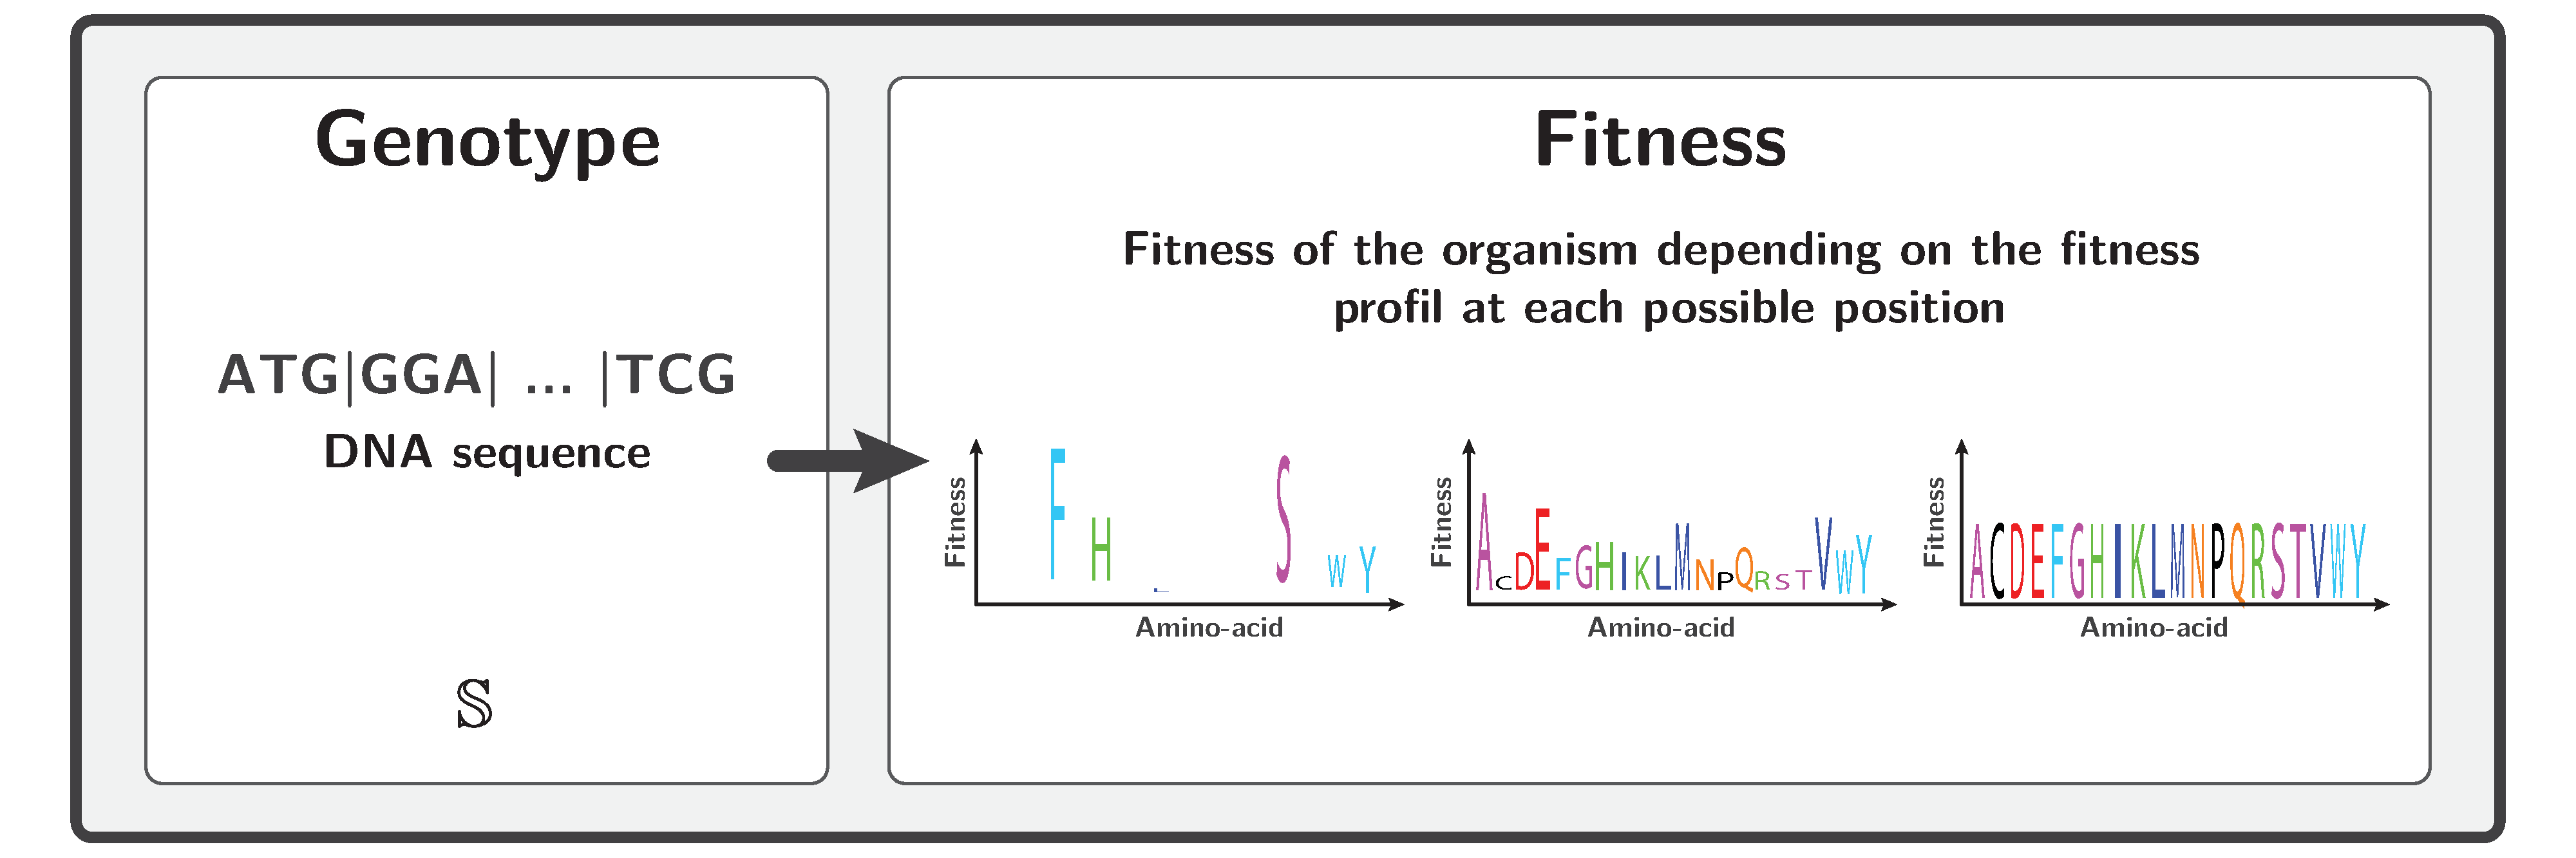
\includegraphics[width=\textwidth] {ModelSimuDiv}
\end{center}

The next change in the protein coding DNA and the time to next the event is chosen using Gillespie algorithm, according to the rates of substitution between codons:
\begin{equation}
{\submatrix_{\itoj}}
    = \mu_{\itoj} \dfrac{4 \Ne s \left( \mathbb{S}^{t},\mathbb{S}^{t+1}\right)}{{1 - \e^{-4 \Ne s \left( \mathbb{S}^{t},\mathbb{S}^{t+1}\right)} }},
\end{equation}
where ${\submatrix_{\itoj}} = \mu_{\itoj}$ in the case of synonymous substitutions.

\subsection{Wright-Fisher with polymorphism}

The evolutionary dynamics was formalized as a Wright-Fisher model with mutation, selection and drift. The population is assumed to be panmictic, with with effective population size $\Ne$ and with non-overlapping generations.

\begin{center}
    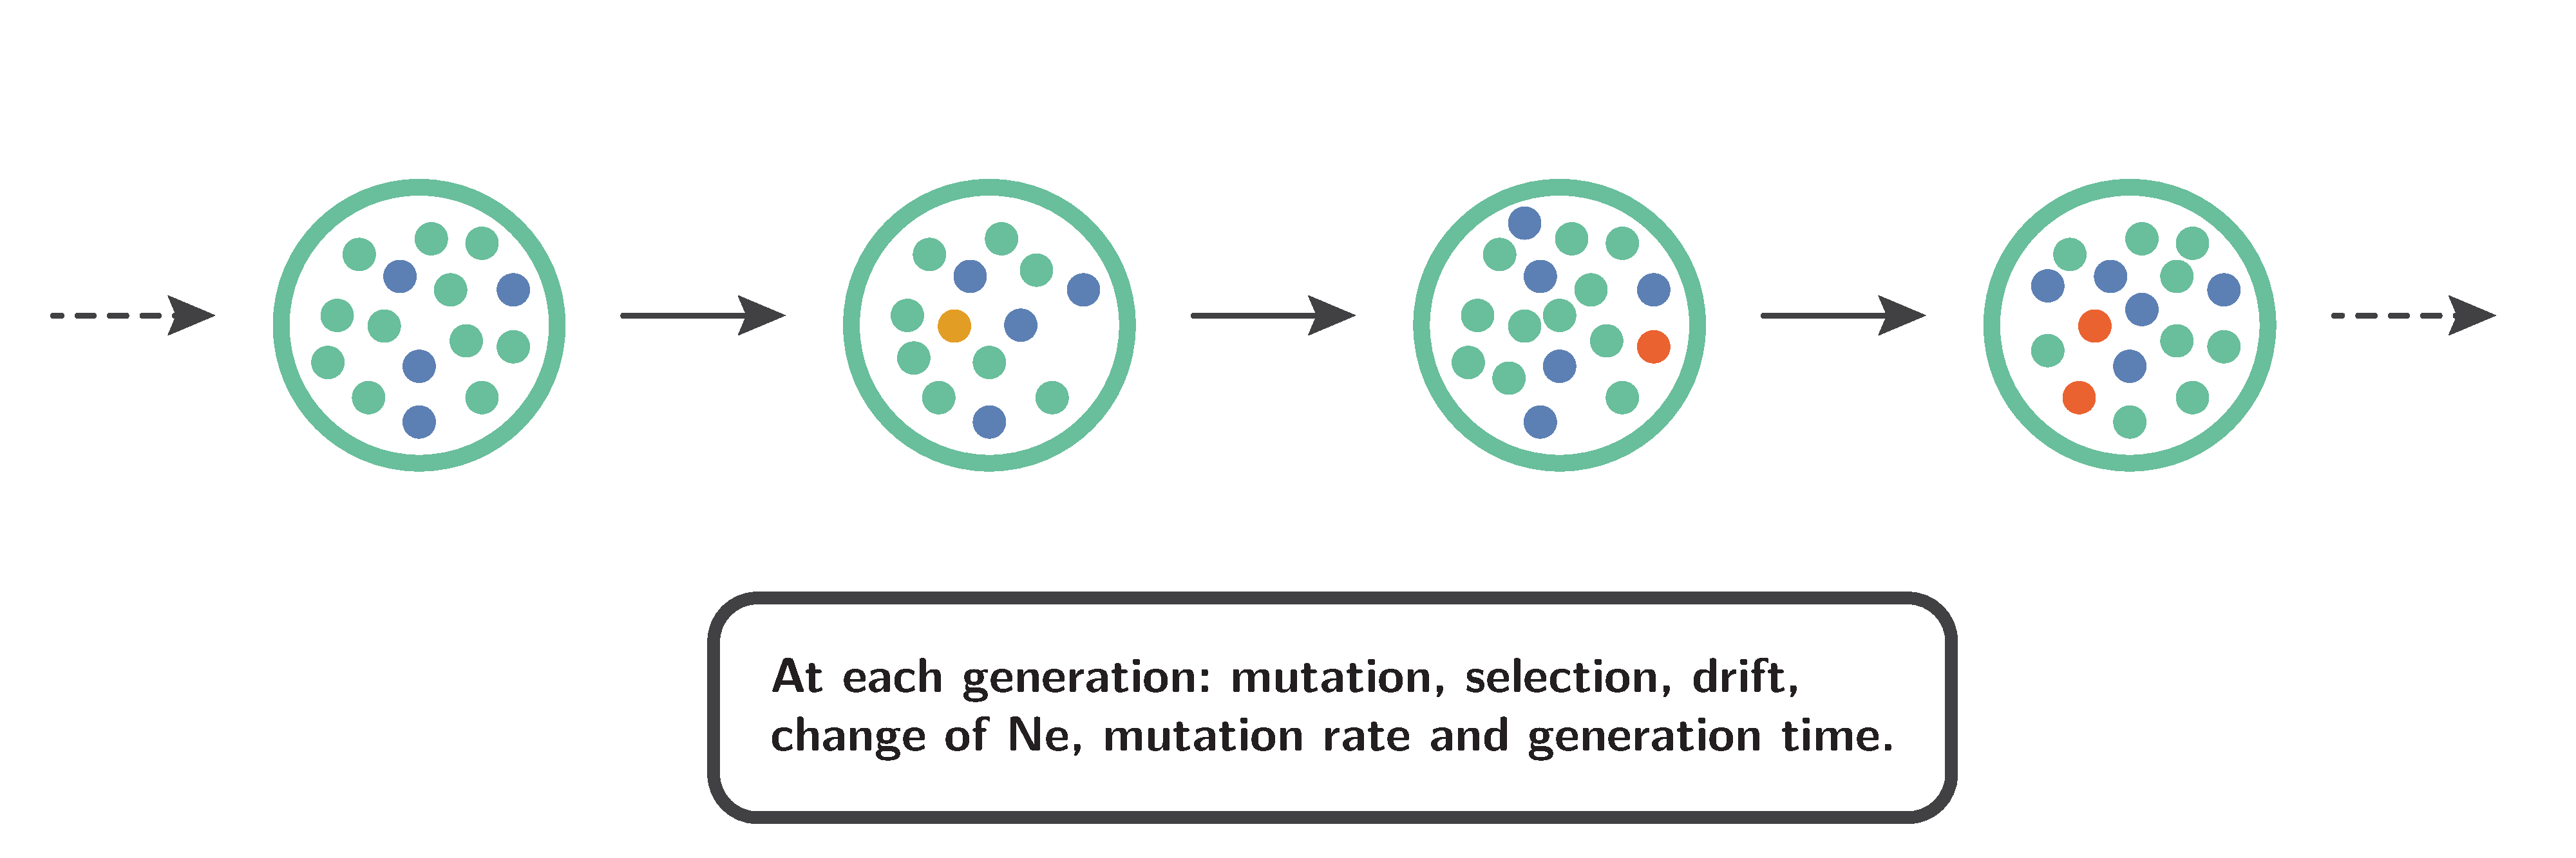
\includegraphics[width=\textwidth] {ModelSimuPoly}
\end{center}

\subsection{Fisher geometric landscape}

We simulated substitutions in a protein using an adaptation of Fisher's geometric landscape.
In the original context, the phenotype is a vector ($\phenoGeo$) in a multidimensional space, where the number of dimensions is often termed complexity.
From a phenotype, the fitness is a monotonously decreasing function of the phenotype distance to $0$.
The exact functional phenotype-fitness map depend on $2$ external parameters controlling for strength ($\alpha$) and epistasis ($\beta$).
If the phenotype-fitness map is explicit, the genotype-phenotype map is more pervasive.
Mutations are seen has displacement of the phenotype in the multidimensional space.
Beneficial mutations are moving the phenotype closer to $0$, whereas deleterious mutations are moving the phenotype further away.
In such original context, the distribution of mutational effects is not dependent on the current genotype, but this can be relaxed using a genotype-phenotype map.\\

In a protein context, the genotype-phenotype map can be defined by assigning to each of the $20$ amino-acid a vector in the multidimensional space.
Since different sites of the protein do not have the same physico-chimical properties, we can define a specific genotype-phenotype map for each position of the sequence.
Overall, the protein phenotype is computed as the sum of site-specific multidimensional vectors, obtained by accessing the amino-acid present at each site of the protein.
From a DNA sequence $\mathbb{S}^t$ after $t$ substitutions, the protein's phenotype is given by:
\begin{equation}
    \phenoGeo\left(\mathbb{S}^{t}\right) = \sum_{1 \leq \site \leq \Nsite} \phenoGeo_{\site} \left(\mathbb{S}^t(\site) \right),
\end{equation}
where $\phenoGeo_{\site}$ is the genotype-phenotype map at site $\site$.\\

And the Wrightian fitness of $\mathbb{S}^t$ is :
\begin{equation}
    w\left( \phenoGeo\left(\mathbb{S}^{t}\right) \right) = e^{-\alpha \left| \phenoGeo\left(\mathbb{S}^{t}\right) \right|^{\beta}},
\end{equation}
where strength ($\alpha > 0$) and epistasis ($\beta$) are parameters of the fitness function.
\begin{center}
    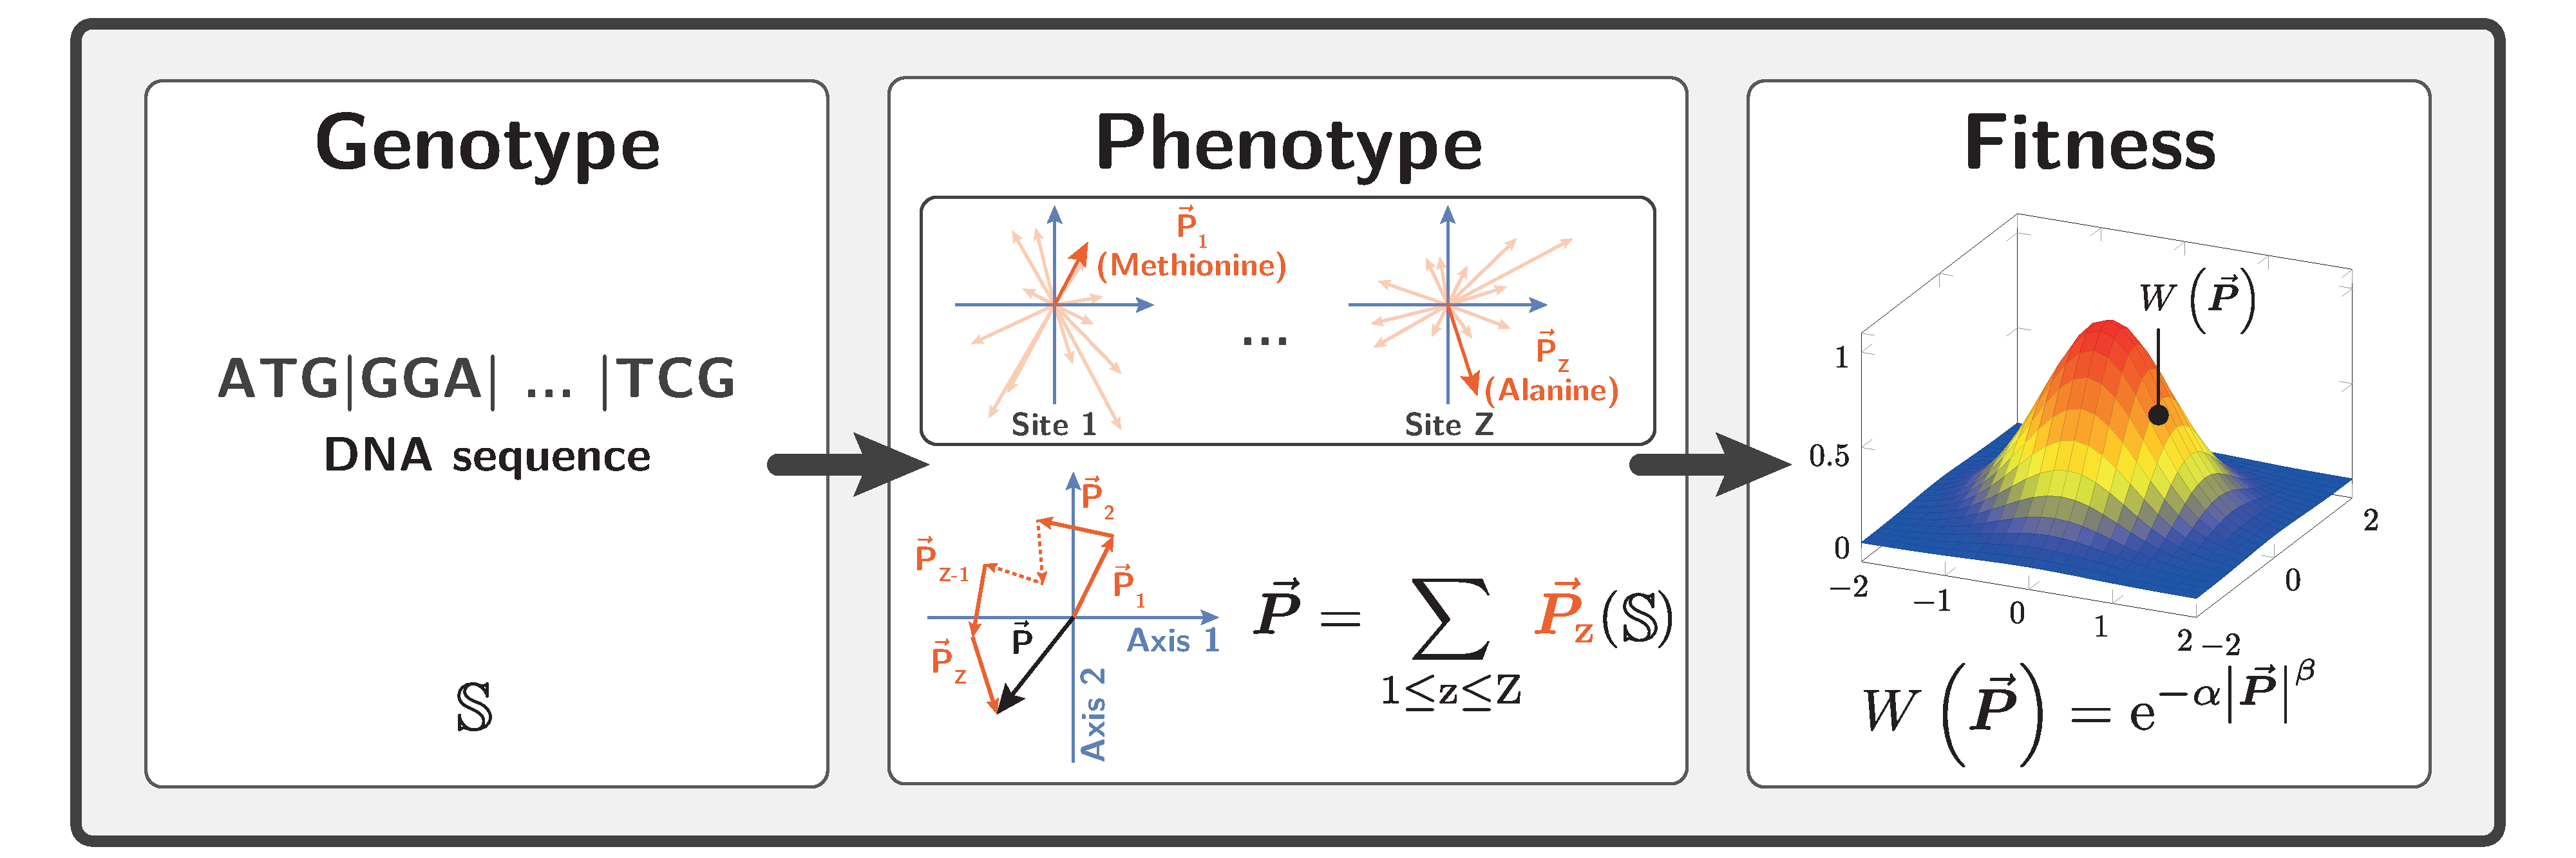
\includegraphics[width=\textwidth] {ModelSimuGeo}
\end{center}
For each possible mutant ($t+1$ substitutions), we compute $\phenoGeo\left(\mathbb{S}^{t+1}\right)$ from the updated sequence $\mathbb{S}^{t+1}$, and subsequently the selection coefficient of the mutant:
\begin{equation}
    s \left( \mathbb{S}^{t},\mathbb{S}^{t+1}\right) = \dfrac{ w\left( \phenoGeo\left(\mathbb{S}^{t+1}\right) \right) - w\left( \phenoGeo\left(\mathbb{S}^{t}\right) \right)}{w\left( \phenoGeo\left(\mathbb{S}^{t}\right) \right)}.
\end{equation}
The next change in the protein coding DNA and the time to next the event is chosen using Gillespie algorithm, according to the rates of substitution between codons:
\begin{equation}
{\submatrix_{\itoj}}
    = \mu_{\itoj} \dfrac{4 \Ne s \left( \mathbb{S}^{t},\mathbb{S}^{t+1}\right)}{{1 - \e^{-4 \Ne s \left( \mathbb{S}^{t},\mathbb{S}^{t+1}\right)} }},
\end{equation}
where ${\submatrix_{\itoj}} = \mu_{\itoj}$ in the case of synonymous substitutions.

\subsection{Protein folding probability}
We simulated substitutions in the protein phosphatase ($\Nsite=300$ codon sites) as in Goldstein \& Pollock (2017).
From a DNA sequence $\mathbb{S}^t$ after $t$ substitutions, we compute the free energy of the folded state $G_{\mathrm{F}}\left(\mathbb{S}^{t}\right)$, using the $3$-dimensional structure of the folded state and pair-wise contact energies between neighboring amino-acid residues:
\begin{equation}
    G_{\mathrm{F}}\left(\mathbb{S}^{t}\right) = \sum_{1 \leq \site \leq \Nsite} \sum_{r \in \mathcal{N}(\site)} I \left(\mathbb{S}^t(\site), \mathbb{S}^t(r) \right),
\end{equation}
where $I(a,b)$ is the pair-wise contact energies between amino-acid $a$ and $b$, using contact potentials estimated by Miya-zawa and Jernigan, and $\mathcal{N}(\site)$ are the neighbor residues of site $\site$ (closer than $7\angstrom$) in the $3$D structure.\\

The free energy of unfolded states $G_{\mathrm{U}}\left(\mathbb{S}^{t}\right)$ is approximated using $55$ decoy $3$D structures that supposedly represent a sample of possible unfolded states:
\begin{equation}
    G_{\mathrm{U}}\left(\mathbb{S}^{t}\right) = \langle G\left(\mathbb{S}^{t}\right) \rangle - kT \ln (1.0\mathrm{E}^{160}) - \dfrac{2 \left[ \langle G\left(\mathbb{S}^{t}\right)^2 \rangle - \langle G\left(\mathbb{S}^{t}\right) \rangle^2\right] }{kT}
\end{equation}
where the average $\langle . \rangle$ runs other the $55$ decoy $3$D structures, and $k$ is the Boltzmann constant and $T$ the temperature in Kelvin.\\

From the energy of folded and unfolded states, we can compute the difference in free energy between the states:
\begin{equation}
    \phenoFold\left(\mathbb{S}^{t}\right) = G_{\mathrm{F}}\left(\mathbb{S}^{t}\right) - G_{\mathrm{U}}\left(\mathbb{S}^{t}\right)
\end{equation}

Wrightian fitness is defined as the probability of our protein to be in the folded state:
\begin{equation}
    w(\phenoFold\left(\mathbb{S}^{t}\right)) = \dfrac{P_{\mathrm{F}}\left(\mathbb{S}^{t}\right)}{P_{\mathrm{F}}\left(\mathbb{S}^{t}\right) + P_{\mathrm{U}}\left(\mathbb{S}^{t}\right)} = \dfrac{e^{-\beta G_{\mathrm{F}}\left(\mathbb{S}^{t}\right) }}{e^{-\beta G_{\mathrm{F}} \left(\mathbb{S}^{t}\right) } + e^{-\beta G_{\mathrm{U}}\left(\mathbb{S}^{t}\right) }} = \dfrac{1}{1 + e^{\beta \phenoFold\left(\mathbb{S}^{t}\right) }},
\end{equation}
where $\beta$ is the inverse of the temperature ($\beta=1/kT$).
\begin{center}
    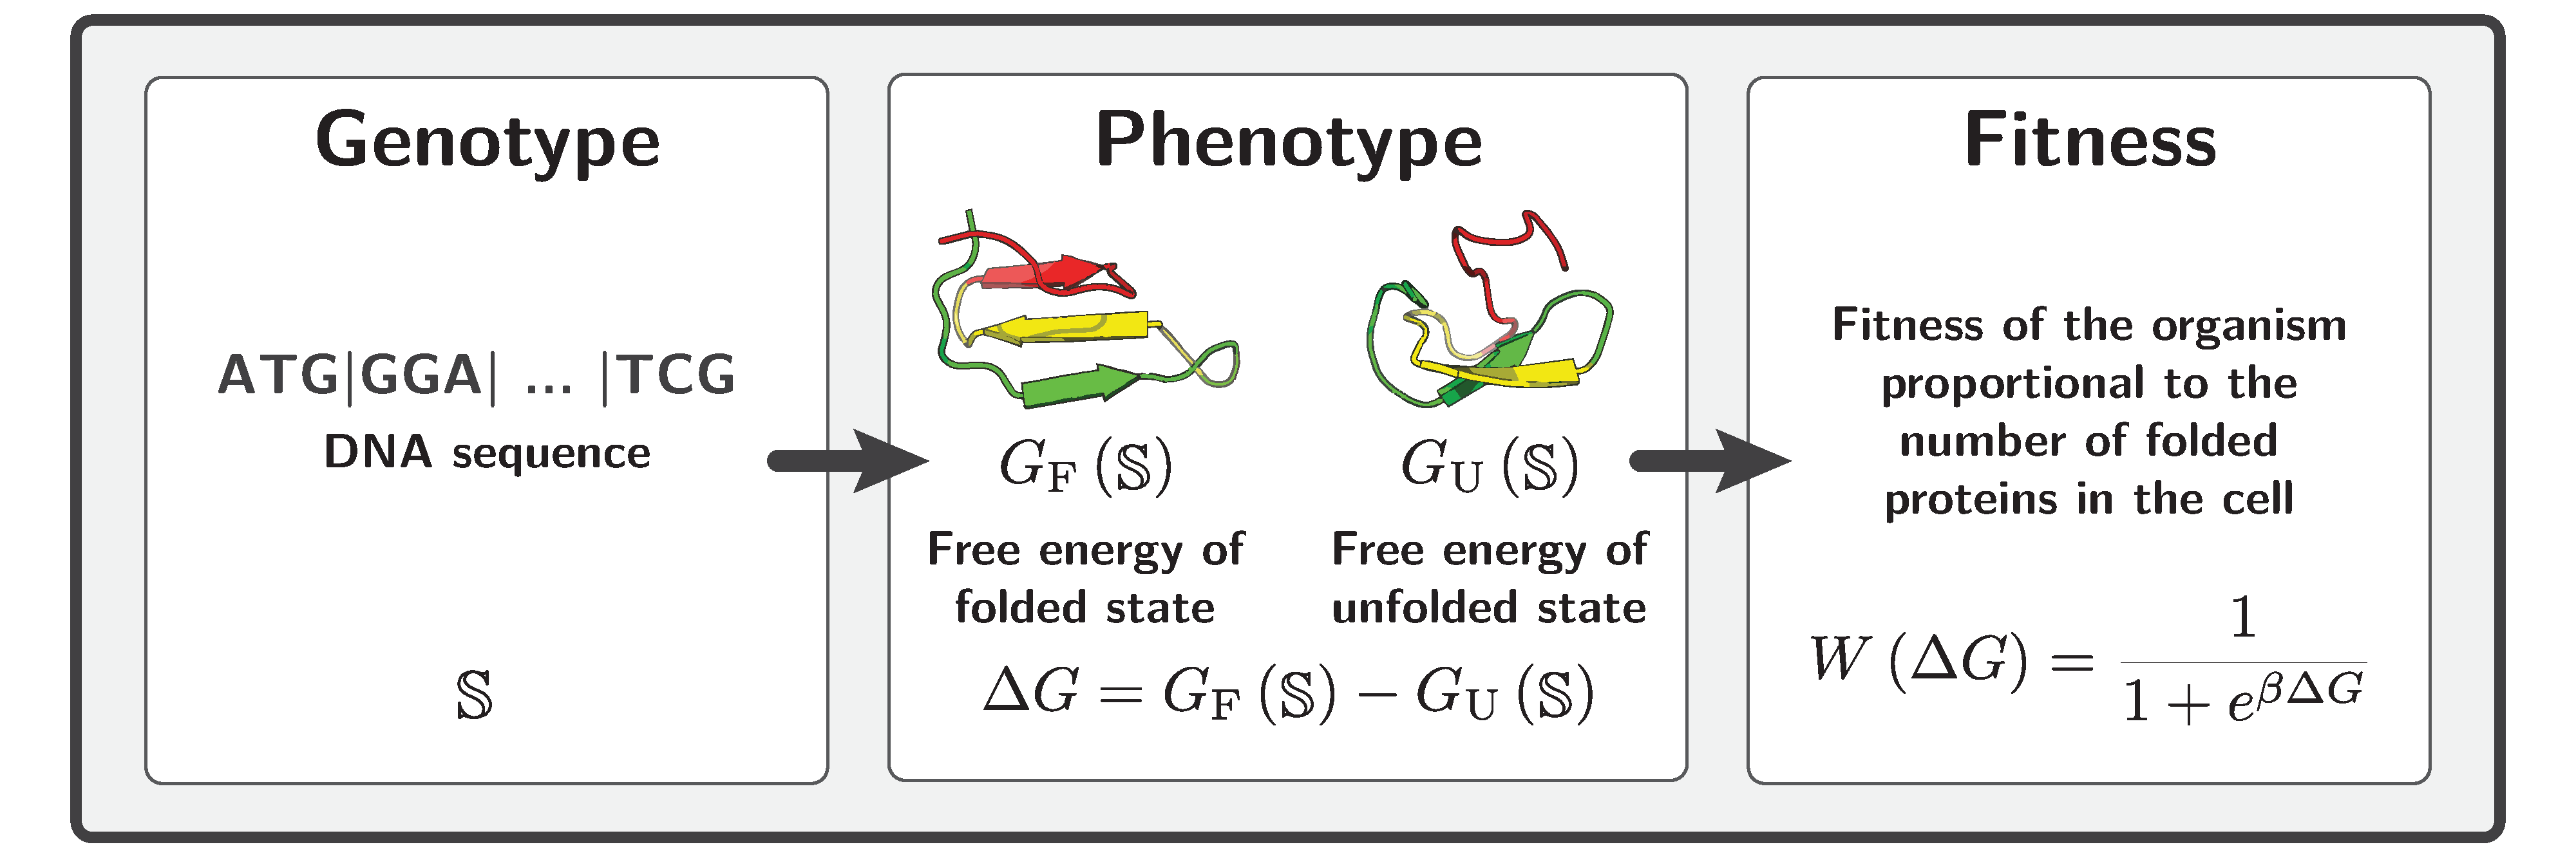
\includegraphics[width=\textwidth] {ModelSimuFold}
\end{center}
For each possible mutant ($t+1$ substitutions), we compute $\phenoFold^{t+1}$ from the updated sequence $\mathbb{S}^{t+1}$, and subsequently the selection coefficient of the mutant:
\begin{equation}
    s \left( \mathbb{S}^{t},\mathbb{S}^{t+1}\right) = \dfrac{ w\left( \phenoFold\left(\mathbb{S}^{t+1}\right) \right) - w\left( \phenoFold\left(\mathbb{S}^{t}\right) \right)}{w\left( \phenoFold\left(\mathbb{S}^{t}\right) \right)}.
\end{equation}
The next change in the protein coding DNA and the time to next the event is chosen using Gillespie algorithm, according to the rates of substitution between codons:
\begin{equation}
{\submatrix_{\itoj}}
    = \mu_{\itoj} \dfrac{4 \Ne s \left( \mathbb{S}^{t},\mathbb{S}^{t+1}\right)}{{1 - \e^{-4 \Ne s \left( \mathbb{S}^{t},\mathbb{S}^{t+1}\right)} }},
\end{equation}
where ${\submatrix_{\itoj}} = \mu_{\itoj}$ in the case of synonymous substitutions.


\section{Simulated experiments}

\subsection{Inferred and simulated branch properties}
Obtained with the inference model of site selection for amino-acid, and branch fluctuation of $\Ne$.

\begin{figure}[H]
    \centering
    \begin{minipage}{0.32\linewidth}
        \includegraphics[width=\linewidth, page=1]{simulations/BranchWise_SimuDiv_SiteMutSelBranchNe_BranchCorrelation_ContrastPopulationSize}
    \end{minipage}    \hfill
    \begin{minipage}{0.32\linewidth}
        \includegraphics[width=\linewidth, page=1]{simulations/SimuPoly_SiteMutSelBranchNe_BranchCorrelation_ContrastPopulationSize}
    \end{minipage}    \hfill
    \begin{minipage}{0.32\linewidth}
        \includegraphics[width=\linewidth, page=1]{simulations/SimuGeo_SiteMutSelBranchNe_BranchCorrelation_ContrastPopulationSize}
    \end{minipage}    \hfill
    \caption[Inferred and simulated $\Ne$ independent contrast]{
    Inferred and simulated $\Ne$ independent contrast.
    Bottom row, independent contrast of $\Ne$ for each branch of the tree, discarding effect of phylogenetic inertia.
    Left panel, simulation accounting for long term fluctuation of $\Ne$, mutation rate per generation and generation time.
    Middle panel, simulation accounting for finite population effects, site linkage and short term fluctuation of $\Ne$.
    Right panel, simulation accounting for site epistasis, thus fluctuation of the selection coefficient along the phylogeny.
    }
\end{figure}

\begin{figure}[H]
    \centering
    \begin{minipage}{0.32\linewidth}
        \includegraphics[width=\linewidth, page=1]{simulations/BranchWise_SimuDiv_SiteMutSelBranchNe_BranchCorrelation_BranchTime}
    \end{minipage}    \hfill
    \begin{minipage}{0.32\linewidth}
        \includegraphics[width=\linewidth, page=1]{simulations/SimuPoly_SiteMutSelBranchNe_BranchCorrelation_BranchTime}
    \end{minipage}    \hfill
    \begin{minipage}{0.32\linewidth}
        \includegraphics[width=\linewidth, page=1]{simulations/SimuGeo_SiteMutSelBranchNe_BranchCorrelation_BranchTime}
    \end{minipage}    \hfill
    \caption[Inferred and simulated branch time]{
    Inferred and simulated branch time ($\Delta T$).
    Left panel, simulation accounting for long term fluctuation of $\Ne$, mutation rate per generation and generation time.
    Middle panel, simulation accounting for finite population effects, site linkage and short term fluctuation of $\Ne$.
    Right panel, simulation accounting for site epistasis, thus fluctuation of the selection coefficient along the phylogeny.
    }
\end{figure}

\begin{figure}[H]
    \centering
    \begin{minipage}{0.32\linewidth}
        \includegraphics[width=\linewidth, page=1]{simulations/BranchWise_SimuDiv_SiteMutSelBranchNe_BranchCorrelation_LogMutationRatePerTime}
    \end{minipage}    \hfill
    \begin{minipage}{0.32\linewidth}
        \includegraphics[width=\linewidth, page=1]{simulations/SimuPoly_SiteMutSelBranchNe_BranchCorrelation_LogMutationRatePerTime}
    \end{minipage}    \hfill
    \begin{minipage}{0.32\linewidth}
        \includegraphics[width=\linewidth, page=1]{simulations/SimuGeo_SiteMutSelBranchNe_BranchCorrelation_LogMutationRatePerTime}
    \end{minipage}    \hfill
    \caption[Inferred and simulated mutation rate]{
    Inferred and simulated mutation rate ($\mu$).
    Left panel, simulation accounting for long term fluctuation of $\Ne$, mutation rate per generation and generation time.
    Middle panel, simulation accounting for finite population effects, site linkage and short term fluctuation of $\Ne$.
    Right panel, simulation accounting for site epistasis, thus fluctuation of the selection coefficient along the phylogeny.
    }
\end{figure}

\subsection{Inferred and simulated site specific amino-acid profiles}

\begin{figure}[H]
    \centering
    \begin{minipage}{0.49\linewidth}
        \includegraphics[width=\linewidth, page=1]{simulations/BranchWise_SimuDiv_SiteMutSelBranchNe_ProfileCorrelation.png}
    \end{minipage}    \hfill
    \begin{minipage}{0.49\linewidth}
        \includegraphics[width=\linewidth, page=1]{simulations/BranchWise_SimuDiv_SiteMutSel_ProfileCorrelation.png}
    \end{minipage}
    \caption[Inferred and simulated amino-acid profiles]{
    Inferred and simulated amino-acid profiles.
    Simulation accounting for long term fluctuation of $\Ne$, mutation rate per generation and generation time.
    Estimation with fluctuating branch $\Ne$ (left panel) or constant $\Ne$ (right panel).}
\end{figure}

\begin{figure}[H]
    \centering
    \begin{minipage}{0.49\linewidth}
        \includegraphics[width=\linewidth, page=1]{simulations/SimuPoly_SiteMutSelBranchNe_ProfileCorrelation.png}
    \end{minipage}    \hfill
    \begin{minipage}{0.49\linewidth}
        \includegraphics[width=\linewidth, page=1]{simulations/SimuPoly_SiteMutSel_ProfileCorrelation.png}
    \end{minipage}
    \caption[Inferred and simulated amino-acid profiles]{Inferred and simulated amino-acid profiles.
    Simulation accounting for finite population effects, site linkage and short term fluctuation of $\Ne$
    Estimation with fluctuating branch $\Ne$ (left panel) or constant $\Ne$ (right panel).}
\end{figure}


\section{Empirical data in mammals}

\subsection{Chain convergence}
Obtained with the inference model of site selection for amino-acid, and branch fluctuation of $\Ne$.

\begin{figure}[H]
    \centering
    \begin{minipage}{0.49\linewidth}
        \includegraphics[width=\linewidth, page=1]{mammals/18CDS_SiteMutSelBranchNe_R1_ProfileCorrelation.png}
    \end{minipage}    \hfill
    \begin{minipage}{0.49\linewidth}
        \includegraphics[width=\linewidth, page=1]{mammals/18CDS_SiteMutSelBranchNe_R1_LogPopulationSizeCorrelation}
    \end{minipage}
    \caption[Chain convergence of site profiles and branche $\Ne$]{
    Chain convergence of site amino-acid preferences (left panel) and branch $\Ne$ (right panel).}
\end{figure}

\subsection{Traits estimation \& correlation (replicate 1, chain 1)}
Obtained with the inference model of site selection for amino-acid, and branch fluctuation of $\Ne$.

\begin{table}[H]
    \centering
\noindent\adjustbox{max width=\textwidth}{%
\begin{tabu}{|c||c|c|c|}
\hline
\textbf{Covariance ($\bm{\Sigma}$)} & $\bm{N_{\mathrm{e}}}$ & $\bm{\mu}$ & \textbf{LogGenomeSize}\\
\hhline{|=#=|=|=|}
$\bm{N_{\mathrm{e}}}$ & $0.506^{**}$ & $-0.112$ & $-0.0231$\\\hline
$\bm{\mu}$ & - & $6.06^{**}$ & $0.129$\\\hline
\textbf{LogGenomeSize} & - & - & $0.0515^{**}$\\\hline
\end{tabu}}

    \caption[Covariance matrix in mammals]{
    Covariance coefficient between effective population size~($\Ne$), mutation rate per site per unit of time~($\mu$), and life-history traits (Maximum longevity, adult weight and female maturity) were computed in placental mammals.
    Asterisks indicate strength of support ($\smash{^{*}} pp > 0.95$, $\smash{^{**}} pp > 0.975$).}
\end{table}

\begin{table}[H]
    \centering
\noindent\adjustbox{max width=\textwidth}{%
\begin{tabu}{|c||c|c|c|c|c|}
\hline
\textbf{Partial coefficient} & $\bm{N_{\mathrm{e}}}$ & $\bm{\mu}$ & \textbf{Maximum longevity } & \textbf{Adult weight } & \textbf{Female maturity }\\
\hhline{|=#=|=|=|=|=|}
$\bm{N_{\mathrm{e}}}$ & - & $-0.146$ & $-0.177$ & $-0.265^{*}$ & $-0.0223$\\\hline
$\bm{\mu}$ & - & - & $-0.283^{*}$ & $-0.396^{**}$ & $-0.327^{**}$\\\hline
\textbf{Maximum longevity } & - & - & - & $0.236^{*}$ & $0.383^{**}$\\\hline
\textbf{Adult weight } & - & - & - & - & $0.179$\\\hline
\textbf{Female maturity } & - & - & - & - & -\\\hline
\end{tabu}}

    \caption[Partial correlation coefficient matrix in mammals]{
    Partial correlation coefficient between effective population size~($\Ne$), mutation rate per site per unit of time~($\mu$), and life-history traits (Maximum longevity, adult weight and female maturity) were computed in placental mammals.
    Asterisks indicate strength of support ($\smash{^{*}} pp > 0.95$, $\smash{^{**}} pp > 0.975$).}
\end{table}

\begin{figure}[H]
    \centering
    \includegraphics[width=\linewidth, page=1]{mammals/18CDS_SiteMutSelBranchNe_R1_LogMaximum_longevity}
    \caption[Maximum longevity estimation in mammals]{Maximum longevity estimation in mammals}
\end{figure}

\begin{figure}[H]
    \centering
    \includegraphics[width=\linewidth, page=1]{mammals/18CDS_SiteMutSelBranchNe_R1_LogAdult_weight}
    \caption[Adult weight estimation in mammals]{Adult weight estimation in mammals}
\end{figure}

\begin{figure}[H]
    \centering
    \includegraphics[width=\linewidth, page=1]{mammals/18CDS_SiteMutSelBranchNe_R1_LogFemale_maturity}
    \caption[Female maturity estimation in mammals]{Female maturity estimation in mammals}
\end{figure}

\subsection{Repeatability of experiments}
Obtained with the inference model of site selection for amino-acid, and branch fluctuation of $\Ne$.

\begin{figure}[H]
    \centering
    \begin{minipage}{0.32\linewidth}
        \includegraphics[width=\linewidth, page=1]{mammals/18CDS_SiteMutSelBranchNe_Rep_LogMutationRatePerTime-1-2}
    \end{minipage}    \hfill
    \begin{minipage}{0.32\linewidth}
        \includegraphics[width=\linewidth, page=1]{mammals/18CDS_SiteMutSelBranchNe_Rep_LogMutationRatePerTime-1-3}
    \end{minipage}    \hfill
    \begin{minipage}{0.32\linewidth}
        \includegraphics[width=\linewidth, page=1]{mammals/18CDS_SiteMutSelBranchNe_Rep_LogMutationRatePerTime-1-4}
    \end{minipage}
    \caption[Repeatability of mutation rate estimation in mammals]{Repeatability of mutation rate ($\mu$) estimation in mammals}
\end{figure}

\begin{figure}[H]
    \centering
    \begin{minipage}{0.32\linewidth}
        \includegraphics[width=\linewidth, page=1]{mammals/18CDS_SiteMutSelBranchNe_Rep_BranchTime-1-2}
    \end{minipage}    \hfill
    \begin{minipage}{0.32\linewidth}
        \includegraphics[width=\linewidth, page=1]{mammals/18CDS_SiteMutSelBranchNe_Rep_BranchTime-1-3}
    \end{minipage}    \hfill
    \begin{minipage}{0.32\linewidth}
        \includegraphics[width=\linewidth, page=1]{mammals/18CDS_SiteMutSelBranchNe_Rep_BranchTime-1-4}
    \end{minipage}
    \caption[Repeatability of branch time estimation in mammals]{Repeatability of branch time ($\Delta T$) estimation in mammals}
\end{figure}

\begin{table}[H]
    \centering
\noindent\adjustbox{max width=\textwidth}{%
\begin{tabu}{|c||c|c|c|c|c|}
\hline
\textbf{Correlation ($\bm{\rho}$)} & $\bm{N_{\mathrm{e}}}$ & $\bm{\mu}$ & \textbf{Maximum longevity } & \textbf{Adult weight } & \textbf{Female maturity }\\
\hhline{|=#=|=|=|=|=|}
$\bm{N_{\mathrm{e}}}$ & - & $0.439^{**}$ & $-0.523^{**}$ & $-0.544^{**}$ & $-0.47^{**}$\\\hline
$\bm{\mu}$ & - & - & $-0.832^{**}$ & $-0.835^{**}$ & $-0.833^{**}$\\\hline
\textbf{Maximum longevity } & - & - & - & $0.827^{**}$ & $0.845^{**}$\\\hline
\textbf{Adult weight } & - & - & - & - & $0.809^{**}$\\\hline
\textbf{Female maturity } & - & - & - & - & -\\\hline
\end{tabu}}
 \\
    \centering
\noindent\adjustbox{max width=\textwidth}{%
\begin{tabu}{|c||c|c|c|}
\hline
\textbf{Correlation ($\bm{\rho}$)} & $\bm{N_{\mathrm{e}}}$ & $\bm{\mu}$ & \textbf{LogGenomeSize}\\
\hhline{|=#=|=|=|}
$\bm{N_{\mathrm{e}}}$ & - & $-0.174$ & $-0.0129$\\\hline
$\bm{\mu}$ & - & - & $0.0964$\\\hline
\textbf{LogGenomeSize} & - & - & -\\\hline
\end{tabu}}
 \\
    \centering
\noindent\adjustbox{max width=\textwidth}{%
\begin{tabu}{|c||c|c|c|c|c|}
\hline
\textbf{Correlation ($\bm{\rho}$)} & $\bm{N_{\mathrm{e}}}$ & $\bm{\mu}$ & \textbf{Maximum longevity } & \textbf{Adult weight } & \textbf{Female maturity }\\
\hhline{|=#=|=|=|=|=|}
$\bm{N_{\mathrm{e}}}$ & - & $0.497^{**}$ & $-0.643^{**}$ & $-0.577^{**}$ & $-0.627^{**}$\\\hline
$\bm{\mu}$ & - & - & $-0.803^{**}$ & $-0.795^{**}$ & $-0.739^{**}$\\\hline
\textbf{Maximum longevity } & - & - & - & $0.836^{**}$ & $0.843^{**}$\\\hline
\textbf{Adult weight } & - & - & - & - & $0.805^{**}$\\\hline
\textbf{Female maturity } & - & - & - & - & -\\\hline
\end{tabu}}
 \\
    \centering
\noindent\adjustbox{max width=\textwidth}{%
\begin{tabu}{|c||c|c|c|}
\hline
\textbf{Correlation ($\bm{\rho}$)} & $\bm{N_{\mathrm{e}}}$ & $\bm{\mu}$ & Genome size\\
\hhline{|=#=|=|=|}
$\bm{N_{\mathrm{e}}}$ & - & $-0.0355$ & $-0.0875$\\\hline
$\bm{\mu}$ & - & - & $0.225$\\\hline
Genome size & - & - & -\\\hline
\end{tabu}}

    \caption[Covariance matrix repeatability in mammals]{
    In all four replicates, covariance coefficient between effective population size~($\Ne$), mutation rate per site per unit of time~($\mu$), and life-history traits (Maximum longevity, adult weight and female maturity) were computed in placental mammals.
    Asterisks indicate strength of support ($\smash{^{*}} pp > 0.95$, $\smash{^{**}} pp > 0.975$).}
\end{table}

\subsection{Amino-acid preferences entropy}

\begin{table}[H]
    \centering
    \noindent\adjustbox{max width=\textwidth}{%
    \begin{tabu}{|c|c|c|}
        \hline
        $\langle \Omega \left( \Fit \right) \rangle$ & \specialcell{\textbf{Constant} $\Ne$} & \specialcell{\textbf{log-Brownian} $\Ne$} \\
        \hline
        \hline\specialcell{Placental mammals, replicate $1$, chain $1$} & $1.34 \pm 0.09$ & $1.24 \pm 0.09$ \\
        \hline\specialcell{Placental mammals, replicate $1$, chain $2$} & $1.33 \pm 0.08$ & $1.27 \pm 0.10$ \\
        \hline\specialcell{Placental mammals, replicate $2$, chain $1$} & $1.40 \pm 0.06$ & $1.31 \pm 0.09$ \\
        \hline\specialcell{Placental mammals, replicate $2$, chain $2$} & $1.42 \pm 0.07$ & $1.28 \pm 0.11$ \\
        \hline\specialcell{Placental mammals, replicate $3$, chain $1$} & $1.23 \pm 0.08$ & $1.25 \pm 0.12$ \\
        \hline\specialcell{Placental mammals, replicate $3$, chain $2$} & $1.25 \pm 0.09$ & $1.24 \pm 0.10$ \\
        \hline
    \end{tabu}}
    \caption[Entropy of amino-acids in mammals]{Entropy of amino-acids}
\end{table}

\subsection{Traits estimation with branch \texorpdfstring{$\omega$}{ω} (replicate 1, chain 1)}
Obtained with the model of branch fluctuation of $\dnds$ (without site selection for amino-acid).

\begin{figure}[H]
    \centering
    \includegraphics[width=\linewidth, page=1]{mammals/18CDS_BranchOmega_R1_LogdNdS}
    \caption[$\dnds$ estimation in mammals]{Non-synonymous substitution rate ($\dnds$) estimation in mammals}
\end{figure}

\begin{table}[H]
    \centering
\noindent\adjustbox{max width=\textwidth}{%
\begin{tabu}{|c||c|c|c|c|c|}
\hline
\textbf{Correlation ($\bm{\rho}$)} & $\bm{\omega}$ & $\bm{\mu}$ & \textbf{Maximum longevity } & \textbf{Adult weight } & \textbf{Female maturity }\\
\hhline{|=#=|=|=|=|=|}
$\bm{\omega}$ & - & $-0.374^{**}$ & $0.544^{**}$ & $0.43^{**}$ & $0.433^{**}$\\\hline
$\bm{\mu}$ & - & - & $-0.807^{**}$ & $-0.781^{**}$ & $-0.824^{**}$\\\hline
\textbf{Maximum longevity } & - & - & - & $0.801^{**}$ & $0.83^{**}$\\\hline
\textbf{Adult weight } & - & - & - & - & $0.785^{**}$\\\hline
\textbf{Female maturity } & - & - & - & - & -\\\hline
\end{tabu}}

    \caption[Correlation coefficient matrix in mammals ($\dnds$)]{
    Correlation coefficient between Non-synonymous substitution rate~($\dnds$), mutation rate per site per unit of time~($\mu$), and life-history traits (Maximum longevity, adult weight and female maturity) were computed in placental mammals.
    Asterisks indicate strength of support ($\smash{^{*}} pp > 0.95$, $\smash{^{**}} pp > 0.975$).}
\end{table}

\begin{table}[H]
    \centering
\noindent\adjustbox{max width=\textwidth}{%
\begin{tabu}{|c||c|c|c|c|c|}
\hline
\textbf{Covariance ($\bm{\Sigma}$)} & $\bm{\omega}$ & $\bm{\mu}$ & \textbf{Maximum longevity } & \textbf{Adult weight } & \textbf{Female maturity }\\
\hhline{|=#=|=|=|=|=|}
$\bm{\omega}$ & $0.215^{**}$ & $-0.236^{**}$ & $0.231^{**}$ & $0.828^{**}$ & $0.242^{**}$\\\hline
$\bm{\mu}$ & - & $1.82^{**}$ & $-0.998^{**}$ & $-4.38^{**}$ & $-1.34^{**}$\\\hline
\textbf{Maximum longevity } & - & - & $0.837^{**}$ & $3.04^{**}$ & $0.917^{**}$\\\hline
\textbf{Adult weight } & - & - & - & $17.1^{**}$ & $3.93^{**}$\\\hline
\textbf{Female maturity } & - & - & - & - & $1.45^{**}$\\\hline
\end{tabu}}

    \caption[Covariance matrix in mammals ($\dnds$)]{
    Correlation coefficient between Non-synonymous substitution rate~($\dnds$), mutation rate per site per unit of time~($\mu$), and life-history traits (Maximum longevity, adult weight and female maturity) were computed in placental mammals.
    Asterisks indicate strength of support ($\smash{^{*}} pp > 0.95$, $\smash{^{**}} pp > 0.975$).}
\end{table}

\begin{table}[H]
    \centering
\noindent\adjustbox{max width=\textwidth}{%
\begin{tabu}{|c||c|c|c|}
\hline
\textbf{Partial coefficient} & $\bm{\omega}$ & $\bm{\mu}$ & \textbf{LogGenomeSize}\\
\hhline{|=#=|=|=|}
$\bm{\omega}$ & - & $0.107$ & $0.121$\\\hline
$\bm{\mu}$ & - & - & $0.235$\\\hline
\textbf{LogGenomeSize} & - & - & -\\\hline
\end{tabu}}

    \caption[Partial correlation coefficient matrix in mammals ($\dnds$)]{
    Partial correlation coefficient between Non-synonymous substitution rate~($\dnds$), mutation rate per site per unit of time~($\mu$), and life-history traits (Maximum longevity, adult weight and female maturity) were computed in placental mammals.
    Asterisks indicate strength of support ($\smash{^{*}} pp > 0.95$, $\smash{^{**}} pp > 0.975$).}
\end{table}


\section{Isopods}

\subsection{Traits estimation (replicate 1, chain 1)}
Obtained with the inference model of site selection for amino-acid, and branch fluctuation of $\Ne$.

\begin{figure}[H]
    \centering
    \includegraphics[width=\linewidth, page=1]{isopods/12CDS_SiteMutSelBranchNe_R1_LogPopulationSize}
    \caption[$\Ne$ estimation in isopods]{Effective population size ($\Ne$) estimation in isopods}
\end{figure}

\begin{figure}[H]
    \centering
    \includegraphics[width=\linewidth, page=1]{isopods/12CDS_SiteMutSelBranchNe_R1_LogMutationRatePerTime}
    \caption[Mutation rate estimation in isopods]{Mutation rate ($\mu$) estimation in isopods}
\end{figure}

\subsection{Repeatability of experiments}
Obtained with the inference model of site selection for amino-acid, and branch fluctuation of $\Ne$.

\begin{figure}[H]
    \centering
    \begin{minipage}{0.32\linewidth}
        \includegraphics[width=\linewidth, page=1]{isopods/12CDS_SiteMutSelBranchNe_Rep-1-2_Log10BranchLength}
    \end{minipage}    \hfill
    \begin{minipage}{0.32\linewidth}
        \includegraphics[width=\linewidth, page=1]{isopods/12CDS_SiteMutSelBranchNe_Rep-1-3_Log10BranchLength}
    \end{minipage}    \hfill
    \begin{minipage}{0.32\linewidth}
        \includegraphics[width=\linewidth, page=1]{isopods/12CDS_SiteMutSelBranchNe_Rep-1-4_Log10BranchLength}
    \end{minipage}
    \begin{minipage}{0.32\linewidth}
        \includegraphics[width=\linewidth, page=1]{isopods/12CDS_SiteMutSelBranchNe_Rep-1-5_Log10BranchLength}
    \end{minipage}
    \begin{minipage}{0.32\linewidth}
        \includegraphics[width=\linewidth, page=1]{isopods/12CDS_SiteMutSelBranchNe_Rep-1-6_Log10BranchLength}
    \end{minipage}
    \caption[Repeatability of branch length estimation in isopods]{Repeatability of branch length ($\branchlength$) estimation in isopods}
\end{figure}

\begin{figure}[H]
    \centering
    \begin{minipage}{0.32\linewidth}
        \includegraphics[width=\linewidth, page=1]{isopods/12CDS_SiteMutSelBranchNe_Rep-1-2_LogPopulationSize}
    \end{minipage}    \hfill
    \begin{minipage}{0.32\linewidth}
        \includegraphics[width=\linewidth, page=1]{isopods/12CDS_SiteMutSelBranchNe_Rep-1-3_LogPopulationSize}
    \end{minipage}    \hfill
    \begin{minipage}{0.32\linewidth}
        \includegraphics[width=\linewidth, page=1]{isopods/12CDS_SiteMutSelBranchNe_Rep-1-4_LogPopulationSize}
    \end{minipage}
    \begin{minipage}{0.32\linewidth}
        \includegraphics[width=\linewidth, page=1]{isopods/12CDS_SiteMutSelBranchNe_Rep-1-5_LogPopulationSize}
    \end{minipage}
    \begin{minipage}{0.32\linewidth}
        \includegraphics[width=\linewidth, page=1]{isopods/12CDS_SiteMutSelBranchNe_Rep-1-6_LogPopulationSize}
    \end{minipage}
    \caption[Repeatability of $\Ne$ estimation in isopods]{Repeatability of effective population size ($\Ne$) estimation in isopods}
\end{figure}

\begin{figure}[H]
    \centering
    \begin{minipage}{0.32\linewidth}
        \includegraphics[width=\linewidth, page=1]{isopods/12CDS_SiteMutSelBranchNe_Rep-1-2_LogMutationRatePerTime}
    \end{minipage}    \hfill
    \begin{minipage}{0.32\linewidth}
        \includegraphics[width=\linewidth, page=1]{isopods/12CDS_SiteMutSelBranchNe_Rep-1-3_LogMutationRatePerTime}
    \end{minipage}    \hfill
    \begin{minipage}{0.32\linewidth}
        \includegraphics[width=\linewidth, page=1]{isopods/12CDS_SiteMutSelBranchNe_Rep-1-4_LogMutationRatePerTime}
    \end{minipage}
    \begin{minipage}{0.32\linewidth}
        \includegraphics[width=\linewidth, page=1]{isopods/12CDS_SiteMutSelBranchNe_Rep-1-5_LogMutationRatePerTime}
    \end{minipage}
    \begin{minipage}{0.32\linewidth}
        \includegraphics[width=\linewidth, page=1]{isopods/12CDS_SiteMutSelBranchNe_Rep-1-6_LogMutationRatePerTime}
    \end{minipage}
    \caption[Repeatability of $\mu$ estimation in isopods]{Repeatability of mutation rate ($\mu$) estimation in isopods}
\end{figure}

\begin{figure}[H]
    \centering
    \begin{minipage}{0.32\linewidth}
        \includegraphics[width=\linewidth, page=1]{isopods/12CDS_SiteMutSelBranchNe_Rep-1-2_BranchTime}
    \end{minipage}    \hfill
    \begin{minipage}{0.32\linewidth}
        \includegraphics[width=\linewidth, page=1]{isopods/12CDS_SiteMutSelBranchNe_Rep-1-3_BranchTime}
    \end{minipage}    \hfill
    \begin{minipage}{0.32\linewidth}
        \includegraphics[width=\linewidth, page=1]{isopods/12CDS_SiteMutSelBranchNe_Rep-1-4_BranchTime}
    \end{minipage}
    \begin{minipage}{0.32\linewidth}
        \includegraphics[width=\linewidth, page=1]{isopods/12CDS_SiteMutSelBranchNe_Rep-1-5_BranchTime}
    \end{minipage}
    \begin{minipage}{0.32\linewidth}
        \includegraphics[width=\linewidth, page=1]{isopods/12CDS_SiteMutSelBranchNe_Rep-1-6_BranchTime}
    \end{minipage}
    \caption[Repeatability of branch time estimation in isopods]{Repeatability of branch time ($\Delta T$) estimation in isopods}
\end{figure}

\subsection{Statistical test}
Obtained with the inference model of site selection for amino-acid, and branch fluctuation of $\Ne$.

\begin{figure}[H]
    \centering
    \includegraphics[width=\linewidth, page=1]{isopods/12CDS_SiteMutSelBranchNe_Rep_LogPopulationSize_eco}
    \caption[$\Ne$ as a function of habitat in isopods]{$\Ne$ as a function of habitat in isopods.}
\end{figure}
\begin{verbatim}
Analysis of Variance Table

Response: PopulationSize
Df Sum Sq Mean Sq F value Pr(>F) 
Habitat 1 2.4899 2.48991 83.2450 < 2.2e-16 ***
Replicate 5 0.6446 0.12892 4.3102 0.0007908 ***
Residuals 389 11.6352 0.02991 
---
Signif. codes: 0 ‘***’ 0.001 ‘**’ 0.01 ‘*’ 0.05 ‘.’ 0.1 ‘ ’ 1
\end{verbatim}
\begin{figure}[H]
    \centering
    \includegraphics[width=\linewidth, page=1]{isopods/12CDS_SiteMutSelBranchNe_Rep_LogPopulationSize_pig}
    \caption[$\Ne$ as a function of pigmentation in isopods]{$\Ne$ as a function of pigmentation in isopods}
\end{figure}
\begin{verbatim}
Analysis of Variance Table

Response: PopulationSize
Df Sum Sq Mean Sq F value Pr(>F) 
Pigmentation 2 2.8413 1.42067 48.850 < 2.2e-16 ***
Replicate 5 0.6446 0.12892 4.433 0.0006135 ***
Residuals 388 11.2838 0.02908 
---
Signif. codes: 0 ‘***’ 0.001 ‘**’ 0.01 ‘*’ 0.05 ‘.’ 0.1 ‘ ’ 1
\end{verbatim}
\begin{figure}[H]
    \centering
    \includegraphics[width=\linewidth, page=1]{isopods/12CDS_SiteMutSelBranchNe_Rep_LogPopulationSize_eye}
    \caption[$\Ne$ as a function of ocular structure in isopods]{$\Ne$ as a function of ocular structure in isopods}
\end{figure}
\begin{verbatim}
Analysis of Variance Table

Response: PopulationSize
Df Sum Sq Mean Sq F value Pr(>F) 
Ocular.structure 2 2.8463 1.42314 48.9571 < 2.2e-16 ***
Replicate 5 0.6446 0.12892 4.4349 0.000611 ***
Residuals 388 11.2789 0.02907 
---
Signif. codes: 0 ‘***’ 0.001 ‘**’ 0.01 ‘*’ 0.05 ‘.’ 0.1 ‘ ’ 1
\end{verbatim}
\begin{figure}[H]
    \centering
    \begin{minipage}{0.32\linewidth}
        \includegraphics[width=\linewidth, page=1]{isopods/12CDS_SiteMutSelBranchNe_Rep_LogPopulationSize_eco_merged}
    \end{minipage}    \hfill
    \begin{minipage}{0.32\linewidth}
        \includegraphics[width=\linewidth, page=1]{isopods/12CDS_SiteMutSelBranchNe_Rep_LogPopulationSize_pig_merged}
    \end{minipage}    \hfill
    \begin{minipage}{0.32\linewidth}
        \includegraphics[width=\linewidth, page=1]{isopods/12CDS_SiteMutSelBranchNe_Rep_LogPopulationSize_eye_merged}
    \end{minipage}
    \caption[$\Ne$ as a function of traits in isopods]{$\Ne$ as a function of traits in isopods}
\end{figure}


\section{Primates}

\subsection{Chain convergence}
Obtained with the inference model of site selection for amino-acid, and branch fluctuation of $\Ne$.

\begin{figure}[H]
    \centering
    \begin{minipage}{0.49\linewidth}
        \includegraphics[width=\linewidth, page=1]{primates/SiteMutSelBranchNe_ProfileCorrelation.png}
    \end{minipage}    \hfill
    \begin{minipage}{0.49\linewidth}
        \includegraphics[width=\linewidth, page=1]{primates/SiteMutSelBranchNe_LogPopulationSizeCorrelation}
    \end{minipage}
    \caption[Chain convergence of site profiles and branche $\Ne$]{
    Chain convergence of site amino-acid preferences (left panel) and branch $\Ne$ (right panel).}
\end{figure}

\subsection{Traits estimation (chain 1)}
Obtained with the inference model of site selection for amino-acid, and branch fluctuation of $\Ne$.

\begin{table}[H]
    \centering
\noindent\adjustbox{max width=\textwidth}{%
\begin{tabu}{|c||c|c|c|c|c|c|c|c|}
\hline
\textbf{Correlation ($\bm{\rho}$)} & $\bm{N_{\mathrm{e}}}$ & $\bm{\mu}$ & \textbf{maturity} & \textbf{mass} & \textbf{longevity} & $\bm{\pi_{S}}$ & $\bm{\pi_{N}/\pi_{S}}$ & \textbf{generation time}\\
\hhline{|=#=|=|=|=|=|=|=|=|}
$\bm{N_{\mathrm{e}}}$ & - & $-0.433^{**}$ & $0.155$ & $0.166$ & $0.157$ & $-0.133$ & $0.104$ & $0.16$\\\hline
$\bm{\mu}$ & - & - & $-0.792^{**}$ & $-0.791^{**}$ & $-0.773^{**}$ & $0.62^{**}$ & $-0.59$ & $-0.78^{**}$\\\hline
\textbf{maturity} & - & - & - & $0.986^{**}$ & $0.985^{**}$ & $-0.8^{**}$ & $0.746$ & $0.991^{**}$\\\hline
\textbf{mass} & - & - & - & - & $0.977^{**}$ & $-0.737^{**}$ & $0.695$ & $0.981^{**}$\\\hline
\textbf{longevity} & - & - & - & - & - & $-0.819^{**}$ & $0.752$ & $0.999^{**}$\\\hline
$\bm{\pi_{S}}$ & - & - & - & - & - & - & $-0.86^{**}$ & $-0.816^{**}$\\\hline
$\bm{\pi_{N}/\pi_{S}}$ & - & - & - & - & - & - & - & $0.752$\\\hline
\textbf{generation time} & - & - & - & - & - & - & - & -\\\hline
\end{tabu}}

    \caption[Correlation coefficient matrix in primates ($\Ne$)]{
    Correlation coefficient between effective population size~($\Ne$), mutation rate per site per unit of time~($\mu$), and life-history traits (Maximum longevity, adult weight and female maturity) were computed in placental mammals.
    Asterisks indicate strength of support ($\smash{^{*}} pp > 0.95$, $\smash{^{**}} pp > 0.975$).}
\end{table}

\begin{table}[H]
    \centering
\noindent\adjustbox{max width=\textwidth}{%
\begin{tabu}{|c||c|c|c|c|c|c|c|c|}
\hline
\textbf{Covariance ($\bm{\Sigma}$)} & $\bm{N_{\text{e}}}$ & $\bm{\mu}$ & \textbf{maturity} & \textbf{mass} & \textbf{longevity} & $\bm{\pi_{S}}$ & $\bm{\pi_{N}/\pi_{S}}$ & \textbf{generation time}\\
\hhline{|=#=|=|=|=|=|=|=|=|}
$\bm{N_{\text{e}}}$ & $1.08^{**}$ & $-1.39^{**}$ & $0.66$ & $1.18$ & $0.414$ & $-0.251$ & $0.0898$ & $0.452$\\\hline
$\bm{\mu}$ & - & $9.86^{**}$ & $-10.1^{**}$ & $-17.5^{**}$ & $-6.44^{**}$ & $3.42^{**}$ & $-1.28$ & $-6.96^{**}$\\\hline
\textbf{maturity} & - & - & $16.9^{**}$ & $28.4^{**}$ & $10.6^{**}$ & $-5.39^{**}$ & $1.9$ & $11.5^{**}$\\\hline
\textbf{mass} & - & - & - & $49.8^{**}$ & $18.1^{**}$ & $-8.89^{**}$ & $3.29$ & $19.5^{**}$\\\hline
\textbf{longevity} & - & - & - & - & $6.99^{**}$ & $-3.75^{**}$ & $1.31$ & $7.47^{**}$\\\hline
$\bm{\pi_{S}}$ & - & - & - & - & - & $3.26^{**}$ & $-0.986^{**}$ & $-3.96^{**}$\\\hline
$\bm{\pi_{N}/\pi_{S}}$ & - & - & - & - & - & - & $0.419^{**}$ & $1.39$\\\hline
\textbf{generation time} & - & - & - & - & - & - & - & $8.02^{**}$\\\hline
\end{tabu}}

    \caption[Covariance matrix in primates ($\Ne$)]{
    Correlation coefficient between effective population size~($\Ne$), mutation rate per site per unit of time~($\mu$), and life-history traits (Maximum longevity, adult weight and female maturity) were computed in placental mammals.
    Asterisks indicate strength of support ($\smash{^{*}} pp > 0.95$, $\smash{^{**}} pp > 0.975$).}
\end{table}

\begin{table}[H]
    \centering
\noindent\adjustbox{max width=\textwidth}{%
\begin{tabu}{|c||c|c|c|c|c|c|c|c|}
\hline
\textbf{Partial coefficient} & $\bm{N_{\text{e}}}$ & $\bm{\mu}$ & \textbf{maturity} & \textbf{mass} & \textbf{longevity} & $\bm{\pi_{S}}$ & $\bm{\pi_{N}/\pi_{S}}$ & \textbf{generation time}\\
\hhline{|=#=|=|=|=|=|=|=|=|}
$\bm{N_{\text{e}}}$ & - & $-0.411$ & $-0.0622$ & $0.0184$ & $-0.0436$ & $-0.0482$ & $-0.00476$ & $0.0333$\\\hline
$\bm{\mu}$ & - & - & $0.0548$ & $-0.101$ & $0.146$ & $-0.0134$ & $-0.102$ & $-0.124$\\\hline
\textbf{maturity} & - & - & - & $0.292$ & $-0.793^{**}$ & $-0.167$ & $0.0547$ & $0.824^{**}$\\\hline
\textbf{mass} & - & - & - & - & $-0.0589$ & $0.43$ & $-0.195$ & $0.101$\\\hline
\textbf{longevity} & - & - & - & - & - & $-0.159$ & $-0.148$ & $0.991^{**}$\\\hline
$\bm{\pi_{S}}$ & - & - & - & - & - & - & $-0.573^{**}$ & $0.11$\\\hline
$\bm{\pi_{N}/\pi_{S}}$ & - & - & - & - & - & - & - & $0.144$\\\hline
\textbf{generation time} & - & - & - & - & - & - & - & -\\\hline
\end{tabu}}

    \caption[Partial correlation coefficient matrix in primates ($\Ne$)]{
    Partial correlation coefficient between Neffective population size~($\Ne$), mutation rate per site per unit of time~($\mu$), and life-history traits (Maximum longevity, adult weight and female maturity) were computed in placental mammals.
    Asterisks indicate strength of support ($\smash{^{*}} pp > 0.95$, $\smash{^{**}} pp > 0.975$).}
\end{table}

\begin{figure}[H]
    \centering
    \includegraphics[width=\linewidth, page=1]{primates/SiteMutSelBranchNe_LogPopulationSize}
    \caption[$\Ne$ estimation in primates]{Effective population size ($\Ne$) estimation in primates}
\end{figure}

\begin{figure}[H]
    \centering
    \includegraphics[width=\linewidth, page=1]{primates/SiteMutSelBranchNe_LogMutationRatePerTime}
    \caption[Mutation rate estimation in primates]{Mutation rate ($\mu$) estimation in primates}
\end{figure}

\begin{figure}[H]
    \centering
    \includegraphics[width=\linewidth, page=1]{primates/SiteMutSelBranchNe_Logmaturity}
    \caption[Female maturity estimation in primates]{Female maturity estimation in primates}
\end{figure}

\begin{figure}[H]
    \centering
    \includegraphics[width=\linewidth, page=1]{primates/SiteMutSelBranchNe_Logmass}
    \caption[Mass estimation in primates]{Mass estimation in primates}
\end{figure}

\begin{figure}[H]
    \centering
    \includegraphics[width=\linewidth, page=1]{primates/SiteMutSelBranchNe_Loglongevity}
    \caption[Longevity estimation in primates]{Longevity estimation in primates}
\end{figure}

\begin{figure}[H]
    \centering
    \includegraphics[width=\linewidth, page=1]{primates/SiteMutSelBranchNe_LogpiS}
    \caption[$\pi_{S}$ estimation in primates]{$\pi_{S}$ estimation in primates}
\end{figure}

\begin{figure}[H]
    \centering
    \includegraphics[width=\linewidth, page=1]{primates/SiteMutSelBranchNe_LogpiNpiS}
    \caption[$\pi_{N} / \pi_{S}$ estimation in primates]{$\pi_{N} / \pi_{S}$ estimation in primates}
\end{figure}

\begin{figure}[H]
    \centering
    \includegraphics[width=\linewidth, page=1]{primates/SiteMutSelBranchNe_Loggeneration_time}
    \caption[Generation time estimation in primates]{Generation time estimation in primates}
\end{figure}

\subsection{Traits estimation with branch \texorpdfstring{$\omega$}{ω} (chain 1)}
Obtained with the model of branch fluctuation of $\dnds$ (without site selection for amino-acid).

\begin{figure}[H]
    \centering
    \includegraphics[width=\linewidth, page=1]{primates/BranchOmega_LogOmega}
    \caption[$\dnds$ estimation in primates]{Non-synonymous substitution rate ($\dnds$) estimation in primates}
\end{figure}

\begin{figure}[H]
    \centering
    \includegraphics[width=\linewidth, page=1]{primates/BranchOmega_LogMutationRatePerTime}
    \caption[$\mu$ estimation in primates]{Mutation rate ($\mu$) estimation in primates}
\end{figure}

\begin{table}[H]
    \centering
\noindent\adjustbox{max width=\textwidth}{%
\begin{tabu}{|c||c|c|c|c|c|c|c|c|}
\hline
\textbf{Correlation ($\bm{\rho}$)} & $\bm{\omega}$ & $\bm{\mu}$ & \textbf{maturity} & \textbf{mass} & \textbf{longevity} & $\bm{\pi_{S}}$ & $\bm{\pi_{N}/\pi_{S}}$ & \textbf{generation time}\\
\hhline{|=#=|=|=|=|=|=|=|=|}
$\bm{\omega}$ & - & $0.294$ & $0.000316$ & $0.0361$ & $0.0155$ & $-0.197$ & $0.145$ & $0.0111$\\\hline
$\bm{\mu}$ & - & - & $-0.804^{**}$ & $-0.798^{**}$ & $-0.817^{**}$ & $-0.0201$ & $0.031$ & $-0.823^{**}$\\\hline
\textbf{maturity} & - & - & - & $0.952^{**}$ & $0.957^{**}$ & $-0.166$ & $0.162$ & $0.97^{**}$\\\hline
\textbf{mass} & - & - & - & - & $0.933^{**}$ & $-0.0437$ & $0.0427$ & $0.943^{**}$\\\hline
\textbf{longevity} & - & - & - & - & - & $-0.223$ & $0.165$ & $0.999^{**}$\\\hline
$\bm{\pi_{S}}$ & - & - & - & - & - & - & $-0.664$ & $-0.212$\\\hline
$\bm{\pi_{N}/\pi_{S}}$ & - & - & - & - & - & - & - & $0.162$\\\hline
\textbf{generation time} & - & - & - & - & - & - & - & -\\\hline
\end{tabu}}

    \caption[Correlation coefficient matrix in primates ($\dnds$)]{
    Correlation coefficient between Non-synonymous substitution rate~($\dnds$), mutation rate per site per unit of time~($\mu$), and life-history traits (Maximum longevity, adult weight and female maturity) were computed in placental mammals.
    Asterisks indicate strength of support ($\smash{^{*}} pp > 0.95$, $\smash{^{**}} pp > 0.975$).}
\end{table}

\begin{table}[H]
    \centering
\noindent\adjustbox{max width=\textwidth}{%
\begin{tabu}{|c||c|c|c|c|c|c|c|c|}
\hline
\textbf{Covariance ($\bm{\Sigma}$)} & $\bm{\omega}$ & $\bm{\mu}$ & \textbf{maturity} & \textbf{mass} & \textbf{longevity} & $\bm{\pi_{S}}$ & $\bm{\pi_{N}/\pi_{S}}$ & \textbf{generation time}\\
\hhline{|=#=|=|=|=|=|=|=|=|}
$\bm{\omega}$ & $0.0674^{**}$ & $0.231$ & $-0.0106$ & $0.0149$ & $-0.00138$ & $-0.0435$ & $0.0101$ & $-0.00314$\\\hline
$\bm{\mu}$ & - & $8.71^{**}$ & $-4.8^{**}$ & $-9.22^{**}$ & $-3.97^{**}$ & $0.188$ & $0.0483$ & $-4.08^{**}$\\\hline
\textbf{maturity} & - & - & $4.95^{**}$ & $8.37^{**}$ & $3.29^{**}$ & $-1.01$ & $0.000924$ & $3.53^{**}$\\\hline
\textbf{mass} & - & - & - & $16.3^{**}$ & $6.14^{**}$ & $-0.932$ & $-0.0741$ & $6.45^{**}$\\\hline
\textbf{longevity} & - & - & - & - & $2.76^{**}$ & $-0.577$ & $0.0919$ & $2.82^{**}$\\\hline
$\bm{\pi_{S}}$ & - & - & - & - & - & $1.3^{**}$ & $-0.148$ & $-0.637$\\\hline
$\bm{\pi_{N}/\pi_{S}}$ & - & - & - & - & - & - & $0.182^{**}$ & $0.0775$\\\hline
\textbf{generation time} & - & - & - & - & - & - & - & $2.92^{**}$\\\hline
\end{tabu}}

    \caption[Covariance matrix in primates ($\dnds$)]{
    Correlation coefficient between Non-synonymous substitution rate~($\dnds$), mutation rate per site per unit of time~($\mu$), and life-history traits (Maximum longevity, adult weight and female maturity) were computed in placental mammals.
    Asterisks indicate strength of support ($\smash{^{*}} pp > 0.95$, $\smash{^{**}} pp > 0.975$).}
\end{table}

\begin{table}[H]
    \centering
\noindent\adjustbox{max width=\textwidth}{%
\begin{tabu}{|c||c|c|c|c|c|c|c|c|}
\hline
\textbf{Partial coefficient} & $\bm{\omega}$ & $\bm{\mu}$ & \textbf{maturity} & \textbf{mass} & \textbf{longevity} & $\bm{\pi_{S}}$ & $\bm{\pi_{N}/\pi_{S}}$ & \textbf{generation time}\\
\hhline{|=#=|=|=|=|=|=|=|=|}
$\bm{\omega}$ & - & $0.463$ & $-0.0461$ & $0.248$ & $-0.027$ & $-0.193$ & $-0.0681$ & $0.0319$\\\hline
$\bm{\mu}$ & - & - & $0.0649$ & $-0.000258$ & $0.0374$ & $-0.128$ & $0.115$ & $-0.075$\\\hline
\textbf{maturity} & - & - & - & $0.228$ & $-0.834^{**}$ & $-0.0991$ & $0.0491$ & $0.854^{**}$\\\hline
\textbf{mass} & - & - & - & - & $-0.038$ & $0.435$ & $-0.123$ & $0.0851$\\\hline
\textbf{longevity} & - & - & - & - & - & $-0.184$ & $-0.145$ & $0.994^{**}$\\\hline
$\bm{\pi_{S}}$ & - & - & - & - & - & - & $-0.553^{*}$ & $0.125$\\\hline
$\bm{\pi_{N}/\pi_{S}}$ & - & - & - & - & - & - & - & $0.136$\\\hline
\textbf{generation time} & - & - & - & - & - & - & - & -\\\hline
\end{tabu}}

    \caption[Partial correlation coefficient matrix in primates ($\dnds$)]{
    Partial correlation coefficient between Non-synonymous substitution rate~($\dnds$), mutation rate per site per unit of time~($\mu$), and life-history traits (Maximum longevity, adult weight and female maturity) were computed in placental mammals.
    Asterisks indicate strength of support ($\smash{^{*}} pp > 0.95$, $\smash{^{**}} pp > 0.975$).}
\end{table}


\section{Sufficient statistics}

A sequence of length $\Nsite$ evolves by point substitutions, according to a random process defined by the substitution matrices $\Submatrix\branchsiteexp$, over a phylogenetic tree.
A realization of the random process along a branch $\branch$, and at a particular site $\site$ results in a detailed substitution history, which will be denoted by $\subhistory\branchsiteexp$.

\subsubsection{Path sufficient statistics}
All sites owning to the same category of fitness profile share the same substitution rate matrix.
Hence, $\subhistory\branchsiteexp$ can be gathered across all sites owing to a specific category $\cat$, denoted $\subhistory\branchexp$.
If we express the probability of the substitution mapping ($\subhistory\branchcatexp$) as a function of the codon substitution process for this category $\cat$, we get the following expression:
\begin{equation}
    \label{eq:PathSuffStat}
    p(\subhistory\branchcatexp | \branchlength\branchexp, \Submatrix\branchcatexp) \propto \prod_{\iSetCodon} \left[\subequi_{\ci}\branchcatexp\right]^{n_{\ci}\branchcatexp} \prod_{ \ijSetCodon} \left[\submatrix\branchcatexp_{\itoj}\right]^{m_{\ci, \cj}\branchcatexp} \prod_{\iSetCodon} \e^{- \left| \submatrix\branchcatexp_{\ci, \ci}\right| a_{\ci}\branchcatexp}
\end{equation}
where we define the sufficient statistics:
\begin{itemize}
    \setlength\itemsep{-0.25em}
    \item $m_{\ci, \cj}\branchcatexp$ is the total number of substitutions from codon $\ci$ to codon $\cj$
    \item $n_{\ci}\branchcatexp$ is the number of sites starting with codon $\ci$ at the tip of the branch.
    \item $a_{\ci}\branchcatexp$ is the total waiting time in codon $\ci$.
\end{itemize}
Once these sufficient statistics have been computed, the parameters of the substitution matrix $\Submatrix\branchcatexp$ can be resampled conditional on $\subhistory\branchcatexp$,
using equation~\ref{eq:PathSuffStat} each time the likelihood needs to be recomputed. This leads to relatively fast MCMC strategy.

\subsubsection{Length sufficient statistics}
$\subhistory\branchsiteexp$ can also be gathered across all sites along a specific branch, giving $\subhistory\branchexp$.
Then the probability of the substitution history given the branch lengths ($\branchlength\branchexp = \mu\branchexp \branchtime\branchexp$), take a very simple form:
\begin{equation}
    \label{eq:LengthSuffStat}
    p(\subhistory\branchexp | L\branchexp) \propto \left[ L\branchexp\right]^{u\branchexp} \e^{- r\branchexp L\branchexp}
\end{equation}
where we define the sufficient statistics:
\begin{itemize}
    \setlength\itemsep{-0.25em}
    \item $u\branchexp$ is the total number of substitutions over branch $\branch$, summed over all sites.
    \item $r\branchexp$ is the mean rate away from current codon state (averaged over the entire substitution history).
\end{itemize}
Thus, formally, the probability of the substitution mapping can be summarized by saying that the total number of substitutions along a given branch over all sites, $u\branchexp$, is Poisson distributed, of mean $r\branchexp L\branchexp$.

\subsubsection{Scatter sufficient statistics}
From the independent contrast $\contrast\branchexp$ of the Brownian process $\Brownian\nodeexp$, we can define the $2 \times 2$ scatter sufficient statistic matrix, $\Scattermatrix$ as:
\begin{equation}
    \Scattermatrix = \sum_{b=1}^{\Nbranch} \contrast\branchexp \cdot \left[\contrast\branchexp\right]^{\mathrm{T}}
\end{equation}
By Bayes theorem, the posterior on $\Sigma$, conditional on a particular realization of $\brownian$ (and thus of $\contrast$) is an invert Wishart distribution, of parameter $\covariancekappa \Identitymatrix + \Scattermatrix$ and with $\Nbranch + 3$ degrees of freedom.
\begin{equation}
    \CovarianceMatrix \sim \mathrm{Wishart}^{-1}\left( \covariancekappa \Identitymatrix + \Scattermatrix, \Nbranch + 3\right)
\end{equation}
This invert Wishart distribution can be obtained by sampling $\Nbranch + 3$ independent and identically distributed multivariate normal random variables $\Multivariate\indiceexp$ defined by
\begin{equation}
    \Multivariate\indiceexp \sim \mathcal{N} \left( \bm{0}, \left[\covariancekappa \Identitymatrix + \Scattermatrix\right]^{-1} \right).
\end{equation}
And from these multivariate samples, $\CovarianceMatrix$ is Gibbs sampled as:
\begin{equation}
    \CovarianceMatrix = \left( \sum_{k=1}^{\Nbranch + 3} \Multivariate\indiceexp \cdot \left[\Multivariate\indiceexp \right] ^{\mathrm{T}} \right)^{-1}
\end{equation}


\thispagestyle{empty}
\chapter{Substitution rate susceptibility - Supplementary Materials}
{\hypersetup{linkcolor=GREYDARK}\minitoc}
\label{chap:GenoPhenoFit-SuppMat}
\section{\texorpdfstring{$\omega$}{ω} susceptibility after a change in \texorpdfstring{$\Ne$}{Nₑ}}
\subsection{Genotype to phenotype map}
Define $\Nsite$ as the number of sites in the genotype sequence.
Each site can be in one of $\Nstate \geq 2$ states, where only $1$ state is defined the stable state, and $\Nstate - 1$ states are unstable.
For a given genotype sequence, define phenotype $0 \leq x \leq 1$ as the current proportion of sites in the unstable state.
After a mutation, given that only one site can change at a time, the absolute change of $x$ is either $0$ or $\dx=\sfrac{1}{\Nsite}$.
Define $\rho_{x}(\dx)$ as the probability to get a change of phenotype equal to $\dx$, if the current phenotype is $x$:\\
\begin{gather}
\begin{cases}
\dx &\text{ with probability } \rho_{x}(\dx) = 1-x, \\
0 &\text{ with probability } \rho_{x}(0) = x \left[1 - \frac{1}{\Nstate - 1}\right], \\
-\dx &\text{ with probability } \rho_{x}(-\dx) = \frac{x}{\Nstate - 1}.\\
\end{cases} \label{eq:proba-pheno}
\end{gather}
\subsection{Selection coefficient}
$s(x, \dx)$ is the selection coefficient of an effect $\dx$ if the current phenotype is $x$:
\begin{align}
s(x, \dx) &= \frac{f(x + \dx) - f(x)}{f( x)}, \\
 &\simeq \frac{1}{f(x)}\frac{ \partial f(x) }{\partial x} \dx, \\
 &\simeq \frac{ \partial \ln f(x) }{\partial x} \dx, \label{eq:s_from_fitness}
\end{align}
where $f( x)$ is the Wrightian fitness of phenotype $x$. And thus we also have:
\begin{gather}
s(x, -\dx) \simeq - s(x, \dx) \text{ from eq. \ref{eq:s_from_fitness}} \label{eq:s_minus_deltax}, \\
\iff S(x, -\dx) \simeq - S(x, \dx), \label{eq:S_minus_deltax}
\end{gather}
where $S(x\eq, \dx) = 4\Ne s (x\eq, \dx)$ is the scaled selection coefficient.
\subsection{Probability of fixation}
The probability of fixation of a mutation with effect $\dx$, for a resident phenotype $x$ is :
\begin{align}
p_{\text{fix}}(x, \dx) &= \frac{ 1 - \e^{-2 s(x, \dx)}}{1 - \e^{-4\Ne s(x, \dx)}}, \\
 &\simeq \frac{ 2 s(x, \dx)}{1 - \e^{-4\Ne s(x, \dx)}}, \\
 &= \frac{ 2 s(x, \dx)}{1 - \e^{-S(x, \dx)}}. \label{eq:pfix}
\end{align}
And in the case of neutral mutations, the probability of fixation is:
\begin{gather}
p_{\text{fix}}(x, 0) = \frac{ 1}{2 \Ne} \label{eq:pfix0}.
\end{gather}
And the ratio of probability of fixation between selected and neutral mutations is:
\begin{align}
\frac{p_{\text{fix}}(x, \dx)}{p_{\text{fix}}(x, 0)} & = \frac{ 2 \Ne 2 s(x, \dx)}{1 - \e^{-S(x, \dx)}} \text{ from eq. \ref{eq:pfix} and \ref{eq:pfix0}},\\
& = \frac{S(x, \dx)}{1 - \e^{-S(x, \dx)}} \label{eq:pfixratio}.
\end{align}
\subsection{Equilibrium phenotype}
At equilibrium phenotype $x\eq$, the expected selection coefficient of mutation that reached fixation must be $0$:
\begin{gather}
 0 = \E_{\dx} \left[ s(x\eq, \dx) p_{\text{fix}}(x\eq, \dx) \right], \\
\iff 0 = \frac{ 2 s(x\eq, \dx)^2}{1 - \e^{-S(x\eq, \dx)}}   \rho_{x\eq}(\dx) + s(x\eq, 0) \frac{ \rho_{x\eq}(0)}{2\Ne} + \frac{ 2s(x\eq, -\dx)^2}{1 - \e^{-S(x\eq, -\dx)}} \rho_{x\eq}(-\dx)\text{ from eq. \ref{eq:pfix} and \ref{eq:pfix0}}, \\
\Longrightarrow \frac{ 2s(x\eq, \dx)^2}{1 - \e^{-S(x\eq, \dx)}}   \rho_{x\eq}(\dx) \simeq \frac{ - 2s(x\eq, \dx)^2}{1 - \e^{S(x\eq, \dx)}}   \rho_{x\eq}(-\dx) \text{ from eq. \ref{eq:S_minus_deltax}}, \\
\iff \frac{ \rho_{x\eq}(\dx)}{\rho_{x\eq}(-\dx)} \simeq \e^{-S(x\eq, \dx)} \frac{ \e^{-S(x\eq, \dx)} - 1}{ \e^{-S(x\eq, \dx)} \left( 1 - \e^{S(x\eq, \dx)} \right)}, \\
\iff \ln \left( \frac{1 - x\eq}{x\eq} \right) + \ln (\Nstate-1) \simeq -S(x\eq, \dx) \text{ from eq. \ref{eq:proba-pheno}} \label{eq:equilibrium-pheno}, \\
\iff \lambda_{K}(x\eq) \simeq -S(x\eq, \dx) \label{eq:equilibrium_lambda},
\end{gather}
where  $\lambda_{K}(x\eq) = \ln \left( \frac{1 - x\eq}{x\eq} \right) + \ln (\Nstate-1)$.
\subsection{Substitution rate bias (\texorpdfstring{$\omega$}{ω}) at equilibrium}
The substitution rate of selected mutations relative to neutral mutations ($\omega$) is by definition:
\begin{align}
\omega & = \E_{\dx} \left[ \frac{p_{\text{fix}}(x, \dx)}{p_{\text{fix}}(x, 0)} \right], \\
 & = (1 - x) \frac{ S(x, \dx)}{1 - \e^{-S(x, \dx)}} + x \left(\frac{\Nstate - 2}{\Nstate - 1}\right) + \frac{x}{\Nstate-1} \frac{ S(x, -\dx)}{1 - \e^{-S(x, -\dx)}} \text{ from eq. \ref{eq:proba-pheno}, \ref{eq:pfix} and \ref{eq:pfix0}}, \\
 & = (1 - x) \frac{ S(x, \dx)}{1 - \e^{-S(x, \dx)}} - \frac{x}{\Nstate-1}  \frac{ S(x, \dx)}{1 - \e^{S(x, \dx)}} +  x \left(\frac{\Nstate - 2}{\Nstate - 1}\right) \text{ from eq. \ref{eq:S_minus_deltax}}.
\end{align}
$\omega\eq$ at equilibrium is then determined by the phenotype at equilibrium $x\eq$:
\begin{align}
\omega\eq &= (1 - x\eq) \frac{ S(x\eq, \dx)}{1 - \e^{-S(x\eq, \dx)}} - \frac{x\eq}{\Nstate-1} \frac{ S(x\eq, \dx)}{1 - \e^{S(x\eq, \dx)}} + x\eq \left(\frac{\Nstate - 2}{\Nstate - 1}\right) , \\
 &= x\eq \left[ \frac{2 (x\eq-1)  \lambda_{K}(x\eq) }{\Nstate (x\eq-1)+1} + \frac{\Nstate - 2}{\Nstate - 1}\right] \text{ from eq. \ref{eq:equilibrium-pheno}}.
\end{align}
\begin{center}
 \includegraphics[width=0.8\textwidth, page=2] {analytical-relaxation}
\end{center}
Moreover, given that the number of state if large enough $\Nstate \gg 1$, the equilibrium $\omega$ can be approximated as:
\begin{align}
\omega\eq  & = x\eq \left[ \frac{2 (x\eq-1)  \lambda_{K}(x\eq) }{\Nstate (x\eq-1)+1} + \frac{\Nstate - 2}{\Nstate - 1}\right], \\
& \simeq x\eq
\end{align}
And the derivative of $\omega\eq$ w.r.t to $x\eq$ is: 
\begin{gather}
\frac{\der \omega\eq}{\der x\eq} = 2 \left[ \frac{\Nstate (x\eq- 1) + 1+\left[\Nstate (x\eq-1)^2+2 x\eq-1\right] \lambda_{K}(x\eq) }{(\Nstate (x\eq-1)+1)^2}\right] + \frac{\Nstate - 2}{\Nstate - 1} \label{eq:dw_dx}.
\end{gather}
\begin{center}
 \includegraphics[width=0.8\textwidth, page=3] {analytical-relaxation}
\end{center}
Moreover, given that the number of state if large enough $\Nstate \gg 1$, the response in equilibrium $\omega$ due to change in phenotype can be approximated as:
\begin{align}
\frac{ \der \omega\eq}{\der x\eq}  & = 2 \left[ \frac{\Nstate (x\eq- 1) + 1+\left[\Nstate (x\eq-1)^2+2 x\eq-1\right] \lambda_{K}(x\eq) }{(\Nstate (x\eq-1)+1)^2}\right] + \frac{\Nstate - 2}{\Nstate - 1}, \\
& \simeq \frac{2 \lambda_{K}(x\eq)}{\Nstate} + 1, \\
& \simeq 1. \label{eq:approx_domega_dx}
\end{align}
\subsection{\texorpdfstring{$\omega$}{ω} susceptibility after a change in \texorpdfstring{$\Ne$}{Nₑ}}
Define the function $G(x, \Ne )$ as:
\begin{gather}
G(x, \Ne ) \equiv \lambda_K (x\eq) + 4 \Ne s(x, \dx), 
\end{gather}
The equilibrium equation (eq. \ref{eq:equilibrium-pheno}) states that $G(x\eq, \Ne )=0$, meaning that $x\eq$ is implicitly a function of $\Ne$:
\begin{gather}
G(x\eq(\Ne), \Ne ) = 0, \\
\Longrightarrow \frac{\partial G(x\eq, \Ne ) }{\partial x\eq }\frac{ \der x\eq}{\der \Ne} + \frac{ \partial G(x\eq, \Ne )}{\partial \Ne} = 0, \\
\iff \left[  \frac{\partial \lambda_K (x\eq) }{\partial x\eq }  + 4 \Ne \frac{ \partial s(x\eq, \dx) }{\partial x\eq } \right]\frac{ \der x\eq}{\der \Ne} + 4 s(x\eq, \dx) = 0, \\
\iff \left[  \frac{\partial \lambda_K (x\eq) }{\partial x\eq } + 4 \Ne \frac{ \partial^2 \ln f(x\eq) }{\partial {x\eq}^2}\dx \right]\frac{ \der x\eq}{\der \Ne}  = - 4 \frac{ \partial \ln f(x\eq) }{\partial {x\eq}}\dx \text{ from eq. \ref{eq:s_from_fitness}}, \\
\iff 4 \dx \left[ \frac{1}{4 \dx \Ne } \frac{\partial \lambda_K (x\eq) }{\partial x\eq } + \frac{ \partial^2 \ln f(x\eq) }{\partial {x\eq}^2} \right] \Ne \frac{ \der x\eq}{\der \Ne}  = - 4 \dx \frac{ \partial \ln f(x\eq) }{\partial {x\eq}}, \\
\iff \frac{ \der x\eq}{\der \ln (\Ne)}  = - \frac{\frac{ \partial \ln f(x\eq) }{\partial {x\eq}}}{\frac{1}{4 \dx \Ne} \frac{\partial \lambda_K (x\eq) }{\partial x\eq } + \frac{ \partial^2 \ln f(x\eq) }{\partial {x\eq}^2}}  \label{eq:dx_dlnNe}.
\end{gather}
Giving the equation for the response of phenotype at equilibrium after a change of effective population size.
Together, the response of substitution rate at equilibrium, after a change of effective population size can be obtain as:
\begin{align}
\frac{\der \omega\eq}{\der \ln (\Ne)} & = \frac{\der \omega\eq}{\der x\eq} \frac{ \der x\eq}{\der \ln (\Ne)}, \\
 &= - \frac{\der \omega\eq}{\der x\eq} \frac{\frac{ \partial \ln f(x\eq) }{\partial {x\eq}}}{\frac{1}{4 \dx \Ne } \frac{\partial \lambda_K (x\eq) }{\partial x\eq } + \frac{ \partial^2 \ln f(x\eq) }{\partial {x\eq}^2}} \text{ from eq. \ref{eq:dx_dlnNe}} \label{eq:dw_dlnNe}.
\end{align}
Moreover, with the approximation that $\left| 4 \Ne \frac{ \partial s(x\eq, \dx) }{\partial x\eq } \right| \gg \left| \frac{\partial \lambda_K (x\eq) }{\partial x\eq } \right|$, meaning that a change in phenotype causes a higher change in scaled selection coefficient than mutational bias, we have:
\begin{gather}
\frac{ \der x\eq}{\der \ln (\Ne)}  = - \frac{\frac{ \partial \ln f(x\eq) }{\partial {x\eq}}}{\frac{1}{4 \dx \Ne} \frac{\partial \lambda_K (x\eq) }{\partial x\eq } + \frac{ \partial^2 \ln f(x\eq) }{\partial {x\eq}^2}},\\
\Longrightarrow \frac{ \der x\eq}{\der \ln (\Ne)}  \simeq - \frac{\frac{ \partial \ln f(x\eq) }{\partial {x\eq}}}{\frac{ \partial^2 \ln f(x\eq) }{\partial {x\eq}^2}}. \label{eq:approx_dx_dlnNe}
\end{gather}
Together, these approximations leads to the following susceptibility in equilibrium $\omega$ after change in $\Ne$ as:
\begin{align}
\frac{ \der \omega\eq}{\der \ln (\Ne)} & \simeq - \frac{\frac{ \partial \ln f(x\eq) }{\partial {x\eq}}}{\frac{ \partial^2 \ln f(x\eq) }{\partial {x\eq}^2}}\label{eq:approx_dw_dlnNe}
\end{align}
\section{Models for the log-fitness function}
\subsection{Folded fraction}
All phenotype-fitness functions considered below are log-concave, and as a result, $\frac{ \partial \ln f(x\eq) }{\partial {x\eq}}$ is an decreasing function of $x$; the less stable the protein already is, the stronger the purifying selection against additional destabilizing mutations. More precisely, fitness functions depends on the folded fraction of the protein of interest, which is given by the Fermi-Dirac distribution:
\begin{align}
P_{F} (x) & = \frac{1}{1 + e^{\beta(\alpha + \gamma \Nsite x)}}
\end{align}
where $x$ is the fraction of destabilizing mutations, each contributing a $\Delta \Delta G = \gamma$, and $\beta = 1 / kT$. Thus, $\alpha = \Delta G_0 < 0$ is the difference in free energy between folded and unfolded state when all sites are stable. $\Nsite \gamma$ is the expected change in $\Delta G$ when all sites are unstable. The misfolded fraction is  $P_{U} = 1-P_{F}$. In addition, $P_{F}$ is typically close to 1 (or $P_{U} \ll 1$), so that we can use a first-order approximation:
\begin{align}
P_{F}(x) & = 1 - P_{U}(x) \\
& \simeq 1 - e^{\beta(\alpha + \gamma \Nsite x)}
\end{align}
or equivalently
\begin{align}
P_{U}(x) & \simeq e^{\beta(\alpha + \gamma \Nsite x)}
\end{align}
\subsection{Fitness equal to folded fraction}
A first model is to assume that the fitness is equal to the folded fraction \citep{Goldstein2013}:
\begin{gather}
f(x) = \frac{1}{1 + \e^{\beta(\alpha + \Nsite \gamma x)}}. \label{eq:fitness}
\end{gather}
The derivative of fitness w.r.t to phenotype is:
\begin{align}
\frac{\partial \ln (f(x))}{\partial x}  & = - \frac{\partial \ln \left( 1 + \e^{\beta(\alpha + \Nsite \gamma x)} \right)}{\partial x} \text{ from eq. \ref{eq:fitness}}, \\
& = - \beta \Nsite \gamma \frac{\e^{\beta(\alpha + \Nsite \gamma x)}}{1 + \e^{\beta(\alpha + \Nsite \gamma x)}} \label{eq:df_dx},\\
& \simeq - \beta \Nsite \gamma \e^{\beta(\alpha + \Nsite \gamma x)}.
\end{align}
The equilibrium phenotype ($x\eq$) is :
\begin{gather}
\lambda_{K}(x\eq) = 4\Ne \beta \gamma \frac{\e^{\beta(\alpha + \Nsite \gamma x\eq)}}{1 + \e^{\beta(\alpha + \Nsite \gamma x\eq)}}  \text{ from eq. \ref{eq:equilibrium_lambda} and \ref{eq:df_dx}}.
\end{gather}
Using $\Ne=10^4$, $\beta=1.686$, $\alpha = -118$, $\Nsite=300$, $\gamma=1$, we have the following :
\begin{center}
\includegraphics[width=0.8\textwidth, page=4] {analytical-relaxation}
\end{center}
Where in this example we can visually appreciate that the a change in phenotype causes a higher change in scaled selection coefficient than mutational bias (eq. \ref{eq:approx_dx_dlnNe}).
And the second derivative of fitness w.r.t to phenotype is:
\begin{align}
\frac{\partial^2 \ln (f(x))}{\partial x^2} & = - \beta \Nsite \gamma \frac{\partial}{\partial x} \left( \frac{\e^{\beta(\alpha + \Nsite \gamma x)}}{1 + \e^{\beta(\alpha + \Nsite \gamma x)}} \right) \text{ from eq. \ref{eq:df_dx}}, \\
 & = - \beta \Nsite \gamma  \beta \Nsite \gamma \frac{\e^{\beta(\alpha + \Nsite \gamma x)}}{\left( 1 + \e^{\beta(\alpha + \Nsite \gamma x)}\right)^2}, \\
 & = \frac{\beta \Nsite \gamma}{1 + \e^{\beta(\alpha + \Nsite \gamma x)}} \frac{ \partial \ln f(x) }{\partial x} \text{ from eq. \ref{eq:df_dx}} \label{eq:df2_dx2}, \\
 & \simeq \beta \Nsite \gamma \frac{ \partial \ln f(x) }{\partial x} 
\end{align}
Finally, $\omega$ susceptibility after a change in $\Ne$ is simply:
\begin{align}
\frac{ \der \omega\eq}{\der \ln (\Ne)} & \simeq - \frac{1}{\beta \Nsite \gamma} \text{from eq. \ref{eq:df2_dx2} and \ref{eq:approx_domega_dx}},
\end{align}
which is independent of $x\eq$, meaning $\omega$ is linearly decreasing with $\Ne$ in log space.
This model, however, does not express the fact that selection is typically stronger for proteins characterized by higher levels of expression. 
\subsection{Selective cost proportional to amount of misfolded protein}
A slight variation is to assume that the selective cost itself is proportional to the total amount of misfolded protein  \citep{Drummond2005a, Wilke2006, Drummond2008, Serohijos2012}. For a given protein with expression level $y$:
\begin{align}
\ln f(x) = - A y P_{U} (x)
\end{align}
where $A$ is the cost per misfolded macromolecule. Then, 
\begin{align}
\frac{\partial \ln (f(x))}{\partial x} & \simeq -A y \beta \gamma \Nsite e^{\beta(\alpha + \gamma \Nsite x)}.
\end{align}
Under this model, the phenotype at equilibrium is given by:
\begin{align}
\lambda_{K}(x\eq) = 4\Ne y A \beta \gamma \Nsite e^{\beta(\alpha + \gamma \Nsite x\eq)} \text{ from eq. \ref{eq:equilibrium_lambda} and \ref{eq:df_dx}}.
\end{align}
And the susceptibility of $\omega$ after a change in $\Ne$ is the same as before:
\begin{align}
\frac{ \der \omega\eq}{\der \ln (\Ne)} & \simeq - \frac{1}{\beta \Nsite \gamma}.
\end{align}
Since $\Ne$ and $y$ are confounded factors, meaning they only appear in the equation as a product between the two, implicit derivation leads to the same result whenever the derivation is w.r.t $\Ne$ or $y$, leading to same compact susceptibility:
\begin{align}
\frac{ \der \omega\eq}{\der \ln (y)} = \frac{ \der \omega\eq}{\der \ln (\Ne)} \simeq - \frac{1}{\beta \Nsite \gamma}.
\end{align}

\subsection{Translational errors}
An other variant account for translational errors. Translational errors occur at a rate $\rho$ per residue. These errors contribute additional destabilizing mutations, each with effect size $\delta x = 1/n$. The total number of translational errors per macromolecule is approximately Poisson distributed:
\begin{align}
\pi_k & = e^{-\rho \Nsite} \frac{(\rho \Nsite)^k}{k!}
\end{align}
and the total selective cost is now an average over all possible values of $k$:
\begin{align}
\ln f(x) & = - A y \sum_k \pi_k e^{\beta(\alpha + \gamma\Nsite x + \gamma k)}
\\
& = - A y  e^{\beta(\alpha + \gamma\Nsite x)} \sum_k e^{-\rho n} \frac{(\rho n)^k}{k!} e^{\beta \gamma k}
\\
& = - A y  e^{\beta(\alpha + \gamma\Nsite x) + \rho \Nsite (e^{\beta \gamma} -1 )}
\\
& \simeq - A y  e^{\beta(\alpha + \gamma\Nsite x) + \rho \beta \gamma \Nsite}
\\
& =- A y  e^{\beta(\alpha + \gamma \Nsite (x + \rho))}
\end{align}
In words, the fitness function is the same the previous model, except that the trait $x$ (fraction of destabilizing mutations) is shifted by $\rho$, the mean fraction of additional mutations contributed by translation errors. This additional factor is independent of $x$, and as a result, the scaled selection strength is essentially the same, up to a proportionality constant (contributed by the shift):
\begin{align}
4 \Ne \frac{\partial \ln (f(x))}{\partial x} & \propto -4 \Ne y e^{\beta(\alpha + \gamma \Nsite (x + \rho))}
\\ & \propto -4 \Ne y e^{\beta(\alpha + \gamma\Nsite x)}
\end{align}
Moreover, $\omega$ susceptibility after a change in $\Ne$ is again the same as before:
\begin{align}
\frac{ \der \omega\eq}{\der \ln (\Ne)} & \simeq - \frac{1}{\beta \Nsite \gamma}.
\end{align}
\subsection{Cost-benefit argument}
The cost-benefit argument \citep{Beaulieu2018} is based on two assumptions 
\begin{enumerate}
 \item the expression level is regulated so that the total number of \emph{functional} macromolecules is maintained at a target level $y$;
 \item the log-fitness is proportional to the ratio of the \emph{total} cost of expression over the benefit contributed by the protein .
\end{enumerate}
Specifically, the protein is assumed to be regulated so as to reach a level of expression of functional proteins of $y$, and contributes a total benefit $B$ (which depends on its specific function). Given that only a fraction $P_{F}(x) = 1-P_{U}(x)$ of the total amount of protein expressed by the cell is functional, the total cost of expression $C$ is then equal to:
\begin{align}
C(x) & = \frac{y}{P_{F}(x)}
\\ & \simeq y (1 + P_{U}(x))
\end{align}
Then, the log-fitness is given by:
\begin{align}
\ln f (x) & = -A \frac{y}{B} \left( 1 + e^{\beta(\alpha + \gamma\Nsite x)} \right)
\\
& = -by (1 + e^{\beta(\alpha + \gamma\Nsite x)})
\end{align}
where $b = A /B$. Compared to model 2 and 3, the log-fitness now has an additional term that depends on the target expression level $y$, but not on trait $x$. The scaled strength of selection on mutations affecting $x$ has thus the same functional form as for the two previous models:
\begin{align}
4 \Ne \frac{\partial \ln (f(x))}{\partial x} & \propto -4 \Ne y e^{\beta(\alpha + \gamma\Nsite x)}
\end{align}
Alternative cost-expression models could also be used, allowing for a non-linear cost function for expression or for some susceptibility of the realized equilibrium expression level, as a function of the number of mutations. Under these models, the strength of selection is still expected to be an increasing function of $y$, although not linear, e.g.
\begin{align}
4 \Ne \frac{\partial \ln (f(x))}{\partial x} & \propto -4 \Ne g(y) e^{\beta(\alpha + \gamma\Nsite x)}
\end{align}
where $g$ is some function of $y$.
Moreover, $\omega$ susceptibility after a change in $\Ne$ is again the same as before:
\begin{align}
\frac{ \der \omega\eq}{\der \ln (\Ne)} & \simeq - \frac{1}{\beta \Nsite \gamma}.
\end{align}
\section{Model of protein-protein interactions}
The proteome is assumed to be composed of $m$ protein species, all with same abundance $C$. Each macromolecule may either be in free form or engaged in a non-specific interaction. Only pairwise interactions are considered, and higher-order interactions are ignored.
The equilibrium is characterized by:
\begin{align}
[ij] & = \frac{[i][j]}{C_0} \, e^{\beta E_{ij}}
\end{align}
where $[i]$ and $[j]$ are the concentrations of protein species $i$ and $j$, and $[ij]$ is the concentration of their (non-specific) dimer. Here, $E_{ij}$ is the interaction free energy, which can itself be decomposed as a sum of three terms:
\begin{align}
E_{ij} & = \alpha + E_i + E_j 
\\
& = \alpha + \gamma \Nsite (x_i + x_j)
\end{align}
where we assume that each protein has $n=100$ residues at its surface, $x_i$ stands for the fraction of hydrophobic residues at the surface of protein $i$, and each hydrophobic residue makes an additive contribution of $\gamma$ to the total.

By conservation of the total number of molecules:
\begin{align}
C & = [i] + \sum_{j \neq i} [ij] \\
& = [i] + \sum_{j \neq i} \frac{[i][j]}{C_0} \, e^{\beta E_{ij}}
\end{align}
and we note:
\begin{align}
\epsilon_i = \sum_j [ij]
\end{align}
the fraction of protein $i$ sequestered in non-specific interactions.
We assume that the log fitness is proportional to the total amount of protein sequestered in non-specific interactions:
\begin{align}
\ln f(x) & = -b \sum_i \epsilon_i
\end{align}
where $b>0$ is a parameter determining the overall stringency of selection against non-specific interactions.
\subsection{Mean field, weak-interaction limit}
To make the model tractable and compact, we assume that non-specific interactions are weak, i.e. $\epsilon_i << 1$ for all $i$. We then make a first-order approximation in the $\epsilon_i$'s. In addition, we use a mean-field approximation, such that, when considering a specific protein species $i$, we assume that all other proteins have the same fraction $\bar x$ of hydrophobic residues at their surface. The value of $\bar x$ could in principle be found using a self-consistent argument, essentially by (1) explicitly calculating the net substitution flux for protein $i$ with fraction $x_i$, under mean field $\bar x$, and (2) expressing the constraint that this substitution process for protein $i$ is stationary at $x_i = \bar x$. This derivation is not conducted here, as it is not needed.
Using these approximations, we can re-express the conservation of total mass as:
\begin{align}
C & = [i] + (m-1) [i] \frac{C}{C_0} \, e^{\beta (\alpha + \gamma \Nsite (\bar x + x_i))}
\end{align}
Here, we have used the fact that $[j] = C(1 - \epsilon_j)$ can be approximated as $[j] \simeq C$ since it is involved in a term already of the order of $\epsilon_i$. As a result, all $m-1$ terms of the sum over $j\neq i$ are identical.
Next, solving for $[i]$ gives:
\begin{align}
[i] & = \frac{C} {1 + (m-1) \frac{C}{C_0} \, e^{\beta (\alpha + \gamma \Nsite (\bar x + x_i))}}
\\ & \simeq C \left( 1 - m \frac{C}{C_0} \, e^{\beta (\alpha + \gamma \Nsite (\bar x + x_i))} \right)
\\ & =
C (1 - \epsilon_i)
\end{align}
and thus $\epsilon_i$ can be identified with:
\begin{align}
\epsilon_i  & = m \frac{C}{C_0} \, e^{\beta (\alpha +\gamma \Nsite (\bar x + x_i))}
\end{align}
Now, assume that the system is at equilibrium (thus $x_i = \bar x$). The strength of selection acting on mutations occurring at the surface of protein $i$, of effect size $\delta x = \pm 1/n$, is given by $s = \kappa \delta x$ where:
\begin{align}
\kappa_i & = b \frac{\der\epsilon_i} {\der x_i} 
\\ & =
b \beta \gamma \Nsite m \frac{C}{C_0} \, e^{\beta (\alpha +\gamma \Nsite (\bar x + x_i))}
\end{align}
and thus:
\begin{align}
\ln \kappa_i & = \ln \left( b \beta \gamma \Nsite m \frac{C}{C_0}  \right) \, + \, \beta (\alpha +\gamma \Nsite \bar x) \, + \, \beta \gamma\Nsite x_i
\end{align}
where only the last term depends on $x_i$.
Finally, applying the main result of this work to the present case allows us to express the susceptibility of $\omega$ as a function of $\Ne$ as:
\begin{align}
\chi & = \frac{\der\omega} {\der \ln \Ne} 
\\ & =  2(\lambda - 1) \, \frac{\der\ln \kappa_i}{\der x_i} 
\\ & =  2 (\lambda - 1) \, \frac{1}{\beta \gamma n}
\end{align}
Note that, here, we have used $K=2$ (hydrophobic and polar residues are roughly equally likely to occur by mutation), and assumed $x^* << 1$. A more accurate formula could be used without this latter assumption. In any case, $\chi$ is now dependent on $x^*$, through $\lambda$.
\subsection{Empirical calibration}
Based on empirical estimates \citep{Zhang2008}. The mean fraction of hydrophobic residues at the surface of proteins is $0.22 \pm 0.06$. With $n=100$ residues, this makes $22 \pm 6$. The mean value for $E_{ij}$ is 7 kT, with a standard deviation of $\sigma = 1.8$ kT. Assuming that this standard deviation of $\pm 1.8$ kT is contributed by $\pm 6$ mutations gives $\gamma = 1.8 / 6 = 0.3$ kT or $0.18$ kcal per mole. Also, with $x=0.22$, $\lambda \simeq 4$, and thus $\chi = 6  / 30 = 0.2$, thus a much stronger response than under the model based on conformational stability.

\section{Empirical estimation of susceptibility}

\begin{table}[H]
	\centering
	\begin{tabu}{|l|l|c|c|}
		\hline
		\textbf{Type} & \textbf{Specie} & $\bm\hat{\chi}{}$ & $\bm{r^2}$ \\ 
		\hline
		\hline Plant & Oryza sativa & -0.008 & 0.047 \\ 
		\hline Plant & Arabidopsis thaliana & -0.012 & 0.128 \\ 
		\hline Archaea & Sulfolobus solfataricus & -0.037 & 0.097 \\ 
		\hline Archaea & Thermococcus kodakarensis & -0.026 & 0.058 \\ 
		\hline Fungi & Saccharomyces cerevisiae & -0.029 & 0.211 \\ 
		\hline Fungi & Aspergillus nidulans & -0.034 & 0.124 \\ 
		\hline Bacteria & Escherichia coli & -0.021 & 0.151 \\ 
		\hline Bacteria & Bacillus subtilis & -0.046 & 0.151 \\ 
		\hline Animal & Caenorhabditis elegans & -0.026 & 0.039 \\ 
		\hline Animal & Drosophila melanogaster & -0.005 & 0.021 \\ 
		\hline Animal & Mus musculus & -0.008 & 0.085 \\ 
		\hline Animal & Homo sapiens & -0.004 & 0.031 \\ 
		\hline
	\end{tabu}
	\caption[Substitution rate as a function of expression level]{Substitution rate as a function of expression level compiled by \citet{Zhang2015}.}
\end{table}


In \citet{Brevet2019}, the covariance matrix with $\ln(\Ne)$ and $\ln(\omega)$ as entries allows to approximate $\chi$:
\begin{align}
	\widehat{\frac{\der \ln (\omega)}{\der \ln (\Ne)}} & = \dfrac{\text{Cov}[\ln(\omega), \ln(\Ne)]}{\text{Var}[\ln(\Ne)]}\text{ from linear regression.} \\
	\Rightarrow \widehat{\frac{\der \omega}{\omega \der \ln (\Ne)}} & = \dfrac{\text{Cov}[\ln(\omega), \ln(\Ne)]}{\text{Var}[\ln(\Ne)]} \\
	\Rightarrow \widehat{\chi} & \simeq \widehat{\omega} \dfrac{\text{Cov}[\ln(\omega), \ln(\Ne)]}{\text{Var}[\ln(\Ne)]} \\
	\Rightarrow \widehat{\chi} & \simeq 0.2 \dfrac{-0.45}{4.45} \\
	\Rightarrow \widehat{\chi} & \simeq - 0.02 
\end{align}

\section{Simulation using the 3d structure of protein}
We simulated substitutions in the protein phosphatase ($\Nsite=300$ codon sites).
From a DNA sequence $\ci$ after $t$ substitutions, we compute the free energy of the folded state $G_{\mathrm{F}}\left(\ci\right)$, using the $3$-dimensional structure of the folded state and pair-wise contact energies between neighboring amino-acid residues:
\begin{equation}
G_{\mathrm{F}}\left(\ci\right) = \sum_{1 \leq \site \leq \Nsite} \sum_{r \in \mathcal{N}(\site)} I \left(\ci(\site), \ci(r) \right),
\end{equation}
where $I(a,b)$ is the pair-wise contact energies between amino-acid $a$ and $b$, using contact potentials estimated by Miya-zawa and Jernigan, and $\mathcal{N}(\site)$ are the neighbor residues of site $\site$ (closer than $7\angstrom$) in the $3$D structure.\\
The free energy of unfolded states $G_{\mathrm{U}}\left(\ci\right)$ is approximated using $55$ decoy $3$D structures that supposedly represent a sample of possible unfolded states:
\begin{equation}
G_{\mathrm{U}}\left(\ci\right) = \langle G\left(\ci\right) \rangle - kT \ln (1.0\mathrm{E}^{160}) - \frac{2 \left[ \langle G\left(\ci\right)^2 \rangle - \langle G\left(\ci\right) \rangle^2\right] }{kT}
\end{equation}
where the average $\langle . \rangle$ runs other the $55$ decoy $3$D structures, and $k$ is the Boltzmann constant and $T$ the temperature in Kelvin.\\
From the energy of folded and unfolded states, we can compute the difference in free energy between the states:
\begin{equation}
\deltaG\left(\ci\right) = G_{\mathrm{F}}\left(\ci\right) - G_{\mathrm{U}}\left(\ci\right)
\end{equation}
\begin{center}
 \includegraphics[width=\textwidth] {ModelSimuFold.pdf}
\end{center}

\begin{figure}[H]
	\centering
	\begin{minipage}{0.49\linewidth}
		\includegraphics[width=\linewidth]{SimuFold-Elasticity-DG.pdf}
	\end{minipage}%
	\hfill
	\begin{minipage}{0.49\linewidth}
		\includegraphics[width=\linewidth]{SimuStab-Elasticity-DG.pdf}
	\end{minipage}
	\caption[$\Delta G$ susceptibility to changes in $\Ne$]{
		$\Delta G$ susceptibility to changes in $\Ne$.
		Left Panel: Model of folding free energy computed using 3D structural conformations and pairwise contact potential energies between neighboring amino-acid residues. 
		Right Panel: Additive phenotype model, where for each non-optimal amino-acid $\gamma$ is scaled by the Grantham distance to the optimal amino-acid.
		Scaling experiment simulating sequence evolution and recording the average $\Delta G$ (y-axis) observed at equilibrium as a function of $\Ne$ (x-axis).
		Along the x-axis, $200$ replicate simulations are performed for each different $\Ne$, the average (solid lines) and $90\%$ confidence interval (shaded area) of $\omega$ are shown.
		$\Delta G$ is linearly dependent on log-$\Ne$, with a slope equal to $1/\beta=0.593$.
	}
\end{figure}

\begin{figure}[H]
	\centering
	\begin{minipage}{0.49\linewidth}
		\includegraphics[width=\linewidth]{SimuFold-DG-DDG.pdf}
	\end{minipage}%
	\hfill
	\begin{minipage}{0.49\linewidth}
		\includegraphics[width=\linewidth]{SimuStab-DG-DDG.pdf}
	\end{minipage}

	\caption[$\Delta \Delta G$ correlation to $\Delta G$]{
		$\Delta \Delta G$ correlation to $\Delta G$.
		Left Panel: Model of folding free energy computed using 3D structural conformations and pairwise contact potential energies between neighboring amino-acid residues. 
		Right Panel: Additive phenotype model, where for each non-optimal amino-acid $\gamma$ is scaled by the Grantham distance to the optimal amino-acid.
		Simulations are performed for $\Ne$ varying from $10^2$ to $10^8$, where each dot is an independent simulation at equilibrium.
		Along each simulation, the average $\Delta \Delta G$ of all proposed mutations is recorded (y-axis), and represented as a function of the average $\Delta G$ (x-axis).
		$\Delta \Delta G$ is negatively correlated to $\Delta$, which is expected since protein under higher $\Ne$ are more stable (lower $\Delta G$, see above), and mutations are more destabilizing on average.
		To be more precise, the negative correlation between $\Delta \Delta G$ and $\Delta G$ is a necessary condition for observing a response of $\omega$ to changes in $\Ne$ and protein expression level\citep{Serohijos2012, Goldstein2013}. 
	}
\end{figure}

\section{Simulated \texorpdfstring{$\omega$}{ω} susceptibility to changes in \texorpdfstring{$\Ne$}{Nₑ}}

\begin{figure}[H]
	\centering
	\includegraphics[width=0.8\textwidth] {SimuDfe-Elasticity.pdf}
	\caption[$\omega$ susceptibility with gamma distributed selection coefficient]{
	$\omega$ at equilibrium as a function of $\Ne$ (log scale), under a model of gamma distributed selection coefficient.
	For each population size, $200$ simulations were performed and the average (solid line) and $90\%$ confidence interval (shaded area) are shown.
	In the model of gamma distributed fitness effect, $\omega$ at equilibrium is strongly dependent on log-$\Ne$ where the slope correlation is proportional to the inverse of the shape parameter of the gamma distribution \citep{Welch2008}.
	}
\end{figure}

\begin{figure}[H]
	\centering
	\includegraphics[width=0.8\textwidth] {SimuProfile-Elasticity.pdf}
	\caption[$\omega$ susceptibility with amino-acid fitness profiles]{
	$\omega$ at equilibrium as a function of $\Ne$ (relative), under a model of amino-acid fitness profiles.
	For each population size, $200$ simulations were performed and the average (solid line) and $90\%$ confidence interval (shaded area) are shown.
	In the model of site-wise amino-acid fitness profiles taken from \citep{Bloom2017}, $\omega$ at equilibrium is strongly dependent on log-$\Ne$.
	}
\end{figure}

\begin{figure}[H]
	\centering
	\includegraphics[width=0.8\textwidth] {SimuStab-Elasticity.pdf}
	\caption[$\omega$ susceptibility with additive free energy of folding]{
	$\omega$ at equilibrium as a function of $\Ne$ (log scale), for a model of additive free energy of folding.
	For each population size, $200$ simulations were performed and the average (solid line) and $90\%$ confidence interval (shaded area) are shown.
	The fixed parameters are $\alpha=-118$, $\gamma=1$, $\Nsite=300$, $\beta=1.686$.
	The simulations of our additive free energy model match the theoretical prediction that the slope of the linear relation (dashed line) is equal to $\beta \Nsite \gamma)^{-1} = 0.00198 \simeq = 0.00199$.
	The non-monotony is suspected to be due to the discrete number of sites and states, such that the changes in $\deltaG$ after a mutation is either $-1$, $0$ or $1$. Such non-monotony is not observed with the Grantham model, in which the $\omega$ is lower and the slope of susceptibility lower, closer to the empirical 3D model.
	}
\end{figure}

\begin{figure}[H]
	\centering
	\includegraphics[width=0.8\textwidth] {SimuStab-Grantham-Beta-Elasticity.pdf}
	\caption[Effect of $\beta$ on the susceptibility]{
	$\omega$ at equilibrium as a function of $\Ne$ (log scale), for various parameter $\beta$.
	For each population size, $200$ simulations were performed and the average (solid line) and $90\%$ confidence interval (shaded area) are shown.
	The fixed parameters are $\alpha=-118$, $\gamma=1$, $\Nsite=300$, and for each non-optimal amino-acid, $\gamma$ is scaled by the Grantham distance to the optimal amino-acid. $\beta$ are given in the legend.
	Increasing $\beta$ decreases the slope of the $\omega$-$\Ne$ relationship, as predicted in our theoretical model.
	}
\end{figure}

\begin{figure}[H]
	\centering
	\includegraphics[width=0.8\textwidth] {SimuStab-Grantham-Nsite-Elasticity.pdf}
	\caption[Effect of sequence size on the susceptibility]{
	$\omega$ at equilibrium as a function of $\Ne$ (log scale), for various sequence size.
	For each population size, $200$ simulations were performed and the average (solid line) and $90\%$ confidence interval (shaded area) are shown.
	The fixed parameters are $\alpha=-118$, $\gamma=1$, $\beta=1.686$, and for each non-optimal amino-acid, $\gamma$ is scaled by the Grantham distance to the optimal amino-acid. $\Nsite$ are given in the legend.
	Increasing $\Nsite$ decreases the slope of the $\omega$-$\Ne$ relationship, as predicted in our theoretical model.
	}
\end{figure}

\begin{figure}[H]
	\centering
	\includegraphics[width=0.8\textwidth] {SimuStab-Grantham-Gamma-Elasticity-ExpressionLevel.pdf}
	\caption[Effect of $\gamma$ on the susceptibility with regards to expression level]{
	$\omega$ at equilibrium as a function of the expression level $y$ (log scale), for various value of $\gamma$.
	For each population size, $200$ simulations were performed and the average (solid line) and $90\%$ confidence interval (shaded area) are shown.
	The fixed parameters are $\alpha=-118$, $\beta=1.686$, $\Nsite=300$, and for each non-optimal amino-acid, $\gamma$ is scaled by the Grantham distance to the optimal amino-acid. $\gamma$ are given in the legend.
	Increasing $\gamma$ increases the slope of the $\omega$-$y$ relationship, as predicted in our theoretical model.
	}
\end{figure}

\begin{figure}[H]
	\centering
	\includegraphics[width=0.8\textwidth] {SimuStab-Grantham-GammaStd-Elasticity.pdf}
	\caption[Effect of site variance on the susceptibility]{
	$\omega$ at equilibrium as a function of $\Ne$ (log scale), for various between site variance.
	For each population size, $200$ simulations were performed and the average (solid line) and $90\%$ confidence interval (shaded area) are shown.
	The parameters are $\alpha=-118$, $\Nsite=300$, $\beta=1.686$ and each site has it's own gamma distributed $\gamma$ with mean $1$ and standard deviation given in the legend. $\gamma$ is scaled by the Grantham distance to the optimal amino-acid.
	Increasing the variance of $\gamma$ increases $\omega$, by shifting the equilibrium to higher $x\eq$ since more unstable sites with low $\gamma$ are fixed before reaching sensible deleterious selection coefficient against unstable mutations. Once many sites are unstable, the $\omega$ is higher since non-synonymous mutations between unstable states are effectively neutral. However the slope of the $\omega$-$\Ne$ relationship is not sensibly changed.
	}
\end{figure}

\begin{figure}[H]
	\centering
	\includegraphics[width=0.8\textwidth] {SimuStab-GammaStd-Elasticity.pdf}
	\caption[Effect of site variance on the susceptibility without grantham distance]{
	$\omega$ at equilibrium as a function of $\Ne$ (log scale), for various between site variance under a model considering grantham distances.
	For each population size, $200$ simulations were performed and the average (solid line) and $90\%$ confidence interval (shaded area) are shown.
	The parameters are $\alpha=-118$, $\Nsite=300$, $\beta=1.686$ and each site has it's own gamma distributed $\gamma$ with mean $1$ and standard deviation given in the legend.
	Increasing the variance of $\gamma$ increases $\omega$, by shifting the equilibrium to higher $x\eq$ since more unstable sites with low $\gamma$ are fixed before reaching sensible deleterious selection coefficient against unstable mutations. Once many sites are unstable, the $\omega$ is higher since non-synonymous mutations between unstable states are effectively neutral. However the slope of the $\omega$-$\Ne$ relationship is not sensibly changed.
	}
\end{figure}

\section{Simulated relaxation time of \texorpdfstring{$\omega$}{ω}}

\begin{figure}[H]
	\centering
	\includegraphics[width=0.8\textwidth] {Relaxation-Stability-Alpha.pdf}
	\caption[Relaxation time of $\omega$ dependence on $\Nsites$, while correction for $\alpha$]{
	$\omega$ Relaxation after a brutal change in $\Ne$, for various $\Nsites$ while correcting for $\alpha$.
	The left and right panel correspond to low $\Ne$ ($1e^{5}$) and the middle panel corresponds to high $\Ne$ ($2e^{6}$).
	Solid line corresponds to the average over replicates ($r$) and the shaded area correspond to the $90\%$ interval among replicates.
	The mutation rate ($\mu$) is $1e{-8}$ per year per site, and the total time of the computation is $900$ million years.
	$\beta=1.686$, $\gamma=0.2$ for all simulations. The number of sites is changed from $\Nsite=15$ to $\Nsite=158$, and the number of replicates is changed accordingly such that the total number of sites ($\Nsite*r$) is kept constant.
	Moreover, $\alpha$ is changed according to $\Nsite$ and $\gamma$ such that the equilibrium value $x\eq$ is kept constant, by solving numerically equation \ref{eq:equilibrium-pheno}.
	Increasing $\Nsite$ implies a higher rate of relaxation.}
\end{figure}

\begin{figure}[H]
	\centering
	\includegraphics[width=0.8\textwidth] {Relaxation-Stability.pdf}
	\caption[Relaxation time of $\omega$ dependence on $\Nsites$]{
	$\omega$ Relaxation after a brutal change in $\Ne$, for various $\Nsites$.
	The left and right panel correspond to low $\Ne$ ($1e^{5}$) and the middle panel corresponds to high $\Ne$ ($2e^{6}$).
	Solid line corresponds to the average over replicates ($r$) and the shaded area correspond to the $90\%$ interval among replicates.
	The mutation rate ($\mu$) is $1e{-8}$ per year per site, and the total time of the computation is $900$ million years.
	$\beta=1.686$, $\gamma=0.2$ and $\alpha=-10$ for all simulations. The number of sites is changed from $\Nsite=15$ to $\Nsite=158$, and the number of replicates is changed accordingly such that the total number of sites ($\Nsite*r$) is kept constant.
	Increasing $\Nsite$ implies a higher $\omega$ at equilibrium, a lower susceptibility of the $\omega$ to changes in $\Ne$ and a higher rate of relaxation.
	}
\end{figure}

\begin{figure}[H]
	\centering
	\includegraphics[width=0.8\textwidth] {Relaxation-Stability-Gamma.pdf}
	\caption[Relaxation time of $\omega$ dependence on $\Nsites$, while correction for $\gamma$]{
	$\omega$ Relaxation after a brutal change in $\Ne$, for various $\Nsites$ while correcting for $\gamma$.
	The left and right panel correspond to low $\Ne$ ($1e^{5}$) and the middle panel corresponds to high $\Ne$ ($2e^{6}$).
	Solid line corresponds to the average over replicates ($r$) and the shaded area correspond to the $90\%$ interval among replicates.
	The mutation rate ($\mu$) is $1e{-8}$ per year per site, and the total time of the computation is $900$ million years.
	$\beta=1.686$, $\alpha=-10$ for all simulations. The number of sites is changed from $\Nsite=15$ to $\Nsite=158$, and the number of replicates is changed accordingly such that the total number of sites ($\Nsite*r$) is kept constant.
	Moreover, $\gamma$ is changed according to $\Nsite$ such that the product $\gamma\Nsite$ is kept constant, thus the  susceptibility of the $\omega$ to changes in $\Ne$ is kept constant.
	Increasing $\Nsite$ implies a higher $\omega$ at equilibrium, and a higher rate of relaxation.
	}
\end{figure}

\begin{figure}[H]
	\centering
	\includegraphics[width=0.8\textwidth] {Relaxation-Stability-Grantham-Alpha-Gamma.pdf}
	\caption[Relaxation time of $\omega$ for the Grantham model]{
	$\omega$ Relaxation after a brutal change in $\Ne$, under a Grantham model.
	The left and right panel correspond to low $\Ne$ ($1e^{5}$) and the middle panel corresponds to high $\Ne$ ($2e^{6}$).
	Solid line corresponds to the average over replicates ($r$) and the shaded area correspond to the $90\%$ interval among replicates.
	The mutation rate ($\mu$) is $1e{-8}$ per year per site, and the total time of the computation is $900$ million years.
	$\beta=1.686$, $\gamma=-10$ for all simulations. The number of sites is changed from $\Nsite=15$ to $\Nsite=158$, and the number of replicates is changed accordingly such that the total number of sites ($\Nsite*r$) is kept constant.
	Moreover, $\gamma$ is changed according to $\Nsite$ such that the product $\gamma\Nsite$ is kept constant, thus the  susceptibility of the $\omega$ to changes in $\Ne$ is kept constant.
	Finally, $\alpha$ is changed according to $\Nsite$ and $\gamma$ such that the equilibrium value $x\eq$ is kept constant, by solving numerically equation \ref{eq:equilibrium-pheno}.
	Increasing $\Nsite$ implies a higher rate of relaxation.}
\end{figure}

\section{Distribution of fitness effects}
DNA mutations changing a genotype can result in a change of phenotype, and ultimately a change in fitness.
From a specific genotype, all the possible mutations thus result in a distribution a phenotypic effect (DPE) and fitness effects (DFE).
The DPE and DFE are not known a priori, but are the resulting consequence of the mutation-selection-drift balance.
Empirically, these distributions are of particular importance since they can be obtained experimentally or inferred with other data.
As an example, DFE can be inferred from polymorphism dataset \citep{Eyre-walker2007, Galtier2016}. 
Moreover, the distribution of $\deltadeltaG$ for novel mutations can be obtained experimentally.

\begin{figure}[H]
	\centering
	\includegraphics[width=0.8\textwidth] {DPE-DFE.pdf}
	\caption[Distribution of fitness effects and phenotypic effect]{
	Distribution of fitness effects and phenotypic effect for novels non-synonymous mutations observed along a simulation at the mutation-selection balance.
	$\alpha=-118$, $\gamma=1$, $\Nsite=300$, $\beta=1.686$, and for each non-optimal amino-acid, $\gamma$ is scaled by the Grantham distance to the optimal amino-acid.
	Each side of the distribution is fitted to a gamma distribution, shown in dotted line.
	Panel A. Distribution of observed $\deltadeltaG$, which fit adequately the gamma distribution for negative $\deltadeltaG$ (stabilizing mutations).
	Panel A. Distribution of observed selection coefficient, which fit adequately the gamma distribution for both positive and negative selection coefficient. However the shape parameter estimated is not the same for positive and negative selection coefficients.
	}
\end{figure}

\chapter*{Mutation-selection-drift as bridge between phylogeny and population-genetics}
\addcontentsline{toc}{part}{Poisson random fields}
\phantomsection
\label{sec-appendix:PRF}
The first strategy is to augment information about interspecies conservation with information about genetic polymorphism.
$g(x, \scaledselcoef) \der x $ is the expected time for which the population frequency of the derived \gls{allele}, at the site, is in the range $(x, x+\der x)$ before eventual absorption:
\begin{align}
	g(x, \scaledselcoef) & \approx \dfrac{2 \left[ 1 - \e^{-\scaledselcoef (1-x)}\right]}{(1 - \e^{-\scaledselcoef})x(1-x)}
\end{align}
\citet{Sawyer1992} expanded the modeling of site evolution to multiple sites.
The model makes the following assumptions:
\begin{itemize}
	\setlength\itemsep{-0.2em}
	\item Mutations arise at Poisson times (rate $u$ per site per generation)
	\item Each mutation occurs at a new site (infinite sites, irreversible)
	\item Each mutant follows an independent Wright-Fisher process (no linkage)
\end{itemize}
In a sample of size $n$, the expected number of sites with $k$ (which ranges from $1$ to $n-1$) copies of the derived \gls{allele} is defined as a function of $g(x)$:
\begin{align}
	G(i, n, \theta, \scaledselcoef) & = 2 \Ne u \int_{0}^{1} g(x, \scaledselcoef) \binom{n}{i} x^{i} (1-x)^{n-i} \der x \nonumber \\
	& = \theta \int_{0}^{1} \dfrac{1 - \e^{-\scaledselcoef (1-x)}}{(1 - \e^{-\scaledselcoef})x(1-x)} \binom{n}{i} x^{i} (1-x)^{n-i} \der x\text{, where } \theta=4\Ne u \nonumber \\
	& = \binom{n}{i} \dfrac{\theta }{1 - \e^{-\scaledselcoef}} \int_{0}^{1} \left( 1 - \e^{-\scaledselcoef (1-x)} \right) x^{i-1} (1-x)^{n-i-1} \der x
\end{align}
In the mutation selection-framework developed, the fitness of a given genotype is a function of the encoded amino-acid through the site-wise amino-acid fitness profiles ($ \Fit\siteexp $ at site $\site$). Thus the coefficient ($\scaledselcoef=4\Ne \selcoef $) associated to a mutation is a function of the amino acids encoded by the ancestral ($\ci$) and derived ($\cj$) \gls{codon}. Altogether the selection coefficient from $\ci$ to $\cj$ at site $\site$ is:
\begin{align}
	\scaledselcoef_{\itoj}(\Ne, \Fit\siteexp) &= 4 \Ne (f_\cj\siteexp-f_\ci\siteexp) \nonumber \\
	& = \scaledfit_\cj\siteexp-\scaledfit_\ci\siteexp
\end{align}
Similarly, the mutation rate between by the ancestral ($\ci$) and derived ($\cj$) \gls{codon} is a function of the nucleotide changes between the \glspl{codon}. If the \glspl{codon} are not neighbor, meaning a single mutation is not sufficient to jump from $\ci$) to $\cj$, the mutation rate is equal to $0$. If the \glspl{codon} are neighbors, the mutation rate is given by the nucleotide rate matrix ($ \bm{u} $). Altogether, the scaled mutation rate $\theta_{\itoj}$ from $\ci$ to $\cj$ is:
\begin{equation}
	\theta_{\itoj}(\Ne, u, \Mutmatrix) = 4 \Ne u \mutmatrix_{\itoj}
\end{equation}
If a site is \gls{polymorphic} and the ancestral ($\ci$) and derived ($\cj$) \glspl{codon} are neighbors, the probability of observing $i$ copies ($n \geq i > 0$) of the derived \gls{codon} ($\cj$), in a sample of size $n$, at site $\site$, is given by:
\begin{equation}
	P(\ci=n-i,\cj=i \ |\ \Ne, u, \Mutmatrix, \Fit\siteexp) = G\left(i, n, \theta_{\itoj}(\Ne, u, \Mutmatrix), \scaledselcoef_{\itoj}(\Ne, \Fit\siteexp) \right)
\end{equation}
Moreover the probability that a site is monomorphic is given by:
\begin{equation}
	P(\ci= n \ |\ \Ne, u, \Mutmatrix, \Fit\siteexp) = 1 - \sum\limits_{\cj \in \Ni} \sum\limits_{i=1}^{n} G\left(i, n, \theta_{\itoj}(\Ne, u, \Mutmatrix), \scaledselcoef_{\itoj}(\Ne, \Fit\siteexp)\right)
\end{equation}
And all other probabilities equal to $0.0$.

$\bullet$ This method has been implemented into BayesCode and proved to be computationally intensive, even though optimizing the computation with sufficient statistics.

$\bullet$ Moreover, it doesn't solve the issue of the site specific fitness landscape.

$\bullet$ As a result, altough theoretically interesting in this form, such model would have limited practical application.


\thispagestyle{empty}
%\chapter*{Detecting site-specific adaptation with mutation-selection models}
\addcontentsline{toc}{part}{Detecting site-specific adaptation with mutation-selection models}
\phantomsection
\label{sec-appendix:MutSelM3starMBE}
\includepdf[pages=-]{sections/MutSelM3starMBE.pdf}

%%%%% REFERENCES
\thispagestyle{empty}
\bibliographystyle{natbib}
\bibliography{references/references, references/introduction}
\end{document}

